% Options for packages loaded elsewhere
\PassOptionsToPackage{unicode}{hyperref}
\PassOptionsToPackage{hyphens}{url}
%
\documentclass[
]{book}
\usepackage{amsmath,amssymb}
\usepackage{lmodern}
\usepackage{ifxetex,ifluatex}
\ifnum 0\ifxetex 1\fi\ifluatex 1\fi=0 % if pdftex
  \usepackage[T1]{fontenc}
  \usepackage[utf8]{inputenc}
  \usepackage{textcomp} % provide euro and other symbols
\else % if luatex or xetex
  \usepackage{unicode-math}
  \defaultfontfeatures{Scale=MatchLowercase}
  \defaultfontfeatures[\rmfamily]{Ligatures=TeX,Scale=1}
\fi
% Use upquote if available, for straight quotes in verbatim environments
\IfFileExists{upquote.sty}{\usepackage{upquote}}{}
\IfFileExists{microtype.sty}{% use microtype if available
  \usepackage[]{microtype}
  \UseMicrotypeSet[protrusion]{basicmath} % disable protrusion for tt fonts
}{}
\makeatletter
\@ifundefined{KOMAClassName}{% if non-KOMA class
  \IfFileExists{parskip.sty}{%
    \usepackage{parskip}
  }{% else
    \setlength{\parindent}{0pt}
    \setlength{\parskip}{6pt plus 2pt minus 1pt}}
}{% if KOMA class
  \KOMAoptions{parskip=half}}
\makeatother
\usepackage{xcolor}
\IfFileExists{xurl.sty}{\usepackage{xurl}}{} % add URL line breaks if available
\IfFileExists{bookmark.sty}{\usepackage{bookmark}}{\usepackage{hyperref}}
\hypersetup{
  pdftitle={Exploring modeling with data and differential equations using R},
  pdfauthor={John M. Zobitz},
  hidelinks,
  pdfcreator={LaTeX via pandoc}}
\urlstyle{same} % disable monospaced font for URLs
\usepackage[left=0.5in,right=0.5in,top=0.75in,bottom=0.5in]{geometry}
\usepackage{color}
\usepackage{fancyvrb}
\newcommand{\VerbBar}{|}
\newcommand{\VERB}{\Verb[commandchars=\\\{\}]}
\DefineVerbatimEnvironment{Highlighting}{Verbatim}{commandchars=\\\{\}}
% Add ',fontsize=\small' for more characters per line
\usepackage{framed}
\definecolor{shadecolor}{RGB}{248,248,248}
\newenvironment{Shaded}{\begin{snugshade}}{\end{snugshade}}
\newcommand{\AlertTok}[1]{\textcolor[rgb]{0.94,0.16,0.16}{#1}}
\newcommand{\AnnotationTok}[1]{\textcolor[rgb]{0.56,0.35,0.01}{\textbf{\textit{#1}}}}
\newcommand{\AttributeTok}[1]{\textcolor[rgb]{0.77,0.63,0.00}{#1}}
\newcommand{\BaseNTok}[1]{\textcolor[rgb]{0.00,0.00,0.81}{#1}}
\newcommand{\BuiltInTok}[1]{#1}
\newcommand{\CharTok}[1]{\textcolor[rgb]{0.31,0.60,0.02}{#1}}
\newcommand{\CommentTok}[1]{\textcolor[rgb]{0.56,0.35,0.01}{\textit{#1}}}
\newcommand{\CommentVarTok}[1]{\textcolor[rgb]{0.56,0.35,0.01}{\textbf{\textit{#1}}}}
\newcommand{\ConstantTok}[1]{\textcolor[rgb]{0.00,0.00,0.00}{#1}}
\newcommand{\ControlFlowTok}[1]{\textcolor[rgb]{0.13,0.29,0.53}{\textbf{#1}}}
\newcommand{\DataTypeTok}[1]{\textcolor[rgb]{0.13,0.29,0.53}{#1}}
\newcommand{\DecValTok}[1]{\textcolor[rgb]{0.00,0.00,0.81}{#1}}
\newcommand{\DocumentationTok}[1]{\textcolor[rgb]{0.56,0.35,0.01}{\textbf{\textit{#1}}}}
\newcommand{\ErrorTok}[1]{\textcolor[rgb]{0.64,0.00,0.00}{\textbf{#1}}}
\newcommand{\ExtensionTok}[1]{#1}
\newcommand{\FloatTok}[1]{\textcolor[rgb]{0.00,0.00,0.81}{#1}}
\newcommand{\FunctionTok}[1]{\textcolor[rgb]{0.00,0.00,0.00}{#1}}
\newcommand{\ImportTok}[1]{#1}
\newcommand{\InformationTok}[1]{\textcolor[rgb]{0.56,0.35,0.01}{\textbf{\textit{#1}}}}
\newcommand{\KeywordTok}[1]{\textcolor[rgb]{0.13,0.29,0.53}{\textbf{#1}}}
\newcommand{\NormalTok}[1]{#1}
\newcommand{\OperatorTok}[1]{\textcolor[rgb]{0.81,0.36,0.00}{\textbf{#1}}}
\newcommand{\OtherTok}[1]{\textcolor[rgb]{0.56,0.35,0.01}{#1}}
\newcommand{\PreprocessorTok}[1]{\textcolor[rgb]{0.56,0.35,0.01}{\textit{#1}}}
\newcommand{\RegionMarkerTok}[1]{#1}
\newcommand{\SpecialCharTok}[1]{\textcolor[rgb]{0.00,0.00,0.00}{#1}}
\newcommand{\SpecialStringTok}[1]{\textcolor[rgb]{0.31,0.60,0.02}{#1}}
\newcommand{\StringTok}[1]{\textcolor[rgb]{0.31,0.60,0.02}{#1}}
\newcommand{\VariableTok}[1]{\textcolor[rgb]{0.00,0.00,0.00}{#1}}
\newcommand{\VerbatimStringTok}[1]{\textcolor[rgb]{0.31,0.60,0.02}{#1}}
\newcommand{\WarningTok}[1]{\textcolor[rgb]{0.56,0.35,0.01}{\textbf{\textit{#1}}}}
\usepackage{longtable,booktabs,array}
\usepackage{calc} % for calculating minipage widths
% Correct order of tables after \paragraph or \subparagraph
\usepackage{etoolbox}
\makeatletter
\patchcmd\longtable{\par}{\if@noskipsec\mbox{}\fi\par}{}{}
\makeatother
% Allow footnotes in longtable head/foot
\IfFileExists{footnotehyper.sty}{\usepackage{footnotehyper}}{\usepackage{footnote}}
\makesavenoteenv{longtable}
\usepackage{graphicx}
\makeatletter
\def\maxwidth{\ifdim\Gin@nat@width>\linewidth\linewidth\else\Gin@nat@width\fi}
\def\maxheight{\ifdim\Gin@nat@height>\textheight\textheight\else\Gin@nat@height\fi}
\makeatother
% Scale images if necessary, so that they will not overflow the page
% margins by default, and it is still possible to overwrite the defaults
% using explicit options in \includegraphics[width, height, ...]{}
\setkeys{Gin}{width=\maxwidth,height=\maxheight,keepaspectratio}
% Set default figure placement to htbp
\makeatletter
\def\fps@figure{htbp}
\makeatother
\setlength{\emergencystretch}{3em} % prevent overfull lines
\providecommand{\tightlist}{%
  \setlength{\itemsep}{0pt}\setlength{\parskip}{0pt}}
\setcounter{secnumdepth}{5}
\usepackage{tikz}
\usepackage{pgfplots}
\usepackage{amsmath}
\usetikzlibrary{calc}
\usetikzlibrary{arrows,matrix,positioning}
\usepackage{float}
\floatplacement{figure}{H}
\usepackage[shortlabels]{enumitem}
\usepackage{mathtools}
\pgfplotsset{compat=1.17}
\usepackage{booktabs}
\usepackage{longtable}
\usepackage{array}
\usepackage{multirow}
\usepackage{wrapfig}
\usepackage{float}
\usepackage{colortbl}
\usepackage{pdflscape}
\usepackage{tabu}
\usepackage{threeparttable}
\usepackage{threeparttablex}
\usepackage[normalem]{ulem}
\usepackage{makecell}
\usepackage{xcolor}
\ifluatex
  \usepackage{selnolig}  % disable illegal ligatures
\fi

\title{Exploring modeling with data and differential equations using R}
\author{John M. Zobitz}
\date{Version 2.0.0}

\usepackage{amsthm}
\newtheorem{theorem}{Theorem}[chapter]
\newtheorem{lemma}{Lemma}[chapter]
\newtheorem{corollary}{Corollary}[chapter]
\newtheorem{proposition}{Proposition}[chapter]
\newtheorem{conjecture}{Conjecture}[chapter]
\theoremstyle{definition}
\newtheorem{definition}{Definition}[chapter]
\theoremstyle{definition}
\newtheorem{example}{Example}[chapter]
\theoremstyle{definition}
\newtheorem{exercise}{Exercise}[chapter]
\theoremstyle{remark}
\newtheorem*{remark}{Remark}
\newtheorem*{solution}{Solution}
\begin{document}
\maketitle

{
\setcounter{tocdepth}{1}
\tableofcontents
}
\hypertarget{welcome}{%
\chapter*{Welcome}\label{welcome}}
\addcontentsline{toc}{chapter}{Welcome}

This book is written for you: the student learning about modeling and differential equations. Perhaps you first encountered models, differential equations, and better yet, building plausible models from data in your Calculus course.

This book sits ``at the intersection'' of several different mathematics courses: differential equations, linear algebra, statistics, calculus, data science - as well as the partner disciplines of biology, chemsitry, physics, business, and economics. An important idea is one of \emph{transference} where a differential equation model applied in once context can also be applied (perhaps with different variable names) in a separate context.

I intentionally emphasize models from biology and the environmental sciences, but throughout the text you can find examples from the other disciplines. I hope you see the connections of this content to your own intended major.

This book is divided into 4 parts:

\begin{enumerate}
\def\labelenumi{\arabic{enumi}.}
\tightlist
\item
  Modeling with differential equations and data.
\item
  Model parameter estimation.
\item
  Stability analysis for differential equations.
\item
  Modeling with stochastic differential equations.
\end{enumerate}

This may seem like a different order than traditionally presented. This is a ``modeling first'' paradigm that first introduces models, and equally important, how to estimate parameters for a model using data. This conversation between models and data are important to help build plausibility. Stability analysis helps to solidify the connection between models and parameters (which may change the underlying dynamical stability). Finally the notion of \emph{randomness} is extended with the introduction of stochastic differential equations.

\hypertarget{computational-code}{%
\section*{Computational code}\label{computational-code}}
\addcontentsline{toc}{section}{Computational code}

This book makes heavy use of the R programming language, and unabashedly develops programming principles using the \texttt{tidyverse} syntax and programming approach. This is intentional to facilitate direct connections to courses in introductory data science or data visualization. Throughout the years learning (and teaching) different programming languages I have found R to be the most versatile and adaptable. The \texttt{tidyverse} syntax has also been transformational for me in my own work and as my students - the barrier to compute and write code is lowered.

There is a companion R package available to run programs and functions in the text. Instructions to do so are given in Section \ref{r-intro-02}. The minimum version of R Version 4.0.2 (2020-06-22) and RStudio is Version 1.4.1106.

\hypertarget{acknowledgments}{%
\section*{Acknowledgments}\label{acknowledgments}}
\addcontentsline{toc}{section}{Acknowledgments}

This book has been developed over the course of several years and has been written across different continents.

\begin{itemize}
\item
  \textbf{Augsburg University:} You have been my professional home for over 14 years and given me the space to be intellectually creative in my teaching. I have great colleagues to work with.
\item
  \textbf{Augsburg University students:} Thank you for your interest in this topic, providing honest and insightful feedback about the course. This has been a work in progress (albeit bumpy at times).
\item
  \textbf{My family:} Shannon, Colin, Grant, and Phoebe for humoring me while this project has been completed.
\item
  \textbf{Waterparks, coffee shops, soccer practices:} Many times this was written ``in the spaces'' between work and home, and especially during downtimes when my kids could play. Turns out my kids love waterparks. Who knew?
\end{itemize}

\hypertarget{copyright}{%
\section*{Copyright}\label{copyright}}
\addcontentsline{toc}{section}{Copyright}

This work is distributed under the Creative Commons, Attribution-Non Commercial-No Derivatives 4.0 License. You may copy, distribute, display and perform the work and make derivative works and remixes based on it only if they give the author (Zobitz) attribute and use it for non-commerical purposes. You may copy, distribute, display and perform only verbatim copies of the work, not derivative works and remixes based on it.

\hypertarget{part-models-with-differential-equations}{%
\part{Models with Differential Equations}\label{part-models-with-differential-equations}}

\hypertarget{intro-01}{%
\chapter{Models of rates with data}\label{intro-01}}

\hypertarget{rates-of-change-in-the-world-a-model-is-born}{%
\section{Rates of change in the world: a model is born}\label{rates-of-change-in-the-world-a-model-is-born}}

The focus of this textbook is understanding \emph{rates of change} and how you can apply them to model real-world phenomena. In addition this textbook focuses on \emph{using} equations with data, building both your competence and confidence to construct a mathematical model from data and a context.

Perhaps you analyzed rates of change in calculus course when answering the following types of questions:

\begin{itemize}
\tightlist
\item
  If \(y = xe^{-x}\), what is the derivative function \(f'(x)\)?
\item
  What is the equation of the tangent line to \(y=x^{3}-x\) at \(a=1\)?
\item
  Where is the graph of \(\sin(x)\) increasing at an increasing rate?
\item
  What is the largest area that can be enclosed with 100 feet of fencing to enclose, with one side being along a wall?
\item
  If you release a ball from the top of a skyscraper 500 meters above the ground, what is its speed when it impacts the ground?
\end{itemize}

The first three questions do not appear to be connected in a real-world context - but the last two questions do. For the fencing problem, perhaps a person raises chickens and wants to care for their well-being. Perhaps a rectangular pen is more aesthetically pleasing than a circular pen. In the last example the ball falling off the skyscraper assumes that acceleration of the ball is constant.

In both of these last two cases the context may reveal underlying assumptions or physical principles, which are the starting point to build a mathematical model. For the chicken coop problem the next step is to use the assumed geometry (rectangle) with the 100 feet of fencing to develop a function for the area. For the ball problem, the velocity (or the antiderivative of acceleration) can be found, from which the position function can be calculated through antidifferentiation.

Here is another approach. Let's say we have observational data and several different (perhaps conflicting) assumptions. These assumptions describe models that involve rates of change. Which model is the best one to approximate the data? The short answer: it depends. To understand why, let's take a look at a problem in context.

\hypertarget{modeling-in-context-the-spread-of-a-disease}{%
\section{Modeling in context: the spread of a disease}\label{modeling-in-context-the-spread-of-a-disease}}

Consider the data in Figure \ref{fig:sierra-leone}, which come from an \href{https://www.cdc.gov/vhf/ebola/history/2014-2016-outbreak/index.html}{Ebola outbreak} in Sierra Leone in 2014. Ebola is a fatal disease so we can also consider the vertical axis in Figure \ref{fig:sierra-leone} to represent total \emph{infections} due to Ebola.

\begin{figure}
\centering
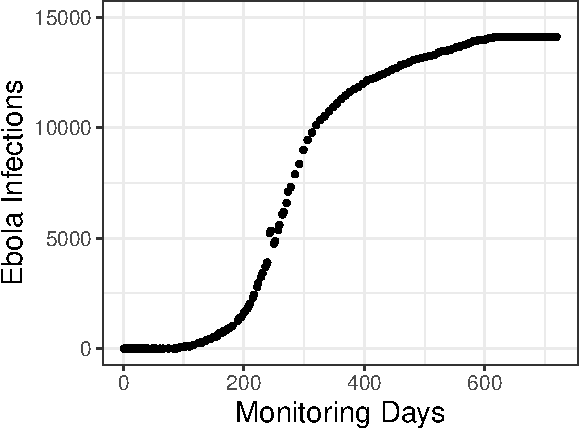
\includegraphics{series_files/figure-latex/sierra-leone-01-1.pdf}
\caption{\label{fig:sierra-leone-01}An Ebola outbreak in Sierra Leone}
\end{figure}

Constructing a model from disease dynamics is part of the field of \href{https://en.wikipedia.org/wiki/Mathematical_modelling_of_infectious_disease}{mathematical epidemiology}. How we construct a mathematical model of the spread of this outbreak largely depends on the assumptions underlying the dynamics of the disease, such as considering the rate of spread of Ebola. For our purposes here we focus on the population level (person to person) spread of Ebola. Other types of models could focus on the immune response in a single person - perhaps with a goal to design effective types of treatments to reduce the severity of infection.

Here are three initial assumptions one can make regarding the spread of Ebola:

\begin{enumerate}
\def\labelenumi{\arabic{enumi}.}
\tightlist
\item
  The infection rate is proportional to the number of people infected.
\item
  The infection rate is proportional to the number of people \textbf{not} infected.
\item
  The infection rate is proportional to the number of infected people coming into contact with those not infected.
\end{enumerate}

Let's see what each of these mathematical models would look like if we wrote down a mathematical equation. Since we are discussing \emph{rates} of infection, this means we will need a \emph{rate of change} or derivative. Let's use the letter \(I\) to represent the number of people that are infected.

\hypertarget{model-1-infection-rate-proportional-to-number-infected.}{%
\subsection{Model 1: Infection rate proportional to number infected.}\label{model-1-infection-rate-proportional-to-number-infected.}}

The first assumption states that the infection rate is proportional to the number of people infected. Translated into an equation this would be the following:

\begin{equation}
\frac{dI}{dt} = kI \label{eq:00infected}
\end{equation}

In Equation \eqref{eq:00infected} \(k\) can be thought of as a proportionality constant, with units of time\(^{-1}\) for consistency. Equation \eqref{eq:00infected} is an example of a \emph{differential equation}, which is just a mathematical equation with rates of change.

The \emph{solution} to a differential equation is a function \(I(t)\).\footnote{You may be used to working with \emph{algebraic equations} (e.g.~solve \(x^{2}-4=0\) for \(x\)). In that case the solution can be points (for our example, \(x=\pm2\)).} When we ``solve'\,' a differential equation we determine the family of functions consistent with our rate equation. There are a lot of techniques we can use to do that, and we will examine a few later.

Back to this proportionality constant \(k\) - another term for it is a \emph{parameter}. We can always try to solve an equation without specifying the parameter - and then if we wanted to plot a solution the parameter would also be specified. In some situations we may not be as concerned with the particular \emph{value} of the parameter but rather its influence on the long-term behavior of the system (this is one aspect of \href{https://en.wikipedia.org/wiki/Bifurcation_theory}{bifurcation theory}). Otherwise we can use the collected data shown above with the given model to determine the value for \(k\). This combination of a mathematical model with data is called \emph{data assimilation} or \emph{model-data fusion}.

Before we think about possible solutions let's try to reason out if the first model would be plausible. This model states that the rate of change (the amount of increase) gets larger the more people that are sick. While this may seem reasonable initially, but perhaps grows quickly unreasonable. In the case of Ebola or any other infectious disease, stringent public health measures would be enacted if the number of people infected become too large\footnote{The COVID-19 pandemic that began in 2020 is an example of the heroic efforts of public health officials.}. Following public health measures we would expect that the rate of infection would decrease and the number of deaths to slow. So perhaps the second model might be a little more plausible. At some point the number of people who are \emph{not} sick will reach zero, making the rate of infection be zero (or no increase).

\hypertarget{model-2-infection-rate-proportional-to-number-not-infected.}{%
\subsection{Model 2: Infection rate proportional to number NOT infected.}\label{model-2-infection-rate-proportional-to-number-not-infected.}}

In this description notice how we are talking about people who are sick (which we have denoted as \(I\)) and people who are \emph{not} sick. This looks like we might need to introduce another variable for the ``not sick'\,' people, which we will call \(S\), or susceptible. So the differential equation we would write down would be:

\begin{equation} 
\frac{dI}{dt} = kS  \label{eq:01notinfected}
\end{equation}

We are still using the parameter \(k\) as with the previous model. Also note we introduced the second variable \(S\) is in Equation \eqref{eq:01notinfected}. Because we have introduced another variable \(S\) we should also include a differential equation for how \(S\) changes as well. One way that we can do this is by considering our entire population as consisting of two groups of people: \(S\) and \(I\). Infection brings someone over from \(S\) to \(I\), which we have in Figure \ref{fig:initial-si}:

\begin{figure}

{\centering 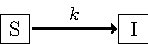
\includegraphics{series_files/figure-latex/initial-si-1} 

}

\caption{Schematic diagram for Model 1}\label{fig:initial-si}
\end{figure}

There are three reasons why I like to use diagrams like Figure \ref{fig:initial-si}: (1) they help organize my thinking about a mathematical model (2) any assumed parameters are listed, and (3) they help me to see that rates can be conserved. If I enter into the box for \(I\), then someone is leaving \(S\). So then the rate of change equation for \(S\) is \(\displaystyle \frac{dS}{dt} = -kS\). Together with the differentail equation for \(I\) I have the following:

\begin{equation}
\begin{split}
\frac{dS}{dt} &= -kS \\ 
\frac{dI}{dt} &= kS
\end{split}
\label{eq:02coupled}
\end{equation}

Equation \eqref{eq:02coupled} is an example of a \emph{coupled differential equation}. In order to ``solve'\,' the system we need to determine functions for \(S\) and \(I\). This coupled set of equations looks a little clunky, but there is something interest going on if we add the rates \(\displaystyle \frac{dS}{dt}\) and \(\displaystyle \frac{dI}{dt}\) together. Algebriacally we have:

\begin{equation} 
\frac{dS}{dt} +  \frac{dI}{dt} = \frac{d(S+I)}{dt} = 0
\end{equation}

Recall from calculus that if a rate of change equals zero then the function is constant. In this case, the variable \(S+I\) is constant, or we can also call \(S+I=N\), the number of people in the population. This means that \(S=N-I\), so we can re-write Equation \eqref{eq:02coupled} with a single equation:

\begin{equation}
\frac{dI}{dt} = k(N-I) \label{eq:02single}
\end{equation}

This second model does have some limiting behavior to this model as well. As the number of infected people reaches \(N\) (the total population size), the values of \(\displaystyle \frac{dI}{dt}\) approaches zero, meaning \(I\) doesn't change. There is one caveat to this - if there are no infected people around (\(I=0\)) \emph{the disease can still be transmitted}, which might make not good biological sense.

\hypertarget{model-3-infection-rate-proportional-to-infected-meeting-not-infected.}{%
\subsection{Model 3: Infection rate proportional to infected meeting not infected.}\label{model-3-infection-rate-proportional-to-infected-meeting-not-infected.}}

The third model rectifies some of the shortcomings of the second model (which rectified the shortcomings of the first model). This model states that the rate of infection is due to those who are sick, actually infecting those who are not sick. This would sort of scenario would also make some sense, as it focused on that \emph{transmission} of the disease are between susceptibles and infected people. So if nobody is sick (\(I=0\)) then the disease is not spread. Likewise if there are no susceptibles (\(S=0\)), the disease is not spread as well.

In this case the diagram outlining this approach looks something like this:

\begin{figure}

{\centering 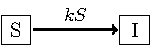
\includegraphics{series_files/figure-latex/logistic-scheme-1} 

}

\caption{Schematic diagram for Model 3}\label{fig:logistic-scheme}
\end{figure}

Notice how in Figure \ref{fig:logistic-scheme} there is an additional \(S\) associated with \(k\) to show how the rate of infection depends on \(S\). The differential equations that describe the scenario outlined in Figure \ref{fig:logistic-scheme} are the following:

\begin{align*}
\frac{dS}{dt} &= -kSI \\
\frac{dI}{dt} &= kSI
\end{align*}

Just like before for Model 2 we can combine the two equations to yield a single differential equation:

\begin{equation}
\frac{dI}{dt} = k\cdot I \cdot (N-I)
\end{equation}

Look's pretty similar to model 2, doesn't it? In this case notice the variable \(I\) outside the expression. Notice this seems to be appropriate - if \(I=0\), then there is no increase in infection. If \(I=N\) (the total population size) then there is no increase in the infection.

Let's compare these two different models graphically. For both models let's plot \(\displaystyle \frac{dI}{dt}\) versus \(I\), and just so we can plot let's \(k=1\) and \(N=10\) respectively. Plots of these functions are shown in Figure \ref{fig:threeRates-01}.

\begin{figure}
\centering
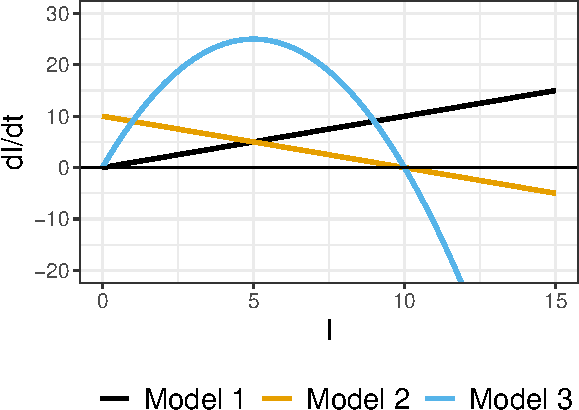
\includegraphics{series_files/figure-latex/threeRates-01-1.pdf}
\caption{\label{fig:threeRates-01}Comparing rates of change for three models}
\end{figure}

Figure \ref{fig:threeRates-01} has a lot to unpack, but we can use some of our understanding of rates of change in calculus to compare the three models. Notice how the sign of \(\displaystyle \frac{dI}{dt}\) is always positive for Model 1, indicating that the solution (\(I\)) is always increasing. For Models 2 and 3, \(\displaystyle \frac{dI}{dt}\) equals zero when \(I=10\), which also is the value for \(N\) After that case, \(\displaystyle \frac{dI}{dt}\) turns negative, meaning that \(I\) is decreasing.

In summary, examining the graphs of the rates can tell a lot about the \emph{qualitative behavior} of a solution to a differential equation even without the solution.

\hypertarget{model-solutions}{%
\section{Model solutions}\label{model-solutions}}

Let's return back to possible solutions (in this case formulas for \(I(t)\)) for our models. Usually a differential equation also has a starting or an initial value (typically at \(t=0\)) that actualizes the solution. When we state a differential equation with a starting value we have an \textbf{initial value problem}. We will represent that initial value as \(I(0)=I_{0}\), where could be considered another parameter.

With that assumption, we can (and will solve later!) the following solutions for these models:

\begin{align*}
\mbox{ Model 1 (Exponential): } & I(t) = I_{0}e^{kt} \\
\mbox{Model 2 (Saturating): } & I(t) = N-(N-I_{0})e^{-kt} \\
\mbox{Model 3 (Logistic): } & I(t) = \frac{N \cdot I_{0} }{I_{0}+(N-I_{0})e^{-kt}}
\end{align*}

Notice how I assigned the names to each model (Exponential, Saturating, and Logistic). That may not mean much at the moment, but Figure \ref{fig:three-soln} plots the three functions \(I(t)\) together when \(I_{0}=5\), \(k=0.03\), and \(N=4000\).

\begin{figure}
\centering
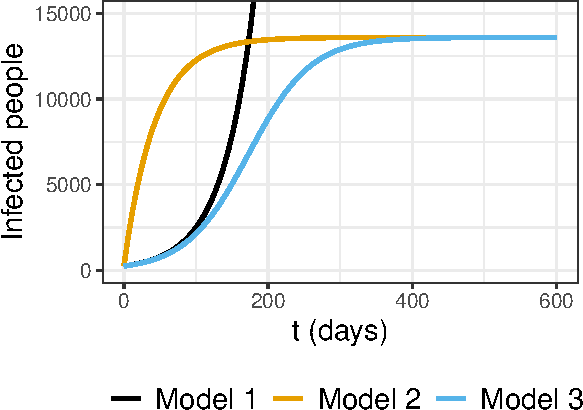
\includegraphics{series_files/figure-latex/three-soln-1.pdf}
\caption{\label{fig:three-soln}Three models compared}
\end{figure}

Notice how in Figure \ref{fig:three-soln} Model 1 increases quickly - it actually grows without bound off the chart! Model 2 and Model 3 have saturating behavior, but it looks like Model 3 might be the one that actually captures the trend of the data.

\hypertarget{which-model-is-best}{%
\section{Which model is best?}\label{which-model-is-best}}

All three of these scenarios describe different modeling scenarios. With the saturating and logistic models (Models 2 and 3) we have some limiting behavior the possibility that the the rate of infecion slows. Of the two models, which one is the \emph{best} one? Here could be some possible criteria we could evaluate:

\begin{itemize}
\tightlist
\item
  Do the model outputs match the data?
\item
  (For timeseries data) are the trends accurately represented?
\item
  Is the model easy to use?
\item
  How will model outputs compare with newly collected measurements?
  Here is a list of several things that go into a model:
\item
  The model complexity - how many equations do we have?
\item
  The number of parameters - a few or many?
\end{itemize}

We will also address that question later on in this textbook when we discuss \emph{model selection} (Chapter \ref{information-criteria}). Model selection is one key part of the modeling hypothesis - where we investigate the implications of a particular model analyzed. If we don't do this, we don't have an opportunity to test out what is plausible and what is believeable in our models.

\hypertarget{start-here}{%
\section{Start here}\label{start-here}}

In summary, it turns out that even with some initial assumptions we can very quickly build up a mathematical model to explain data. We have a lot more to uncover:

\begin{itemize}
\tightlist
\item
  How would you determine the parameters \(k\) and \(N\) with the collected data?
\item
  Are there other more complicated models?
\item
  What techniques are used to determine the formulas \(I(t)\)?
\item
  Are there other numerical techniques to approximate the solution \(I(t)\)?
\item
  What happens to our solutions when the parameters \(k\) and \(N\) change?
\item
  What happens to our solutions when the number of infected people change randomly for some reason?
\end{itemize}

We will study answers to these questions and more. Let's get started!

\newpage

\hypertarget{exercises}{%
\section{Exercises}\label{exercises}}

\begin{exercise}
\protect\hypertarget{exr:plot-soln}{}{\label{exr:plot-soln} }Solutions to an outbreak model of the flu are the following:
\begin{align*}
\mbox{Saturating model: } & I(t) = 3000-(2990)e^{-.1t} \\
\mbox{Logistic model: } &  I(t) = \frac{30000 }{10+(2990)e^{-.15t}},
\end{align*}

where \(t\) is in days. Use these two functions to answer the following questions:

\begin{enumerate}[label=\alph*.]
  \item Plot the saturating and logistic models when $0 \leq t \leq 100$.  
\item For both models, how would you describe the growth of the outbreak as $t$ increases?  How many people will be infected overall?  
  \item Finally, for both models evaluate $\lim_{t \rightarrow \infty} I(t)$. How do these results compare to values found on your graph?
  \end{enumerate}
\end{exercise}

~

\begin{figure}
\centering
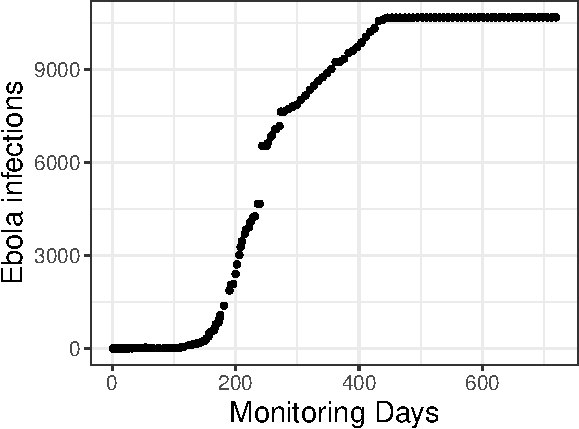
\includegraphics{series_files/figure-latex/liberia-01-1.pdf}
\caption{\label{fig:liberia-01}An Ebola outbreak in Liberia in 2014}
\end{figure}

~
\begin{exercise}
\protect\hypertarget{exr:unnamed-chunk-3}{}{\label{exr:unnamed-chunk-3} }Figure \ref{fig:liberia-01} shows the Ebola outbreak for the country of Liberia in 2014.
If we were to apply the logistic model (Model 3) based on this graphic what would be your estimate for \(N\)?
\end{exercise}
~

\begin{exercise}
\protect\hypertarget{exr:unnamed-chunk-4}{}{\label{exr:unnamed-chunk-4} }The general solution for the saturating and the logistic models are:
\begin{align*}
\mbox{Saturating model: } & I(t) = N-(N-I_{0})e^{-kt} \\
\mbox{Logistic model: } &  I(t) = \frac{N \cdot I_{0} }{I_{0}+(N-I_{0})e^{-kt}},
\end{align*}
where \(I_{0}\) is the initial number of people infected and \(N\) is the overall population size. Using the functions from Exercise \ref{exr:plot-soln} for both models, what are \(N\) and \(I_{0}\)?
\end{exercise}
~

\begin{exercise}
\protect\hypertarget{exr:unnamed-chunk-5}{}{\label{exr:unnamed-chunk-5} }The general solution for the saturating and the logistic models are:
\begin{align*}
\mbox{Saturating model: } & I(t) = N-(N-I_{0})e^{-kt} \\
\mbox{Logistic model: } &  I(t) = \frac{N \cdot I_{0} }{I_{0}+(N-I_{0})e^{-kt}},
\end{align*}
where \(I_{0}\) is the initial number of people infected and \(N\) is the overall population size. For both models carefully evaluate the limits to show \(\lim_{t \rightarrow \infty} I(t)=N\). How do your limiting values these compare to the steady-state values you found for Models 2 and 3 in Figure \ref{fig:three-soln}, where \(N=4000\)?
\end{exercise}
~

\begin{exercise}
\protect\hypertarget{exr:unnamed-chunk-6}{}{\label{exr:unnamed-chunk-6} }A model that describes the growth of sales of a product in response to advertising is the following:
\[\frac{dS}{dt} = .55\sqrt{1-S}-S, \]
where \(S\) is the product's share of the market (scaled between 0 and 1). Use this information to answer the following questions:

\begin{enumerate}[label=\alph*.]
  \item Make a plot of the function $f(S)=.55\sqrt{1-S}-S$. for $0 \leq S \leq 1$.
  \item Interpret your plot to predict when the market share will be increasing and decreasing.  At what value is $\displaystyle \frac{dS}{dt}=0$?  (This is called the \emph{steady-state} value.).
  \item  A second campaign is has the following differential equation:
  $$\frac{dS}{dt} = .2\sqrt{1-S}-S $$

What is the steady-state value and how does it compare to the previous one?
\end{enumerate}
\end{exercise}

~

\begin{exercise}
\protect\hypertarget{exr:unnamed-chunk-7}{}{\label{exr:unnamed-chunk-7} }A more general form of the advertising model is

\begin{equation}
\frac{dS}{dt} = r\sqrt{1-S}-S,
\end{equation}

where \(S\) is the product's share of the market (scaled between 0 and 1). The parameter \(r\) is related to the effectiveness of the advertising (between 0 and 1).

\begin{enumerate}[label=\alph*.]
  \item Solve $\displaystyle \frac{dS}{dt} = r\sqrt{1-S}-S$ for the steady state value (where $\displaystyle \frac{dS}{dt}=0$).  Your final answer should be expressed as a function $S(r)$.
  \item Make a plot of the steady state value as a function of $r$, where $0 \leq r \leq 1$.
  \item Based on your plot, what can you conclude about the steady state value as the effectiveness of the advertising increases?
  \end{enumerate}
\end{exercise}

~

\begin{exercise}
\protect\hypertarget{exr:unnamed-chunk-8}{}{\label{exr:unnamed-chunk-8} }A common saying is ``You are what you eat.'\,' This saying is mostly true and can be related in a mathematical model! Here's how: an equation that relates a consumer's nutrient content (denoted as \(y\)) to the nutrient content of food (denoted as \(x\)) is given by:
\begin{equation}
 y = c x^{1/\theta},
\end{equation}
where \(\theta \geq 1\) and \(c\) are both constants is a constant. Units on \(x\) and \(y\) are expressed as a proportion of a given nutrient (such as nitrogen or carbon). Let's start with an example when \(c=1\) and \(\theta = 1\). Our function then is \(y=x\). In this case the point \((0.05,0.05)\) would say that if an animal ate food that was 5\% nitrogen, their body composition would be 5\% as well.

\begin{enumerate}[label=\alph*.]
\item  Now assume that $c=1$. How does the nutrient content of the consumer compare to the food when $\theta=2$?  Draw a sample curve and interpret it, contrasting it to when $\theta = 1$.
\item Now assume that $c=1$. How does the nutrient content of the consumer compare to the food when $\theta=5$?  Draw a sample curve and interpret it, contrasting this curve to the previous two.
\item What do you think will happen when $\theta \rightarrow \infty$? Draw some sample curves to help illustrate your findings.
\end{enumerate}
\end{exercise}

~

\begin{exercise}
\protect\hypertarget{exr:unnamed-chunk-9}{}{\label{exr:unnamed-chunk-9} }A model for the outbreak of a cold virus assumes that the rate people get infected is proportional to infected people contacting susceptible people, as with Model 3 (the Logistic model). However people who are infected can also recover and become susceptible again with rate \(\alpha\). Construct a diagram similar Model 3 for this scenario and also write down what you think the system of differential equations would be.
\end{exercise}
~

\begin{exercise}
\protect\hypertarget{exr:unnamed-chunk-10}{}{\label{exr:unnamed-chunk-10} }A model for the outbreak of the flu assumes that the rate people get infected is proportional to infected people contacting susceptible people, as in Model 3. However people also account for recovering from the flu, denoted with the variable \(R\). Assume that the rate of recovery is proportional to the number of infected people with parameter \(\beta\). Construct a diagram like Model 3 for this scenario and also write down what you think the system of differential equations would be.
\end{exercise}
~
\begin{exercise}
\protect\hypertarget{exr:unnamed-chunk-11}{}{\label{exr:unnamed-chunk-11} }Organisms that live in a saline environment biochemically maintain the amount of salt in their blood stream. An equation that represents the level of \(S\) in the blood is the following:

\[\frac{dS}{dt} = I + p \cdot (W - S), \]

where the parameter \(I\) represents the active uptake of salt, \(p\) is the permeability of the skin, and \(W\) is the salinity in the water. Use this information to answer the following questions:

\begin{enumerate}[label=\alph*.]
  \item What is that value of $S$ at \emph{steady state}, or when $\displaystyle \frac{dS}{dt} = 0$?  Your final answer should be a function $S(I,p,W)$.
  \item Witn the steady state solution, Use your what parameters ($I$, $p$, or $W$) cause the steady state value $S$ to increase?
  \end{enumerate}
\end{exercise}

~

\begin{exercise}
\protect\hypertarget{exr:unnamed-chunk-12}{}{\label{exr:unnamed-chunk-12} }The immigration rate of bird species (species per time) from a mainland to an offshore island is \(I_{m} \cdot (1-S/P)\), where \(I_{m}\) is the maximum immigration rate, \(P\) is the size of the source pool of species on the mainland, and \(S\) is the number of species already occupying the island. Further, the extinction rate is \(E \cdot S / P\), where \(E\) is the maximum extinction rate. The growth rate of the number of species on the island is the immigration rate minus the extinction rate.

\begin{enumerate}[label=\alph*.]
\item Make representative plots of the of the immigration and the extinction rates as a function of $S$.  You may set $I_{m}$, $P$, and $E$ all equal to 1.
\item Determine the number of species for which the net growth rate is zero, or the number of species is in equilibrium.  Express your answer as $S$ as a function of $I_{m}$, $P$, and $E$.
\item Suppose that two islands of the same size are at different distances from the mainland. Birds arrive from the source pool and they have the same extinction rate on each island.  However the maximum immigration rate is larger for the island farther away.  Which of the two islands will have the larger number of species at equilibrium?
\end{enumerate}
\end{exercise}

~

\begin{exercise}
\protect\hypertarget{exr:unnamed-chunk-13}{}{\label{exr:unnamed-chunk-13} }This problem relates to animal size and volume. Assume that an animal assimilates nutrients at a rate \(R\) proportional to its surface area. Also assume that it uses nutrients at a rate proportional to its volume. You may assume that the size of the animal is implicitly a function of the nutrient intake and usage. Determine the size of the animal if its intake and use rates were in balance (meaning \(R\) is set to zero), assuming the animal is the following shapes:

\begin{enumerate}[label=\alph*.]
\item A sphere (assume size is measured with radius $r$) \emph{Note:} first determine the geometric formulas for surface area and volume.
\item A cube (assume size is measured with length $l$)
\end{enumerate}

\emph{Hint:} For both of these problems your goal is to determine a numeric value of \(r\) and \(l\).
\end{exercise}

\hypertarget{r-intro-02}{%
\chapter{Introduction to R}\label{r-intro-02}}

The primary tool we have to analyze models will be \texttt{R} and \texttt{RStudio}, which are commonly used for scientific and statistical computations. This is an exciting program and powerful program to learn! Admittedly learning a software requires a learning curve, however I think it is worth it. With \texttt{R} you will have enormous flexibility to efficiently utilize data, design effective visualizations, and process statistical models.

\hypertarget{r-and-rstudio}{%
\section{R and RStudio}\label{r-and-rstudio}}

We will use a lot with RStudio, which is an Integrated Development Environment for R.
These are two separate downloads and files, which can be found here:

\begin{itemize}
\tightlist
\item
  R: (\url{https://cran.r-project.org/mirrors.html}){[}Link to download mirror{]} (you need to select a location to download from; choose any one that is geographically close to you.)
\item
  RStudio: (\url{https://www.rstudio.com/products/rstudio/download/}){[}Choose RStudio desktop - the free version{]}.
\end{itemize}

\hypertarget{why-do-we-have-two-programs}{%
\subsection{Why do we have two programs?}\label{why-do-we-have-two-programs}}

Think of R as your basic program - this is the engine that does the computation. RStudio was developed as an Integrated Development Environment - meaning a place where you can see everything you are working on in one place. Figure \ref{fig:r-studio-pane} shows an example of an RStudio pane that I have:

\begin{figure}

{\centering 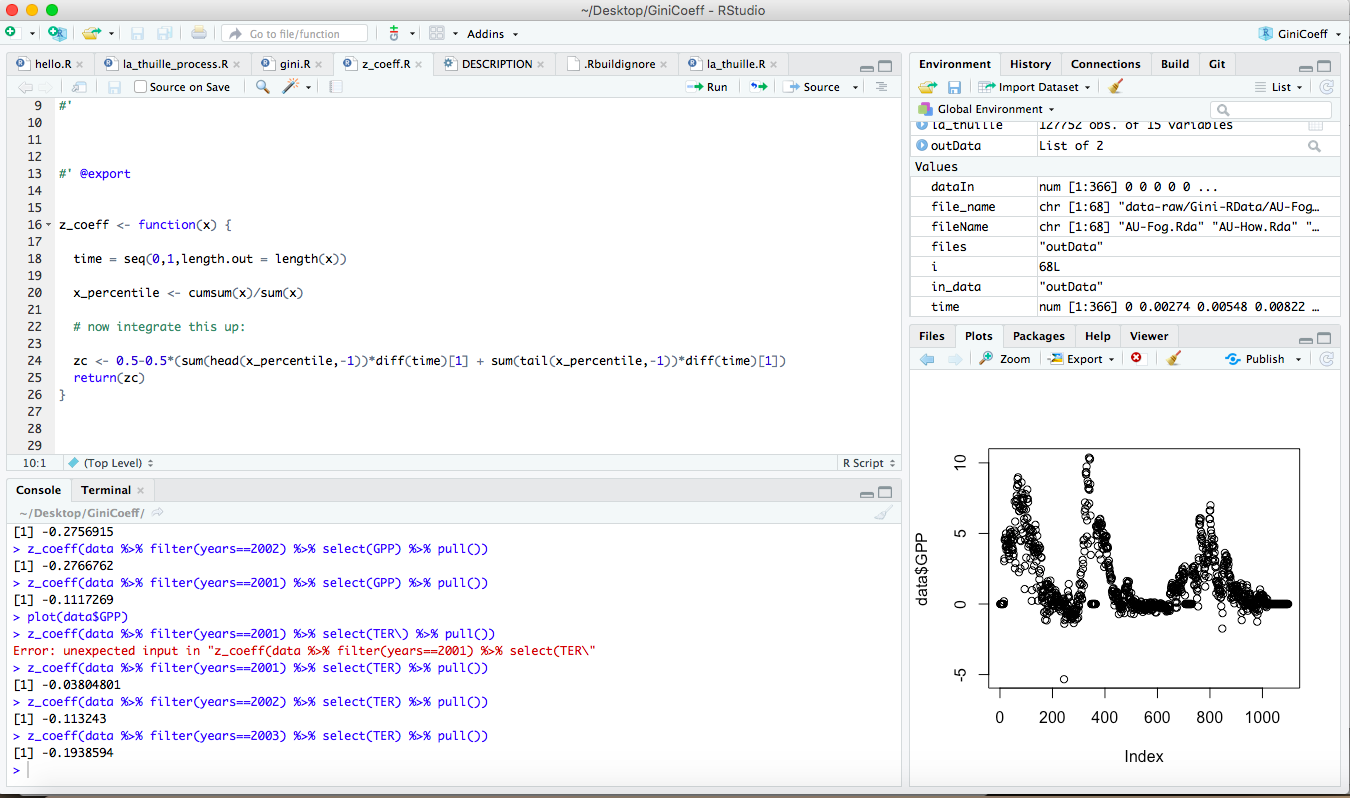
\includegraphics[width=5in]{figures/02-intro/rStudio-pane} 

}

\caption{A sample RStudio pane from one of my projects.}\label{fig:r-studio-pane}
\end{figure}

There are 4 key panels that I work with, clockwise from the top:

\begin{itemize}
\tightlist
\item
  The \textbf{source} window is in the upper left - notice how those have different tabs associated with them. You can have multiple source files that you can toggle between. For the moment think of these as commands that you will want to send to R.
\item
  The \textbf{environment} and \textbf{history} pane - these tables allow you to see what variables are stored locally in your environment, or the history of commands.
\item
  The \textbf{files} and \textbf{plots} command (a simple plot I was working on is shown currently), but you can toggle between the tabs. The files tab shows the files in the current Rstudio project directory.
\item
  Finally, the \textbf{console} pane is the place where R works and runs commands. You can type in there directly, otherwise we will also just ``send'\,' commands from the source down to the console.
\end{itemize}

Now we are ready to work with R and RStudio!

\hypertarget{first-steps-getting-acquainted-with-r}{%
\section{First steps: getting acquainted with R}\label{first-steps-getting-acquainted-with-r}}

Let's get started! Open up RStudio. Task one will be to create a project. A project is a central place to organize your materials for this course. You may do this already, but R can be picky about its working directory - and navigating to it. I found creating a project file is an easy way to avoid some of that fussiness. Let me describe steps in how to do this.

\begin{enumerate}
\def\labelenumi{\arabic{enumi}.}
\tightlist
\item
  In RStudio select ``File'' then ``New Project''
\item
  Next select the first option ``New Directory'' in the window - this will create a new folder on your computer.
\item
  At the next window choose New Directory or Existing Directory - it depends on where you want to place this project.
\item
  Name the project as you like.
\item
  Click the ``Create Project'' button.
\end{enumerate}

\hypertarget{working-with-r}{%
\subsection{``Working'' with R}\label{working-with-r}}

Our next step: where do we get R to do something? For example if we wanted to compute of \texttt{4+9} (yeah, it is 13, but this is an illustrative example), we could type this command in the R console (lower left) window. Let's try this now.

\begin{enumerate}
\def\labelenumi{\arabic{enumi}.}
\tightlist
\item
  In the console type \texttt{4+9}
\item
  Then hit enter (or return)
\item
  Is the result 13?
\end{enumerate}

Success! Now let me show you another way that works well if you have multiple lines of code to evaluate or save. Working with a script (\texttt{.R} file) is better. This will utilize the upper left hand corner of your RStudio window. (You may not have anything there when you start working on a project, so let's create one.)

\begin{enumerate}
\def\labelenumi{\arabic{enumi}.}
\tightlist
\item
  In \texttt{RStudio} select ``File'' then ``New File''
\item
  Next select the first option ``New Script''
\item
  A new window called ``UntitledX'' should appear, where X is a number. You are set to go!
\end{enumerate}

I like to use this window as a file to type stuff in and then evaluate it, which we will do next.

\textbf{Pro tip:} There are shortcuts to creating a new file: Ctrl+Shift+N (Windows and Linux) or Command+Shift+N (Mac)

\hypertarget{sending-commands-down-to-console.}{%
\subsection{Sending commands down to console.}\label{sending-commands-down-to-console.}}

Now we want to type and evaluate a command for R to do something. Click anywhere in the source file that you created and type the following:

\begin{Shaded}
\begin{Highlighting}[]
\DecValTok{4}\SpecialCharTok{+}\DecValTok{9}
\end{Highlighting}
\end{Shaded}

\begin{verbatim}
## [1] 13
\end{verbatim}

You have several options:

\begin{enumerate}
\def\labelenumi{\arabic{enumi}.}
\tightlist
\item
  Copying and pasting the command to the window. Shortcuts are Ctrl+C / Command+C for copying and Ctrl+V / Command+C for Windows / Mac.
\item
  Run the line. This means that your cursor is at the line in your source file, then clicking the `Run' button in the upper right hand side of the source window. Shortcuts are Ctrl+Enter / Command+Enter.
\end{enumerate}

\begin{figure}

{\centering 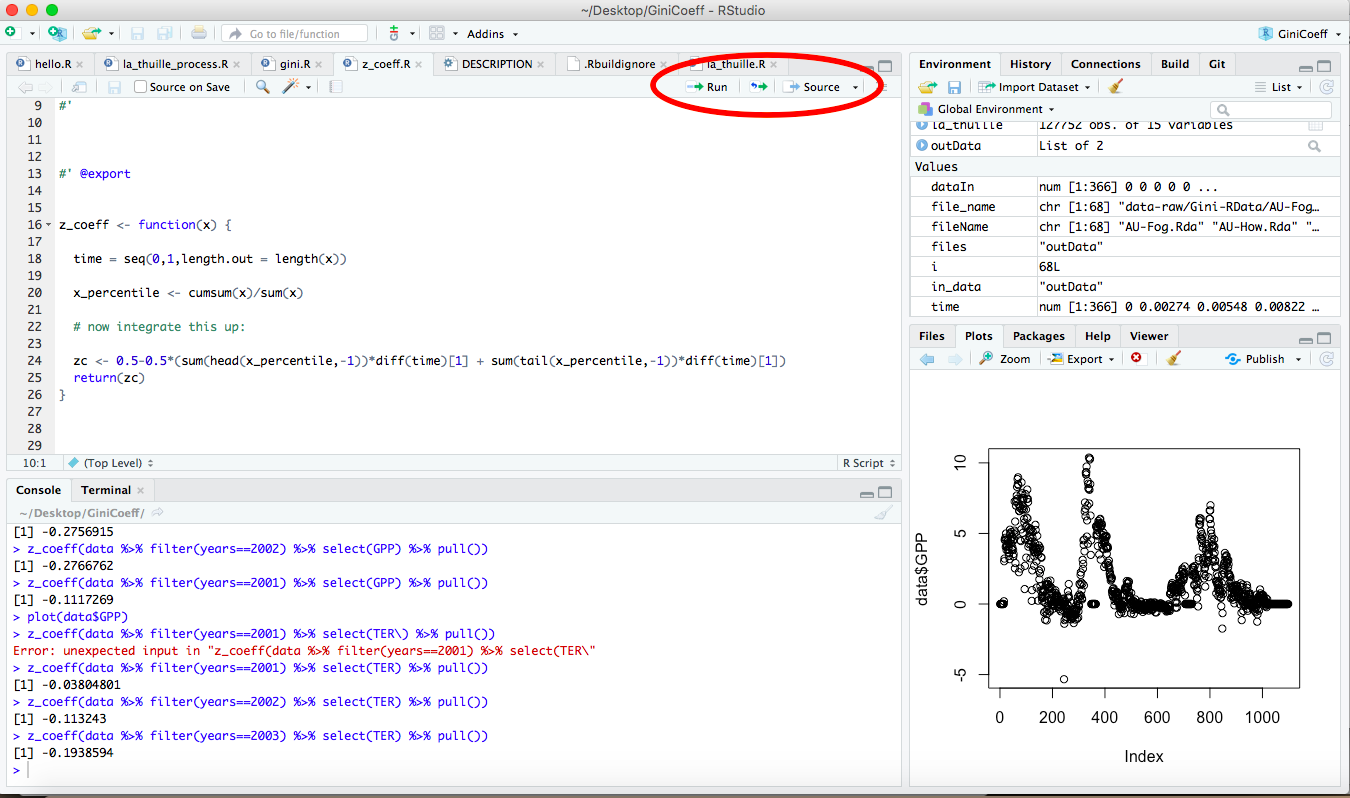
\includegraphics[width=5in]{figures/02-intro/rStudio-pane-source} 

}

\caption{Sending a command to the console.}\label{fig:unnamed-chunk-15}
\end{figure}

\begin{enumerate}
\def\labelenumi{\arabic{enumi}.}
\setcounter{enumi}{2}
\tightlist
\item
  You can also source the whole file, which means runs all the lines from top to bottom. You do this by clicking the source button, or with shortcuts Ctrl+Shift+Enter / Cmd+Shift+Enter (Windows / Mac). You can imagine this makes things easier when you have SEVERAL lines of commands to evaluate.
\end{enumerate}

Why do I like working with a script file? Well if I run some commands that have an error then it is much easier to just fix a quick mistake and then re-run the code.

It is also helpful to annotate your code with comments (\texttt{\#}), which appear as green text in RStudio.

\hypertarget{saving-your-work}{%
\subsection{Saving your work}\label{saving-your-work}}

The neat part about a source file is that it allows you to save the file (Ctrl+S / Cmd+S). The first time you do this you may need to give this a name. The location where this file will be saved is in the same directory as your \texttt{.Rproj} project file. Now you have a file that you can come back to! In general I try to use descriptive names of files to I can refer back to them later.

~

\hypertarget{increasing-functionality-with-packages}{%
\section{Increasing functionality with packages}\label{increasing-functionality-with-packages}}

One awesome versatility with R is the ability to add packages - these packages extend the functionality of R with contributed, specialized code. These are similar to apps on your phone. You can get packages from a few different places:

\begin{itemize}
\tightlist
\item
  \href{https://cran.r-project.org/}{CRAN}, which stands for Comprehensive R Archive Network. This is the clearing house for many contributed packages - and allows for easy cross platform functonality.
\end{itemize}

One key package is \href{https://www.tidyverse.org/}{\texttt{tidyverse}}, which is actually a collection of packages. If you take an introductory data science course you will most likely be learning more about this package, but to install this at the command line you type the following:

\begin{Shaded}
\begin{Highlighting}[]
\FunctionTok{install.packages}\NormalTok{(}\StringTok{\textquotesingle{}tidyverse\textquotesingle{}}\NormalTok{)}
\end{Highlighting}
\end{Shaded}

Typing this line will connect to the CRAN download mirrors and install this set of packages locally to your computer. It make take some time, but be patient.

Another package you should install is \texttt{devtools}:

\begin{Shaded}
\begin{Highlighting}[]
\FunctionTok{install.packages}\NormalTok{(}\StringTok{\textquotesingle{}devtools\textquotesingle{}}\NormalTok{)}
\end{Highlighting}
\end{Shaded}

Sometimes when you are installing packages you may be prompted to install additional packages. In this case just say yes.

\begin{itemize}
\tightlist
\item
  Github. This is another place where people can share code and packages. The code here has not been vetted through CRAN for compatibility, but if you trust the person sharing the code, it should work. In order to do this we will need to first load up the \texttt{devtools} library:
\end{itemize}

\begin{Shaded}
\begin{Highlighting}[]
\FunctionTok{library}\NormalTok{(devtools)}
\FunctionTok{install\_github}\NormalTok{(}\StringTok{"jmzobitz/demodelr"}\NormalTok{,}\AttributeTok{build\_vignettes=} \ConstantTok{TRUE}\NormalTok{)}
\end{Highlighting}
\end{Shaded}

What this command will do is pull in the package structure from my github page and install it locally.

Here is the good news: \emph{you only need to install a package once before using it!} To load the package up into your workspace you use the command \texttt{library}:

\begin{Shaded}
\begin{Highlighting}[]
\FunctionTok{library}\NormalTok{(tidyverse)}
\FunctionTok{library}\NormalTok{(demodelr)}
\end{Highlighting}
\end{Shaded}

You need to load up your these libraries \emph{each time you restart your R session}. This is part of the benefit of a script file - at the start I always declare the libraries that I will need at the start of the script file, as shown in the following figure:

\begin{figure}

{\centering 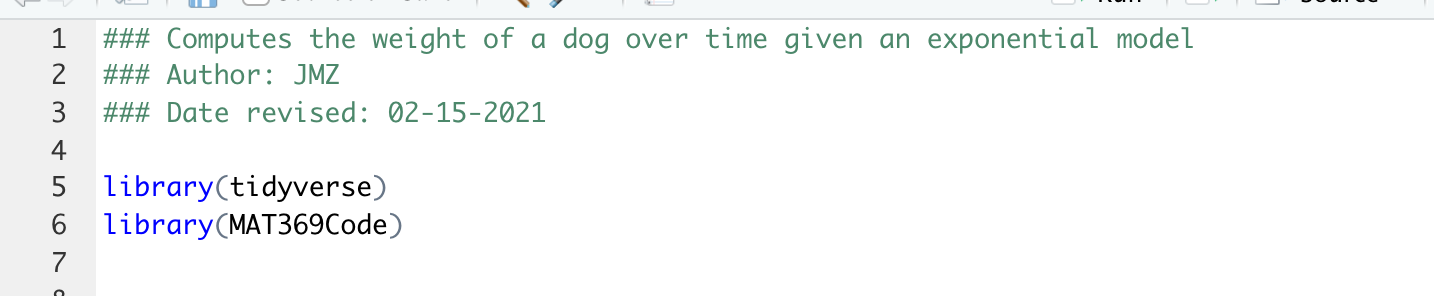
\includegraphics[width=5in]{figures/02-intro/sample-R-script} 

}

\caption{A sample R script.}\label{fig:unnamed-chunk-20}
\end{figure}

Also notice here that the first few lines of the script file I used comments \texttt{\#} to denote the basic purpose of the file, who wrote it, and the date it was last revised. This type of information is good programming practice at the start.

\hypertarget{working-with-r-variables-data-frames-and-datasets}{%
\section{Working with R: variables, data frames, and datasets}\label{working-with-r-variables-data-frames-and-datasets}}

\hypertarget{creating-variables}{%
\subsection{Creating variables}\label{creating-variables}}

The next thing we will want to do is to define variables that are stored locally. This is pretty easy to do:

\begin{Shaded}
\begin{Highlighting}[]
\NormalTok{my\_result }\OtherTok{\textless{}{-}} \DecValTok{4}\SpecialCharTok{+}\DecValTok{9}
\end{Highlighting}
\end{Shaded}

The symbol \texttt{\textless{}-} is assignment (you can use equals (=), but it is good coding practice to use the arrow for assignment). Notice how I named the variable called \texttt{my\_result}. Generally I prefer using \emph{descriptive} names for variables for the context at hand (In other words, \texttt{x} would be an odd choice - too ambiguous.) I also used snake case to string together multiple words. In practice you can use snake case, or alphabetic cases (\texttt{myResult}) or even \texttt{my.result} (although that may not be preferred practice in the long run). You can't use \texttt{my-result} because it looks like subtraction.

Here is the good news, then we can compute with the new variable, so for example \texttt{10*my\_result} should yield 130. Cool, no? As an example, let's define a sequence, spaced from 0 to 5 with spacing of 0.05. Store this in a variable called \texttt{my\_sequence}.

To do this we use the \texttt{seq} command and requires the starting value, ending value, and step size:

\begin{Shaded}
\begin{Highlighting}[]
\NormalTok{my\_sequence }\OtherTok{\textless{}{-}} \FunctionTok{seq}\NormalTok{(}\AttributeTok{from=}\DecValTok{0}\NormalTok{,}\AttributeTok{to=}\DecValTok{5}\NormalTok{,}\AttributeTok{by=}\FloatTok{0.05}\NormalTok{)}
\end{Highlighting}
\end{Shaded}

The format for the function \texttt{seq} is \texttt{seq(from=start,to=end,by=step\_size)}. The \texttt{seq} command is a pretty flexible - there are alternative ways you can generate a sequence by specifying the starting and the end values along with the number of points. If you want to know more about \texttt{seq} you can always use \texttt{?} followed by the command - that will bring up the help values:

\begin{Shaded}
\begin{Highlighting}[]
\NormalTok{?seq}
\end{Highlighting}
\end{Shaded}

Once you get more comfortable with syntax in R, you will see that \texttt{seq(0,5,0.5)} gives the same result as \texttt{seq(from=0,to=5,by=0.05)}, but it is helpful to write your code \emph{so that you can understand what it does}.

\hypertarget{data-frames}{%
\subsection{Data frames}\label{data-frames}}

A key structure in \texttt{R} is that of a data frame, which allows different types of data to be collected together. A data frame is like a spreadsheet where each column is a value and each row a value (much like you would find in a spreadsheet):

\begin{table}

\caption{\label{tab:sample-data}A data frame}
\centering
\begin{tabular}[t]{l|r|r}
\hline
  & mpg & disp\\
\hline
Mazda RX4 & 21.0 & 160\\
\hline
Mazda RX4 Wag & 21.0 & 160\\
\hline
Datsun 710 & 22.8 & 108\\
\hline
Hornet 4 Drive & 21.4 & 258\\
\hline
Hornet Sportabout & 18.7 & 360\\
\hline
\end{tabular}
\end{table}

Table \ref{tab:sample-data} shows the miles per gallon in one column (the variable \texttt{mpg} and the engine size (the variable \texttt{disp}) for different types of cars. The row names (\texttt{Mazda\ RX4}) just tell you the type of the car. Sometimes row names are not shown.

Another data frame may list solutions to a differential equation, like we did with our three infection models in Chapter \ref{intro-01}:

\begin{table}

\caption{\label{tab:model-table}Model solutions}
\centering
\begin{tabular}[t]{r|r|r|r}
\hline
time & model\_1 & model\_2 & model\_3\\
\hline
0.000000 & 5.000000 & 5.0000 & 5.000000\\
\hline
6.060606 & 5.996981 & 669.1571 & 5.995486\\
\hline
12.121212 & 7.192755 & 1222.9000 & 7.188814\\
\hline
18.181818 & 8.626962 & 1684.5848 & 8.619147\\
\hline
24.242424 & 10.347145 & 2069.5158 & 10.333332\\
\hline
\end{tabular}
\end{table}

Data frames are an example of \emph{tidy} data, where each row is an observation, each column a variable (which can be quantitative or categorical). There are several different ways to define a data frame in \texttt{R}. I am going to rely on the approach utilized by the \texttt{tidyverse}, which calls data frames \texttt{tibbles}. So for example, here is I am going to define a data frame that computes the quadratic function \(y=3x^2-2x\) for \(-5 \leq x \leq 2\).

\begin{Shaded}
\begin{Highlighting}[]
\NormalTok{x }\OtherTok{\textless{}{-}} \FunctionTok{seq}\NormalTok{(}\AttributeTok{from=}\SpecialCharTok{{-}}\DecValTok{5}\NormalTok{,}\AttributeTok{to=}\DecValTok{2}\NormalTok{,}\AttributeTok{by=}\FloatTok{0.05}\NormalTok{)}
\NormalTok{y }\OtherTok{\textless{}{-}} \DecValTok{3}\SpecialCharTok{*}\NormalTok{x}\SpecialCharTok{\^{}}\DecValTok{2}\SpecialCharTok{{-}}\NormalTok{2x}

\NormalTok{my\_data }\OtherTok{\textless{}{-}} \FunctionTok{tibble}\NormalTok{(}\AttributeTok{x=}\NormalTok{x,}
                  \AttributeTok{y=}\NormalTok{y)  }\CommentTok{\# Notice I sam specifically defining x and y}
\end{Highlighting}
\end{Shaded}

Notice that the data frame \texttt{my\_data} uses the column (variable) names of \texttt{x} and \texttt{y}. You could have also used \texttt{tibble(x,y)}, but it is helpful to name the columns in the way that you would like them to be named.

\hypertarget{reading-in-datasets}{%
\subsection{Reading in datasets}\label{reading-in-datasets}}

R has a lot of built in datasets! In fact to see all the datasets, type \texttt{data()} at the console. This will popup a new window in RStudio with the names. Cool!

If you want to see the datasets for a specific package (such as \texttt{demodelr}) you type \texttt{data(package\ =\ "demodelr")} at the console.

Perhaps what is most important is being able to read in datasets provided to you. Data come in several different types of formats, but one of the more versatile ones are csv (\textbf{c}omma \textbf{s}eparated \textbf{v}alues). What you need to do is the following:

\begin{itemize}
\tightlist
\item
  Where you have your .Rproj file located, create a folder called \texttt{data} or \texttt{datasets}
\item
  Save the file locally on your computer. Take note where you have it saved on your computer, and drag the file to your \texttt{data} folder.
\item
  To read in the file you will use the command \texttt{read\_csv}, which has the following structure:
\end{itemize}

\begin{Shaded}
\begin{Highlighting}[]
\NormalTok{in\_data }\OtherTok{\textless{}{-}} \FunctionTok{read\_csv}\NormalTok{(FILENAME)}
\end{Highlighting}
\end{Shaded}

The data gets assigned to the variable \texttt{in\_data} (You can call this variable what you want.) For example I have the following csv file of ebola data, which I read in via the following:

\begin{Shaded}
\begin{Highlighting}[]
\NormalTok{ebola }\OtherTok{\textless{}{-}} \FunctionTok{read\_csv}\NormalTok{(}\StringTok{"data/ebola.csv"}\NormalTok{)}
\end{Highlighting}
\end{Shaded}

Notice the quotes around the FILENAME. \textbf{Pro tip:} If you have the data files in the data folder, in RStudio you can type ``data'' and it may start to autocomplete - this is hand (you can also use tab.)

\hypertarget{visualization-with-r}{%
\section{Visualization with R}\label{visualization-with-r}}

Now we are ready to begin visualizing data frames. Two types of plots that we will need to make will be a scatter plot and a line plot. We are going to consider both of these separately, with examples that you should be able to customize.

\hypertarget{making-a-scatterplot}{%
\subsection{Making a scatterplot}\label{making-a-scatterplot}}

One dataset we have is the mass of a dog over time, adapted from \href{http://bscheng.com/2014/05/07/modeling-logistic-growth-data-in-r/}{here}. We have two variables here: \(D=\) the age of the dog in days and \(W=\) the weight of the dog in pounds. I have the data loaded into the \texttt{demodelr} package, which you can investigate by typing the following at the command line (I display it below as well):

\begin{Shaded}
\begin{Highlighting}[]
\FunctionTok{glimpse}\NormalTok{(wilson)}
\end{Highlighting}
\end{Shaded}

(Notice that I have assumed you have the demodelr library loaded.) You can also explore the documentation for this dataset by typing \texttt{?wilson} at the console.

\begin{table}

\caption{\label{tab:unnamed-chunk-28}Weight of a dog over time}
\centering
\begin{tabular}[t]{r|r}
\hline
days & mass\\
\hline
31 & 6.25\\
\hline
62 & 10.00\\
\hline
93 & 20.00\\
\hline
99 & 23.00\\
\hline
107 & 26.00\\
\hline
113 & 27.60\\
\hline
121 & 29.80\\
\hline
127 & 31.60\\
\hline
148 & 37.20\\
\hline
161 & 41.20\\
\hline
180 & 48.70\\
\hline
214 & 54.00\\
\hline
221 & 54.00\\
\hline
307 & 63.00\\
\hline
452 & 66.00\\
\hline
482 & 72.00\\
\hline
923 & 72.20\\
\hline
955 & 76.00\\
\hline
1308 & 75.00\\
\hline
\end{tabular}
\end{table}

Notice that this data frame has two variables: \texttt{days} and \texttt{mass}
To make a scatter plot of these data we are going to use the command \texttt{ggplot}:

\begin{Shaded}
\begin{Highlighting}[]
\FunctionTok{ggplot}\NormalTok{(}\AttributeTok{data =}\NormalTok{ wilson) }\SpecialCharTok{+} 
  \FunctionTok{geom\_point}\NormalTok{(}\FunctionTok{aes}\NormalTok{(}\AttributeTok{x =}\NormalTok{ days, }\AttributeTok{y =}\NormalTok{ mass)) }\SpecialCharTok{+}
  \FunctionTok{labs}\NormalTok{(}\AttributeTok{x=}\StringTok{\textquotesingle{}Days since birth\textquotesingle{}}\NormalTok{,}
         \AttributeTok{y=}\StringTok{\textquotesingle{}Weight (pounds)\textquotesingle{}}\NormalTok{)}
\end{Highlighting}
\end{Shaded}

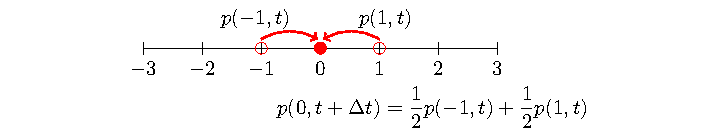
\includegraphics{series_files/figure-latex/unnamed-chunk-29-1.pdf}

Wow! This looks complicated. Let's break this down step by step:

\begin{itemize}
\tightlist
\item
  \texttt{ggplot(data\ =\ wilson)\ +} sets up the graphics structure and identifies the name of the data frame we are include.\\
\item
  \texttt{geom\_point(aes(x\ =\ days,\ y\ =\ mass))} defines the type of plot we are going to be making.\\
\item
  \texttt{geom\_point()} defines the type of plot geometry (or \emph{geom}) we are using here - in this case, a point plot.
\item
  \texttt{aes(x\ =\ days,\ y\ =\ mass)} determines the \emph{aesthetics} of the plot. On the x axis is the days variable, on the y axis is the mass variable.
\item
  The statement beginning with \texttt{labs(x=...)} defines the labels on the x and y axes.
\end{itemize}

I know this seems like a lot to write for a plot, but this structure is actually used for some more advanced data visualization. Trust me - learning how to make informative plots can be a useful skill!

\hypertarget{making-a-line-plot}{%
\subsection{Making a line plot}\label{making-a-line-plot}}

Using the same \texttt{wilson} data, later on we will discover that the function \(\displaystyle W =f(D)= \frac{70}{1+e^{2.46-0.017D}}\). represents these data. In order to make a plot of this function we can use need to first build a data frame, \texttt{plotFunction}, which has a data frame as inputs:

\begin{Shaded}
\begin{Highlighting}[]
\NormalTok{days }\OtherTok{\textless{}{-}} \FunctionTok{seq}\NormalTok{(}\DecValTok{0}\NormalTok{,}\DecValTok{1500}\NormalTok{,}\AttributeTok{by=}\DecValTok{1}\NormalTok{)  }\CommentTok{\# Choose spacing that is "smooth enough"}
\NormalTok{mass }\OtherTok{\textless{}{-}}  \DecValTok{70}\SpecialCharTok{/}\NormalTok{(}\DecValTok{1}\SpecialCharTok{+}\FunctionTok{exp}\NormalTok{(}\FloatTok{2.46{-}0.017}\SpecialCharTok{*}\NormalTok{days))}

\NormalTok{wilson\_model }\OtherTok{\textless{}{-}} \FunctionTok{tibble}\NormalTok{(}\AttributeTok{days =}\NormalTok{ days,}
                       \AttributeTok{mass =}\NormalTok{ mass)}

\FunctionTok{ggplot}\NormalTok{(}\AttributeTok{data =}\NormalTok{ wilson\_model) }\SpecialCharTok{+}
  \FunctionTok{geom\_line}\NormalTok{(}\FunctionTok{aes}\NormalTok{(}\AttributeTok{x=}\NormalTok{days,}\AttributeTok{y=}\NormalTok{mass)) }\SpecialCharTok{+} 
  \FunctionTok{labs}\NormalTok{(}\AttributeTok{x=}\StringTok{\textquotesingle{}Days since birth\textquotesingle{}}\NormalTok{,}
         \AttributeTok{y=}\StringTok{\textquotesingle{}Weight (pounds)\textquotesingle{}}\NormalTok{)}
\end{Highlighting}
\end{Shaded}

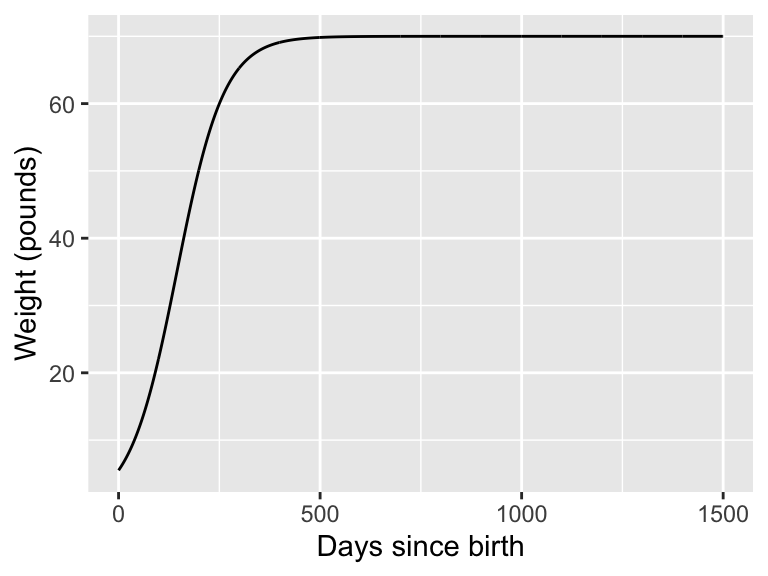
\includegraphics{series_files/figure-latex/unnamed-chunk-30-1.pdf}

Notice that once we have the data frame set up, the structure is very similar to the scatter plot - but this time we are calling using \texttt{geom\_line()} than \texttt{geom\_point}.

\hypertarget{changing-options}{%
\subsection{Changing options}\label{changing-options}}

Want a different color? Thicker line? That is fairly easy to do. For example if we wanted to make either our points or line a different color, we can just choose the following:

\begin{Shaded}
\begin{Highlighting}[]
\FunctionTok{ggplot}\NormalTok{(}\AttributeTok{data =}\NormalTok{ wilson) }\SpecialCharTok{+} 
  \FunctionTok{geom\_point}\NormalTok{(}\FunctionTok{aes}\NormalTok{(}\AttributeTok{x =}\NormalTok{ days, }\AttributeTok{y =}\NormalTok{ mass), }\AttributeTok{color=}\StringTok{\textquotesingle{}red\textquotesingle{}}\NormalTok{,}\AttributeTok{size=}\DecValTok{2}\NormalTok{) }
  \FunctionTok{labs}\NormalTok{(}\AttributeTok{x=}\StringTok{\textquotesingle{}Days since birth\textquotesingle{}}\NormalTok{,}
         \AttributeTok{y=}\StringTok{\textquotesingle{}Weight (pounds)\textquotesingle{}}\NormalTok{)}
\end{Highlighting}
\end{Shaded}

Notice how the command \texttt{color=\textquotesingle{}red\textquotesingle{}} was applied \emph{outside} of the aes - which means it gets mapped to each of the points in the data frame. \texttt{size=2} refers to the size (in millimeters) of the points. I've linked more options about the colors and sizes you can use here:

\begin{itemize}
\tightlist
\item
  \textbf{Named colors in R:} \href{https://www.r-graph-gallery.com/42-colors-names.html}{LINK} Scroll down to ``Picking one color in R'' - you can see the list of options!
\item
  \textbf{More colors:} \href{http://www.cookbook-r.com/Graphs/Colors_(ggplot2)/}{LINK}. More information about working with colors.
\item
  \textbf{Using hexadecimal colors:} \href{http://www.cookbook-r.com/Graphs/Colors_(ggplot2)/\#hexadecimal-color-code-chart}{LINK} (You specify these by the code so \texttt{"\#FF3300"} is a red color.)
\item
  \textbf{Changing sizes of lines and points:} \href{https://ggplot2.tidyverse.org/articles/ggplot2-specs.html}{LINK}
\end{itemize}

\hypertarget{combining-scatter-and-line-plots.}{%
\subsection{Combining scatter and line plots.}\label{combining-scatter-and-line-plots.}}

This is actually easy to do, especially since we are combining both the plot geoms together. Try running the following code (I am still using the data frame \texttt{wilson\_model} as defined above:

\begin{Shaded}
\begin{Highlighting}[]
\FunctionTok{ggplot}\NormalTok{(}\AttributeTok{data =}\NormalTok{ wilson) }\SpecialCharTok{+}
  \FunctionTok{geom\_point}\NormalTok{(}\FunctionTok{aes}\NormalTok{(}\AttributeTok{x =}\NormalTok{ days, }\AttributeTok{y =}\NormalTok{ mass),}\AttributeTok{color=}\StringTok{\textquotesingle{}red\textquotesingle{}}\NormalTok{) }\SpecialCharTok{+}
  \FunctionTok{geom\_line}\NormalTok{(}\AttributeTok{data =}\NormalTok{ wilson\_model, }\FunctionTok{aes}\NormalTok{(}\AttributeTok{x=}\NormalTok{days,}\AttributeTok{y=}\NormalTok{mass)) }\SpecialCharTok{+}
  \FunctionTok{labs}\NormalTok{(}\AttributeTok{x=}\StringTok{\textquotesingle{}Days since birth\textquotesingle{}}\NormalTok{,}
         \AttributeTok{y=}\StringTok{\textquotesingle{}Weight (pounds)\textquotesingle{}}\NormalTok{)}
\end{Highlighting}
\end{Shaded}

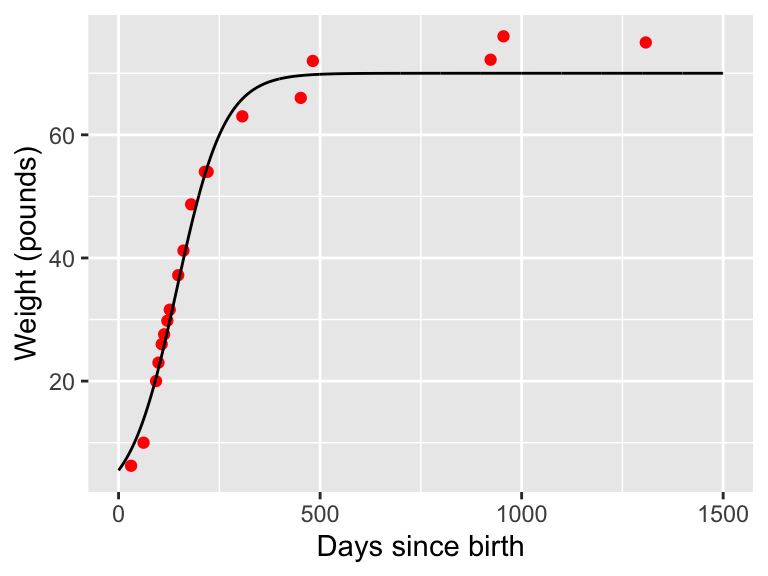
\includegraphics{series_files/figure-latex/unnamed-chunk-32-1.pdf}

Notice in the above code a subtle difference when I added in the dataset \texttt{wilson\_model} with \texttt{geom\_line}: you need to name the \texttt{data} bringing in a new data frame to a plot geom.

While it may be useful to have a legend to the plot, for this course we will make plots where this the context will be more apparent. Additional reading on legends can be found \href{http://www.cookbook-r.com/Graphs/Legends_(ggplot2)/}{here}.

\hypertarget{defining-functions}{%
\section{Defining functions}\label{defining-functions}}

We will study lots of other built-in functions for this course, but you may also be wondering how you define your own function (let's say \(y=x^{3}\)). We need the following construct:

\begin{Shaded}
\begin{Highlighting}[]
\NormalTok{function\_name }\OtherTok{\textless{}{-}} \ControlFlowTok{function}\NormalTok{(inputs) \{}
  
  \CommentTok{\# Code}
  
  \FunctionTok{return}\NormalTok{(outputs)}
\NormalTok{\}}
\end{Highlighting}
\end{Shaded}

Here \texttt{function\_name} serves as what you call the function, inputs are what you need in order to run the function, and outputs are what gets returned. So if we are doing \(y=x^{3}\) then we will call that function \texttt{cubic}:

\begin{Shaded}
\begin{Highlighting}[]
\NormalTok{cubic }\OtherTok{\textless{}{-}} \ControlFlowTok{function}\NormalTok{(x) \{}
\NormalTok{  y}\OtherTok{=}\NormalTok{x}\SpecialCharTok{\^{}}\DecValTok{3}
  \FunctionTok{return}\NormalTok{(y)}
\NormalTok{\}}
\end{Highlighting}
\end{Shaded}

So now if we want to evaluate \(y(2)=2^{3}\) we type \texttt{cubic(2)}. Neat! Now let's make a plot of the graph \(y=x^{3}\) using the function defined as \texttt{cubic}. Here is the \texttt{R} code that will accomplish this:

\begin{Shaded}
\begin{Highlighting}[]
\NormalTok{x }\OtherTok{\textless{}{-}} \FunctionTok{seq}\NormalTok{(}\AttributeTok{from =} \DecValTok{0}\NormalTok{, }\AttributeTok{to =} \DecValTok{2}\NormalTok{, }\AttributeTok{by =} \FloatTok{0.05}\NormalTok{)}
\NormalTok{y }\OtherTok{\textless{}{-}} \FunctionTok{cubic}\NormalTok{(x)}

\NormalTok{my\_data }\OtherTok{\textless{}{-}} \FunctionTok{tibble}\NormalTok{(}\AttributeTok{x=}\NormalTok{x,}\AttributeTok{y=}\NormalTok{y)}

\FunctionTok{ggplot}\NormalTok{(}\AttributeTok{data =}\NormalTok{ my\_data) }\SpecialCharTok{+}
  \FunctionTok{geom\_line}\NormalTok{(}\FunctionTok{aes}\NormalTok{(}\AttributeTok{x=}\NormalTok{x,}\AttributeTok{y=}\NormalTok{y)) }\SpecialCharTok{+}
  \FunctionTok{labs}\NormalTok{(}\AttributeTok{x=}\StringTok{\textquotesingle{}x\textquotesingle{}}\NormalTok{,}
         \AttributeTok{y=}\StringTok{\textquotesingle{}y\textquotesingle{}}\NormalTok{)}
\end{Highlighting}
\end{Shaded}

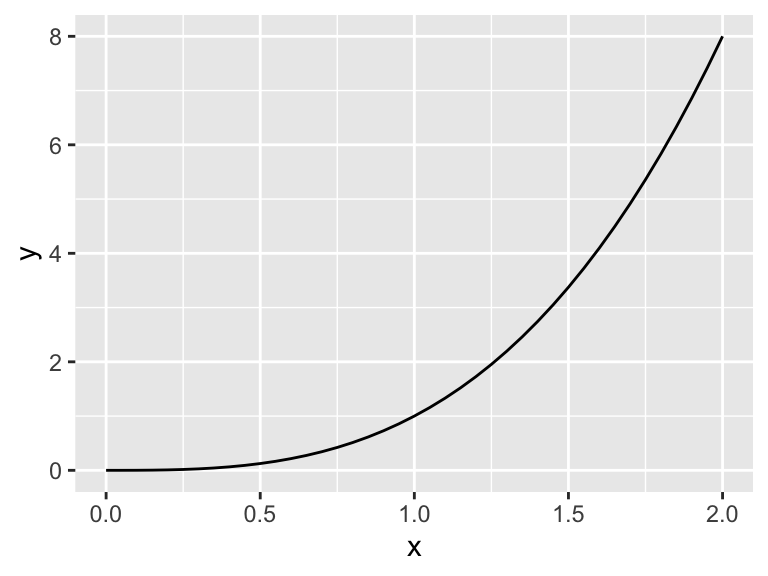
\includegraphics{series_files/figure-latex/unnamed-chunk-35-1.pdf}

\hypertarget{functions-with-inputs}{%
\subsection{Functions with inputs}\label{functions-with-inputs}}

Sometimes you may want to define a function with different input parameters, so for example the function \(y=x^{3}+c\). To define that, we can modify the function to have input variables:

\begin{Shaded}
\begin{Highlighting}[]
\NormalTok{cubic\_revised }\OtherTok{\textless{}{-}} \ControlFlowTok{function}\NormalTok{(x,c) \{}
\NormalTok{  y}\OtherTok{=}\NormalTok{x}\SpecialCharTok{\^{}}\DecValTok{3}\SpecialCharTok{+}\NormalTok{c}
  \FunctionTok{return}\NormalTok{(y)}
\NormalTok{\}}
\end{Highlighting}
\end{Shaded}

So if we want to plot what happens for different values of \texttt{c} we have the following:

\begin{Shaded}
\begin{Highlighting}[]
\NormalTok{x }\OtherTok{\textless{}{-}} \FunctionTok{seq}\NormalTok{(}\AttributeTok{from =} \DecValTok{0}\NormalTok{, }\AttributeTok{to =} \DecValTok{2}\NormalTok{, }\AttributeTok{by =} \FloatTok{0.05}\NormalTok{)}


\NormalTok{my\_data\_revised }\OtherTok{\textless{}{-}} \FunctionTok{tibble}\NormalTok{(}\AttributeTok{x=}\NormalTok{x,}
                  \AttributeTok{c\_zero=}\FunctionTok{cubic\_revised}\NormalTok{(x,}\DecValTok{0}\NormalTok{),}
                  \AttributeTok{c\_pos1=}\FunctionTok{cubic\_revised}\NormalTok{(x,}\DecValTok{1}\NormalTok{),}
                  \AttributeTok{c\_pos2=}\FunctionTok{cubic\_revised}\NormalTok{(x,}\DecValTok{2}\NormalTok{),}
                  \AttributeTok{c\_neg1=}\FunctionTok{cubic\_revised}\NormalTok{(x,}\SpecialCharTok{{-}}\DecValTok{1}\NormalTok{))}

\FunctionTok{ggplot}\NormalTok{(}\AttributeTok{data =}\NormalTok{ my\_data\_revised) }\SpecialCharTok{+}
  \FunctionTok{geom\_line}\NormalTok{(}\FunctionTok{aes}\NormalTok{(}\AttributeTok{x=}\NormalTok{x,}\AttributeTok{y=}\NormalTok{c\_zero)) }\SpecialCharTok{+}
  \FunctionTok{geom\_line}\NormalTok{(}\FunctionTok{aes}\NormalTok{(}\AttributeTok{x=}\NormalTok{x,}\AttributeTok{y=}\NormalTok{c\_pos1)) }\SpecialCharTok{+}
  \FunctionTok{geom\_line}\NormalTok{(}\FunctionTok{aes}\NormalTok{(}\AttributeTok{x=}\NormalTok{x,}\AttributeTok{y=}\NormalTok{c\_pos2)) }\SpecialCharTok{+}
  \FunctionTok{geom\_line}\NormalTok{(}\FunctionTok{aes}\NormalTok{(}\AttributeTok{x=}\NormalTok{x,}\AttributeTok{y=}\NormalTok{c\_neg1)) }\SpecialCharTok{+}
  \FunctionTok{labs}\NormalTok{(}\AttributeTok{x=}\StringTok{\textquotesingle{}x\textquotesingle{}}\NormalTok{,}
         \AttributeTok{y=}\StringTok{\textquotesingle{}y\textquotesingle{}}\NormalTok{)}
\end{Highlighting}
\end{Shaded}

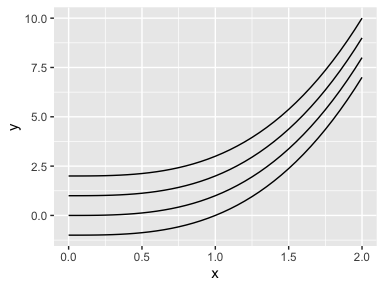
\includegraphics{series_files/figure-latex/unnamed-chunk-37-1.pdf}

Notice how I defined multiple columns of the data frame \texttt{my\_data\_revised} in the \texttt{tibble} command, and then used mutiple \texttt{geom\_line} commands to plot the data. Since we had combined the different values of \texttt{c} in a single data frame we didn't need to define the \texttt{data} with each instance of \texttt{geom\_line}.

\hypertarget{concluding-thoughts}{%
\section{Concluding thoughts}\label{concluding-thoughts}}

This is not meant to be a self-contained chapter in \texttt{R} but rather one to get you - those miles have been trod by others, and here are few of my favorites that I turn to:

\begin{itemize}
\tightlist
\item
  \href{http://www.cookbook-r.com/}{\textbf{R Graphics}}. This is a go to resource for making graphics. (I also use google a lot too.)
\item
  \href{https://bookdown.org/ndphillips/YaRrr/}{\textbf{The Pirates Guide to R}}. This book promises to build your R knowledge from the ground up.
\item
  \href{http://swcarpentry.github.io/r-novice-gapminder/}{\textbf{R for Reproducible Scientific Analysis}}. This set of guided tutorials can help you build your programming skills in R.
\item
  \href{https://r4ds.had.co.nz/}{\textbf{R for Data Science}} this is a useful book to take your R knowledge to the next level.
\end{itemize}

The best piece of advice: DON'T PANIC! Patience and persistence are your friend. Reach out for help, and recognize that like with any new endeavor, practice makes progress.
x
\newpage

\hypertarget{exercises-1}{%
\section{Exercises}\label{exercises-1}}

\begin{exercise}
\protect\hypertarget{exr:unnamed-chunk-38}{}{\label{exr:unnamed-chunk-38} }Create a folder on your computer and a project file where you will store all your R work for this textbook.
\end{exercise}
~
\begin{exercise}
\protect\hypertarget{exr:unnamed-chunk-39}{}{\label{exr:unnamed-chunk-39} }Install the packages \texttt{devtools}, \texttt{tidyverse} to your R installation. Once that is done, then install the package \texttt{demodelr} from my github page.
\end{exercise}
~
\begin{exercise}
\protect\hypertarget{exr:unnamed-chunk-40}{}{\label{exr:unnamed-chunk-40} }What are the variables listed in the dataset \texttt{phosphorous} in the \texttt{demodelr} library? (Hint: try the command \texttt{?phosphorous}.)
\end{exercise}
~
\begin{exercise}
\protect\hypertarget{exr:unnamed-chunk-41}{}{\label{exr:unnamed-chunk-41} }Make a scatterplot (\texttt{geom\_point()}) of the dataset \texttt{phosphorous} in the \texttt{demodelr} library. Be sure to label the axes.
\end{exercise}
~

\begin{exercise}
\protect\hypertarget{exr:unnamed-chunk-42}{}{\label{exr:unnamed-chunk-42} }Change the line plot of Wilson's weight over time so the line is blue and the size is 4.
\end{exercise}
~

\begin{exercise}
\protect\hypertarget{exr:unnamed-chunk-43}{}{\label{exr:unnamed-chunk-43} }Change the color of the scatterplot of Wilson's weight over time to a either a hexadecimal color or a named color of your choice.
\end{exercise}
~

\begin{exercise}
\protect\hypertarget{exr:unnamed-chunk-44}{}{\label{exr:unnamed-chunk-44} }For this exercise you will do some plotting:

\begin{enumerate}[label=\alph*.]
\item Define a sequence (call this sequence $x$) that ranges between -12 to 12 with spacing of .05.
\item Also define the variable $y$ such that $y=\sin(x)$.
\item Make a scatter plot to graph $y=\sin(x)$.  Set the points to be red.
\item Make a line plot to graph $y=\sin(x)$.  Label the x-axis with your favorite book title. Label the y-axis with your favorite food to eat.
\end{enumerate}
\end{exercise}

~

\begin{exercise}
\protect\hypertarget{exr:unnamed-chunk-45}{}{\label{exr:unnamed-chunk-45} }An equation that relates a consumer's nutrient content (denoted as \(y\)) to the nutrient content of food (denoted as \(x\)) is given by: \(\displaystyle y = c x^{1/\theta}\), where \(\theta \geq 1\) and \(c\) are both constants is a constant. Let's just assume that \(c=1\) and the \(0 \leq x \leq 1\).

Write a function called \texttt{nutrient} that will make a sequence of \texttt{y} values for an input \texttt{x} and \texttt{theta} (\(theta\)). Then use that code to make a make a line plot (\texttt{geom\_line()}) for five different values of \(\theta>1\), appropriately labeling all axes.
\end{exercise}
~

\begin{exercise}
\protect\hypertarget{exr:unnamed-chunk-46}{}{\label{exr:unnamed-chunk-46} }Researchers measured the phosphorous content of \emph{Daphnia} and its primary food source algae. This is the dataset \texttt{phosphorous} in the \texttt{demodelr} library.

Researchers believe that \emph{Daphnia} has strict homeostatic regulation of the phosphorous in algae, and as such want to determine the value of \(\theta\) in the equation \(y= \displaystyle y = c x^{1/\theta}\). They have already determined that the value of \(c=1.737\).

\begin{enumerate}[label=\alph*.]
\item If you haven't already, make a scatterplot (\texttt{geom\_point()}) of the dataset \texttt{phosphorous} in the package library. Be sure to label the axes correctly.
\item Use your function \texttt{nutrient} from the previous exercise to make an initial guess for \texttt{theta} ($\theta$) that would be consistent with the data.  You can evaluate your guess by plotting (with \texttt{geom\_line()}) against the data.
\item Use guess and check to refine the value of $\theta$ that seems to work best.
\item When you have the correct value, enter in the value of $\theta$ by clicking on [here](https://tinyurl.com/day2theta).
\end{enumerate}
\end{exercise}

~

\begin{exercise}
\protect\hypertarget{exr:unnamed-chunk-47}{}{\label{exr:unnamed-chunk-47} }For this exercise you will investigate some built-in functions. Remember you can learn more about a function by typing \texttt{?FUNCTION}, where \texttt{FUNCTION} is the name.

\begin{enumerate}[label=\alph*.]
\item Explain (using your own words) what the function \texttt{runif(1,100,1000)} does.
\item Explain (using your own words) what the function \texttt{ceiling()} does, showing an example of its use.
\end{enumerate}
\end{exercise}

~
\begin{exercise}
\protect\hypertarget{exr:unnamed-chunk-48}{}{\label{exr:unnamed-chunk-48} }For this exercise you write a sample function file.

\begin{enumerate}[label=\alph*.]
\item Create a new source file and save it as \texttt{myFunction.R}.
\item Type this code the file you created: \texttt{myInteger <- ceiling(runif(1, 100, 1000))} (This will declare a variable \texttt{myInteger} that you will work with in the following steps.)
\item Determine a function in R that will \textbf{compute a cumulative sum} from 1 to the value of \texttt{myInteger}.  Modify your file so that it also computes the cumulative sum and then source your file.
\item Copy and paste your function into your homework document for evaluation.
\end{enumerate}
\end{exercise}

~
\begin{exercise}
\protect\hypertarget{exr:unnamed-chunk-49}{}{\label{exr:unnamed-chunk-49} }The Ebola outbreak in Africa in 2014 severely affected the country of Sierra Leone. A model for the number of deaths \(D\) due to ebola is given by the following equation:
\[ D(t) = \frac{K \cdot N_{0} }{N_{0} + (K-N_{0})  \exp(-rt)}, \]
where \(K = 3980\), \(N_{0}=5\) and \(r = 0.0234\). The variable \(t\) is in days. Use \texttt{geom\_line()} to visualize this curve from \(0 \leq t \leq 700\).
\end{exercise}
~
\begin{exercise}
\protect\hypertarget{exr:unnamed-chunk-50}{}{\label{exr:unnamed-chunk-50} }Consider the following piecewise function:
\begin{equation}
y =
\begin{cases}
x^2 & \text{ for } 0 \leq x < 1,\\
2-x &\text{ for } 1 \leq x \leq  2 \\
\end{cases}
\end{equation}

\begin{enumerate}[label=\alph*.]
\item Define a function in \texttt{R} that computes $y$ for $0 \leq x \leq 2$.
\item Use \texttt{geom\_line()} to generate a graph of $y(x)$ over the interval $0 \leq x \leq 2$.
\end{enumerate}
\end{exercise}

~
\begin{exercise}
\protect\hypertarget{exr:unnamed-chunk-51}{}{\label{exr:unnamed-chunk-51} }An insect's development rate \(r\) depends on temperature \(T\) (degrees Celsius) according to the following equation:
\begin{equation}
r =
\begin{cases}
0.1 & \text{ for } 17 \leq T < 27,\\
0 &\text{ otherwise.}
\end{cases}
\end{equation}

\begin{enumerate}[label=\alph*.]
\item Define a function in \texttt{R} that computes $r$ for $0 \leq T \leq 30$.
\item Use \texttt{geom\_line()} to generate a graph of $r(T)$ over the interval $0 \leq T \leq 30$.
\end{enumerate}
\end{exercise}

\hypertarget{modeling-rates-03}{%
\chapter{Modeling with rates of change}\label{modeling-rates-03}}

So far we have looked at some examples for how we can apply rates of change to develop a mathematical model, and also learned a little bit about the ways we can apply computational software such as \texttt{R}.

In this section we are going to look some additional examples of how we can translate equations with rates of change to understand phenomena. The focus here will be on writing differential equations from a contextual description.

Oftentimes when we construct differential equations from a contextual description we bring our own understanding and knowledge to this situation. How \emph{you} may write down the differential equation may be different from someone else - \emph{do not worry!} This is the fun part of modeling: models can be considered testable hypotheses that can be refined when confronted with data.

In this section I work through a few well-known examples from mathematical biology and you will apply that knowledge to develop models from context.

\hypertarget{lynx-and-hares}{%
\section{Lynx and Hares}\label{lynx-and-hares}}

Our first example is a \emph{system of differential equations}. The context is between the snowshoe hare and the Canadian lynx. Figure \ref{fig:lynx-hare} shows a picture of them below from \href{https://www.cbc.ca/news/canada/north/canseq150-genome-sequencing-lynx-hare-1.4676308}{link}

\begin{figure}
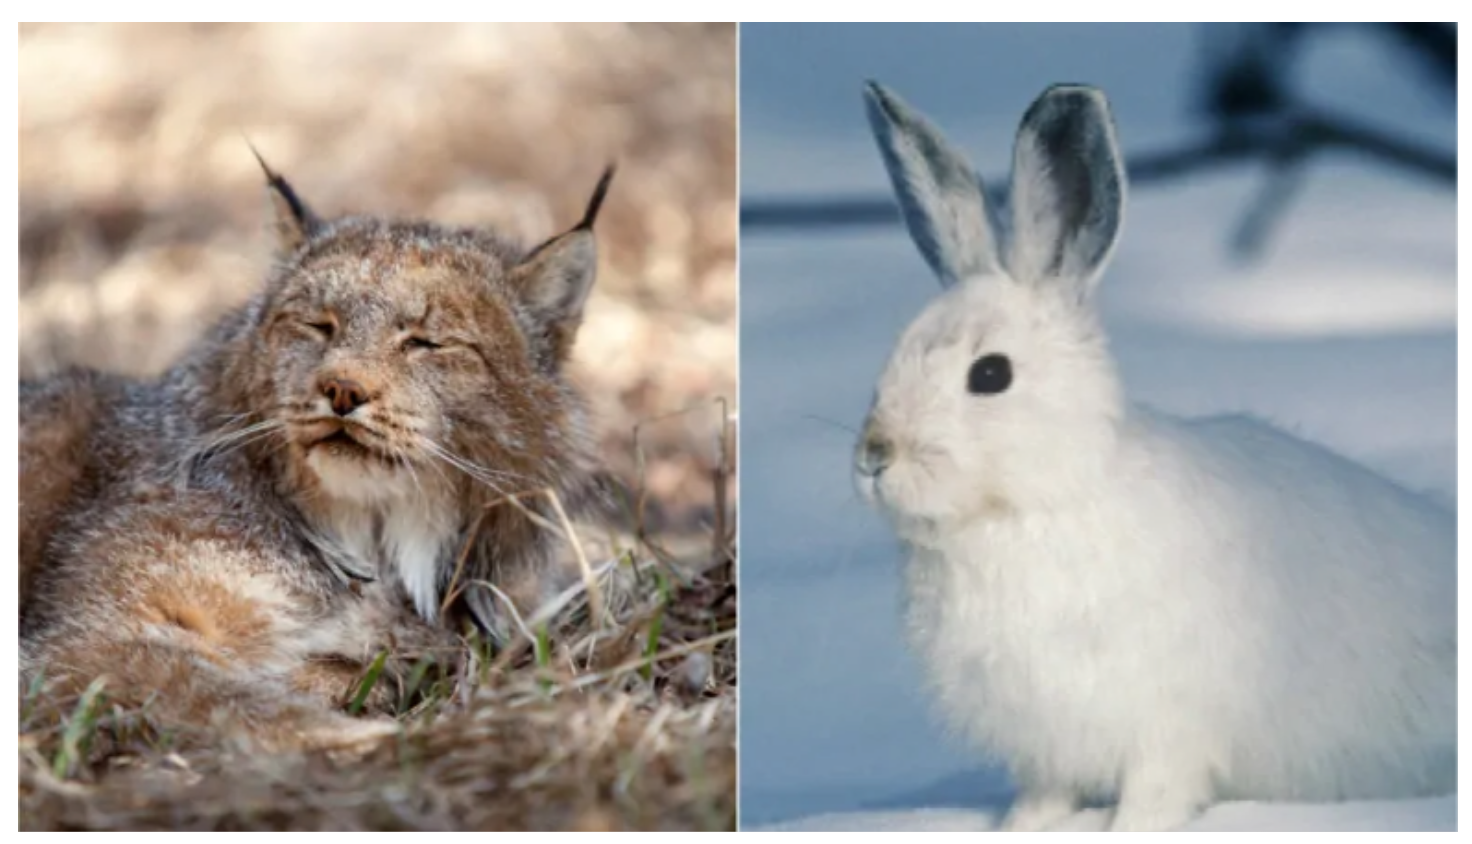
\includegraphics[width=20.44in]{figures/03-systems/lynx-hare} \caption{The lynx and hare - aren't they beautiful?}\label{fig:lynx-hare}
\end{figure}

Figure \ref{fig:lynx-hare-time} timeseries of their population is shown with this figure from (\protect\hyperlink{ref-stenseth_population_1997}{\textbf{stenseth\_population\_1997?}}).

\begin{figure}
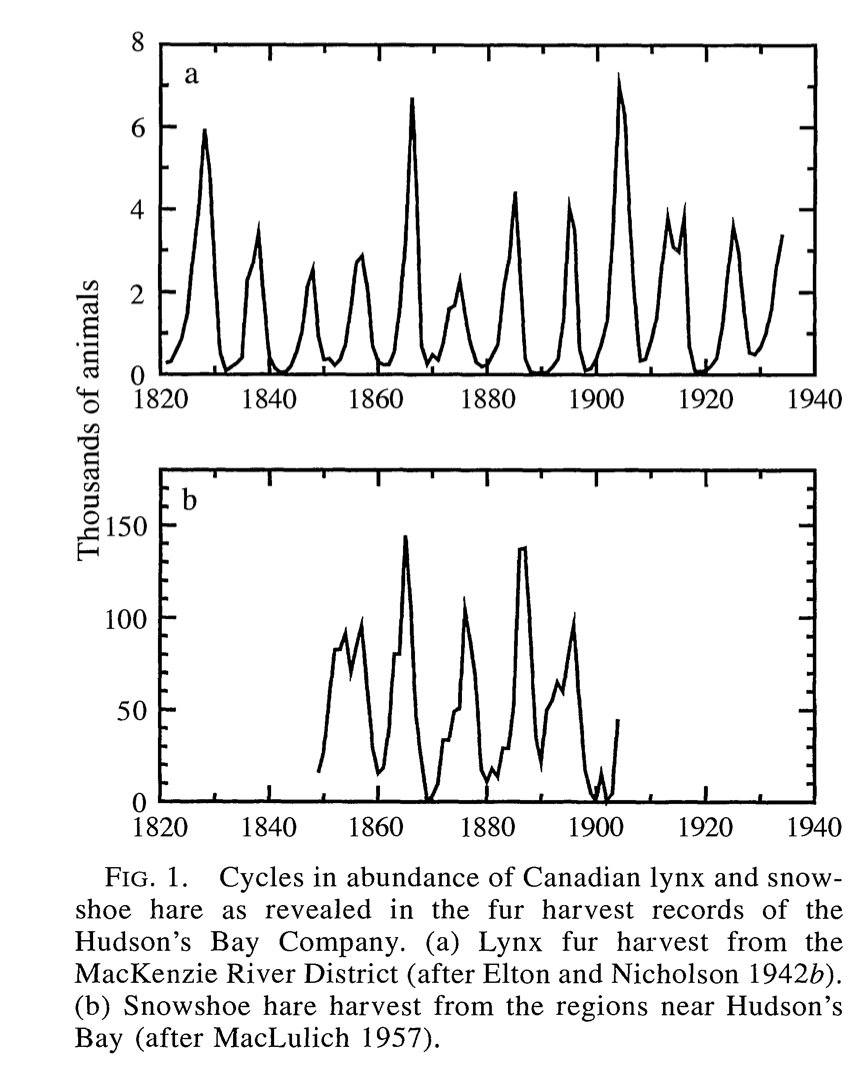
\includegraphics[width=11.89in]{figures/03-systems/lynx-hare-timeseries} \caption{A timeseries of the combined lynx and hare system.  Notice how the populations are coupled with each other.}\label{fig:lynx-hare-time}
\end{figure}

Notice how in Figure \ref{fig:lynx-hare-time} both populations seem to fluctuate periodically. One plausible reason is that the lynx prey on the snowshoe hares, which causes the population to initially decline. Once the snowshoe hare population declines, then there is less food for the lynx to survive, so their population declines. The decline in the lynx population causes the hare population to increase, and so on it goes \ldots{}

In summary it is safe to say that the two populations are \emph{coupled} to one another. But in order to understand how they are coupled together, first let's consider the two populations \emph{separately}.

The hares grow much more quickly than then lynx - in fact some hares have been known to reproduce several times a year. A reasonable assumption for large hare populations is that rate of change of the hares is proportional to the hare population. Based on this assumption Equation \eqref{eq:hareOnly} describes the rate of change of the hare population, with \(H\) is the population of the hares:

\begin{equation}
\frac{dH}{dt} = r H \label{eq:hareOnly}
\end{equation}

In this case we know that the growth rate \(r\) is positive, so then the rate of change (\(H'\)) will be positive as well, and \(H\) will be increasing. Typical values given for \(r\) in (\protect\hyperlink{ref-stenseth_population_1997}{\textbf{stenseth\_population\_1997?}}) are between 1.8 - 2.0 year\(^{-1}\). You may be thinking that the units on \(r\) seem odd - (year\(^{-1}\)). Another way to think about \(r\) is to take its inverse: \(r^{-1} \approx\) 0.5 - 0.55 years. Then \(r^{-1}\) represents the amount of time that passes before the hare population increases (pretty short!)

Let's consider the lynx now. A approach is to assume their population declines exponentially, or changes at the rate proportional to the current population. Let's consider \(L\) to be the lynx population, with the following differential equation (Equation \eqref{eq:lynxOnly}):

\begin{equation}
\frac{dL}{dt} = -dL \label{eq:lynxOnly}
\end{equation}

We assume the death rate \(d\) in Equation \eqref{eq:lynxOnly} is positive, leading to a negative rate of change for the Lynx population (and a decreasing value for \(L\)). Typical values of \(d\) are 0.9 - 2.4 year\(^{-1}\). Similar to \(r\), another way \(d\) is - like \(b\) - to take its inverse (about 0.4 - 1.1 years), which represents the amount of time that passes before the lynx population decreases by one.

The next part to consider is how they interact. Since the hares are prey for the lynx, when the lynx hunt, the hare population. We can represent this with the following adjustment to our hare equation:

\begin{equation}
\frac{dH}{dt} = r H - b HL
\end{equation}

So the parameter \(b\) represents the hunting rate. Notice how we have the term \(HL\) for this interaction. This term injects a sense of realism: if the lynx are not present (\(L=0\)), then the hare population can't decrease due to hunting. We say that the \emph{interaction} between the hares and the lynx with multiplication. Typical values for \(b\) are 480 - 870 hares \(\cdot\) lynx\(^{-1}\) year\(^{-1}\). It is okay if that unit seems a little odd to you - it should be! Here is one way to think about it. The quantity \(\displaystyle \frac{dH}{dt}\) represents the \emph{rate of change} of the hares, so it should have units of hares per year. Since the term \(bHL\) has both lynx and hare, the units for \(b\) need to account for this.

How does hunting affect the lynx population? One possibility is that it increases the lynx population:

\begin{equation}
\frac{dL}{dt} =bHL -dL
\end{equation}

Notice the symmetry between the rate of change for the hares and the lynx equations. In many cases this makes sense - if you subtract a rate from one population, then that rate should be added to the receiving population. You could also argue that there is some efficiency loss in converting the hares to lynx - not all of the hare is converted int the lynx biomass. In this situation we sometimes like to adjust the lynx equation with another parameter \(e\), representing the efficiency that hares are converted into lynx:

\begin{equation}
\frac{dL}{dt} =e\cdot bHL -dL
\end{equation}

(sometimes people just make a new parameter \(c=e \cdot b\), but for now we will just leave it as is). Equation \eqref{eq:lynx-hare-combined} shows the coupled system of differential equations:

\begin{equation}
\begin{split}
\frac{dH}{dt} &= r H - b HL \\
\frac{dL}{dt} &=ebHL -dL
\end{split}
\label{eq:lynx-hare-combined}
\end{equation}

The schematic diagram representing these interactions is the following is shown in Figure \ref{fig:lynxhare-schematic}:

\begin{figure}

{\centering 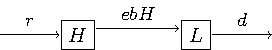
\includegraphics{series_files/figure-latex/lynxhare-schematic-1} 

}

\caption{Schematic diagram Lynx-Hare system.}\label{fig:lynxhare-schematic}
\end{figure}

Equation \eqref{eq:lynx-hare-combined} is a classical model in mathematical biology and differential equations - it is called the \emph{predator prey} model, also known as the \href{https://en.wikipedia.org/wiki/Lotka\%E2\%80\%93Volterra_equations}{Lotka-Volterra equations}. There is a lot of interesting mathematics from this system of equations that we will study later in this textbook. In later sections we will graphically and numerically analyze these equations and their solutions.

\hypertarget{the-law-of-mass-action}{%
\section{The Law of Mass Action}\label{the-law-of-mass-action}}

Notice in the previous section that the interaction between the lynx and the hare was of the form \emph{bHL} - meaning you needed both positive values of \emph{H} and \emph{L} for the interaction to continue. This law states that the rate of a change is directly proportional to the \emph{product} of the populations.

This assumption of the law of mass action is also commonly used in chemical reactions - especially in modeling enzyme dynamics. For example let's say you have a substrate \emph{A} that reactions with enzyme \emph{B} to form a product \emph{S}. Perhaps you might have seen this represented as a reaction equation:

\begin{equation}
A+B \rightarrow S
\end{equation}

How we would write the product of formation, or \(\displaystyle \frac{dS}{dt}\) is the following:

\begin{equation}
\frac{dS}{dt}= kAB,
\end{equation}

where \(k\) is the proportionality constant or the rate constant associated with the reaction. If we wanted to represent this as a schematic we would have the following diagram (Figure \ref{fig:mass-action}):

\begin{figure}

{\centering 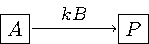
\includegraphics{series_files/figure-latex/mass-action-1} 

}

\caption{Schematic diagram of the law of mass action.}\label{fig:mass-action}
\end{figure}

We could also consider if there was a constant decay of the substrate, which we might revise Figure \ref{fig:mass-action} to Figure \ref{fig:mass-action-revised}:

\begin{figure}

{\centering 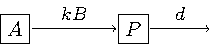
\includegraphics{series_files/figure-latex/mass-action-revised-1} 

}

\caption{Revised schematic diagram of the law of mass action with decay.}\label{fig:mass-action-revised}
\end{figure}

For this case, the rate of change of \(S\) would then be:

\begin{equation}
\frac{dS}{dt}= kAB - dS, \label{eq:mass-action-decay}
\end{equation}

You may be wondering about rates for \(A\) and \(B\). When \(S\) is formed \(A\) and \(B\) are catalyzed, so the rate of formation for \(S\) (the positive term in Equation \eqref{eq:mass-action-decay}) will be a loss for \(A\) and \(B\) (Equation \eqref{eq:mass-action-ab}):

\begin{equation}
\begin{split}
\frac{dA}{dt} &= -kAB \\
\frac{dB}{dt} &= -kAB
\end{split}
\label{eq:mass-action-ab}
\end{equation}

Both equations are similar in this case, not pending any additional inputs or outputs.

\hypertarget{establishing-species}{%
\section{Establishing species}\label{establishing-species}}

Let's look at another example where from we will determine a differential equation model from a context:

\begin{quote}
An newly introduced plant species is introduced to a region. It competes with another established species for nutrients (and is a better competitor). However, the growth rate of the new species is proportional to the difference between the current number of established species and the number of new species. You may assume that the number of established species is a constant \emph{E}.
\end{quote}

For this problem we will start by naming our variables. Let \(N\) represent number of new species and \(E\) the number of established species. We will break this down accordingly:

\begin{itemize}
\tightlist
\item
  \emph{``the growth rate of the new species''} means \(\displaystyle \frac{dN}{dt}\).
\item
  \emph{``is proportional to the difference between the current number of established species and the number of new species''} means \(\displaystyle k \cdot (E-N)\), where \(k\) is the proportionality constant. Including this parameter helps to avoid assuming we have a 1:1 correspondence between the growth rate of the new species and the population difference.
\item
  \emph{``and is a better competitor''} helps to explain why the term is \(\displaystyle k \cdot (E-N)\) insteady of \(\displaystyle k \cdot (N-E)\). We know that the newly established species will start out in much smaller numbers than \(N\). But since it is a better competitor, we would expect its rate to increase initially. So \(\displaystyle \frac{dN}{dt}\) should be \emph{positive} rather than negative. Assuming \(N < E\), then \(E-N > 0\), which guarantees that the new species will grow.
\end{itemize}

So this description could be modeled with Equation in summary we have the following model:
\begin{equation}
\frac{dN}{dt} = k(E-N)
\end{equation}

Does this equation seem familiar to you? It is similar to the second model in Chapter 1 for the spread of Ebola! While this may seem surprising, it is often the case that similar equations appear in different contexts. It is far more advantageous to learn how to analyze models qualitatively rather than memorize several different types of models and not see the connections between them.

An interesting solution to a differential equation is the \emph{steady state} or \emph{equilibrium} solution. We find this where the rate equals zero. Let's take a look how to do that for our establishing plant model

\begin{example}
\protect\hypertarget{exm:unnamed-chunk-52}{}{\label{exm:unnamed-chunk-52} }What is the steady state value for the differential equation \(\displaystyle \frac{dE}{dt} = k(E-N)\)? (That is solve for \(E\) when \(\displaystyle \frac{dE}{dt} = 0\).)
\end{example}

\begin{solution}
\iffalse{} {Solution. } \fi{}Let's solve \(\displaystyle \frac{dE}{dt} = k(E-N) = 0\). For this equation we want to express the right hand side in terms of \(E\). The parameter \(k\) is a constant \(k > 0\), so really the steady state occurs when \(E-N = 0\), or when \(N = E\).
\end{solution}

What this model tells us that eventually the new species will overtake the established species \(E\).

\hypertarget{other-types-of-functional-responses}{%
\section{Other types of functional responses}\label{other-types-of-functional-responses}}

In several examples we have seen a rate of change proportional to the current population, as in the rate of growth of the hare population is \(rH\). This is one example of what we would call a \href{https://en.wikipedia.org/wiki/Functional_response}{\emph{functional response}}. Another type of functional response assumes that the rate reaches a limiting value proportional to the population size, so \(\displaystyle \frac{dH}{dt} = \frac{rH}{1+arH}\). This is an example of a \textbf{type II functional response}. Finally the type II response has also been generalized (a \textbf{type III functional response}) \(\displaystyle \frac{dH}{dt} = \frac{rH^{2}}{1+arH^{2}}\). Figure \ref{fig:function-response} shows all three functional responses together:

\begin{figure}
\centering
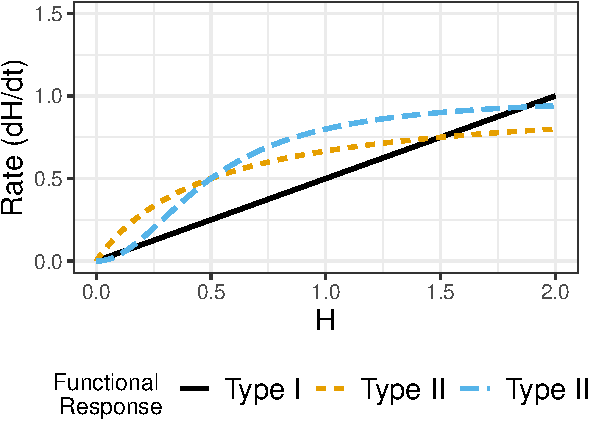
\includegraphics{series_files/figure-latex/function-response-1.pdf}
\caption{\label{fig:function-response}Comparison between Type I - Type III functional responses.}
\end{figure}

Notice the limiting behavior in the Type II and Type III functional responses. These responses are commonly used in ecology and predator-prey dynamics and in problems of how animals search for food.

\newpage

\hypertarget{exercises-2}{%
\section{Exercises}\label{exercises-2}}

\begin{exercise}
\protect\hypertarget{exr:unnamed-chunk-54}{}{\label{exr:unnamed-chunk-54} }Consider the following type of functional responses:
\begin{align}
\mbox{ Type I: } \frac{dP}{dt} &= 0.1 P \\
\mbox{ Type II: } \frac{dP}{dt} &= \frac{0.1P}{1+.03P} \\
\mbox{ Type III: } \frac{dP}{dt} &= \frac{0.1P^{2}}{1+.05P^{2}}
\end{align}

For each of the functional responses evaluate \(\displaystyle \lim_{P \rightarrow \infty} \frac{dP}{dt}\). Since these functional responses represent a rate of change of a population, what are some examples (hypothetical or actual) would each of these responses be appropriate?
\end{exercise}

~
\begin{exercise}
\protect\hypertarget{exr:unnamed-chunk-55}{}{\label{exr:unnamed-chunk-55} }A population grows according to the equation \(\displaystyle \frac{dP}{dt} = \frac{0.1P}{1+.05P} -P\).

\begin{enumerate}[label=\alph*.]
\item On the same axis, plot the equations $\displaystyle f(P) = \frac{0.1P}{1+.05P}$ and $g(P)=P$.  What are the two positive values of $P$ where $f(P)$ and $g(P)$ intersect?
\item Next algebraically determine the two steady state values of $P$, that is solve $\displaystyle \frac{dP}{dt}=0$ for $P$.  (\emph{Hint:} factor a $P$ out of the expression $\displaystyle \frac{0.1P}{1+5P} -P$.)
\item Does your algebraic solution match your graphical solutions?
\end{enumerate}
\end{exercise}

~

\begin{exercise}
\protect\hypertarget{exr:unnamed-chunk-56}{}{\label{exr:unnamed-chunk-56} }A population grows according to the equation \(\displaystyle \frac{dP}{dt} = 2P - \frac{4P^{2}}{1+P^{2}}\).

\begin{enumerate}[label=\alph*.]
\item On the same axis, plot the equations $\displaystyle f(P) = 2P$ and $\displaystyle g(P)=\frac{4P^{2}}{1+P^{2}}$.  What are the two positive values of $P$ where $f(P)$ and $g(P)$ intersect?
\item Next algebraically determine the two steady state values of $P$, that is solve $\displaystyle \frac{dP}{dt}=0$ for $P$.  (\emph{Hint:} factor a $P$ out of the expression $\displaystyle 2P - \frac{4P^{2}}{1+P^{2}}$.)
\item Does your algebraic solution match your graphical solutions?
\end{enumerate}
\end{exercise}

~

\begin{exercise}
\protect\hypertarget{exr:unnamed-chunk-57}{}{\label{exr:unnamed-chunk-57} }A population grows according to the equation \(\displaystyle \frac{dP}{dt} = \frac{aP}{1+abP} - dP\), where \(a\), \(b\) and \(d\) are parameters. Determine the two steady state values of \(P\), that is solve \(\displaystyle \frac{dP}{dt}=0\) for \(P\).
\end{exercise}
~
\begin{exercise}
\protect\hypertarget{exr:unnamed-chunk-58}{}{\label{exr:unnamed-chunk-58} }For a chemical reaction takes two chemicals \(X\) and \(Y\) to form a substrate \(Z\) through the law of mass action. However the substrate can also disassociate. The reaction schematic is the following:

\begin{equation}
X + Y \rightleftharpoons Z,
\end{equation}

where the proportionality constant \(k_+\) is associated with the formation of the substrate \(Z\) and \(k_-\) the disassociation (\(Z\) decays back to \(X\) and \(Y\)).

~

Write down a differential equation that represents the rate of reaction \(\displaystyle \frac{dZ}{dt}\).
\end{exercise}

~

\begin{exercise}
\protect\hypertarget{exr:unnamed-chunk-59}{}{\label{exr:unnamed-chunk-59} }For each of the following exercises consider the following contextual situations modeling rates of change. Name variables for each situation and write down a differential equation describing the context. Be sure to identify and briefly describe any parameters you need for your model. For each problem you will need to:

\begin{itemize}
\item Name and describe all variables.
\item Write down a differential equation.
\item Identify and describe any parameters needed.
\item Write a brief one-two sentence explanation of why your differential equation models the situation at hand.
\item Hand sketch a rough graph of what you think the solution as a function of time - \emph{note:} your solution needs to be consistent with your explanation and vice versa.
\end{itemize}

\begin{enumerate}[label=\alph*.]
\item The rate of change of an animal's body temperature is proportional to the difference in temperature between the environment.
\item A plant grows propritional to its current length $L$.  Assume this proportionality constant is $\mu$, whose rate also decreases proportional to its current value.  You will need to write down a system of two equation with variables $L$ and $\mu$.
\item A patient undergoing chemotherapy receives an injection at rate $I$. This injection decreases the rate that a tumor accumulates mass. Independent of the injection, the tumor accumulates mass at a rate proportional to the mass of the tumor.
\item A cell with radius $r$ assimilates nutrients at a rate proportional to its surface area, but uses nutrients proportional to its volume. Determine an equation that represents the rate of change of the radius. 
\item A patient undergoing chemotherapy receives an injection at rate $I$. This injection decreases the rate that a tumor accumulates mass. Independent of the injection, the tumor accumulates mass at a rate proportional to the mass of the tumor.
\item The rate that a cancer cell divides (increases in amount) is proportional to the amount of healthy cells in its surrounding environment.  You may assume that a healthy cell has a mortality $\delta_{H}$ and a cancer cell has mortality $\delta_{C}$.  Be sure to write down a system of differential equations for the population of cancer cells $C$ and healthy cells $H$.
The rate that a virus is spread to the population is proportional to the probability that a person is sick (out of $N$ total sick and healthy individuals). 
\item
\end{enumerate}
\end{exercise}

~

\begin{figure}
\centering
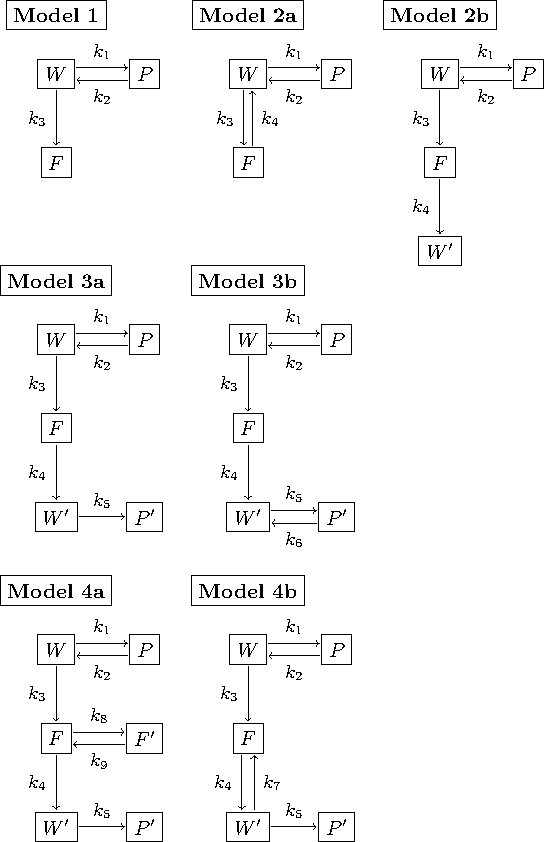
\includegraphics{series_files/figure-latex/pesticide-ch3-1.pdf}
\caption{\label{fig:pesticide-ch3}Reaction schemes.}
\end{figure}

\begin{exercise}
\protect\hypertarget{exr:unnamed-chunk-60}{}{\label{exr:unnamed-chunk-60} }You are tasked with the job of investigating the effect of a pesticide on water quality, in terms of its effects on the health of the plants and fish in the ecosystem. Different models can be created that investigate the effect of the pesticide. Different types of reaction schemes for this system are shown in Figure \ref{fig:pesticide-ch3}, where \(F\) represents the amount of pesticide in the fish, \(W\) the amount of pesticide in the water, and \(S\) the amount of pesticide in the soil. The prime (e.g.~\(F'\), \(W'\), and \(S'\) represent other bound forms of the respective state). In all seven different models can be derived. For each of the model schematics, apply the Law of Mass Action to write down a system of differential equations.
\end{exercise}

\hypertarget{euler-04}{%
\chapter{Euler's method}\label{euler-04}}

The focus of this section is on \emph{approximation} of solutions to a differential equation via a numerical method. Typically a first numerical methods one might learn to tackle this problem is \emph{Euler's method}, which is so fundamental it was popularized in the movie \href{https://www.youtube.com/watch?v=v-pbGAts_Fg}{Hidden Figures.}

The way we are going to do this is through expansion of the idea of a \emph{locally linear approximation} to the tangent line. Let's start with an example.

\begin{example}[The flu bug]
\protect\hypertarget{exm:flu-linear}{}{\label{exm:flu-linear} \iffalse (The flu bug) \fi{} }The rate of change of the flu through a population is given by the number of people infected \(t\) days after infection is, \[\displaystyle \frac{dI}{dt} = 3e^{-.025t}. \] Assuming that \(I(0)=10\), what is a locally linear approximation to this infection? Second, using your linear approximation, what would you predict is the value after one day (\(I(1)\))?
\end{example}

~

\begin{remark}
\iffalse{} {Remark. } \fi{}In order to solve this problem, we know that the locally linear approximation is to \(I(t)\) at \(t=0\) is \(L(t) = I(0) + I'(0) \cdot (t-0)\). Here, \(I(0)=10\) and \(I'(0)=3\), so \[L(t) = 10 +3t\]. Using \(L(t) \approx I(t)\), we have \(L(1)=10 + 3 = 13\). So our model predicts there will be 13 people sick.
\end{remark}

~

Notice in Example \ref{exm:flu-linear} we used two pieces of information: the (given) value of the function at \(t=0\) and the estimate of the derivative from the rate of change.

It may be helpful to compare our prediction from \(L(1)\) to the actual value. The solution to the differential equation in Example \ref{exm:flu-linear} is \(I(t) = 130-120e^{-.025t}\) (you should verify this is the case by differentation). Let's compare in the following table:

\begin{longtable}[]{@{}lll@{}}
\toprule
\(t\) & Linear approximation & Actual Solution \\
\midrule
\endhead
0 & 10 & 10 \\
1 & 13 & 12.96 \\
\bottomrule
\end{longtable}

Not too bad, huh? Our approximation at \(L(1)\) is an \emph{overestimate}, mainly because the actual solution is concave down, but it isn't that far off.

Let's build this solution out a little more by computing the rate of change at \(t=1\), assuming that thirteen people is a pretty close estimate of the \(I\) at \(t=1\). What we could do is to build \emph{another} linear approximation using the differential equation. So the locally linear approximation is to \(I(t)\) at \(t=1\) is

\[ L(t) = I(1) + I'(1) \cdot (t-1) \].

Here, \(I(1)=13\) and \(I'(1)=2.92\), and \(L(t) = 13 +2.92(t-1).\)

Assuming that \(L(t) \approx I(t)\), we can evaluate \(L(t)\) at \(t=2\) \emph{as an approximation} for \(I(2)\): have \(L(2)=13 + 2.92 = 15.92\). Comparing this to the actual solution at \(t=2\), we have \(I(2)=15.85\). Again, not too bad of a solution.

We can continue to build out the solution from there. Figure @ref(fig:eulers\_ver1) shows what we would have for a solution if we continued to build out this approach:

\begin{figure}
\centering
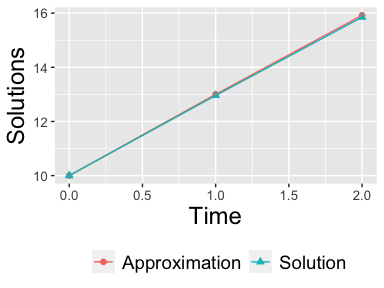
\includegraphics{series_files/figure-latex/eulers_ver1-1.pdf}
\caption{(\#fig:eulers\_ver1)Approximation of a solution using local linearity}
\end{figure}

When you plot them they do look indistinguishable from each other by eye. It looks like we are onto something here!

\hypertarget{defining-an-algorithm}{%
\section{Defining an Algorithm}\label{defining-an-algorithm}}

Here would be an algorithm that would describe our process to determine a solution to a differential equation:

\begin{itemize}
\tightlist
\item
  Determine the locally linear approximation at a given point.
\item
  Forecast out to another time value.
\item
  Repeat the locally linear approximation.
\end{itemize}

If we continue on in this way, let's take a look at how our approximation would do after several days:

\begin{longtable}[]{@{}lll@{}}
\toprule
\(t\) & Approximate Solution & Actual Solution \\
\midrule
\endhead
90 & 118.4 & 117 \\
95 & 119.9 & 118.6 \\
\bottomrule
\end{longtable}

Now it seems that our approximation isn't so accurate as time goes on. What if we updated the infection rate every half day? I know this means that we would be doing additional work (more iterations), but taking smaller timesteps goes hand in hand with more accurate solutions. Let's start out smaller with the first few timesteps:

\begin{longtable}[]{@{}llll@{}}
\toprule
\(t\) & \(I\) & \(\displaystyle \frac{dI}{dt}\) & \(\displaystyle \frac{dI}{dt} \cdot \Delta t\) \\
\midrule
\endhead
0 & 10 & 3 & 1.5 \\
0.5 & = 10 + 1.5 = 11.5 & 2.96 & 1.48 \\
1 & = 11.5 + 1.48 = 12.98 & 2.92 & 1.46 \\
1.5 & = 12.92 + 1.46 = 14.38 & 2.88 & 1.44 \\
2 & = 14.38 + 1.44 = 15.82 & & \\
\bottomrule
\end{longtable}

Notice how we have started to build up a way to organize how to compute the solution. Each column is a ``step'\,' of the method, computing the solution at a new timestep based on our step size \(\Delta t\). The third column just computes the value of the derivative for a particular time and \(I\), and then the fourth column is the \emph{increment} size, or the amount we are forecasting the solution will grow by to the next timestep. (There are other ways to think about this, but if you have a \emph{rate of change } multiplied by a time increment this will give you an approximation to the net change in a function.)

This idea of \emph{approximate, forecast, repeat} is the heart of many \href{https://en.wikipedia.org/wiki/Numerical_methods_for_ordinary_differential_equations}{numerical methods} that approximate solutions to differential equations. The particular method that we have developed here is called \emph{Euler's Method}. We display the results from additional steps in Figure \ref{fig:eulers-ver2}.

\begin{figure}
\centering
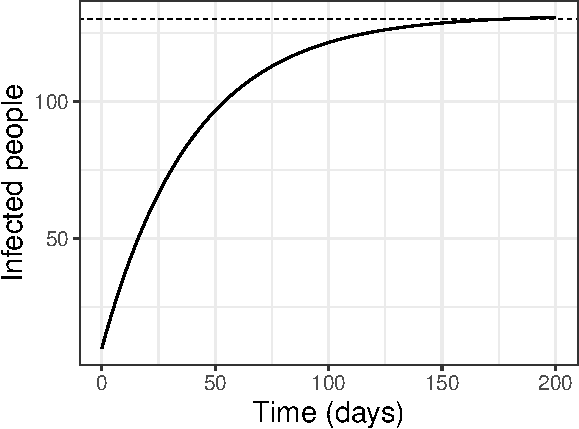
\includegraphics{series_files/figure-latex/eulers-ver2-1.pdf}
\caption{\label{fig:eulers-ver2}Approximation of a solution using local linearity}
\end{figure}

You may notice that the approximation in Figure @ref(fig:eulers\_ver2) compares very favorably to the actual solution function. At the end, we have the following comparisons:

\begin{longtable}[]{@{}
  >{\raggedright\arraybackslash}p{(\columnwidth - 6\tabcolsep) * \real{0.25}}
  >{\raggedright\arraybackslash}p{(\columnwidth - 6\tabcolsep) * \real{0.25}}
  >{\raggedright\arraybackslash}p{(\columnwidth - 6\tabcolsep) * \real{0.25}}
  >{\raggedright\arraybackslash}p{(\columnwidth - 6\tabcolsep) * \real{0.25}}@{}}
\toprule
\(t\) & Euler's Method (\(\Delta t = 1\)) & Euler's Method (\(\Delta t = 0.5\)) & Actual Solution \\
\midrule
\endhead
190 & 130.5 & 129.7 & 129 \\
195 & 130.6 & 129.8 & 129.1 \\
200 & 130.7 & 129.9 & 129.2 \\
\bottomrule
\end{longtable}

There is a tradeoff here - the smaller stepsizes you have the more work it will take to compute you solution. You may have seen a similar tradeoff in Calculus when you explored numerical integration and Riemann sums.

\hypertarget{building-an-iterative-method}{%
\section{Building an iterative method}\label{building-an-iterative-method}}

Now that we have worked on an example, let's carefully formulate Euler's method with another example. Consider the following differential equation:

Consider the following equation that describes the rate of change of the spread of a disease (such as Ebola, as we covered in the first section):

\[ \frac{dI}{dt} = 0.003 I \cdot (4000-I)  \]

Let's call the function \(f(I) = 0.03 I\cdot (4000-I)\). In order to numerically approximate the solution, we will need to recall some concepts from calculus. One way that we can approximate the derivative is through a difference function:

\[ \frac{dI}{dt} = \lim_{\Delta t \rightarrow 0} \frac{I(t+\Delta t) - I(t)}{\Delta t} \]

As long as we consider the quantity \(\Delta t\) to be small (say for this problem 0.1 days if you would like to have units attached to this), we can approximate the derivative with difference function on the right hand side. With this information, we have a reasonable way to organize the problem:

\begin{align*}
\frac{I(t+\Delta t) - I(t)}{\Delta t}  &= 0.003 I \cdot (4000-I) \\
I(t+\Delta t) - I(t)  &= 0.003 I \cdot (4000-I)  \cdot \Delta t \\
I(t+\Delta t) &= I(t) + 0.003 I \cdot (4000-I)  \cdot \Delta t
\end{align*}

The last equation \(I(t+\Delta t) = I(t) + 0.03 I \cdot (4000-I) \cdot \Delta t = f(I) \cdot \Delta t\) is a reasonable way to define an iterative system, especially if we have a spreadsheet program. Here is some code in \texttt{R} that can define a for loop to do this in an iterative way and then plot the solution with \texttt{plotData}:

\begin{Shaded}
\begin{Highlighting}[]
\CommentTok{\# Define your timestep and time vector}
\NormalTok{deltaT }\OtherTok{\textless{}{-}} \FloatTok{0.1}
\NormalTok{t }\OtherTok{\textless{}{-}} \FunctionTok{seq}\NormalTok{(}\DecValTok{0}\NormalTok{,}\DecValTok{2}\NormalTok{,}\AttributeTok{by=}\NormalTok{deltaT)}

\CommentTok{\# Define the number of steps we take.  This is equal to 10 / dt (why?)}
\NormalTok{N }\OtherTok{\textless{}{-}} \FunctionTok{length}\NormalTok{(t)}

\CommentTok{\# Define the initial condition}
\NormalTok{i\_approx }\OtherTok{\textless{}{-}} \DecValTok{10}

\CommentTok{\# Define a vector for your solution:the derivative equation}
\ControlFlowTok{for}\NormalTok{(i }\ControlFlowTok{in} \DecValTok{2}\SpecialCharTok{:}\NormalTok{N) \{  }\CommentTok{\# We start this at 2 because the first value is 10}
\NormalTok{  didt }\OtherTok{\textless{}{-}}\NormalTok{ .}\DecValTok{003} \SpecialCharTok{*}\NormalTok{ i\_approx[i}\DecValTok{{-}1}\NormalTok{] }\SpecialCharTok{*}\NormalTok{ (}\DecValTok{4000}\SpecialCharTok{{-}}\NormalTok{i\_approx[i}\DecValTok{{-}1}\NormalTok{])}
\NormalTok{  i\_approx[i] }\OtherTok{\textless{}{-}}\NormalTok{ i\_approx[i}\DecValTok{{-}1}\NormalTok{] }\SpecialCharTok{+}\NormalTok{ didt}\SpecialCharTok{*}\NormalTok{deltaT}
\NormalTok{\}}


\CommentTok{\# Define your data for the solution into a tibble:}
\NormalTok{solution\_data }\OtherTok{\textless{}{-}} \FunctionTok{tibble}\NormalTok{(}\AttributeTok{time =}\NormalTok{t,}
                        \AttributeTok{infected =}\NormalTok{ i\_approx)}

\CommentTok{\# Now plot your solution:}
\FunctionTok{ggplot}\NormalTok{(}\AttributeTok{data =}\NormalTok{ solution\_data) }\SpecialCharTok{+}
  \FunctionTok{geom\_line}\NormalTok{(}\FunctionTok{aes}\NormalTok{(}\AttributeTok{x=}\NormalTok{time,}\AttributeTok{y=}\NormalTok{infected)) }
\end{Highlighting}
\end{Shaded}

\begin{figure}
\centering
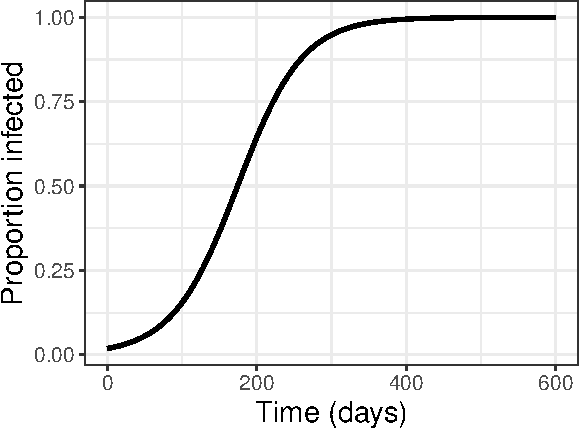
\includegraphics{series_files/figure-latex/my-iterative-method-1.pdf}
\caption{\label{fig:my-iterative-method}An iterative method}
\end{figure}

\begin{Shaded}
\begin{Highlighting}[]
  \FunctionTok{labs}\NormalTok{(}\AttributeTok{x=}\StringTok{\textquotesingle{}Time\textquotesingle{}}\NormalTok{,}
         \AttributeTok{y=}\StringTok{\textquotesingle{}Infected\textquotesingle{}}\NormalTok{)}
\end{Highlighting}
\end{Shaded}

\begin{verbatim}
## $x
## [1] "Time"
## 
## $y
## [1] "Infected"
## 
## attr(,"class")
## [1] "labels"
\end{verbatim}

Ok, let's discuss the different aspects of this code:

\begin{itemize}
\tightlist
\item
  \texttt{deltaT\ \textless{}-\ 0.1} and \texttt{t\ \textless{}-\ seq(0,2,by=deltaT)} define the timesteps (\(\Delta t\)) and the output time vector \texttt{t}. We also define \texttt{N\ \textless{}-\ length(t)} so we know how many steps we take.
\item
  \texttt{i\_approx\ \textless{}-\ 10} defines the initial condition to the system, in other words \(I(0)=10\).
\item
  The for loop goes through this system - first computing the value of \(\displaystyle \frac{dI}{dt}\) and then forecasing out the next timestep \(I(t+\Delta t) = f(I) \cdot \Delta t\)
\item
  The remaining code plots the dataframe, like we learned in Section \ref{r-intro-02}.
\end{itemize}

Let's recap what we've learned to summarize Euler's method. The most general form of a differential equation is:

\[ \displaystyle \frac{d\vec{y}}{dt} = f(\vec{y},\vec{\alpha},t), \]
where \(\vec{y}\) is the vector of state variables you want to solve for, and \(\vec{\alpha}\) is your vector of parameters.

At a given initial condition, Euler's method applies locally linear approximations to forecast the solution forward \(\Delta t\) time units:

\[ \vec{y}_{n+1} = y_{n} + f(\vec{y}_{n},\vec{\alpha},t_{n}) \cdot \Delta t \]

To generate Figure \ref{fig:my-iterative-method} we created the solution directly in R - but you don't want to copy and paste the code. I've created a function called \texttt{euler} that does the same process to generate the output solution:

\begin{Shaded}
\begin{Highlighting}[]
\CommentTok{\# Define the rate equation:}
\NormalTok{system\_eq }\OtherTok{\textless{}{-}} \FunctionTok{c}\NormalTok{(didt }\SpecialCharTok{\textasciitilde{}}\NormalTok{ .}\DecValTok{003} \SpecialCharTok{*}\NormalTok{ i }\SpecialCharTok{*}\NormalTok{ (}\DecValTok{4000}\SpecialCharTok{{-}}\NormalTok{i))}

\CommentTok{\# Define the initial condition (as a named vector)}
\NormalTok{init\_cond }\OtherTok{\textless{}{-}} \FunctionTok{c}\NormalTok{(}\AttributeTok{i=}\DecValTok{10}\NormalTok{)}

\CommentTok{\# Define deltaT and the time steps:}
\NormalTok{deltaT }\OtherTok{=} \FloatTok{0.2}
\NormalTok{n\_steps }\OtherTok{\textless{}{-}} \DecValTok{10}

\CommentTok{\# Compute the solution via Euler\textquotesingle{}s method:}
\NormalTok{out\_solution }\OtherTok{\textless{}{-}} \FunctionTok{euler}\NormalTok{(system\_eq,}\AttributeTok{initial\_condition=}\NormalTok{init\_cond,}\AttributeTok{deltaT=}\NormalTok{deltaT,}\AttributeTok{n\_steps =}\NormalTok{ n\_steps)}


\CommentTok{\# Now plot your solution:}
\FunctionTok{ggplot}\NormalTok{(}\AttributeTok{data =}\NormalTok{ out\_solution) }\SpecialCharTok{+}
  \FunctionTok{geom\_line}\NormalTok{(}\FunctionTok{aes}\NormalTok{(}\AttributeTok{x=}\NormalTok{t,}\AttributeTok{y=}\NormalTok{i)) }
\end{Highlighting}
\end{Shaded}

\begin{figure}
\centering
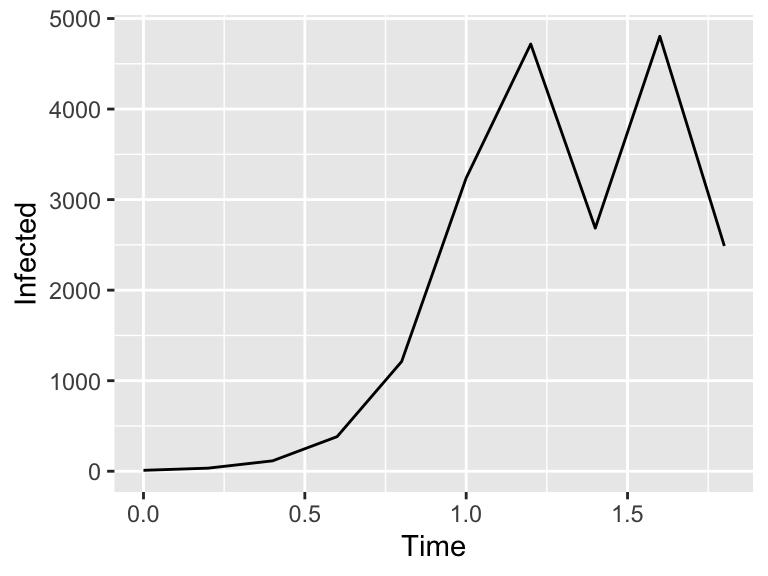
\includegraphics{series_files/figure-latex/unnamed-chunk-63-1.pdf}
\caption{\label{fig:unnamed-chunk-63}Euler's method solution}
\end{figure}

\begin{Shaded}
\begin{Highlighting}[]
  \FunctionTok{labs}\NormalTok{(}\AttributeTok{x=}\StringTok{\textquotesingle{}Time\textquotesingle{}}\NormalTok{,}
         \AttributeTok{y=}\StringTok{\textquotesingle{}Infected\textquotesingle{}}\NormalTok{)}
\end{Highlighting}
\end{Shaded}

\begin{verbatim}
## $x
## [1] "Time"
## 
## $y
## [1] "Infected"
## 
## attr(,"class")
## [1] "labels"
\end{verbatim}

Let's talk through the steps of this code as well:

\begin{itemize}
\tightlist
\item
  The line \texttt{system\_eq\ \textless{}-\ c(didt\ \textasciitilde{}\ .003\ *\ i\ *\ (4000-i))} represents the differential equation, written in formula notation. So \(\displaystyle \frac{dI}{dt} \rightarrow\) \texttt{didt} and \(f(I) \rightarrow\) \texttt{.003\ *\ i\ *\ (4000-i))}, with the variable \texttt{i}.
\item
  The initial condition \(I(0)=10\) is written as a \textbf{named vector:} \texttt{init\_cond\ \textless{}-\ c(i=10)}. Make sure the name of the variable is consistent with your differential equation.
\item
  As before we need to identify \(\Delta t\) and the number of steps \(N\).
\end{itemize}

The command \texttt{euler} then computes the solution applying Euler's method, returning a data frame so we can plot the results. Note the columns of the data frame are the variables \(t\) and \(i\) that have been named in our equations.

\hypertarget{eulers-method-applied-to-systems}{%
\section{Euler's method applied to systems}\label{eulers-method-applied-to-systems}}

Here is a sample code that shows the dynamics for the Lotka-Volterra equations, as studied in Section \ref{modeling-rates-03}:

\begin{equation}
\begin{split} 
\frac{dH}{dt} &= r H - bHL \\  \label{eq:lynx-hare-04}
\frac{dL}{dt} &= e  b  H L - dL
\end{split}
\end{equation}

We are going to use Euler's method to solve this differential equation. Similar to the previous example we will need to determine the f

\begin{Shaded}
\begin{Highlighting}[]
\CommentTok{\# Define the rate equation:}
\NormalTok{system\_eq }\OtherTok{\textless{}{-}} \FunctionTok{c}\NormalTok{(dHdt }\SpecialCharTok{\textasciitilde{}}\NormalTok{ r}\SpecialCharTok{*}\NormalTok{H}\SpecialCharTok{{-}}\NormalTok{b}\SpecialCharTok{*}\NormalTok{H}\SpecialCharTok{*}\NormalTok{L,}
\NormalTok{               dLdt }\SpecialCharTok{\textasciitilde{}}\NormalTok{ e}\SpecialCharTok{*}\NormalTok{b}\SpecialCharTok{*}\NormalTok{H}\SpecialCharTok{*}\NormalTok{L}\SpecialCharTok{{-}}\NormalTok{d}\SpecialCharTok{*}\NormalTok{L)}


\CommentTok{\# Define the parameters (as a named vector)}
\NormalTok{lynx\_hare\_params }\OtherTok{\textless{}{-}} \FunctionTok{c}\NormalTok{(}\AttributeTok{r =} \DecValTok{2}\NormalTok{, }\AttributeTok{b =} \FloatTok{0.5}\NormalTok{, }\AttributeTok{e =} \FloatTok{0.1}\NormalTok{, }\AttributeTok{d =} \DecValTok{1}\NormalTok{)   }\CommentTok{\# parameters: a named vector}

\CommentTok{\# Define the initial condition (as a named vector)}
\NormalTok{init\_cond }\OtherTok{\textless{}{-}} \FunctionTok{c}\NormalTok{(}\AttributeTok{H=}\DecValTok{1}\NormalTok{, }\AttributeTok{L=}\DecValTok{3}\NormalTok{)}

\CommentTok{\# Define deltaT and the time steps:}
\NormalTok{deltaT }\OtherTok{\textless{}{-}} \FloatTok{0.05}    \CommentTok{\# timestep length}
\NormalTok{timeSteps }\OtherTok{\textless{}{-}} \DecValTok{200}   \CommentTok{\# must be a number greater than 1}

\CommentTok{\# Compute the solution via Euler\textquotesingle{}s method:}
\NormalTok{out\_solution }\OtherTok{\textless{}{-}} \FunctionTok{euler}\NormalTok{(system\_eq,}
                      \AttributeTok{parameters =}\NormalTok{ lynx\_hare\_params,}
                      \AttributeTok{initial\_condition=}\NormalTok{init\_cond,}
                      \AttributeTok{deltaT=}\NormalTok{deltaT,}
                      \AttributeTok{n\_steps =}\NormalTok{ n\_steps)}

\CommentTok{\# Make a plot of the solution, using different colors for lynx or hares.}
\FunctionTok{ggplot}\NormalTok{(}\AttributeTok{data =}\NormalTok{ out\_solution) }\SpecialCharTok{+}
  \FunctionTok{geom\_line}\NormalTok{(}\FunctionTok{aes}\NormalTok{(}\AttributeTok{x=}\NormalTok{t,}\AttributeTok{y=}\NormalTok{H),}\AttributeTok{color=}\StringTok{\textquotesingle{}red\textquotesingle{}}\NormalTok{) }\SpecialCharTok{+}
  \FunctionTok{geom\_line}\NormalTok{(}\FunctionTok{aes}\NormalTok{(}\AttributeTok{x=}\NormalTok{t,}\AttributeTok{y=}\NormalTok{L),}\AttributeTok{color=}\StringTok{\textquotesingle{}blue\textquotesingle{}}\NormalTok{) }\SpecialCharTok{+}
\FunctionTok{labs}\NormalTok{(}\AttributeTok{x=}\StringTok{\textquotesingle{}Time\textquotesingle{}}\NormalTok{,}
     \AttributeTok{y=}\StringTok{\textquotesingle{}Lynx (red) or Hares (blue)\textquotesingle{}}\NormalTok{)}
\end{Highlighting}
\end{Shaded}

\begin{figure}
\centering
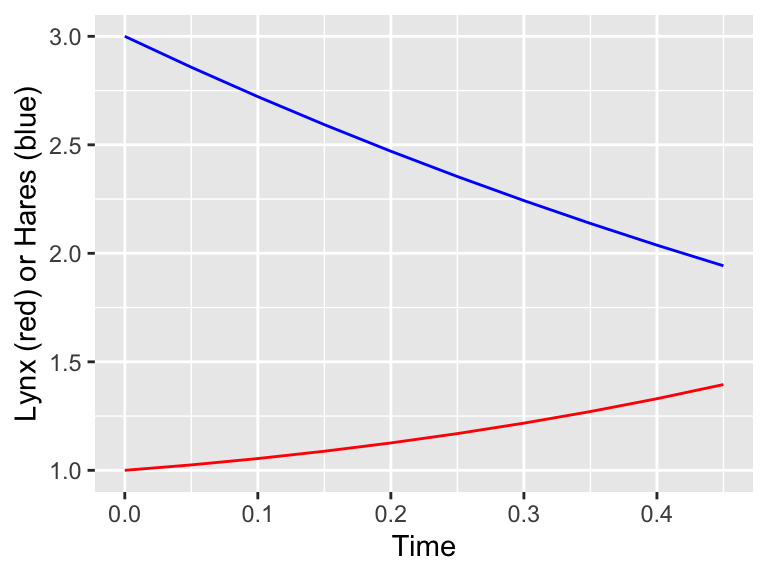
\includegraphics{series_files/figure-latex/unnamed-chunk-64-1.pdf}
\caption{\label{fig:unnamed-chunk-64}Euler's method solution for Lynx-Hare system}
\end{figure}

This example is structured similarly as a single variable differential equation, with some key changes:

\begin{itemize}
\tightlist
\item
  The variable \texttt{system\_eq} is now a vector, with each entry one of the rate equations.
\item
  We need to identify both variables in their initial condition.
\item
  Most importantly, Equation \eqref{eq:lynx-hare-04} has parameters, which we define as a named vector \texttt{lynx\_hare\_params\ \textless{}-\ c(r\ =\ 2,\ b\ =\ 0.5,\ e\ =\ 0.1,\ d\ =\ 1)} that we pass through to the command \texttt{euler} with the option \texttt{parameters}. If your equation does not have any parameters you do not need to worry about it.
\item
  We plot both solutions together at the end, or you can make two separate plots. Remember that you can choose the color in your plot.
\end{itemize}

Thankfully the code is pretty easy to adapt for systems of equations!

\hypertarget{more-refined-numerical-solvers}{%
\section{More refined numerical solvers}\label{more-refined-numerical-solvers}}

Perhaps in the course of working with Euler's method you encounter a differential equation that produces some nonsensible results. Take for example the following which is the implementation of our quarantine model:

\begin{Shaded}
\begin{Highlighting}[]
\NormalTok{system\_eq }\OtherTok{\textless{}{-}} \FunctionTok{c}\NormalTok{(dSdt }\SpecialCharTok{\textasciitilde{}} \SpecialCharTok{{-}}\NormalTok{k}\SpecialCharTok{*}\NormalTok{S}\SpecialCharTok{*}\NormalTok{I,}
\NormalTok{               dIdt }\SpecialCharTok{\textasciitilde{}}\NormalTok{ k}\SpecialCharTok{*}\NormalTok{S}\SpecialCharTok{*}\NormalTok{I}\SpecialCharTok{{-}}\NormalTok{beta}\SpecialCharTok{*}\NormalTok{I)}


\NormalTok{deltaT }\OtherTok{\textless{}{-}}\NormalTok{ .}\DecValTok{1}    \CommentTok{\# timestep length}
\NormalTok{timeSteps }\OtherTok{\textless{}{-}} \DecValTok{15}   \CommentTok{\# must be a number greater than 1}

\NormalTok{quarantine\_parameters }\OtherTok{\textless{}{-}} \FunctionTok{c}\NormalTok{(}\AttributeTok{k=}\NormalTok{.}\DecValTok{05}\NormalTok{, }\AttributeTok{beta=}\NormalTok{.}\DecValTok{2}\NormalTok{)   }\CommentTok{\# parameters: a named vector}

\NormalTok{init\_cond }\OtherTok{\textless{}{-}} \FunctionTok{c}\NormalTok{(}\AttributeTok{S=}\DecValTok{300}\NormalTok{, }\AttributeTok{I=}\DecValTok{1}\NormalTok{)  }\CommentTok{\# Be sure you have enough conditions as you do variables.}

\CommentTok{\# Compute the solution via Euler\textquotesingle{}s method:}
\NormalTok{out\_solution }\OtherTok{\textless{}{-}} \FunctionTok{euler}\NormalTok{(system\_eq,}
                      \AttributeTok{parameters =}\NormalTok{ quarantine\_parameters,}
                      \AttributeTok{initial\_condition=}\NormalTok{init\_cond,}
                      \AttributeTok{deltaT=}\NormalTok{deltaT,}
                      \AttributeTok{n\_steps =}\NormalTok{ n\_steps)}


\FunctionTok{ggplot}\NormalTok{(}\AttributeTok{data =}\NormalTok{ out\_solution) }\SpecialCharTok{+}
  \FunctionTok{geom\_line}\NormalTok{(}\FunctionTok{aes}\NormalTok{(}\AttributeTok{x=}\NormalTok{t,}\AttributeTok{y=}\NormalTok{S),}\AttributeTok{color=}\StringTok{\textquotesingle{}red\textquotesingle{}}\NormalTok{) }\SpecialCharTok{+}
  \FunctionTok{geom\_line}\NormalTok{(}\FunctionTok{aes}\NormalTok{(}\AttributeTok{x=}\NormalTok{t,}\AttributeTok{y=}\NormalTok{I),}\AttributeTok{color=}\StringTok{\textquotesingle{}blue\textquotesingle{}}\NormalTok{) }\SpecialCharTok{+}
  \FunctionTok{labs}\NormalTok{(}\AttributeTok{x=}\StringTok{\textquotesingle{}Time\textquotesingle{}}\NormalTok{,}
       \AttributeTok{y=}\StringTok{\textquotesingle{}Susceptible (red) or Infected (blue)\textquotesingle{}}\NormalTok{)}
\end{Highlighting}
\end{Shaded}

\begin{figure}
\centering
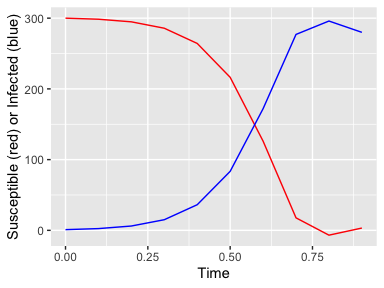
\includegraphics{series_files/figure-latex/unnamed-chunk-65-1.pdf}
\caption{\label{fig:unnamed-chunk-65}Surprising results with Euler's method.}
\end{figure}

You may notice the solution for \(S\) wiggles around \(t=0.75\) and is negative. This is concerning because we know there can't be negative people! This requires a little more investigation.

If we take a look at \(t=0.75\) the value for \(S \approx 1\) and the value for \(I \approx 280\). If we let \(k=0.05\) and \(\beta=0.2\), this means that \(\displaystyle \frac{dS}{dt}=-14\) and \(\displaystyle \frac{dI}{dt}=-42\). The values of \(S\) and \(I\) are both decreasing! We know that our Euler's method update is one where the new value is the old value plus any change. So the new value for \(S = 1 -14\cdot 0.1 = -0.4\). Mathematically Euler's method is doing nothing incorrect, but we know realistically this cannot happen.

In turns out that this can easily be overcome. While Euler's method is useful, it does quite poorly in cases where the solution is changing rapidly - or we might need to make some smaller step sizes. How we remedy this is to use a \emph{higher order solver}, and one such method is called the \href{https://en.wikipedia.org/wiki/Runge\%E2\%80\%93Kutta_methods}{Runge-Kutta Method}. If you take a course in numerical analysis you might study these, but for the moment you see the difference between the twoa Runge-Kutta solver implemented in the \texttt{demodelr} package, which by all intents and purposes is replaces the command \texttt{euler} with \texttt{rk4}:

\begin{Shaded}
\begin{Highlighting}[]
\NormalTok{system\_eq }\OtherTok{\textless{}{-}} \FunctionTok{c}\NormalTok{(dSdt }\SpecialCharTok{\textasciitilde{}} \SpecialCharTok{{-}}\NormalTok{k}\SpecialCharTok{*}\NormalTok{S}\SpecialCharTok{*}\NormalTok{I,}
\NormalTok{               dIdt }\SpecialCharTok{\textasciitilde{}}\NormalTok{ k}\SpecialCharTok{*}\NormalTok{S}\SpecialCharTok{*}\NormalTok{I}\SpecialCharTok{{-}}\NormalTok{beta}\SpecialCharTok{*}\NormalTok{I)}


\NormalTok{deltaT }\OtherTok{\textless{}{-}}\NormalTok{ .}\DecValTok{1}    \CommentTok{\# timestep length}
\NormalTok{timeSteps }\OtherTok{\textless{}{-}} \DecValTok{15}   \CommentTok{\# must be a number greater than 1}

\NormalTok{quarantine\_parameters }\OtherTok{\textless{}{-}} \FunctionTok{c}\NormalTok{(}\AttributeTok{k=}\NormalTok{.}\DecValTok{05}\NormalTok{, }\AttributeTok{beta=}\NormalTok{.}\DecValTok{2}\NormalTok{)   }\CommentTok{\# parameters: a named vector}

\NormalTok{init\_cond }\OtherTok{\textless{}{-}} \FunctionTok{c}\NormalTok{(}\AttributeTok{S=}\DecValTok{300}\NormalTok{, }\AttributeTok{I=}\DecValTok{1}\NormalTok{)  }\CommentTok{\# Be sure you have enough conditions as you do variables.}

\CommentTok{\# Compute the solution via a Runge{-}Kutta method:}
\NormalTok{out\_solution }\OtherTok{\textless{}{-}} \FunctionTok{rk4}\NormalTok{(system\_eq,}
                      \AttributeTok{parameters =}\NormalTok{ quarantine\_parameters,}
                      \AttributeTok{initial\_condition=}\NormalTok{init\_cond,}
                      \AttributeTok{deltaT=}\NormalTok{deltaT,}
                      \AttributeTok{n\_steps =}\NormalTok{ n\_steps)}


\FunctionTok{ggplot}\NormalTok{(}\AttributeTok{data =}\NormalTok{ out\_solution) }\SpecialCharTok{+}
  \FunctionTok{geom\_line}\NormalTok{(}\FunctionTok{aes}\NormalTok{(}\AttributeTok{x=}\NormalTok{t,}\AttributeTok{y=}\NormalTok{S),}\AttributeTok{color=}\StringTok{\textquotesingle{}red\textquotesingle{}}\NormalTok{) }\SpecialCharTok{+}
  \FunctionTok{geom\_line}\NormalTok{(}\FunctionTok{aes}\NormalTok{(}\AttributeTok{x=}\NormalTok{t,}\AttributeTok{y=}\NormalTok{I),}\AttributeTok{color=}\StringTok{\textquotesingle{}blue\textquotesingle{}}\NormalTok{) }\SpecialCharTok{+}
  \FunctionTok{labs}\NormalTok{(}\AttributeTok{x=}\StringTok{\textquotesingle{}Time\textquotesingle{}}\NormalTok{,}
       \AttributeTok{y=}\StringTok{\textquotesingle{}Susceptible (red) or Infected (blue)\textquotesingle{}}\NormalTok{)}
\end{Highlighting}
\end{Shaded}

\begin{figure}
\centering
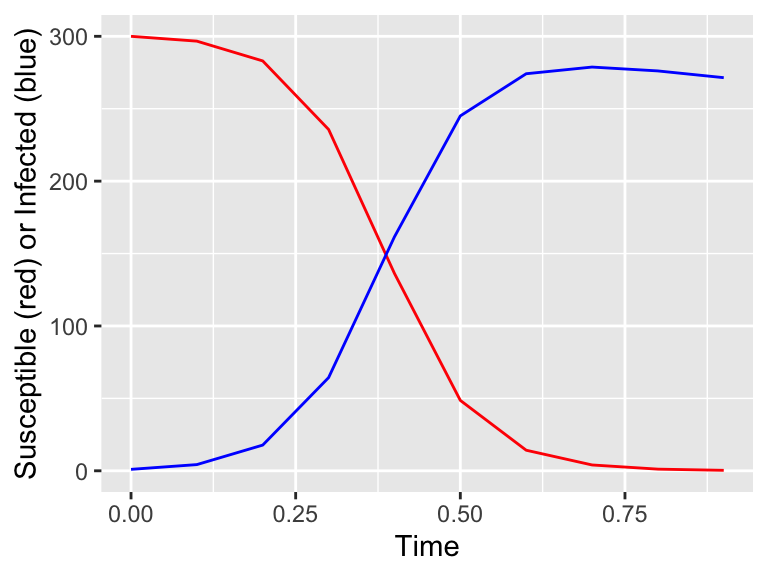
\includegraphics{series_files/figure-latex/unnamed-chunk-66-1.pdf}
\caption{\label{fig:unnamed-chunk-66}Better results with the Runge-Kutta method.}
\end{figure}

So what is going on here? Briefly, the differences between the two methods have to do with the error in the numerical method. The error is quantified as the difference between the actual solution and the numerical solution. Euler's method has an error on the order of the stepsize \(\Delta t\), whereas the Runge-Kutta method has an error of \((\Delta t)^4\). For this example \(\Delta t = .1\), so \((\Delta t)^{4} =.0001\) - that is a noticeable difference! We can improve Euler's method by taking a smaller timestep - BUT that means we need a larger number of steps \(N\) - which may take more computational time.

Does this discussion sound familiar? Perhaps you examined similar when you took calculus and studied Riemann sums to approximate the area underneath a curve (left sum, right sum, trapezoid, midpoint). It turns out that these two problems are closely related. Numerical analysis is a great field of study to examine these topics and others!

Moving ahead, I might switch between Euler's method or the Runge-Kutta method when solving a differential equation. Thankfully the bulk of the work is ``under the hood'' - the setup will be the same for both!

\newpage

\hypertarget{exercises-3}{%
\section{Exercises}\label{exercises-3}}

\begin{exercise}
\protect\hypertarget{exr:unnamed-chunk-67}{}{\label{exr:unnamed-chunk-67} }Verify that \(I(t) = 130-120e^{-0.25t}\) is a solution to the differential equation \[\displaystyle \frac{dI}{dt} = 130-0.025I \] with \(I(0)=10\).
\end{exercise}

~

\begin{exercise}
\protect\hypertarget{exr:unnamed-chunk-68}{}{\label{exr:unnamed-chunk-68} }Apply the \texttt{rk4} solver with \(\Delta t = 0.1\) with \(N=10\) to the initial value problem \(\displaystyle \frac{dI}{dt} = 0.003 I \cdot (4000-I) \; I(0)=10\). Compare your graph to Figure \ref{fig:my-iterative-method}. What differences do you observe? Which solution method (\texttt{euler} or \texttt{rk4}) is better (and why)?
\end{exercise}

~

\begin{exercise}
\protect\hypertarget{exr:unnamed-chunk-69}{}{\label{exr:unnamed-chunk-69} }The following exercise will help you explore the relationships between stepsize, ending points, and number of steps needed. You may assume that we will start at \(t=0\) in all parts.

\begin{enumerate}[label=\alph*.]
\item If we wish to do an Euler's method solution with step size 1 second and ending at $t=5$ seconds, how many steps will we take?
\item If we wish to do an Euler's method solution with step size 0.5 seconds and ending at $t=5$ seconds, how many steps will we take?
\item If we wish to do an Euler's method solution with step size 0.1 seconds and ending at $t=5$ seconds, how many steps will we take?
\item If we wish to do an Euler's method solution with step size $\Delta t$ and go to ending value of $T$, what is an expression that relates the number steps $N$ as a function of $\Delta t$ and $T$?
\end{enumerate}
\end{exercise}

~

\begin{exercise}
\protect\hypertarget{exr:unnamed-chunk-70}{}{\label{exr:unnamed-chunk-70} }To get a rough approximation between error and step size, let's say for a particular differential equation that we are starting at \(t=0\) and going to \(t=2\), with \(\Delta t = 0.2\). We know that the Runge-Kutta error will be on the order of \((\Delta t)^{4} =0.0016\). If we want to use Euler's method with the same order of error, we could say \(\Delta t = .0001\). For that case, how many steps will we need to take?
\end{exercise}

~

\begin{exercise}
\protect\hypertarget{exr:euler-solve}{}{\label{exr:euler-solve} }For each of the following differential equations, apply Euler's method to generate a numerical solution to the differential equation and plot your solution. The stepsize (\(\Delta t\)) and number of iterations (\(N\)) are listed.

\begin{enumerate}[label=\alph*.]
\item Differential equation: $\displaystyle \frac{dS}{dt} =3-S$. Set $\Delta t = 0.1$, $N = 50$. Initial conditions:  $S(0) = 0.5$, $S(0) = 5$.
\item Differential Equation: $\displaystyle \frac{dS}{dt} =\frac{1}{1-S}$. Set $\Delta t = 0.01$, $N = 30$. Initial conditions:  $S(0) = 0.5$, $S(0) = 2$.
\item Differential equation: $\displaystyle \frac{dS}{dt} = 0.8 \cdot S \cdot (10-S)$. Set $\Delta t = 0.1$, $N = 50$. Initial conditions:  $S(0) = 3$, $S(0) = 10$.
\end{enumerate}
\end{exercise}

~

\begin{exercise}
\protect\hypertarget{exr:unnamed-chunk-71}{}{\label{exr:unnamed-chunk-71} }For each of the following differential equations, apply the Runge-Kutta method method to generate a numerical solution to the differential equation and plot your solution. The stepsize (\(\Delta t\)) and number of iterations (\(N\)) are listed. Contrast your answers with Exercise \ref{exr:euler-solve}.

\begin{enumerate}[label=\alph*.]
\item Differential equation: $\displaystyle \frac{dS}{dt} =3-S$. Set $\Delta t = 0.1$, $N = 50$. Initial conditions:  $S(0) = 0.5$, $S(0) = 5$.
\item Differential Equation: $\displaystyle \frac{dS}{dt} =\frac{1}{1-S}$. Set $\Delta t = 0.01$, $N = 30$. Initial conditions:  $S(0) = 0.5$, $S(0) = 2$.
\item Differential equation: $\displaystyle \frac{dS}{dt} = 0.8 \cdot S \cdot (10-S)$. Set $\Delta t = 0.1$, $N = 50$. Initial conditions:  $S(0) = 3$, $S(0) = 10$.
\end{enumerate}
\end{exercise}

~

\begin{exercise}
\protect\hypertarget{exr:unnamed-chunk-72}{}{\label{exr:unnamed-chunk-72} }Let's do some more work with Euler's method for \(\displaystyle \frac{dS}{dt} = 0.8 \cdot S \cdot (10-S)\). This time set \(S(0)=15\), \(\Delta t = 0.1\), \(N = 10\).
When you examine your solution, what is incorrect about the Euler's method solution based on your qualitative knowledge of the underlying dynamics? Now calculate Euler's method for the same differential equation for the following conditions: \(S(0)=15\), \(\Delta t = 0.01\), \(N = 100\). What has changed in your solution?
\end{exercise}

~

\begin{exercise}
\protect\hypertarget{exr:euler-ftbu}{}{\label{exr:euler-ftbu} }Let's do some more work with Euler's method for \(\displaystyle \frac{dS}{dt} =\frac{1}{1-S}\). This time set \(S(0)=1.5\), \(\Delta t = 0.1\), \(N = 10\) and also \(S(0)=1.5\), \(\Delta t = 0.01\), \(N = 100\). Between these two solutions, what has changed? Do you think it is numerically possible to calculate a reasonable solution for Euler's method near \(S=1\)? (\emph{note: this differential equation is an example of finite time blow up})
\end{exercise}

~

\begin{exercise}
\protect\hypertarget{exr:rk-ftbu}{}{\label{exr:rk-ftbu} }Similar to Exercise \ref{exr:euler-ftbu}, let's apply the \texttt{rk4} method for \(\displaystyle \frac{dS}{dt} =\frac{1}{1-S}\). This time set \(S(0)=1.5\), \(\Delta t = 0.1\), \(N = 10\) and also \(S(0)=1.5\), \(\Delta t = 0.01\), \(N = 100\). Between these two solutions, what has changed? Does this numerical solver do a better job in computing solutions compared to the Euler method? (\emph{note: this differential equation is an example of finite time blow up})
\end{exercise}

~

\begin{exercise}
\protect\hypertarget{exr:unnamed-chunk-73}{}{\label{exr:unnamed-chunk-73} }One way to model the growth rate hares is with \(\displaystyle f(H) = \frac{r H}{1+kH}\), where \(r\) and \(k\) are parameters. This is in constrast to exponential growth, which assumes \(f(H) = rH\).

\begin{enumerate}[label=\alph*.]
\item First evaluate $\displaystyle \lim_{H \rightarrow \infty} rH$.
\item Then $\displaystyle \lim_{H \rightarrow \infty} \frac{r H}{1+kH}$.
\item Compare your two answers. Discuss how the growth rate $\displaystyle f(H) = \frac{r H}{1+kH}$ seems to be a more realistic model.
\end{enumerate}
\end{exercise}

~
\begin{exercise}
\protect\hypertarget{exr:unnamed-chunk-74}{}{\label{exr:unnamed-chunk-74} }In the lynx hare example we can also consider an alternative system where the growth of the hare is not exponential:

\begin{equation}
\begin{split}
\frac{dH}{dt} &= \frac{2 H}{1+kH} - 0.5HL \\ 
\frac{dL}{dt} &= 0.05  H L - dL
\end{split}
\end{equation}

Set the number of timesteps to be 2000. Apply Euler's method to numerically solve this system of equations when \(k=0.1\) and \(k=1\). Plot your simulation results.
\end{exercise}
~

For the following differential equations use the code \texttt{euler} to generate a numerical solution to the differential equation and plot your solution. The stepsize (\(\Delta t\)) and number of iterations (\(N\)) are listed. After your Euler's method solution is determined, explain why you would expect the behavior in the solution that you see.

\begin{exercise}
\protect\hypertarget{exr:unnamed-chunk-75}{}{\label{exr:unnamed-chunk-75} }Consider the following:

\begin{itemize}
\item Differential equation: $\displaystyle \frac{dS}{dt} = r \cdot S \cdot (K-S) $.
\item Set $r=1.2$ and $K=3$.
\item Set $\Delta t = 0.1$, $N = 50$.
\end{itemize}

\begin{enumerate}[label=\alph*.]
\item Use the code `euler` to generate a numerical solution to the differential equation for the following initial conditions:  $S(0) = 1$, $S(0) = 3$, $S(0) = 5$. 
\item Plot your Euler's method solutions with the three initial conditions on the same plot.  What do you notice when you do plot them together?
\item Make a hypothesis regarding the long term behavior of this system. Then plot a few more solution curves to verify your guess.
\end{enumerate}
\end{exercise}

~

\begin{exercise}
\protect\hypertarget{exr:unnamed-chunk-76}{}{\label{exr:unnamed-chunk-76} }Consider the following:

\begin{itemize}
\item Differential equation: $\displaystyle \frac{dS}{dt} =K-S $.
\item Set $K=2$.
\item Set $\Delta t = 0.1$, $N = 50$.
\end{itemize}

\begin{enumerate}[label=\alph*.]
\item Use the code `euler` to generate a numerical solution to the differential equation for the following initial conditions:  $S(0) = 0$, $S(0) = 2$, $S(0) = 5$. 
\item Plot your Euler's method solutions with the three initial conditions on the same plot.  What do you notice when you do plot them together?
\item Make a hypothesis regarding the long term behavior of this system. Then plot a few more solution curves to verify your guess.
\end{enumerate}
\end{exercise}

\begin{exercise}
\protect\hypertarget{exr:unnamed-chunk-77}{}{\label{exr:unnamed-chunk-77} }Consider the differential equation \(\displaystyle \frac{dS}{dt} = \frac{1}{1-S}\). Notice that at \(S=1\) the rate \(\displaystyle \frac{dS}{dt}\) is not defined.

\begin{enumerate}[label=\alph*.]
\item If you applied Euler's method solution with initial condition $S(0)=0.9$, what do you think your solution would approach as the number of timesteps increased?
\item If you applied Euler's method solution with initial condition $S(0)=1.1$, what do you think your solution would approach as the number of timesteps increased?
\item Explain how you could come to the same conclusion as the previous two problems if you graphed $\displaystyle f(S) = \frac{1}{1-S}$.
\end{enumerate}
\end{exercise}

~

\hypertarget{phase-05}{%
\chapter{Phase lines and equilibrium solutions}\label{phase-05}}

In modeling with differential equations, we want to understand how a system develops both qualitatively and quantitatively. Euler's method (and other associated numerical methods for solving differential equations) illustrate solution behavior numerically. One key thing about the qualitative analysis is we are interested in the \emph{motion} or the ``flow'' of the solution at a given point. Is the solution increasing, decreasing, or staying the same?

For this section we will discuss qualitative aspects of a differential equation. We are going to focus on differential equations in one variable. Section \ref{coupled-06} will build your understanding of the same idea with coupled systems of equations.

\hypertarget{equilibrium-solutions}{%
\section{Equilibrium solutions}\label{equilibrium-solutions}}

A great place to start is where the rate of change for a differential equation is zero, or in other words there is \emph{no} flow. Borrowing ideas from calculus, this occurs when the rate of change is zero. We solve this by setting the left hand side of \(\displaystyle \frac{dy}{dt}=f(y)\) equal to zero and solving for \(y\) (or whatever dependent variable describes the problem).

\begin{example}
\protect\hypertarget{exm:unnamed-chunk-78}{}{\label{exm:unnamed-chunk-78} }What are the equilibrium solutions to \(\displaystyle \frac{dy}{dt}=- y\)?
\end{example}

\begin{solution}
\iffalse{} {Solution. } \fi{}For this example we know that when the rate of change is zero, this means that \(\displaystyle \frac{dy}{dt} = 0\), or when \(0 = -y\). So \(y=0\) is the equilibrium solution.
\end{solution}

The general solution to the differential equation \(\displaystyle \frac{dy}{dt}=- y\) is when \(y(t)=Ce^{-t}\), where \(C\) is an arbitrary constant. Figure \ref{fig:exponential} plots different solution curves, with the equilibrium solution shown as a horizontal line:

\begin{figure}
\centering
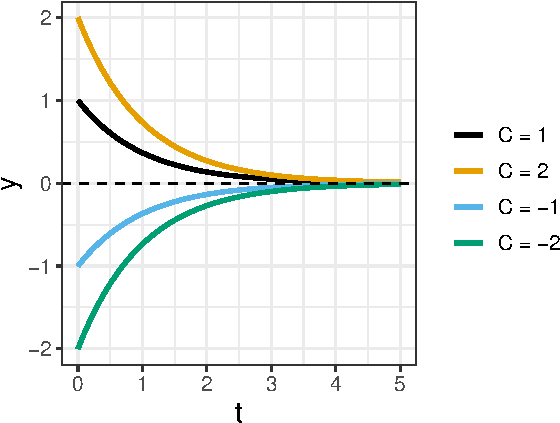
\includegraphics{series_files/figure-latex/exponential-1.pdf}
\caption{\label{fig:exponential}Exponential solution curves}
\end{figure}

Notice that as \(t\) increases, all solutions approach the equilbrium solution \(y=0\) as \(t\) no matter if the initial condition is positive or negative. You can also evaluate the following limit for the solution: \(\displaystyle \lim_{t\rightarrow \infty} Ce^{-t} = 0\) to verify this is the case too.

\begin{example}
\protect\hypertarget{exm:unnamed-chunk-80}{}{\label{exm:unnamed-chunk-80} }What are the equilibrium solutions to \(\displaystyle \frac{dN}{dt} = N \cdot(1-N)\)?
\end{example}

\begin{solution}
\iffalse{} {Solution. } \fi{}In this case the equilibrium solutions occur when \(N \cdot(1-N) = 0\), or when \(N=0\) or \(N=1\).
\end{solution}

The generic solution to this differential equation is \[ \displaystyle N(t)= \frac{N_0}{N_0 +(1-N_0) e^{-t}}.\] Figure \ref{fig:logistic-soln} displays several different solution curves.

\begin{figure}
\centering
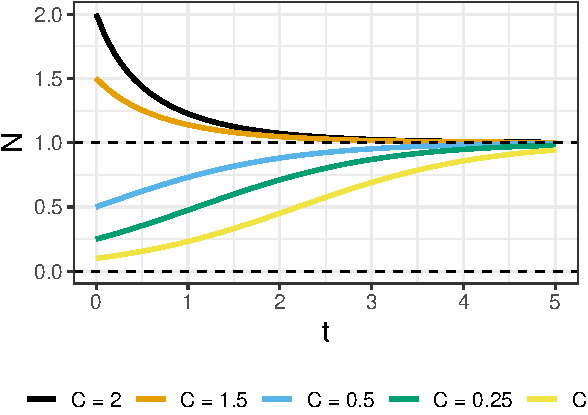
\includegraphics{series_files/figure-latex/logistic-soln-1.pdf}
\caption{\label{fig:logistic-soln}Solution curves for \(N'=N(1-N)\)}
\end{figure}

~

In Figure \ref{fig:logistic-soln} notice how all the solutions tend towards \(N=1\), but even solutions that start close to \(N=0\) seem to move away from this equilibrium solution. This example brings us to understanding classifying the \emph{stability} of the equilibrium solutions.

\hypertarget{phase-lines-for-differentail-equations}{%
\section{Phase lines for differentail equations}\label{phase-lines-for-differentail-equations}}

While it is one thing to determine where the equilibrium solutions are, we are also interested in classifying the \textbf{stability} of the equilibrium solutions. To do this investigate the behavior of the differential around the equilibrium solutions, using facts from calculus:

\begin{itemize}
\tightlist
\item
  If \(\displaystyle \frac{dy}{dt}<0\), the function is decreasing.
\item
  If \(\displaystyle \frac{dy}{dt}>0\), the function is increasing.
\end{itemize}

We say that the solution \(y=0\) is a \emph{stable} equilibrium solution in this case.

Let's apply this logic to our differential equation \(\displaystyle \frac{dy}{dt}=- y\). We know that if \(y=3\), \(\displaystyle \frac{dy}{dt}=- 3 <0\), so we say the function is \emph{decreasing} to \(y=0\). If \(y=-2\), \(\displaystyle \frac{dy}{dt}=- (-2) = 2 >0\), so we say the function is \emph{increasing} to \(y=0\). This can be represented neatly in the phase line diagram for Figure \ref{fig:phaseline1}:

\begin{figure}
\centering
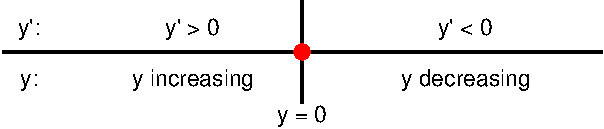
\includegraphics{series_files/figure-latex/phaseline1-1.pdf}
\caption{\label{fig:phaseline1}Phase line to \(y'=-y\).}
\end{figure}

Because the solution is \emph{increasing} to \(y=0\) when \(y <0\), and \emph{decreasing} to \(y=0\) when \(y >0\), we say that the equilibrium solution is \textbf{stable}, which is also confirmed by the solutions we plotted above.

\begin{example}
\protect\hypertarget{exm:general-exponential}{}{\label{exm:general-exponential} }Classify the stability of the equilibrium solutions to \(\displaystyle \frac{dy}{dt} = k \cdot y\), where \(k\) is a parameter.
\end{example}

\begin{solution}
\iffalse{} {Solution. } \fi{}In this case the equilibrium solution is still \(y=0\). We will need to consider two different cases for the stability depending on the value of \(k\) (\(k>0\), \(k<0\), and \(k=0\)):

\begin{itemize}
\tightlist
\item
  When \(k<0\), the phase line will be similar Figure \ref{fig:phaseline1}.
\item
  When \(k>0\) the phase line will be is shown in the Figure \ref{fig:phaseline2}. We say in this case that the equilibrium solution is \emph{unstable}, as all solutions flow away from the equilibrium. Several different solutions are shown in Figure \ref{fig:solncurve-1}
\item
  When \(k=0\) we have the differential equation \(\displaystyle \frac{dy}{dt}=0\), which has \(y=C\) as a general solution. For this special case the equilibrium solution is neither stable or unstable\footnote{By all intents and purposes this is a different differential equation than \(\displaystyle \frac{dy}{dt}=k\cdot y\); something peculiar is going on here - which we come back to when discuss bifurcations in Section \ref{bifurcation-19}.}.
\end{itemize}
\end{solution}

\begin{figure}
\centering
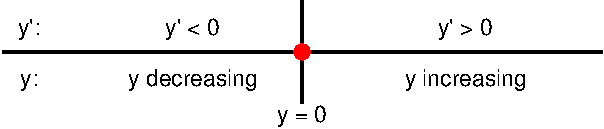
\includegraphics{series_files/figure-latex/phaseline2-1.pdf}
\caption{\label{fig:phaseline2}Phaseline for \(y'=ky\), with \(k>0\).}
\end{figure}

\begin{figure}
\centering
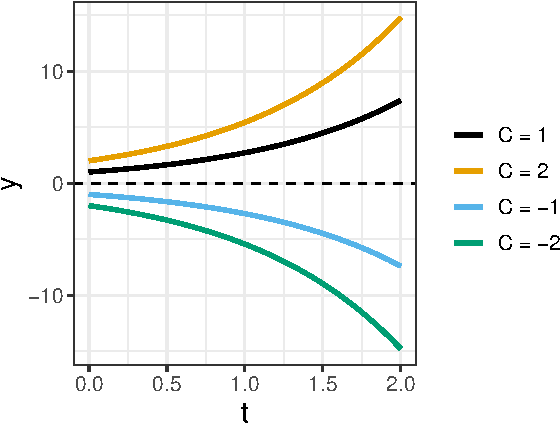
\includegraphics{series_files/figure-latex/solncurve-1-1.pdf}
\caption{\label{fig:solncurve-1}Solution curves for \(y'=ky\), with \(k>0\).}
\end{figure}

~

\begin{example}
\protect\hypertarget{exm:unnamed-chunk-83}{}{\label{exm:unnamed-chunk-83} }Let's investigate the phase line for the differential equation \(\displaystyle \frac{dN}{dt} = N \cdot(1-N)\) and classify stability of the equilibrium solutions.
\end{example}

\begin{solution}
\iffalse{} {Solution. } \fi{}This differential equation has equilbrium solutions when \(N(1-N)=0\), or \(N=0\) or \(N=1\). We evaluate the stability of the solutions in the following table:

\begin{longtable}[]{@{}lll@{}}
\toprule
\textbf{Test point} & \textbf{Sign of \(N'\)} & \textbf{Tendency of solution} \\
\midrule
\endhead
\(N=-1\) & Negative & Decreasing \\
\(N=0\) & Zero & Equilibrium solution \\
\(N=0.5\) & Positive & Increasing \\
\(N=1\) & Zero & Equilibrium solution \\
\(N=2\) & Negative & Decreasing \\
\bottomrule
\end{longtable}

Notice how the selected test points in the first column are either the the \emph{left} or the \emph{right} of the equilbrium solution. We can also represent the information in the table using a phase line diagram (Figure \ref{fig:phaseline-N}), but in this case we need to include \emph{two} equilibrium solutions.

The table and Figure \ref{fig:phaseline-N} confirms that \(N\) is moving \emph{away} from \(N=0\) (either decreasing when \(N\) is less than 0 and increasing when \(N\) is greater than 0) and moving \emph{towards} \(N=1\) (either increasing when \(N\) is between 0 and 1 and decreasing when \(N\) is greater than one.

~
These results suggest that equilibrium solution at \(N=0\) to be \emph{unstable} and at \(N=1\) to be \emph{stable}.
\end{solution}

\begin{figure}
\centering
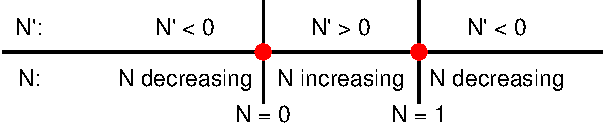
\includegraphics{series_files/figure-latex/phaseline-N-1.pdf}
\caption{\label{fig:phaseline-N}Phase line diagram for the differential equation \(N'=N(1-N)\).}
\end{figure}

Other than writing the words in the phase line diagram, we also use arrows to signify increasing or decreasing in the solutions.

\hypertarget{a-stability-test-for-equilibrium-solutions}{%
\section{A stability test for equilibrium solutions}\label{a-stability-test-for-equilibrium-solutions}}

Notice how when constructing the phase line diagram we relied on the behavior of solutions \emph{around} the equilibrium solution to classify the stability. As an alternative we can also use the point at the equilibrium solution itself.

To do this we are going to consider the general differential equation \(\displaystyle \frac{dy}{dt}=f(y)\). We are going to assume that we have an equilibrium solution at \(y=y_{*}\).

We use local linearization to construct a locally linear approximation to \(L(y)\) to \(f(y)\) at \(y=y_{*}\):

\[L(y) = f(y_{*}) + f'(y_{*}) \cdot (y-y_{*})  \]
We will use \(L(y)\) as an approximation to \(f(y)\). There are two key things here. First, because we have an equilibrium solution, \(f(y_{*}) =0\). The other key thing is that if we define the variable \(P = y-y_{*}\), then the differential equation translates to

\begin{equation}
\frac{dP}{dt} = f'(y_{*}) \cdot P  \label{eq:local-linear}
\end{equation}

Does Equation \eqref{eq:local-linear} look familiar? I - it should! This is similar to the example where we classified the stability of \(\displaystyle \frac{dy}{dt} = k \cdot y\) -- cool! So let's use what we learned in Example \ref{exm:general-exponential} above to classify the stability:

\textbf{Local linearization stability test for equilibrium solutions:} For a differential equation \(\displaystyle \frac{dy}{dt} = f(y)\) with equilibrium solution \(y_{*}\), we can classify the stability of the equilibrium solution through the following:

\begin{itemize}
\tightlist
\item
  If \(f'(y_{*})’>0\) at an equilibrium solution, the equilibrium solution \(y=y_{*}\) will be \emph{unstable}.
\item
  If \(f'(y_{*}) <0\) at an equilibrium solution, the equilibrium solution \(y=y_{*}\) will be \emph{stable}.
\item
  If \(f'(y_{*}) = 0\), we cannot conclude anything about the stability of \(y=y_{*}\).
\end{itemize}

\begin{example}
\protect\hypertarget{exm:unnamed-chunk-85}{}{\label{exm:unnamed-chunk-85} }Apply local linearization to classify the stability of the equilibrium solutions of \(\displaystyle \frac{dN}{dt} = N \cdot(1-N)\)
\end{example}

\begin{solution}
\iffalse{} {Solution. } \fi{}The locally linear approximation is \(L(N) = 1-2N\). We have \(L(0)=1>0\), so \(N=0\) is unstable. Similarly \(L(1)=-1\), so \(N=1\) is stable.
\end{solution}

\newpage

\hypertarget{exercises-4}{%
\section{Exercises}\label{exercises-4}}

\begin{exercise}
\protect\hypertarget{exr:eq-soln-ex}{}{\label{exr:eq-soln-ex} }What are the equilibrium solutions to the following differential equations?

\begin{enumerate}[label=\alph*.]
\item $\displaystyle \frac{dS}{dt} = 0.3 \cdot(10-S)$
\item $\displaystyle \frac{dP}{dt} = P \cdot(P-1)(P-2)$
\end{enumerate}

Then classify the stability of the equilbrium solutions using the local linearization stability test.
\end{exercise}

~
\begin{exercise}
\protect\hypertarget{exr:unnamed-chunk-87}{}{\label{exr:unnamed-chunk-87} }Using your results from Exercise \ref{exr:eq-soln-ex}, construct a phase line for each of the differential equations and classify the stability of the equilibrium solutions.
\end{exercise}
~

\begin{exercise}
\protect\hypertarget{exr:unnamed-chunk-88}{}{\label{exr:unnamed-chunk-88} }A population grows according to the equation \(\displaystyle \frac{dP}{dt} = \frac{P}{1+2P} - 0.2P\).

\begin{enumerate}[label=\alph*.]
\item Determine the equilibrium solutions for this differential equation.
\item Classify the stability of the equilibrium solutions using the local linearization stability test.
\end{enumerate}
\end{exercise}

~

\begin{exercise}
\protect\hypertarget{exr:unnamed-chunk-89}{}{\label{exr:unnamed-chunk-89} }A cell with radius \(r\) assimilates nutrients at a rate proportional to its surface area, but uses nutrients proportional to its volume, according to the following differential equation:
\[ \frac{dr}{dt} =  4 \pi r^{2} -  \frac{4}{3} \pi r^{3}. \]

\begin{enumerate}[label=\alph*.]
\item Determine the equilibrium solutions for this differential equation.
\item Construct a phase line for this differential equation to classify the stability of the equilibrium solutions.
\end{enumerate}
\end{exercise}

~

\begin{exercise}
\protect\hypertarget{exr:unnamed-chunk-90}{}{\label{exr:unnamed-chunk-90} }The Chanter equation of growth is the following, where \(W\) is the weight of an object:
\begin{equation}
\frac{dW}{dt} =  W(3-W)e^{-Dt},
\end{equation}

Use this differential equation to answer the following questions.

\begin{enumerate}[label=\alph*.]
\item What happens to the rate of growth ($\displaystyle  \frac{dW}{dt}$) as $t$ grows large?
\item What are the equilibrium solutions to this model?  Are they stable or unstable?
\item Notice how the equilbrium solutions are the same as those for the logistic model.  Based on your previous work, do why would this model be a more realistic model of growth than the logistic model $\displaystyle  \frac{dW}{dt} = \cdot W(3-W)$?
\end{enumerate}
\end{exercise}

~

\begin{exercise}
\protect\hypertarget{exr:unnamed-chunk-91}{}{\label{exr:unnamed-chunk-91} }Red blood cells are formed from stem cells in the bone marrow. The red blood cell density \(r\) satisfies an equation of the form

\begin{equation}
\frac{dr}{dt} = \frac{br}{1+r^{n}} - c r,
\end{equation}

where \(n>1\) and \(b>1\) and \(c>0\). Find all the equilibrium solutions \(r_{*}\) to this differential equation. \emph{Hint:} can you factor an \(r\) from your equation first?
\end{exercise}
~

\begin{exercise}
\protect\hypertarget{exr:unnamed-chunk-92}{}{\label{exr:unnamed-chunk-92} }Organisms that live in a saline environment biochemically maintain the amount of salt in their blood stream. An equation that represents the level of \(S\) in the blood is the following:

\[ \frac{dS}{dt} = I + p \cdot (W - S) \]

Where the parameter \(I\) represents the active uptake of salt, \(p\) is the permeability of the skin, and \(W\) is the salinity in the water.

\begin{enumerate}[label=\alph*.]
\item First set $I=0$.  Determine the equilibrium solutions for this differential equation. Express your answer $S_{*}$ in terms of the parameters $p$, and $W$.
\item Next consider $I>0$.  Determine the equilibrium solutions for this differential equation. Express your answer $S_{*}$ in terms of the parameters $p$, $W$, and $I$.  Why should your new equilbrium solution be greater than the equilibrium solution from the previous problem?
\item Classify the stability of both equilibrium solutions using the local linearization stability test.
\end{enumerate}
\end{exercise}

~

\begin{exercise}
\protect\hypertarget{exr:unnamed-chunk-93}{}{\label{exr:unnamed-chunk-93} }The immigration rate of bird species (species per time) from a mainland to an offshore island is \(I_{m} \cdot (1-S/P)\), where \(I_{m}\) is the maximum immigration rate, \(P\) is the size of the source pool of species on the mainland, and \(S\) is the number of species already occupying the island. Further, the extinction rate is \(E \cdot S / P\), where \(E\) is the maximum extinction rate. The growth rate of the number of species on the island is the immigration rate minus the extinction rate, given by the following differential equation:

\begin{equation} \frac{dS}{dt} = I_{m} \left(1-\frac{S}{P} \right) - \frac{ES}{P}
\end{equation}

\begin{enumerate}[label=\alph*.]
\item Determine the equilibrium solutions $S_{*}$ for this differential equation. Expression your answer in terms of $I_{M}$, $P$, and $E$.
\item Classify the stability of the equilibrium solutions using the local linearization stability test.
\end{enumerate}
\end{exercise}

~

\begin{exercise}
\protect\hypertarget{exr:unnamed-chunk-94}{}{\label{exr:unnamed-chunk-94} }A colony of bacteria growing in a nutrient-rich medium deplete the nutrient as they grow. As a result, the nutrient concentration \(x(t)\) is steadily decreasing. The equation describing this decrease is the following:
\[ \displaystyle \frac{dx}{dt} = - \mu \frac{x \cdot (\xi- x)}{\kappa + x}, \]

where \(\mu\), \(\kappa\), and \(\xi\) are all parameters greater than zero.

\begin{enumerate}[label=\alph*.]
\item Determine the equilibrium solutions $x_{*}$ for this differential equation.
\item Construct a phase line for this differential equation and classify the stability of the equilibrium solutions.
\end{enumerate}
\end{exercise}

~

\begin{exercise}
\protect\hypertarget{exr:unnamed-chunk-95}{}{\label{exr:unnamed-chunk-95} }Can a solution curve cross an equilibrium solution of a differential equation?
\end{exercise}
~

\hypertarget{coupled-06}{%
\chapter{Coupled systems of equations}\label{coupled-06}}

In this section we will learn how to qualitatively understand systems of differential equations. When analyzing a single differential equation we used the idea of a phase line to understand if a solution was stable or unstable. Here we extend that to equations of more than one variable and investigate what we will call the \emph{phase plane}.

\hypertarget{model-redux-flu-with-quarantine}{%
\section{Model redux: flu with quarantine}\label{model-redux-flu-with-quarantine}}

In Section \ref{intro-01} we studied the following model for the flu as a coupled system of equations:

\begin{align*}
\frac{dS}{dt} &= -kSI \\
\frac{dI}{dt} &= kSI
\end{align*}

In this scenario we are also going to consider that those who are infected are quarantined, proportional to the number infected, according to the following schematic:

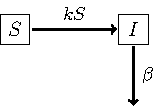
\includegraphics{series_files/figure-latex/quarantine-1.pdf}

Which gives us the following system of equations:
\begin{equation}
\begin{split}\label{eq:flu-quarantine}
\frac{dS}{dt} &= -kSI \\
\frac{dI}{dt} &= kSI - \beta I
\end{split}
\end{equation}

To find the equilibrium solutions we want to find values of \(S\) and \(I\) where the rates \(\displaystyle \frac{dS}{dt}\) and \(\displaystyle \frac{dI}{dt}\) are \emph{both} zero. This can be done by algebraically solving the system of equations:

\begin{align*}
0 &= -kSI \\
0 &= kSI - \beta I
\end{align*}

Let's examine the first equation (\(0 = -kSI\)), which we can see is consistent when either \(S=0\) and \(I=0\). These give us two options, which we then use in the second equation (\(0 = kSI - \beta I\)). When \(S=0\), then \(0 = k\cdot 0 \cdot I - \beta I \rightarrow 0 = -\beta I\), which is consistent when \(I=0\). So \((S_{*},I_{*}) = (0,0)\) is one equilibrium solution. (In fact, if \(I=0\), then any value of \(S\) would be an equilibrium solution. Can you explain why?)

This is an interesting example. We call the equations \(S=0\) and \(I=0\) when \(\displaystyle \frac{dS}{dt}=0\) as \emph{nullclines} for \(S\). In a similar manner, the equations in \(S\) and \(I\) when \(\displaystyle \frac{dI}{dt}=0\) are called \emph{nullclines} for \(I\). Let's try to determine formulas for these equations:

\begin{align*}
0 &= kSI-\beta I \\
0 &= I\cdot (kS - \beta )
\end{align*}

Because the last equation is factored as a product, nullclines for \(I\) are either \(I=0\) or \(\displaystyle S = \frac{\beta}{k}\).

Nullclines are not equilibrium solutions by themselves - it is the \emph{intersection} of two different nullclines that determine equilibrium solutions. Figure \ref{fig:quarantine-nullclines} shows the nullclines in the \(S-I\) plane (since we have two equations), with \(S\) on the horizontal axis and \(I\) on the vertical axis.

\begin{figure}
\centering
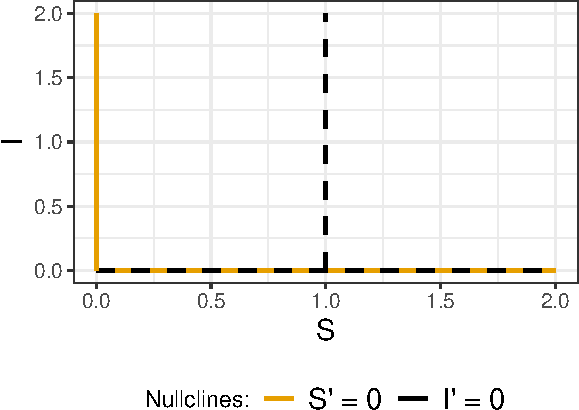
\includegraphics{series_files/figure-latex/quarantine-nullclines-1.pdf}
\caption{\label{fig:quarantine-nullclines}Nullclines for Equation \eqref{eq:flu-quarantine}. To generate the plot we assumed \(\beta=1\) and \(k=1\)}
\end{figure}

\begin{verbatim}
## <ggproto object: Class ScaleDiscrete, Scale, gg>
##     aesthetics: colour
##     axis_order: function
##     break_info: function
##     break_positions: function
##     breaks: S' = 0 I' = 0
##     call: call
##     clone: function
##     dimension: function
##     drop: TRUE
##     expand: waiver
##     get_breaks: function
##     get_breaks_minor: function
##     get_labels: function
##     get_limits: function
##     guide: legend
##     is_discrete: function
##     is_empty: function
##     labels: waiver
##     limits: NULL
##     make_sec_title: function
##     make_title: function
##     map: function
##     map_df: function
##     n.breaks.cache: NULL
##     na.translate: TRUE
##     na.value: grey50
##     name: Nullclines
##     palette: function
##     palette.cache: NULL
##     position: left
##     range: <ggproto object: Class RangeDiscrete, Range, gg>
##         range: NULL
##         reset: function
##         train: function
##         super:  <ggproto object: Class RangeDiscrete, Range, gg>
##     rescale: function
##     reset: function
##     scale_name: hue
##     train: function
##     train_df: function
##     transform: function
##     transform_df: function
##     super:  <ggproto object: Class ScaleDiscrete, Scale, gg>
\end{verbatim}

A key thing to note is that where two different nullclines cross is an \emph{equilibrium solution} to the system of equations. This means that \textbf{both} \(\displaystyle \frac{dS}{dt}\) and \(\displaystyle \frac{dI}{dt}\) are zero at this point. Examining Figure \ref{fig:quarantine-nullclines}, there are three possibilities:

\begin{enumerate}
\def\labelenumi{\arabic{enumi}.}
\tightlist
\item
  At \(S=0\) and \(I=0\) (otherwise known as the origin). This equilibrium solution makes biological sense: if there is nobody susceptible or infected (everyone is perfectly healthy - yay!) there are no flu cases.
\item
  Building on the last equilibrium solution, the entire horizontal axis is an equilibrium solution because the nullclines for \(S\) and \(I\) are the (\(I=0\)). There is a practical interpretation of this nullcline - whenever \(I=0\), meaning there are no infected people around, the solution is at an equilibrium.
\item
  There is also a third possibility where the vertical line at \(S=1\) crosses the horizontal axis (\(S=1\), \(I=0\)), but that also falls under the second equilibrium solution.
\end{enumerate}

Now that we have identified our nullclines and equilibrium solutions, we will add additional context with the \emph{flow} of the solution.

\hypertarget{adding-context-to-our-phase-plane-slope-fields}{%
\subsection{Adding context to our phase plane: slope fields}\label{adding-context-to-our-phase-plane-slope-fields}}

Let's go back to the idea of a phase plane, but this time we are going to add more context to our nullcline graph by evaluating different values of \(S\) and \(I\) into our system of equations and plot the \emph{slope field}.

First let's evaluate the derivatives \(\displaystyle \frac{dS}{dt}\) and \(\displaystyle \frac{dI}{dt}\) in Equation \eqref{eq:flu-quarantine} for different values of \(S\) and \(I\):

\begin{table}

\caption{\label{tab:unnamed-chunk-96}Values of $\frac{dS}{dt}$ and $\frac{dI}{dt}$ for the flu with quarantine model.}
\centering
\begin{tabular}[t]{r|r|r|r}
\hline
S & I & dS\_dt & dI\_dt\\
\hline
0.0000000 & 0.0000000 & 0.0000000 & 0.0000000\\
\hline
0.4444444 & 0.4444444 & -0.1975309 & -0.2469136\\
\hline
0.8888889 & 0.8888889 & -0.7901235 & -0.0987654\\
\hline
1.3333333 & 1.3333333 & -1.7777778 & 0.4444444\\
\hline
1.7777778 & 1.7777778 & -3.1604938 & 1.3827160\\
\hline
2.2222222 & 2.2222222 & -4.9382716 & 2.7160494\\
\hline
2.6666667 & 2.6666667 & -7.1111111 & 4.4444444\\
\hline
3.1111111 & 3.1111111 & -9.6790123 & 6.5679012\\
\hline
3.5555556 & 3.5555556 & -12.6419753 & 9.0864198\\
\hline
4.0000000 & 4.0000000 & -16.0000000 & 12.0000000\\
\hline
\end{tabular}
\end{table}

Notice how the different values of \(\displaystyle \frac{dS}{dt}\) and \(\displaystyle \frac{dI}{dt}\) at each of the \(S\) and \(I\) values. We can plot each of the coordinate pairs of \(\displaystyle \left( \frac{dS}{dt}, \frac{dI}{dt} \right)\) with a vector in the \((S,I)\) plane. We associate \(\displaystyle \frac{dS}{dt}\) with left-right motion, so positive \(\displaystyle \frac{dS}{dt}\) means pointing to the right. Likewise, we associate \(\displaystyle \frac{dI}{dt}\) with up-down motion, so positive \(\displaystyle \frac{dI}{dt}\) means the vector points up. At the point \((S,I)=(1,1)\), we have an arrow that points directly to the west because and \(\displaystyle \frac{dI}{dt} < 0\) and \(\displaystyle \frac{dI}{dt} =0\). If we sequentially sample points in the \((S,I)\) plane we get a vector field plot, superimposed with the nullclines:

\begin{figure}
\centering
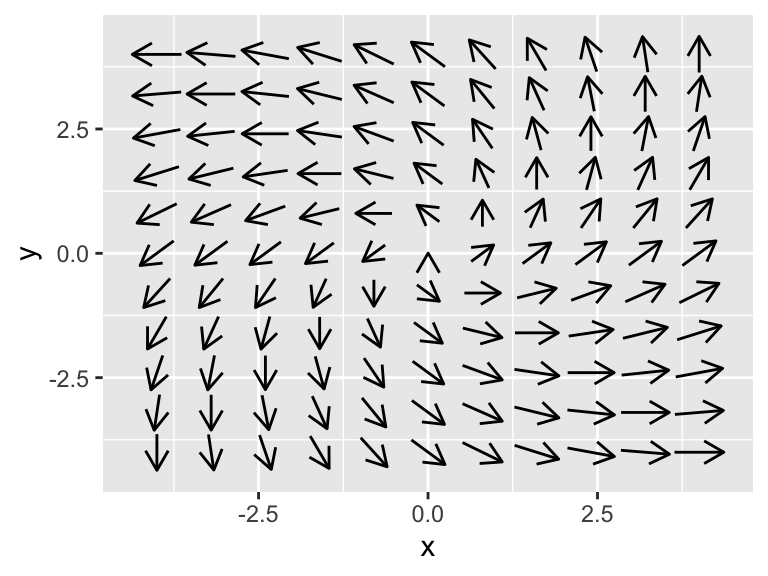
\includegraphics{series_files/figure-latex/unnamed-chunk-97-1.pdf}
\caption{\label{fig:unnamed-chunk-97}Phaseplane for Equation \eqref{eq:flu-quarantine}. To generate the plot we assumed \(\beta=1\) and \(k=1\)}
\end{figure}

\hypertarget{motion-around-the-nullclines}{%
\subsection{Motion around the nullclines}\label{motion-around-the-nullclines}}

We can also extend the motion around the nullclines to investigate the stability. With a one dimensional differential equation we used a number line to quantify values where the solution is increasing / decreasing. The problem with several differential equations is that the notion of ``increasing'' or ``decreasing''" becomes difficult to understand - as there is an additional degree of freedom! Simply put, in a plane you can move left/right \emph{or} up/down. The benefit for having nullclines is that they \textbf{isolate} the motion in one direction.

In general for a two dimensional system:
- When a horizontal axis variable has a nullcline, the only allowed motion is up/down.
- When a vertical axis variable has a nullcline, the only motion is up/down.

Applying this knowledge to Equation \eqref{eq:flu-quarantine}, if we choose points where \(I'=0\) then we know that the only motion is to the left and the right because \(S\) can still change along that curve. If we choose points where \(S'=0\) then we know that the only motion is to the up/down because \(I\) can still change along that curve (Figure \ref{fig:nullclines-quarantine-explained}).

\begin{figure}
\centering
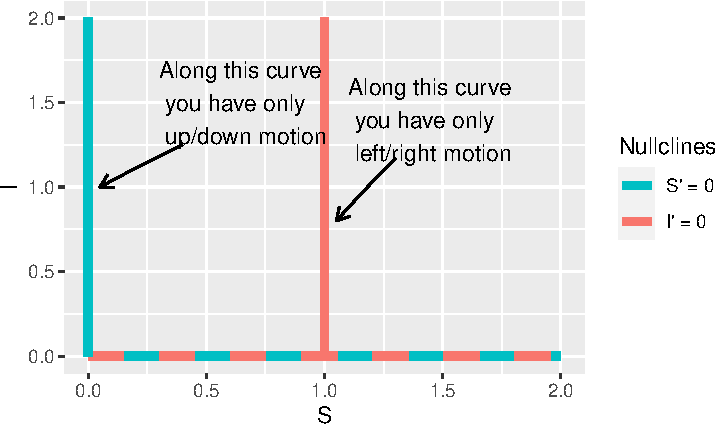
\includegraphics{series_files/figure-latex/nullclines-quarantine-explained-1.pdf}
\caption{\label{fig:nullclines-quarantine-explained}Nullclines for Equation \eqref{eq:flu-quarantine} with context on the direction of the motion.}
\end{figure}

\hypertarget{determining-stability}{%
\section{Determining stability}\label{determining-stability}}

The picture of the phase plane with the nullcline qualitatively tells us about the stability of an equilibrium point. Once of the equilibrium solutions is at the origin \((S,I)=(0,0)\). As before we want to investigate if the equilibrium solution is stable or unstable.

Figure \ref{fig:zoom-quarantine-plane} zooms in the phaseplane at the equilibrium solution at \(S=0\), \(I=0\):

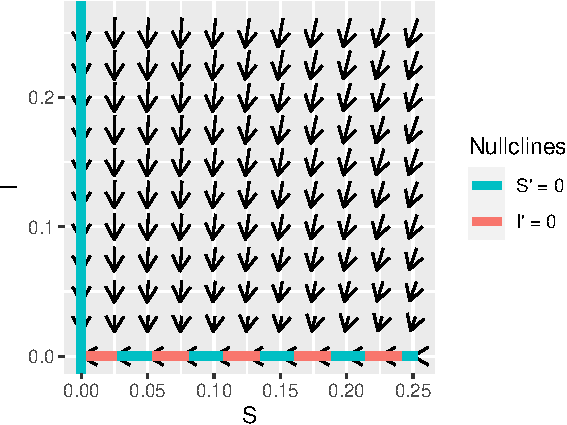
\includegraphics{series_files/figure-latex/zoom-quarantine-plane-1.pdf}

As you can see the arrows appear to be pointing into and towards the equilibrium solution. So we would classify this equilbrium solution as \emph{stable}.

\hypertarget{generating-a-phase-plane-in-r}{%
\section{\texorpdfstring{Generating a phase plane in \texttt{R}}{Generating a phase plane in R}}\label{generating-a-phase-plane-in-r}}

Let's take what we learned from the case study of the flu model with quarantine to qualitatively analyze a system of differential equations:

\begin{itemize}
\tightlist
\item
  We determine nullclines by setting the derivatives equal to zero.
\item
  Equilibrium solutions occur where nullclines for the two different equations intersect.
\item
  The arrows in the phase plane help us characterize the stability of the equilibrium solution.
\end{itemize}

To determine the phaseplane diagram \texttt{demodelr} package has some basic functionality to generate a phase plane. Consider the following system of differential equations (Equation \eqref{eq:phase-example}):

\begin{equation}
\begin{split}\label{eq:phase-example}
\frac{dx}{dt} &= x-y \\
\frac{dy}{dt} &= -x+y
\end{split}
\end{equation}

In order to generate a phaseplane diagram for Equation \eqref{eq:phase-example} we need to define functions for \(x'\) and \(y'\), which I will annotate as \(dx\) and \(dy\) respectively. We are going to collect these equations in one vector called \texttt{system\_eq}, using the tilde (\textasciitilde) as a replacement for the equals sign:

\begin{Shaded}
\begin{Highlighting}[]
\NormalTok{system\_eq }\OtherTok{\textless{}{-}} \FunctionTok{c}\NormalTok{(dx }\SpecialCharTok{\textasciitilde{}}\NormalTok{ x}\SpecialCharTok{{-}}\NormalTok{y,}
\NormalTok{               dy }\SpecialCharTok{\textasciitilde{}}\NormalTok{ x}\SpecialCharTok{+}\NormalTok{y)}
\end{Highlighting}
\end{Shaded}

Then what we do is apply the command \texttt{phaseplane}, which will generate a vector field over a domain:

\begin{Shaded}
\begin{Highlighting}[]
\FunctionTok{phaseplane}\NormalTok{(system\_eq,}\StringTok{\textquotesingle{}x\textquotesingle{}}\NormalTok{,}\StringTok{\textquotesingle{}y\textquotesingle{}}\NormalTok{)  }\CommentTok{\# The values in quotes are the labels for the axes and to identify the variables {-} they are needed!}
\end{Highlighting}
\end{Shaded}

\begin{figure}
\centering
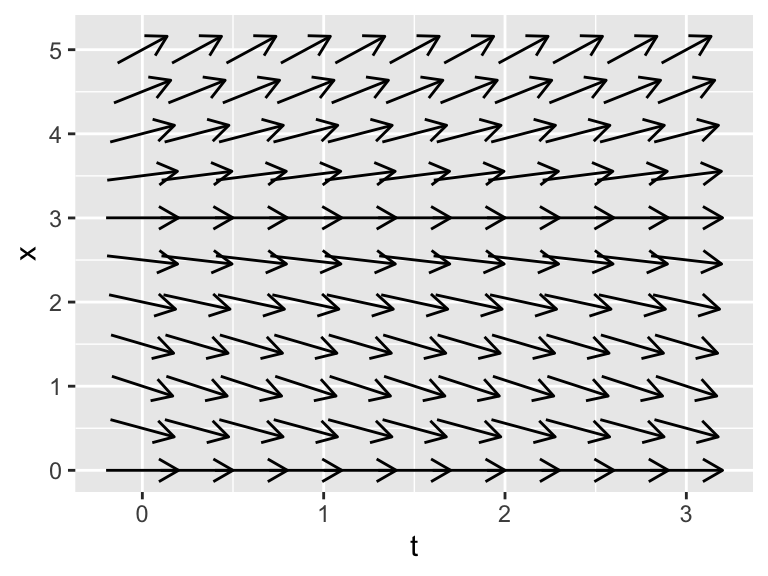
\includegraphics{series_files/figure-latex/unnamed-chunk-99-1.pdf}
\caption{\label{fig:unnamed-chunk-99}Phaseplane diagram for Equation \eqref{eq:phase-example}}
\end{figure}

The command \texttt{phaseplane} has an option called \texttt{eq\_soln} that will if there are any equilibrium solutions to be found and report them to the console. For example try running \texttt{phaseplane(system\_eq,\textquotesingle{}x\textquotesingle{},\textquotesingle{}y\textquotesingle{},eq\_soln=TRUE)} and see what gets output to console. While this option lists equilibrium solutions, you should confirm them with the differential equation through direct solving.

\hypertarget{generating-a-phase-line-in-r}{%
\subsection{Generating a phase line in R:}\label{generating-a-phase-line-in-r}}

From Section \ref{phase-05} we discussed how to construct phaselines by hand. It turns out that the command \texttt{phaseplane} can also plot phase lines. Let's take a look at an example first and then discuss how that it works.

\begin{example}
\protect\hypertarget{exm:unnamed-chunk-100}{}{\label{exm:unnamed-chunk-100} }A colony of bacteria growing in a nutrient-rich medium deplete the nutrient as they grow. As a result, the nutrient concentration \(x(t)\) is steadily decreasing. Determine the phaseline for the following differential equation:

\begin{equation}\label{eq:bacteria-colony}
\frac{dx}{dt} = - 0.7 \cdot \frac{x \cdot (3- x)}{1 + x}
\end{equation}
\end{example}

The R code to generate this phaseline is the following:

\begin{Shaded}
\begin{Highlighting}[]
\CommentTok{\# Define the windows where we make the plots}
\NormalTok{t\_window }\OtherTok{\textless{}{-}} \FunctionTok{c}\NormalTok{(}\DecValTok{0}\NormalTok{,}\DecValTok{3}\NormalTok{)}
\NormalTok{x\_window }\OtherTok{\textless{}{-}} \FunctionTok{c}\NormalTok{(}\DecValTok{0}\NormalTok{,}\DecValTok{5}\NormalTok{)}

\CommentTok{\# Define the differential equation}
\NormalTok{system\_eq }\OtherTok{\textless{}{-}} \FunctionTok{c}\NormalTok{(dt }\SpecialCharTok{\textasciitilde{}} \DecValTok{1}\NormalTok{,}
\NormalTok{               dx }\SpecialCharTok{\textasciitilde{}} \SpecialCharTok{{-}}\FloatTok{0.7} \SpecialCharTok{*}\NormalTok{ x}\SpecialCharTok{*}\NormalTok{(}\DecValTok{3}\SpecialCharTok{{-}}\NormalTok{x)}\SpecialCharTok{/}\NormalTok{(}\DecValTok{1}\SpecialCharTok{+}\NormalTok{x))}

\FunctionTok{phaseplane}\NormalTok{(system\_eq,}\StringTok{"t"}\NormalTok{,}\StringTok{"x"}\NormalTok{,t\_window,x\_window)}
\end{Highlighting}
\end{Shaded}

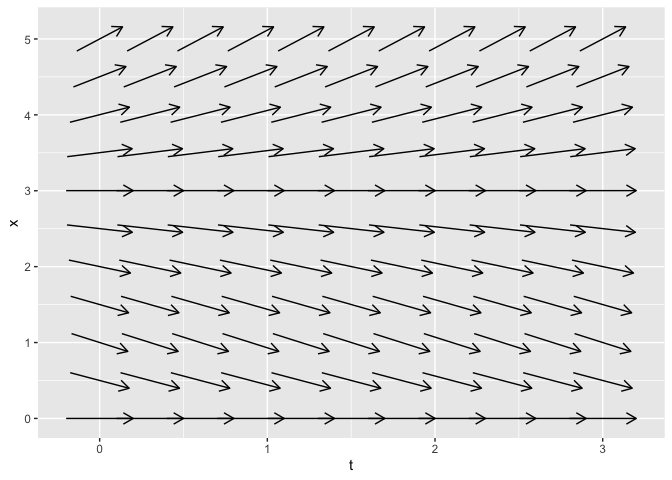
\includegraphics{series_files/figure-latex/unnamed-chunk-101-1.pdf}

Notice how we have the equation \(dt = 1\). What we are doing is re-writing the differential equation with a new variable \(s\) (Equation \eqref{eq:single-phase}):

\begin{equation}
\begin{split}\label{eq:single-phase}
\frac{dt}{ds} &= 1 \\
\frac{dx}{ds} &= - 0.7 \cdot \frac{x \cdot (3- x)}{1 + x}
\end{split}
\end{equation}

The differential equation \(\displaystyle \frac{dt}{ds} = 1\) has solution \(s=t\), so in essence is the same as Equation \eqref{eq:bacteria-colony} (perhaps a little more complicated). However re-writing this system was a quick and handy workaround to re-use code.

\hypertarget{exercises-5}{%
\section{Exercises}\label{exercises-5}}

\begin{exercise}
\protect\hypertarget{exr:unnamed-chunk-102}{}{\label{exr:unnamed-chunk-102} }Determine equilibrium solutions for Equation \eqref{eq:phase-example}.
\end{exercise}

~

\begin{exercise}
\protect\hypertarget{exr:unnamed-chunk-103}{}{\label{exr:unnamed-chunk-103} }This problem considers the following system of differential equations:
\begin{align*} 
\frac{dx}{dt} &= y \\ 
\frac{dy}{dt} &= -x 
\end{align*}

\begin{enumerate}[label=\alph*.]
\item Determine the equations of the nullclines and equilibrium point of this system of differential equations.
\item Modify the function \texttt{phaseplane} to generate a phaseplane of this system.
\item For each point along a nullcline, determine the resulting motion (up-down or left-right).
\item Based on the work you generated, determine if the equilibrium solution is \emph{stable} or \emph{unstable}.
\item Verify that the functions $x(t) = \sin(t)$ and $y=\cos(t)$ is one solution to this system of differential equations.
\end{enumerate}
\end{exercise}

~

\begin{exercise}
\protect\hypertarget{exr:unnamed-chunk-104}{}{\label{exr:unnamed-chunk-104} }Considers the following system of differential equations:

\begin{equation} 
\begin{split}
\frac{dx}{dt} &= y \\ 
\frac{dy}{dt} &= 3x^{2}-1 
\end{split}
\end{equation}

\begin{enumerate}[label=\alph*.]
 \item Determine the equations of the nullclines and equilibrium solutions for this system of differential equations.
\item For each point along a nullcline, determine the resulting motion (up-down or left-right).
\item Modify the function \texttt{phaseplane} to generate a phaseplane of this system.
\item  Make a hypothesis to classify if the equilibrium point is \emph{stable} or \emph{unstable}.
\end{enumerate} 
\end{exercise}

~

\begin{exercise}
\protect\hypertarget{exr:unnamed-chunk-105}{}{\label{exr:unnamed-chunk-105} }A plant grows propritional to its current length \(L\). Assume this proportionality constant is \(\mu\), whose rate also decreases proportional to its current value. The system of equations that models this plant growth is the following:
\begin{equation}
\begin{split}
\frac{dL}{dt} &= \mu L \\ 
\frac{d\mu}{dt}  &= -0.1 \mu \\
\end{split}
\end{equation}

\begin{enumerate}[label=\alph*.]
 \item Explain why $L=0$ and $\mu=0$ is the only equilibrium solution to this differential equation.
\item Modify the function \texttt{phaseplane} to generate a phaseplane of this system.
\item Is the origin a stable equilibrium solution?
\end{enumerate}
\end{exercise}

~

\begin{exercise}
\protect\hypertarget{exr:unnamed-chunk-106}{}{\label{exr:unnamed-chunk-106} }Red blood cells are formed from stem cells in the bone marrow. The red blood cell density \(r\) satisfies an equation of the form

\begin{equation}
\frac{dr}{dt} = \frac{0.2r}{1+r^{2}} -  0.1 r,
\end{equation}

\begin{enumerate}[label=\alph*.]
 \item What are the equilibrium solutions for this differential equation?
\item Modify the function \texttt{phaseplane} to generate a phaseline for this differential euqation for $0 \leq t \leq 5$ and $0 \leq r \leq 5$.
\item Based on the phaseline, are the equilibrium solutions stable or unstable?
\end{enumerate}
\end{exercise}

~

\begin{exercise}
\protect\hypertarget{exr:unnamed-chunk-107}{}{\label{exr:unnamed-chunk-107} }Organisms that live in a saline environment biochemically maintain the amount of salt in their blood stream. An equation that represents the level of \(S\) in the blood is the following:

\[ \frac{dS}{dt} = 1 + 0.3 \cdot (3 - S) \]

\begin{enumerate}[label=\alph*.]
\item What are the equilibrium solutions for this differential equation?
\item Modify the function \texttt{phaseplane} to generate a phaseline for this differential euqation for $0 \leq t \leq 10$ and $0 \leq S \leq 10$.
\item Based on the phaseline, are the equilibrium solutions stable or unstable?
\end{enumerate}
\end{exercise}

~

\begin{exercise}
\protect\hypertarget{exr:unnamed-chunk-108}{}{\label{exr:unnamed-chunk-108} }The core body temperature (\(T\)) of a mammal is coupled to the heat production (scaled by heat capacity \(Q\)) with the following system of differential equations:
\begin{equation}
\begin{split}
\frac{dT}{dt} &= Q + 0.5 \cdot (20-T) \\ 
\frac{dQ}{dt} &= 0.1 \cdot (38-T),
\end{split}
\end{equation}

\begin{enumerate}[label=\alph*.]
 \item Determine the equations of the nullclines and equilibrium point of this system of differential equations.
\item For each point along a nullcline, determine the resulting motion (up-down or left-right).
\item  Make a hypothesis to classify if the equilibrium point is \emph{stable} or \emph{unstable}.
\end{enumerate}
\end{exercise}

~

\begin{exercise}
\protect\hypertarget{exr:unnamed-chunk-109}{}{\label{exr:unnamed-chunk-109} }Consider the following system of differential equations for the lynx-hare model:
\begin{align}
\frac{dH}{dt} &= r H - b HL \\
\frac{dL}{dt} &=ebHL -dL
\end{align}

\begin{enumerate}[label=\alph*.]
\item Determine the steady states of this system of differential equations.
\item Determine equations for the nullclines, expressed as $L$ as a function of $H$.  There should be two nullclnes for each rate. 
\end{enumerate}
\end{exercise}

~

\begin{figure}
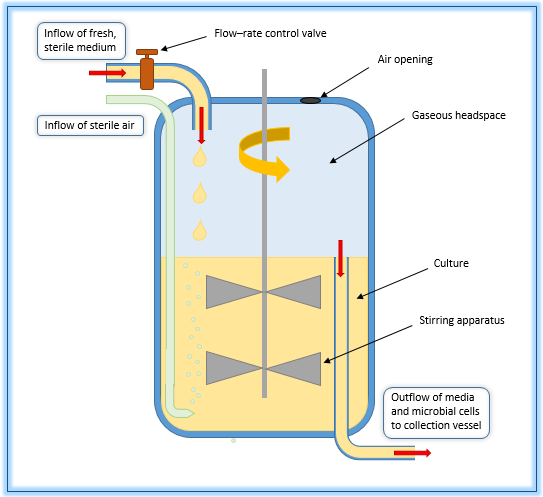
\includegraphics[width=4in]{figures/06-coupledSystems/Chemostat_Vessel_Diagram} \caption{\label{fig:chemostat}An example of a chemostat.}\label{fig:unnamed-chunk-110}
\end{figure}

\begin{exercise}
\protect\hypertarget{exr:unnamed-chunk-111}{}{\label{exr:unnamed-chunk-111} }A chemostat is a tank used to study microbes and ecology, where microbes grow under controlled conditions. Think of this like a large tank with nutrient-rich water being continuously cycled through, as shown in the following Figure \ref{fig:chemostat} (Source: \href{https://en.wikipedia.org/wiki/Chemostat}{Wikipedia}). Equations that describe the microbial biomass \(W\) and the nutrient concentration \(C\) (in the culture) are the following:

\begin{align}
\frac{dW}{dt} &= \mu W - F \frac{W}{V} \\
\frac{dC}{dt} &= D \cdot (C_{R}-C) - S \mu \frac{W}{V},
\end{align}

where we have the following parameters: \(\mu\) is the per capita reproduction rate, \(F\) is the flow rate, \(V\) is the volume of the culture solution, \(D\) is the dilution rate, \(C_{R}\) is the concentration of nutrients entering the culture, and \(S\) is a stoichiometric conversion of nutrients to biomass.

\begin{enumerate}[label=\alph*.]
 \item Write the equations of the nullclines for this differential equation.
 \item Determine the equilibrium solutions for this system of differential equations.
 \item Generate a phaseplane for this differential equation with the values $\mu=1$, $D=1$, $C_{R}=2$ and $S=1$ and $V=1$.
 \item Classify the stability of the equilbrium solutions.
 \end{enumerate}
\end{exercise}

~

\begin{figure}
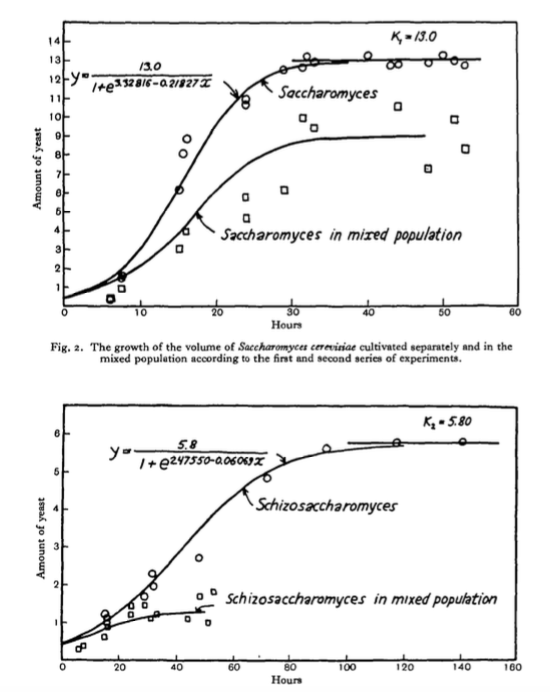
\includegraphics[width=4in]{figures/06-coupledSystems/gause-results} \caption{\label{fig:gause}Population results from two yeast species growing in competition. From Gause (1932)}\label{fig:unnamed-chunk-112}
\end{figure}

\begin{exercise}
\protect\hypertarget{exr:unnamed-chunk-113}{}{\label{exr:unnamed-chunk-113} } A classical paper \emph{Experimental Studies on the Struggle for Existence: I. Mixed Population of Two Species of Yeast} by Gause (1932) examined two different species of yeast growing in competition with each other. The differential equations given for two species in competition are:

\begin{align*}
\frac{dy_{1}}{dt} &= -b_{1} y_{1} \frac{(K_{1}-(y_{1}+\alpha y_{2}) )}{K_{1}} \\
\frac{dy_{2}}{dt} &= -b_{2} y_{2} \frac{(K_{2}-(y_{2}+\beta y_{1}) )}{K_{2}}, \\
\end{align*}

where \(y_{1}\) and \(y_{2}\) are the two species of yeast with the parameters \(b_{1}, \; b_{2}, \; K_{1}, \; K_{2}, \; \alpha, \; \beta\) describing the characteristics of the yeast species.

\begin{enumerate}[label=\alph*.]
\item Determine the equilibrium solutions for this differential equation.  Express your answer in terms of the parameters $b_{1}, \; b_{2}, \; K_{1}, \; K_{2}, \; \alpha, \; \beta$.
\item Gause computed the following values of the parameters: $b_{1}=0.21827, \; b_{2}=0.06069, \; K_{1}=13.0, \; K_{2}=5.8, \; \alpha=3.15, \; \beta=0.439$.  Using these values, what would be the predicted values for the equilibrium solutions?
\item Use the function \texttt{systems} to solve this system of differential equations numerically.
   
   \item Figure \ref{fig:gause} is from Gause (1932) and shows the experimental population values ``in mixed population''.  Use the graph to estimate the equilibrium solutions for both species. How close (or how far from) the equilibrium solutions are Gause's results to your computed equilibrium solutions?

\end{enumerate}
\end{exercise}

\hypertarget{exact-solns-07}{%
\chapter{Exact Solutions to Differential Equations}\label{exact-solns-07}}

We have already discussed some tools that can analyze differential equations numerically (Section \ref{euler-04}) and qualitatively (Sections \ref{phase-05} and \ref{coupled-06}). The phase plane allowed us to evaluate equilibrium solutions and their stability. Beyond this graphical approach, it is also helpful to know the exact solution to an equation. In this section we will study a few techniques to find exact solutions to differential equation. We will apply some of the tools you may have learned from calculus.

\hypertarget{separable-differential-equations}{%
\section{Separable Differential Equations}\label{separable-differential-equations}}

One technique to solve differential equations is the method of \emph{separation of variables}. Let's look at an example:

What is the general solution to \(\displaystyle \frac{dy}{dx} = yx^{2}\)? To solve this expression we collect the variables involving \(x\) and one side of the equation, and the variables involving \(y\) on the other:

\begin{equation*}
\frac{1}{y} dy = x^{2} dx.
\end{equation*}

Now the next step is to determine the antiderivative of both sides of expression:

\begin{equation*}
\begin{split}
\int  \frac{1}{y} dy = \ln(y) + C. \\
\int x^{2} dx  = \frac{1}{3} x^{3} + C.
\end{split}
\end{equation*}

Finally since both sides are equal we can solve for the dependent variable \(y\). One thing to note: usually for antiderivatives we always include a \(+C\). For solving differential equations it is okay just to keep only one \(+C\), which usually is best on the side of the independent variable:

\begin{equation*}
\ln(y) =\frac{1}{3} x^{3} + C \rightarrow e^{\ln(y)} = e^{\frac{1}{3} x^{3} + C} \rightarrow y = Ce^{\frac{1}{3} x^{3}}.
\end{equation*}

We are in business! So here is a general technique approach to solving a differential equation via separation of variables:

\begin{enumerate}
\def\labelenumi{\arabic{enumi}.}
\tightlist
\item
  \textbf{Separate} the variables on one side of the equation.
\item
  \textbf{Integrate} both sides individually.
\item
  \textbf{Solve} for the dependent variable.
\end{enumerate}

If we solve this equation using separation of variables we havUsing your work above as a guide, solve this differential equation to determine a solution \(y(x)\).

\hypertarget{integrating-factors}{%
\section{Integrating factors}\label{integrating-factors}}

One model that we have looked at is the the \(SI\) model where the spread of the disease is proportional to the number infected:

\begin{equation*}
\frac{dI}{dt} = .03(1000-I) = 30  - .03I
\end{equation*}

While this differential equation can be solved via separation of variables, let's try a different approach as an illustration of another useful technique. First let's write the terms involving \(I\) on one side of the equation:

\begin{equation*}
\frac{dI}{dt} + .03I = 30.
\end{equation*}

What we are going to do is multiply both sides of this equation by \(e^{.03t}\) (I'll explain more about that later):

\begin{equation*}
\frac{dI}{dt} \cdot e^{.03t} + .03I \cdot e^{.03t} = 30  \cdot e^{.03t}
\end{equation*}

Hmmm - this seems like we are making our equation harder to solve, doesn't it? However the left hand side is actually the derivative of the expression \(I \cdot e^{kt}\)! Let's take a look:

\begin{equation*}
\frac{d}{dt} \left( I \cdot e^{.03t} \right) = \frac{dI}{dt} \cdot e^{.03t} + I \cdot .03 e^{.03t}
\end{equation*}

This derivative is courtesy of the product rule from calculus. Ok, so what does this do to the differential equation? Well, by re-writing the differential equation as a derivative and integrating:

\begin{equation}
\begin{split}
\frac{d}{dt} \left( I \cdot e^{.03t} \right) &= 30 \cdot e^{.03t} \rightarrow \\
\int \frac{d}{dt} \left( I \cdot e^{.03t} \right) \; dt &= \int 30 \cdot e^{.03t} \; dt \rightarrow \\
I \cdot e^{.03t} &= 30 \cdot e^{.03t} + C
\end{split}
\end{equation}

Notice how by writing the left hand side in terms of the product rule and integrating we could find the solution. We added the \(+C\) to the right hand side. All that is left to do is to solve in terms of \(I(t)\) by dividing by \(e^{kt}\). We will label this solution \(I_{1}(t)\):

\begin{equation}
I_{1}(t) = 1000 + Ce^{-.03t}  \label{eq:i1}
\end{equation}

Cool! The function \(e^{.03t}\) is called an \emph{integrating factor}. To see what is meant by that, let's try one more example.

In this case, we are going to assume that the rate of infection is time dependent, or \(k(t) = .03t\). How this would work in practice is that initially (at \(t=0\)) there is no infection, but the infection rate increases as time goes on.

Our differential equation in this case is:

\begin{equation*}
\frac{dI}{dt} + .03 t \cdot I = 30 t.
\end{equation*}

So if we want to write the left hand side as a product, what we will do is multiply the \emph{entire} differential equation by \(\displaystyle e^{\int .03t \; dt} = e^{ 0.015 t^{2}}\) This term is called the \emph{integrating factor}:

\begin{equation*}
\frac{dI}{dt} \cdot e^{ 0.015 t^{2}} + .03 t \cdot I \cdot e^{0.015 t^{2}} = 30 t \cdot e^{0.015 t^{2}}
\end{equation*}

First we rewrite the left hand side using the product rule:
\begin{equation*}
\frac{dI}{dt} \cdot e^{ 0.015 t^{2}} + .03 t \cdot I \cdot e^{0.015 t^{2}} = \frac{d}{dt} \left( I \cdot e^{0.015  t^{2}} \right). 
\end{equation*}

Now we can integrate this equation by:

\begin{equation}
\begin{split}
\frac{d}{dt} \left( I \cdot e^{0.015 t^{2}} \right) &= 30 t \cdot e^{0.015 t^{2}}  \rightarrow \\
\int \frac{d}{dt} \left( I \cdot e^{0.015  t^{2}} \right) \; dt &= \int 30t \cdot e^{0.015 t^{2}}  \; dt \rightarrow \\
I \cdot e^{0.015 t^{2}} &= N \cdot e^{0.015 t^{2}} + C
\end{split}
\end{equation}

All right! So the last step is to write the equation in terms of \(I(t)\), which we will label \(I_{2}(t)\):

\begin{equation}
I_{2}(t) =  1000 + C e^{-0.015 t^{2}}  \label{eq:i2}
\end{equation}

Figure \ref{fig:if-compare} compares solutions when \(I(0)=10\).

\begin{figure}
\centering
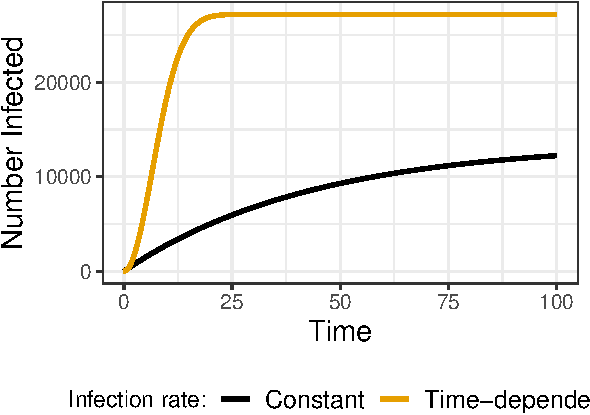
\includegraphics{series_files/figure-latex/if-compare-1.pdf}
\caption{\label{fig:if-compare}Comparison of two integrating factor solutions, Equation \eqref{eq:i1} in red and Equation \eqref{eq:i2} in blue.}
\end{figure}

Ok, let's summarize this integrating factor approach for differential equations that can be written in the form \[\frac{dy}{dt} + f(t) \cdot y = g(t)\]

\begin{enumerate}
\def\labelenumi{\arabic{enumi}.}
\tightlist
\item
  Calculate the \emph{integrating factor} \(\displaystyle e^{\int f(t) \; dt}\). Hopefully the integral \(\displaystyle \int f(t) \; dt\) is easy to compute!
\item
  Next multiply the integrating factor across your equation to rewrite the differential equation as \(\displaystyle \frac{d}{dt} \left( y \cdot e^{\int f(t) \; dt} \right) = g(t) \cdot e^{\int f(t) \; dt}\).
\item
  Then compute the integral \(\displaystyle H(t) = \int g(t) \cdot e^{\int f(t) \; dt} \; dt\). This looks intimidating - but hopefully is manageable to compute! Don't forget the \(+C\)!
\item
  Then solve for \(y(t)\): \(\displaystyle y(t) = H(t) \cdot e^{-\int f(t) \; dt} + C e^{-\int f(t) \; dt}\).
\end{enumerate}

This technique is a handy way to work with equations that aren't easily separable.

\hypertarget{guess-and-check}{%
\section{Guess and Check}\label{guess-and-check}}

A final approach is called the guess and check method. Say for example we have the following equation that describes the rate of change above: The first approach if a function is a solution to a differential equation is the guess and check method, or by direct substitution.

\[ \frac{dS}{dt} = 0.7 S \]

We know that we can apply separation of variables, but instead let's try to see if the function \(\tilde{S}(t) = 5 e^{0.7t}\) is a solution in order to do that, we need to differentiate \(\tilde{S}(t)\), which using our knowledge of calculus is \(0.7 \cdot 5 e^{-0.7t}\). If we note that \(\displaystyle \frac{d\tilde{S}}{dt} = 0.7 \tilde{S} = 0.7 e^{0.7t}\) than the function \(\tilde{S}\) does solve the differential equation.

Super cool! Let's try an example:

\begin{example}
\protect\hypertarget{exm:unnamed-chunk-114}{}{\label{exm:unnamed-chunk-114} }Verify the following functions are solutions to the differential equation \(\displaystyle \frac{dS}{dt} = 0.7 S\):

\begin{itemize}
\tightlist
\item
  \(\tilde{R}(t) = 10e^{0.7t}\)
\item
  \(\tilde{P}(t) = e^{0.7t}\)
\item
  \(\tilde{Q}(t) = 5e^{0.7t}\)
\item
  \(\tilde{F}(t)=3\)
\item
  \(\tilde{G}(t)=0\)
\end{itemize}
\end{example}

\begin{remark}
\iffalse{} {Remark. } \fi{}Let's apply direct differentiation to each of these functions:

\begin{itemize}
\tightlist
\item
  \(\tilde{R}(t) = 10e^{0.7t} \rightarrow \tilde{R}'(t) = 7e^{0.7t}\)
\item
  \(\tilde{P}(t) = e^{0.7t} \rightarrow \tilde{P}'(t) = e^{0.7t}\)
\item
  \(\tilde{Q}(t) = 5e^{0.7t} \rightarrow \tilde{Q}'(t) = 3.5e^{0.7t}\)
\item
  \(\tilde{F}(t)=3 \rightarrow \tilde{F}'(t) = 0\)
\item
  \(\tilde{G}(t)=0 \rightarrow \tilde{G}'(t) = 0\)
\end{itemize}

Now we will compare each of these solutions to the right hand side:

\begin{itemize}
\tightlist
\item
  \(0.7\tilde{R}(t) = 0.7 \cdot 10e^{0.7t} \rightarrow 7e^{0.7t}\)
\item
  \(0.7\tilde{P}(t) = 0.7 e^{0.7t}\)
\item
  \(0.7\tilde{Q}(t) = 0.7 \cdot 5e^{0.7t} \rightarrow = 3.5e^{0.7t}\)
\item
  \(0.7 \tilde{F}(t)=0.7 \cdot 3 \rightarrow 2.1\)
\item
  \(0.7 \tilde{G}(t)=0.7 \cdot 0 \rightarrow 0\)
\end{itemize}

Notice how the right hand sides of each equation equals the left hand sides. When that is the case, our candidate functions are indeed solutions to the differential equation!
\end{remark}

\hypertarget{superposition-of-solutions}{%
\section{Superposition of solutions}\label{superposition-of-solutions}}

Related to the Guess and Check method is this concept called superposition of solutions. Here how this works: if you have two known solutions to a differential equation, then the sum (or difference) is a solution as well. Let's look at an example:

\begin{example}
\protect\hypertarget{exm:unnamed-chunk-116}{}{\label{exm:unnamed-chunk-116} }Show that \(\tilde{S}(t) = 5e^{0.7t} + e^{0.7t}\) is a solution to the differential equation \(\displaystyle \frac{dS}{dt} = 0.7 S\)
\end{example}

\begin{remark}
\iffalse{} {Remark. } \fi{}By direct differentiation, \(\tilde{S}'(t) = 3.5e^{0.7t} + 0.7e^{0.7t}\). Also we have that \(0.7 \cdot \tilde{S}(t) = 0.7 \cdot (5e^{0.7t} + e^{0.7t}) = 3.5 e^{0.7t} + 0.7 e^{0.7t}\), which equals \(\tilde{S}\).
\end{remark}

What this example illustrates is the principle that if you have two solutions to a differential equation, they can be added together and produce a new solution. This is an example of a \emph{linear combinations} of solutions, and we can state this more formally:

\begin{quote}
If \(x(t)\) and \(y(t)\) are solutions to the differential equation \(z' = f(t,z)\), then \(c(t) = a \cdot x(t) + b \cdot y(t)\) are also solutions, where \(a\) and \(b\) are constants.
\end{quote}

Hopefully you were able to verify that \(\tilde{R}\) and \(\tilde{Q}\) and \(\tilde{G}\) all were solutions to the differential equation, and that \(\tilde{R} + \tilde{Q}\) was a solution as well. The most general solution to this differential equation is \(S(t)=Ce^{0.7t}\), where the initial condition would determine the value of \(C\).

\hypertarget{applying-guess-and-check-more-broadly}{%
\section{Applying guess and check more broadly}\label{applying-guess-and-check-more-broadly}}

As noted earlier, the guess and check method may seem to be trivial - if you have a differential equation, and solution, why verify it? Well, this method helps to introduce a useful solution technique to a differential equation, and one that we can build up through directverification.

We are going to revisit the lynx hare model, but simplified a little bit. Here we are going to assume that lynx and hares both decline at a rate proportional to the population size, but the lynx population increases according to the rate of hare decline:

\begin{align}
\frac{dH}{dt} &= -b H  \\
\frac{dL}{dt} & = b H  - d L
\end{align}

Based on these simplified assumptions a good approach is to assume a solution that is exponential for both \(H\) and \(L\):

\begin{align}
\tilde{H}(t) &= C_{1} e^{\lambda t} \\
\tilde{L}(t) &= C_{2} e^{\lambda t}
\end{align}

The form of this solution has three unknowns: \(C_{1}\), \(C_{2}\), and \(\lambda\). If you have had Linear Algebra, you may recognize that we are assuming the solution is a vector of the form \(\vec{v} = \vec{C} e^{\lambda t}\) . Let's apply Guess and Check to solve these equations. By differentiation, we have the following:

\begin{align}
\frac{d\tilde{H}}{dt} &= \lambda C_{1} e^{\lambda t} \\
\frac{d\tilde{L}}{dt}  &= \lambda C_{2} e^{\lambda t}.
\end{align}

Comparing to our differential equation we can show that

\begin{align}
\lambda C_{1} e^{\lambda t} &= - b C_{1} e^{\lambda t} \rightarrow  (\lambda +\delta) C_{1} e^{\lambda t} = 0\\
 \lambda C_{2} e^{\lambda t} &= b  C_{1} e^{\lambda t} - d C_{2} e^{\lambda t}
\end{align}

Let's rearrange this expression a little bit:

\begin{align}
 (\lambda + b) C_{1} e^{\lambda t} &= 0\\
 (\lambda + d) C_{2} e^{\lambda t} &=b  C_{1} e^{\lambda t}
\end{align}

Notice that for the second equation we can solve for \(C_{1} e^{\lambda t}\), or \(\displaystyle C_{1} e^{\lambda t} = \frac{(\lambda + d)}{b} C_{2} e^{\lambda t}\).

This allows for something neat to happen. We can substitute this expression for \(C_{1} e^{\lambda t}\) into the first equation:

\begin{equation}
 (\lambda + b) \frac{(\lambda + d)}{b} C_{2} e^{\lambda t} = 0
\end{equation}

If we assume that \(b \neq 0\), then we have the following simplified expression:

\begin{equation}
(\lambda +b) (\lambda +d) C_{2} e^{\lambda t}  = 0
\end{equation}

Because the exponential function never equals zero, with this new equation, the only possibility is that \((\lambda + b)(\lambda + d)=0\), or that \(\lambda = -b\) or \(\lambda = -d\).Remember: if expressions multiply to zero, then the only possibility is that at least one of them is zero. This process finds the \emph{eigenvalues} and \emph{eigenvectors} of a system of equations. We will study this later in the course.

We now need to determine values of \(C_{1}\) and \(C_{2}\). We can do this by going back to the equation \((\lambda + d) C_{2} e^{\lambda t} =b C_{1} e^{\lambda t}\), or \((\lambda + d) C_{2} e^{\lambda t} -b C_{1} e^{\lambda t}=0\) rearranged.

Let's analyze this equation for each of the values of \(\lambda\):

\hypertarget{case-lambda--d}{%
\subsection{\texorpdfstring{Case \(\lambda = -d\)}{Case \textbackslash lambda = -d}}\label{case-lambda--d}}

For this situation, we have

\[(-d +d) C_{2} e^{-d t} - b  C_{1} e^{-d t} =0 \rightarrow   -b  C_{1} e^{-d t} =0.\]

The only way for this equation to be consistent and remain zero is if \(C_{1}=0\). We don't have any restrictions on \(C_{2}\), so the general solution will be

\begin{align}
\tilde{H}(t) &=0 \\
\tilde{L}(t) &= C_{2} e^{-d t}.
\end{align}

\hypertarget{case-lambda--d-1}{%
\subsection{\texorpdfstring{Case \(\lambda = -d\)}{Case \textbackslash lambda = -d}}\label{case-lambda--d-1}}

For this situation, we have \((-d +b) C_{2} e^{-d t} - d C_{1} e^{-d t} =0\) which leads to the following equation:
\begin{equation}
\left( (-d +b) C_{2} - d  C_{1} \right) e^{-d t} =0
\end{equation}

The only way for this equation to be consistent and remain zero is if \(\left( (-d +b) C_{2} - d C_{1} \right)=0\), or if \(\displaystyle C_{2} = \left( \frac{d}{-d + b} \right) C_{1}\). In this case, the general solution will be

\begin{align}
\tilde{H}(t) &=  C_{1} e^{-d t} \\
\tilde{L}(t) &= \left( \frac{d}{-d + b} \right) C_{1} e^{-d t},
\end{align}

The parameter \(C_{2}\) can be determined by the initial condition. Notice that we need to have \(d \neq b\) or our solution will be undefined.

Now we can write down a general solution to the system by combining our two solutions together. Here we can you the fact that two solutions can be added together (superposition) to generate a solution.

\begin{align}
H(t) &=  C_{1} e^{-d t} \\
L(t) &= \left( \frac{d}{-d + b} \right) C_{1} e^{-d t} + C_{2} e^{-b t}
\end{align}

This method only works on \emph{linear} differential equations (i.e.~it wouldn't work if there was a term such as \(kHL\) in our dynamics. Later on in the course we will look a more systematic method (i.e eigenvalues) to determine solutions to linear systems of equations.

\newpage

\hypertarget{exercises-6}{%
\section{Exercises}\label{exercises-6}}

\begin{exercise}
\protect\hypertarget{exr:unnamed-chunk-118}{}{\label{exr:unnamed-chunk-118} }Determine the value of \(C\) when \(I(0)=10\) for the two equations:

\begin{equation}
\begin{split}
I_{1}(t) = 1000 + Ce^{-.03t} \\
I_{2}(t) =  1000 + C e^{-0.015 t^{2}}
\end{split}
\end{equation}
\end{exercise}

~

\begin{exercise}
\protect\hypertarget{exr:unnamed-chunk-119}{}{\label{exr:unnamed-chunk-119} }Verify that \(I_{2}(t) = N + C e^{-0.5 k t^{2}}\) is the solution to the differential equation \(\displaystyle \frac{dI}{dt} = kt (N-I)\). Plot your dolution for various values of \(k\) ranging from .001 to .1. What effect does \(k\) have on the solution?
\end{exercise}

~

\begin{exercise}
\protect\hypertarget{exr:unnamed-chunk-120}{}{\label{exr:unnamed-chunk-120} }A chemical reaction \(2A \rightarrow C + D\) can be modeled with the following differential equation (\protect\hyperlink{ref-scholz_first-order_2014}{\textbf{scholz\_first-order\_2014?}}):

\begin{equation}
\frac{dA}{dt} = -2 k A^{2}
\end{equation}

Apply the method of separation of variables to determine a general solution for this differential equation.
\end{exercise}

~

\begin{exercise}
\protect\hypertarget{exr:unnamed-chunk-121}{}{\label{exr:unnamed-chunk-121} }Which of the following differential equations be solved via separation of variables?

\begin{enumerate}
\item $\displaystyle \frac{dy}{dx} = x \cdot (y^{2}+2)$
\item $\displaystyle \frac{dy}{dx} = x^{2} + xy$
\item $\displaystyle \frac{dy}{dx} = e^{x+y}$
\item $\displaystyle \frac{dy}{dx} = y \cdot \cos(2+x)$
\item $\displaystyle \frac{dy}{dx} = \ln x + \ln y$
\end{enumerate}

Once you have identified which ones can be solved via separation of variables, apply that technique to solve each differential equation.
\end{exercise}

~

\begin{exercise}
\protect\hypertarget{exr:unnamed-chunk-122}{}{\label{exr:unnamed-chunk-122} }Solve the following differential equations by separation of variables:

\begin{enumerate}
\item $\displaystyle \frac{dy}{dx} = \frac{y^{3}}{x}$
\item $\displaystyle \frac{dy}{dx} = 1+y^{2}$
\item $\displaystyle \frac{dy}{dx} = 8-y$
\end{enumerate}
\end{exercise}

~

\begin{exercise}
\protect\hypertarget{exr:unnamed-chunk-123}{}{\label{exr:unnamed-chunk-123} }Consider the following differential equation \(\displaystyle \frac{dP}{dt} = - \delta P\), \(P(0)=P_{0}\), where \(\delta\) is a constant parameter.

\begin{enumerate}[label=\alph*.]
\item Solve this equation using the method of separation of variables.
\item Solve this euqation using an integrating factor.
\item Your two solutions from the two methods should be the same - are they?
\end{enumerate}
\end{exercise}

~

\begin{exercise}
\protect\hypertarget{exr:unnamed-chunk-124}{}{\label{exr:unnamed-chunk-124} }Here we return to the problem of how animals consume food. A differential equation that relates a consumer's nutrient content (denoted as \(y\)) to the nutrient content of food (denoted as \(x\)) is given by:

\begin{equation}
\frac{dy}{dx} = \frac{1}{\theta} \frac{y}{x},
\end{equation}

where \(\theta \geq 1\) is a constant. Apply separation of variables to determine the general solution to this differential equation.
\end{exercise}

~

\begin{exercise}
\protect\hypertarget{exr:unnamed-chunk-125}{}{\label{exr:unnamed-chunk-125} }Apply separation of variables to determine general solutions to the following systems of differential equations:
\begin{equation}
\begin{split} 
\frac{dx}{dt} &= x \\ 
\frac{dy}{dt} &= y
\end{split}
\end{equation}
(This system is an example of an \emph{uncoupled} system of equations.)
\end{exercise}

~

\begin{exercise}
\protect\hypertarget{exr:unnamed-chunk-126}{}{\label{exr:unnamed-chunk-126} }A plant grows propritional to its current length \(L\). Assume this proportionality constant is \(\mu\), whose rate also decreases proportional to its current value. The system of equations that models this plant growth is the following:
\begin{align}  
\frac{dL}{dt}  = \mu L \\ 
\frac{d\mu}{dt}  = -k \mu \\
 \mbox{($k$ is a constant parameter)}
\end{align}

Apply separation of variables to determine the general solutions to this system of equations.
\end{exercise}

~

\begin{exercise}
\protect\hypertarget{exr:unnamed-chunk-127}{}{\label{exr:unnamed-chunk-127} }Use the method developed in this section determine the general solution to the following system of differential equations:
\begin{align}
\frac{dx}{dt} &= x-y   \\
\frac{dy}{dt} & = 2y
\end{align}
\end{exercise}

~

\begin{exercise}
\protect\hypertarget{exr:unnamed-chunk-128}{}{\label{exr:unnamed-chunk-128} }Apply the method of integrating factors to determine the solution to the differential equation \(\displaystyle \frac{dI}{dt} = (N-I) = kN - kI\), where \(k\) and \(N\) are parameters.
\end{exercise}

~

\begin{exercise}
\protect\hypertarget{exr:unnamed-chunk-129}{}{\label{exr:unnamed-chunk-129} }For each of the following differential equations:

\begin{itemize}
\item Determine equilibrium solutions for the differential equation.
\item Apply separation of variables to determine general solutions to the following differential equations:
\item Choose reasonable values of any parameters and use the function \texttt{plotFunction} to generate a solution curve for an initial condition that you select.
\end{itemize}

\begin{enumerate}
\item $\displaystyle \frac{dy}{dx} = -\frac{x}{y} $
\item $\displaystyle \frac{dy}{dx} = 8-y $
\item $\displaystyle \frac{dW}{dt} = k (N-W)  \mbox{ ($k$ and $N$ are constant parameters) } $
\item $\displaystyle \frac{dR}{dt} =-aR \ln \frac{R}{K}  \mbox{ ($a$ and $K$ are constant parameters) } $
\end{enumerate}
\end{exercise}

~

\begin{exercise}
\protect\hypertarget{exr:unnamed-chunk-130}{}{\label{exr:unnamed-chunk-130} }Consider the following differential equation, where \(M\) represents a population of mayflies and \(t\) is time (given in months), and \(\delta\) is a mortality rate (units \% mayflies / month):
\begin{equation}
\frac{dM}{dt} = - \delta M
\end{equation}
Determine the general solution to this differential equation and plot a few different solution curves with different values of \(\delta\). Assume that \(M(0) = 10,000\). Also identify the equilibrium solution to the differential equation and classify the stability of the equilibrium solution based on your solution curves.
\end{exercise}

~
\begin{exercise}
\protect\hypertarget{exr:unnamed-chunk-131}{}{\label{exr:unnamed-chunk-131} }An alternative model of mayfly mortality is the following:
\begin{equation}
\displaystyle \frac{dM}{dt} = - \delta(t) M,
\end{equation}
where \(\delta(t)\) is a time dependent mortality function. Determine a solution and plot a solution curve (assuming \(M(0)=10,000\) and over the interval from \(0 \leq t \leq 1\)) for this differential equation when \(\delta(t)\) has the following forms:

\begin{enumerate}
\item $\delta(t) = t^{2}$
\item $\delta(t) = 1-t^{2}$
\end{enumerate}

Provide a reasonable biological explanation justifying the use of this alternative mayfly model.
\end{exercise}

\hypertarget{part-parameterizing-models-with-data}{%
\part{Parameterizing Models with Data}\label{part-parameterizing-models-with-data}}

\hypertarget{linear-regression-08}{%
\chapter{Linear Regression \& Curve Fitting}\label{linear-regression-08}}

\hypertarget{what-is-parameter-estimation}{%
\section{What is parameter estimation?}\label{what-is-parameter-estimation}}

Over the next several sections we will examine aspects of \emph{parameter estimation}, which can be generally stated as the following process:

\begin{quote}
Parameter estimation is the process of determining values of parameters \(\vec{\alpha}\) for a function \(f(\vec{x}, \vec{\alpha})\). Usually these parameters are determinined by minimizing the square difference between data \(\vec{y}\) and the output of the function \(f(\vec{x}, \vec{\alpha})\).
\end{quote}

\begin{example}
\protect\hypertarget{exm:linear-eq}{}{\label{exm:linear-eq} }The function \(f(x)=ax+b\) has parameters \(a\) and \(b\). In our notation above, \(\displaystyle \vec{\alpha} = [a \; b]^{T}\). Usually these parameters can be determined through a set of measurements \((\vec{x},\vec{y})\) (in other words a scatterplot).
\end{example}

In Example \ref{exm:linear-eq}, is an example of a \emph{linear parameter estimation} problem. I did use matrix notation to denote the \(\vec{\alpha}\) - although I will say matrix notation might be a little more formal for our purposes to start. To solve this problem we can address it from several different mathematical areas: \emph{calculus} (optimization), \emph{statistics} (likelihood functions), and \emph{linear algebra} (systems of linear equations).

In this section I will show you how to apply \texttt{R} to determine the unknown parameters and interpret the results. A few section later we will explore \emph{how} to approach the parameter estimation problem with likelihood and cost functions. We will \texttt{R} a lot in this section to make plots - so please visit Section \ref{r-intro-02} if you need some reminders on plotting in R.

\hypertarget{fitting-temperature-data}{%
\section{Fitting temperature data}\label{fitting-temperature-data}}

Let's take a look at a specific example. Consider the following dataset of average global temperature over time:\\

\begin{table}

\caption{\label{tab:unnamed-chunk-132}Global Temperature from 1880}
\centering
\begin{tabular}[t]{r|r}
\hline
yearSince1880 & globalTemp\\
\hline
0 & 13.50\\
\hline
1 & 13.53\\
\hline
2 & 13.62\\
\hline
3 & 13.60\\
\hline
4 & 13.32\\
\hline
5 & 13.47\\
\hline
6 & 13.33\\
\hline
7 & 13.26\\
\hline
8 & 13.49\\
\hline
9 & 13.74\\
\hline
10 & 13.39\\
\hline
11 & 13.38\\
\hline
12 & 13.48\\
\hline
13 & 13.45\\
\hline
14 & 13.55\\
\hline
15 & 13.63\\
\hline
16 & 13.68\\
\hline
17 & 13.76\\
\hline
18 & 13.60\\
\hline
19 & 13.68\\
\hline
\end{tabular}
\end{table}

(This dataset can be found in the \texttt{demodelr} package with the name \texttt{global\_temperature}.) To name our variables let \(Y=\mbox{ Year since 1880 }\) and \(T= \mbox{ Temperature }\). First let's visualize the data, with time on the horizontal axis and temperature on the vertical axis:

\begin{Shaded}
\begin{Highlighting}[]
\FunctionTok{ggplot}\NormalTok{(}\AttributeTok{data =}\NormalTok{ global\_temperature,) }\SpecialCharTok{+}
  \FunctionTok{geom\_point}\NormalTok{(}\FunctionTok{aes}\NormalTok{(}\AttributeTok{x=}\NormalTok{yearSince1880,}\AttributeTok{y=}\NormalTok{globalTemp),}
             \AttributeTok{color=}\StringTok{\textquotesingle{}red\textquotesingle{}}\NormalTok{,}
             \AttributeTok{size=}\DecValTok{2}\NormalTok{) }\SpecialCharTok{+} 
  \FunctionTok{labs}\NormalTok{(}\AttributeTok{x=}\StringTok{\textquotesingle{}Y\textquotesingle{}}\NormalTok{, }\AttributeTok{y=}\StringTok{\textquotesingle{}T\textquotesingle{}}\NormalTok{)}
\end{Highlighting}
\end{Shaded}

\begin{figure}
\centering
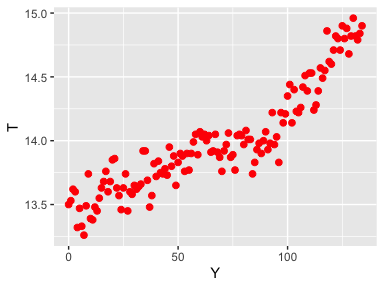
\includegraphics{series_files/figure-latex/unnamed-chunk-133-1.pdf}
\caption{\label{fig:unnamed-chunk-133}Scatterplot of global temperature data. The variable \(Y\) represents the Year since 1880 and \(T\) the temperature in degrees Celsius.}
\end{figure}

We will be working with these data to fit a function \(f(Y,\vec{\alpha})=T\). In order to fit a function in \texttt{R} we need three essential elements:

\begin{itemize}
\tightlist
\item
  We need \textbf{data} for the formula to interpret. This needs to be a two column data table, such as \texttt{global\_temperature}.
\item
  The \textbf{regression formula} we will use for the fit is given in the text \texttt{regressionFormula\ \textless{}-\ y\ \textasciitilde{}\ 1\ +\ x}. We adopt the convention that \(y\) signifies the ``dependent variable'' and \(x\) signifies the ``independent variable,'' but are \emph{named columns in a data frame}. For the \texttt{global\_temperature} dataset we would write the \texttt{regression\_formula} as \texttt{regression\_formula\ \textless{}-\ \ globalTemp\ \textasciitilde{}\ 1\ +\ yearSince1880} Said differently, what this regression formula ``does a linear regression where the factors are a constant term and one proportional to the independent variable.''
\item
  The \textbf{command} \texttt{lm} stands for \emph{l}inear \emph{m}odel. This is the main function that does our fitting procedure, where we need to specify the dataset we are using.
\end{itemize}

That's it! So if we need to do a linear regression of global temperature against year since 1880 the code to do this is the following:

\begin{Shaded}
\begin{Highlighting}[]
\NormalTok{regression\_formula }\OtherTok{\textless{}{-}}\NormalTok{  globalTemp }\SpecialCharTok{\textasciitilde{}} \DecValTok{1} \SpecialCharTok{+}\NormalTok{ yearSince1880}

\NormalTok{linear\_fit }\OtherTok{\textless{}{-}} \FunctionTok{lm}\NormalTok{(regression\_formula,}\AttributeTok{data=}\NormalTok{global\_temperature)}

\FunctionTok{summary}\NormalTok{(linear\_fit)}
\end{Highlighting}
\end{Shaded}

\begin{verbatim}
## 
## Call:
## lm(formula = regression_formula, data = global_temperature)
## 
## Residuals:
##      Min       1Q   Median       3Q      Max 
## -0.45013 -0.11632 -0.00849  0.11326  0.36865 
## 
## Coefficients:
##                Estimate Std. Error t value Pr(>|t|)    
## (Intercept)   13.358442   0.028832  463.32   <2e-16 ***
## yearSince1880  0.009601   0.000372   25.81   <2e-16 ***
## ---
## Signif. codes:  0 '***' 0.001 '**' 0.01 '*' 0.05 '.' 0.1 ' ' 1
## 
## Residual standard error: 0.1684 on 133 degrees of freedom
## Multiple R-squared:  0.8336, Adjusted R-squared:  0.8323 
## F-statistic: 666.2 on 1 and 133 DF,  p-value: < 2.2e-16
\end{verbatim}

What is printed on the console is the summary of the fit results. This summary contains a of interesting things that you would study in advanced courses in statistics, but here is what we will focus on:

\begin{itemize}
\tightlist
\item
  The estimated \emph{coefficients} of the linear regression. The column \texttt{Estimate} lists the constants in front of our regression formula \(y=a+bx\). What follows is the error on that estimate by formulas from statistics. The other additional things are statistical tests that show significance of the estimate.
\item
  One helpful thing to look at is the \textbf{Residual standard error}, which represents the overall, total effect of the differences between the model predicted values of \(\vec{y}\) and the measured values of \(\vec{y}\). The goal of linear regression is to minimize this model-data difference.
\end{itemize}

To plot the fitted equation with the regression coefficients we are going to borrow from another package called \texttt{broom}, which helps produce model output in what is called ``tidy'' data format. You can read more about broom \href{https://broom.tidymodels.org/index.html}{here}.

Since we are only going to use one or two functions from this package, I am going to refer to the functions I need with the syntax \texttt{PACKAGE\_NAME::FUNCTION}.

First we will make a data frame with the predicted coefficients from our linear model:

\begin{Shaded}
\begin{Highlighting}[]
\NormalTok{global\_temperature\_model }\OtherTok{\textless{}{-}}\NormalTok{ broom}\SpecialCharTok{::}\FunctionTok{augment}\NormalTok{(linear\_fit, }\AttributeTok{data =}\NormalTok{ global\_temperature)}

\FunctionTok{glimpse}\NormalTok{(global\_temperature\_model)}
\end{Highlighting}
\end{Shaded}

\begin{verbatim}
## Rows: 135
## Columns: 8
## $ yearSince1880 <int> 0, 1, 2, 3, 4, 5, 6, 7, 8, 9, 10, 11, 12, 13, 14, 15, 16~
## $ globalTemp    <dbl> 13.50, 13.53, 13.62, 13.60, 13.32, 13.47, 13.33, 13.26, ~
## $ .fitted       <dbl> 13.35844, 13.36804, 13.37764, 13.38725, 13.39685, 13.406~
## $ .resid        <dbl> 0.141557734, 0.161956817, 0.242355900, 0.212754983, -0.0~
## $ .hat          <dbl> 0.02930283, 0.02865412, 0.02801515, 0.02738595, 0.026766~
## $ .sigma        <dbl> 0.1686042, 0.1684612, 0.1677079, 0.1680214, 0.1689313, 0~
## $ .cooksd       <dbl> 1.098342e-02, 1.403997e-02, 3.069797e-02, 2.309589e-02, ~
## $ .std.resid    <dbl> 0.85304308, 0.97564433, 1.45949662, 1.28082181, -0.46247~
\end{verbatim}

Notice how the augment command takes the results from \texttt{linear\_fit} with the data \texttt{global\_temperature}. I like appending \texttt{\_model} to the original name of the data frame to signify that there are modeled components here to work with. There is a lot to unpack with this new data frame, but the important ones are the columns \texttt{yearSince1880} (the independent variable) and \texttt{.fitted}, which represents the fitted coefficients.

Now we are ready to graph the data along with the fitted regression line.

\begin{Shaded}
\begin{Highlighting}[]
\FunctionTok{ggplot}\NormalTok{(}\AttributeTok{data =}\NormalTok{ global\_temperature) }\SpecialCharTok{+}
  \FunctionTok{geom\_point}\NormalTok{(}\FunctionTok{aes}\NormalTok{(}\AttributeTok{x=}\NormalTok{yearSince1880,}\AttributeTok{y=}\NormalTok{globalTemp),}
             \AttributeTok{color=}\StringTok{\textquotesingle{}red\textquotesingle{}}\NormalTok{,}
             \AttributeTok{size=}\DecValTok{2}\NormalTok{) }\SpecialCharTok{+}
  \FunctionTok{geom\_line}\NormalTok{(}\AttributeTok{data =}\NormalTok{ global\_temperature\_model,}
            \FunctionTok{aes}\NormalTok{(}\AttributeTok{x=}\NormalTok{yearSince1880,}\AttributeTok{y=}\NormalTok{.fitted)) }\SpecialCharTok{+}
  \FunctionTok{labs}\NormalTok{(}\AttributeTok{x=}\StringTok{\textquotesingle{}Year Since 1880\textquotesingle{}}\NormalTok{,}
         \AttributeTok{y=}\StringTok{\textquotesingle{}Temperature (Celsius)\textquotesingle{}}\NormalTok{)}
\end{Highlighting}
\end{Shaded}

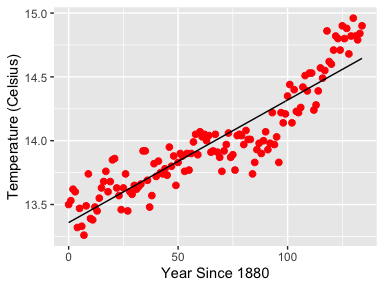
\includegraphics{series_files/figure-latex/unnamed-chunk-136-1.pdf}

\hypertarget{moving-beyond-linear-models}{%
\section{Moving beyond linear models}\label{moving-beyond-linear-models}}

We can also fit additional polynomial models such as the equation
\(y = a + bx + cx^{2} + dx^{3} ...\) (estimated parameters \(a\), \(b\), \(c\), \(d\), \ldots). There is a key distinction here: the equation is \emph{nonlinear} in the variable \(x\), but \emph{linear} with respect to the parameters. How we do that in \texttt{R} is pretty simple, it just depends on how we enter in the regression formula. Here are few templates:

\begin{longtable}[]{@{}ll@{}}
\toprule
\textbf{Equation} & \textbf{Regression Formula} \\
\midrule
\endhead
\(y=a+bx\) & \texttt{y\ \textasciitilde{}\ 1\ +\ x} \\
\(y=a\) & \texttt{y\ \textasciitilde{}\ 1} \\
\(y=bx\) & \texttt{y\ \textasciitilde{}\ -1+x} \\
\(y=a+bx+cx^{2}\) & \texttt{y\ \textasciitilde{}\ 1\ +\ x\ +\ I(x\^{}2)} \\
\(y=a+bx+cx^{2}+dx^{3}\) & \texttt{y\textasciitilde{}\ 1\ +\ x\ +\ I(x\^{}2)\ +\ I(x\^{}3)} \\
\bottomrule
\end{longtable}

Note: the structure \texttt{I(..)} is needed for \texttt{R} to signify a factor of the form \(x^{n}\).

\hypertarget{can-you-linearize-your-model}{%
\section{Can you linearize your model?}\label{can-you-linearize-your-model}}

We can also plot nonlinear models, or models that can be made linear. While the equation \(y=ae^{bx}\) non linear with respect to the parameters, it can be made linear by a \emph{logarithmic transformation} of the data:
\begin{equation}
\ln(y) = \ln(ae^{bx}) = \ln(a) + \ln (e^{bx}) = \ln(a) + bx
\end{equation}

The advantage to this approach is that the growth rate parameter is easily identifiable from the data, and the value of \(a\) is found by exponentiation of the fitted intercept value. The disadvantage is that you need to interpret the do a log transform of the \(y\) variable first before doing any fits.

\begin{example}
\protect\hypertarget{exm:unnamed-chunk-137}{}{\label{exm:unnamed-chunk-137} }A common equation in enzyme kinetics is the \emph{Michaelis-Menten} law, which states that the rate of the uptake of a substrate \(V\) is given by the equation:

\begin{equation}
V = \frac{V_{max} s}{s+K_{m}},
\end{equation}

where \(s\) is the amount of substrate, \(K_{m}\) is half-saturation constant, and \(V_{max}\) the maximum reaction rate. (Typically \(V\) is used to signify the ``velocity'' of the reaction.)

Say you have the following data:

\begin{longtable}[]{@{}ll@{}}
\toprule
\emph{s} (mM) & \emph{V} (mM / s) \\
\midrule
\endhead
0.1 & 0.04 \\
0.2 & 0.08 \\
0.5 & 0.17 \\
1.0 & 0.24 \\
2.0 & 0.32 \\
3.5 & 0.39 \\
5.0 & 0.42 \\
\bottomrule
\end{longtable}

Let's explore these data in \texttt{R}.
\end{example}

\begin{solution}
\iffalse{} {Solution. } \fi{}First thing that we will need to do is to define a data frame (\texttt{tibble}) of these data:
\end{solution}

\begin{Shaded}
\begin{Highlighting}[]
\NormalTok{enzyme\_data }\OtherTok{\textless{}{-}} \FunctionTok{tibble}\NormalTok{(}
  \AttributeTok{s =} \FunctionTok{c}\NormalTok{(}\FloatTok{0.1}\NormalTok{,}\FloatTok{0.2}\NormalTok{,}\FloatTok{0.5}\NormalTok{,}\FloatTok{1.0}\NormalTok{,}\FloatTok{2.0}\NormalTok{,}\FloatTok{3.5}\NormalTok{,}\FloatTok{5.0}\NormalTok{),}
  \AttributeTok{V =} \FunctionTok{c}\NormalTok{(}\FloatTok{0.04}\NormalTok{,}\FloatTok{0.08}\NormalTok{,}\FloatTok{0.17}\NormalTok{,}\FloatTok{0.24}\NormalTok{,}\FloatTok{0.32}\NormalTok{,}\FloatTok{0.39}\NormalTok{,}\FloatTok{0.42}\NormalTok{) )}
\end{Highlighting}
\end{Shaded}

Next let's do some exploratory data analysis:

\begin{Shaded}
\begin{Highlighting}[]
\FunctionTok{ggplot}\NormalTok{(}\AttributeTok{data =}\NormalTok{ enzyme\_data) }\SpecialCharTok{+}
  \FunctionTok{geom\_point}\NormalTok{(}\FunctionTok{aes}\NormalTok{(}\AttributeTok{x=}\NormalTok{s,}\AttributeTok{y=}\NormalTok{V),}
             \AttributeTok{color=}\StringTok{\textquotesingle{}red\textquotesingle{}}\NormalTok{,}
             \AttributeTok{size=}\DecValTok{2}\NormalTok{) }\SpecialCharTok{+}
  \FunctionTok{labs}\NormalTok{(}\AttributeTok{x =} \StringTok{\textquotesingle{}s (mM)\textquotesingle{}}\NormalTok{,}
       \AttributeTok{y=} \StringTok{\textquotesingle{}V (mM / s)\textquotesingle{}}\NormalTok{)}
\end{Highlighting}
\end{Shaded}

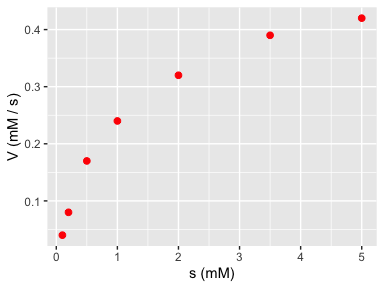
\includegraphics{series_files/figure-latex/unnamed-chunk-140-1.pdf}

Definitely looks non-linear. But take a look at what happens if we plot the reciprocal of \(s\) and the reciprocal of \(V\):

\begin{Shaded}
\begin{Highlighting}[]
\FunctionTok{ggplot}\NormalTok{(}\AttributeTok{data =}\NormalTok{ enzyme\_data) }\SpecialCharTok{+}
  \FunctionTok{geom\_point}\NormalTok{(}\FunctionTok{aes}\NormalTok{(}\AttributeTok{x=}\DecValTok{1}\SpecialCharTok{/}\NormalTok{s,}\AttributeTok{y=}\DecValTok{1}\SpecialCharTok{/}\NormalTok{V),}
             \AttributeTok{color=}\StringTok{\textquotesingle{}red\textquotesingle{}}\NormalTok{,}
             \AttributeTok{size=}\DecValTok{2}\NormalTok{) }\SpecialCharTok{+}
  \FunctionTok{labs}\NormalTok{(}\AttributeTok{x =} \StringTok{\textquotesingle{}1/s (1/mM)\textquotesingle{}}\NormalTok{,}
       \AttributeTok{y=} \StringTok{\textquotesingle{}1/V (s / mM)\textquotesingle{}}\NormalTok{)}
\end{Highlighting}
\end{Shaded}

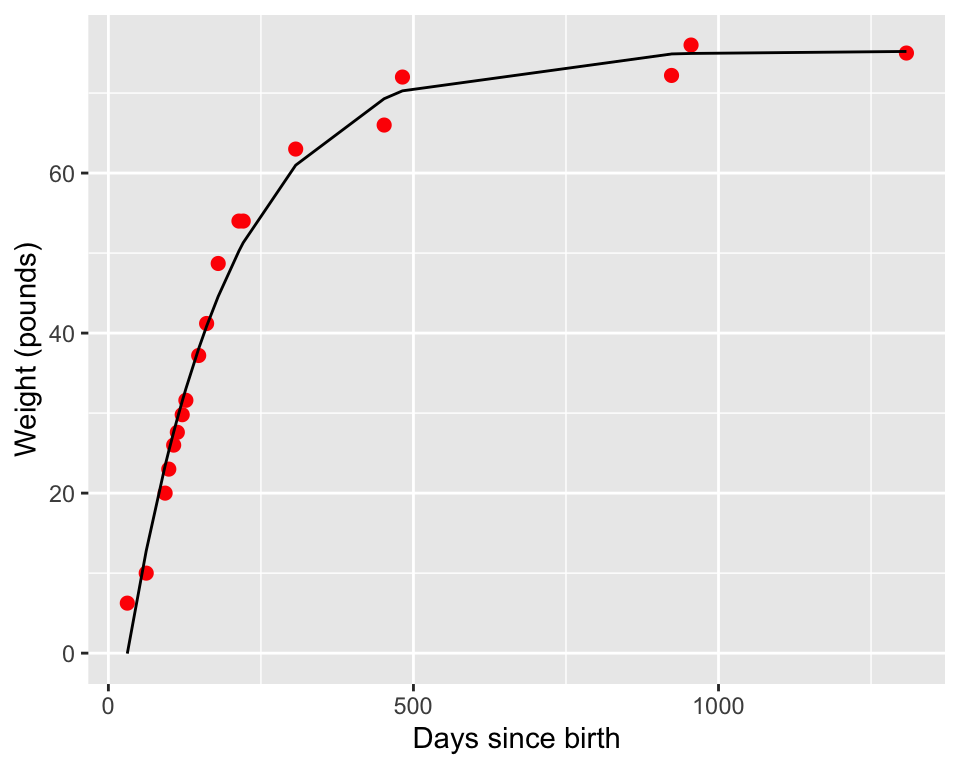
\includegraphics{series_files/figure-latex/unnamed-chunk-141-1.pdf}
That looks really linear! Notice how easy it was to do that data transformation in our plot command. In order to do a linear fit to the transformed data we will use the regression formulas defined above and the handy structure \texttt{I(VARIABLE)}:

\begin{Shaded}
\begin{Highlighting}[]
\NormalTok{enzyme\_fit }\OtherTok{\textless{}{-}} \FunctionTok{lm}\NormalTok{(}\FunctionTok{I}\NormalTok{(}\DecValTok{1}\SpecialCharTok{/}\NormalTok{V) }\SpecialCharTok{\textasciitilde{}} \DecValTok{1}\SpecialCharTok{+} \FunctionTok{I}\NormalTok{(}\DecValTok{1}\SpecialCharTok{/}\NormalTok{s), }
              \AttributeTok{data =}\NormalTok{ enzyme\_data)}


\FunctionTok{summary}\NormalTok{(enzyme\_fit)}
\end{Highlighting}
\end{Shaded}

\begin{verbatim}
## 
## Call:
## lm(formula = I(1/V) ~ 1 + I(1/s), data = enzyme_data)
## 
## Residuals:
##       1       2       3       4       5       6       7 
##  0.3913 -0.6764 -0.4347  0.1360  0.2376  0.1667  0.1795 
## 
## Coefficients:
##             Estimate Std. Error t value Pr(>|t|)    
## (Intercept)  1.74417    0.21009   8.302 0.000414 ***
## I(1/s)       2.28645    0.04868  46.968 8.26e-08 ***
## ---
## Signif. codes:  0 '***' 0.001 '**' 0.01 '*' 0.05 '.' 0.1 ' ' 1
## 
## Residual standard error: 0.4323 on 5 degrees of freedom
## Multiple R-squared:  0.9977, Adjusted R-squared:  0.9973 
## F-statistic:  2206 on 1 and 5 DF,  p-value: 8.263e-08
\end{verbatim}

\begin{Shaded}
\begin{Highlighting}[]
\NormalTok{enzyme\_data\_model }\OtherTok{\textless{}{-}}\NormalTok{ broom}\SpecialCharTok{::}\FunctionTok{augment}\NormalTok{(enzyme\_fit,}\AttributeTok{data=}\NormalTok{enzyme\_data)}

\FunctionTok{ggplot}\NormalTok{(}\AttributeTok{data =}\NormalTok{ enzyme\_data) }\SpecialCharTok{+}
  \FunctionTok{geom\_point}\NormalTok{(}\FunctionTok{aes}\NormalTok{(}\AttributeTok{x=}\DecValTok{1}\SpecialCharTok{/}\NormalTok{s,}\AttributeTok{y=}\DecValTok{1}\SpecialCharTok{/}\NormalTok{V),}
             \AttributeTok{color=}\StringTok{\textquotesingle{}red\textquotesingle{}}\NormalTok{,}
             \AttributeTok{size=}\DecValTok{2}\NormalTok{) }\SpecialCharTok{+}
  \FunctionTok{geom\_line}\NormalTok{(}\AttributeTok{data =}\NormalTok{ enzyme\_data\_model,}
            \FunctionTok{aes}\NormalTok{(}\AttributeTok{x=}\DecValTok{1}\SpecialCharTok{/}\NormalTok{s,}\AttributeTok{y=}\NormalTok{.fitted)) }\SpecialCharTok{+}
  \FunctionTok{labs}\NormalTok{(}\AttributeTok{x =} \StringTok{\textquotesingle{}1/s (1/mM)\textquotesingle{}}\NormalTok{,}
       \AttributeTok{y=} \StringTok{\textquotesingle{}1/V (s / mM)\textquotesingle{}}\NormalTok{)}
\end{Highlighting}
\end{Shaded}

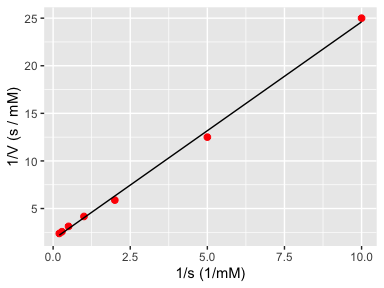
\includegraphics{series_files/figure-latex/unnamed-chunk-142-1.pdf}

Notice when plotting the fitted model we didn't need to take the reciprocal of \texttt{.fitted} because the linear model already did the inverse. However if we wanted to plot the model with the original data, then we need to take the reciprocal (confusing - I know!)

\begin{Shaded}
\begin{Highlighting}[]
\FunctionTok{ggplot}\NormalTok{(}\AttributeTok{data =}\NormalTok{ enzyme\_data) }\SpecialCharTok{+}
  \FunctionTok{geom\_point}\NormalTok{(}\FunctionTok{aes}\NormalTok{(}\AttributeTok{x=}\NormalTok{s,}\AttributeTok{y=}\NormalTok{V),}
             \AttributeTok{color=}\StringTok{\textquotesingle{}red\textquotesingle{}}\NormalTok{,}
             \AttributeTok{size=}\DecValTok{2}\NormalTok{) }\SpecialCharTok{+}
  \FunctionTok{geom\_line}\NormalTok{(}\AttributeTok{data =}\NormalTok{ enzyme\_data\_model,}
            \FunctionTok{aes}\NormalTok{(}\AttributeTok{x=}\NormalTok{s,}\AttributeTok{y=}\DecValTok{1}\SpecialCharTok{/}\NormalTok{.fitted)) }\SpecialCharTok{+}
  \FunctionTok{labs}\NormalTok{(}\AttributeTok{x =} \StringTok{\textquotesingle{}s (mM)\textquotesingle{}}\NormalTok{,}
       \AttributeTok{y=} \StringTok{\textquotesingle{}V (mM / s)\textquotesingle{}}\NormalTok{)}
\end{Highlighting}
\end{Shaded}

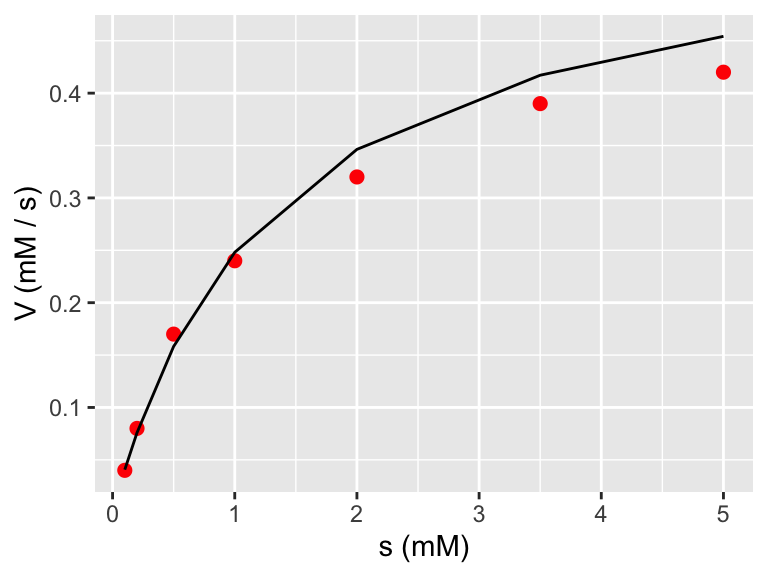
\includegraphics{series_files/figure-latex/unnamed-chunk-143-1.pdf}

\hypertarget{nonlinear-models}{%
\section{Nonlinear models}\label{nonlinear-models}}

Many cases you will not be able to write your model in a linear format. You can still do a non-linear curve fit using the function \texttt{nlm}, however you will need to specify the function along with the formula you are using. For example if we try to fit the weight of the dog Wilson over time to the logistic equation we would have the following:

\begin{equation}
W =f(D,a,b,c)= a - be^{ct},
\end{equation}

where we have the parameters \(a\), \(b\), and \(c\). Notice how \(W\) is a function of \(D\) and the parameters.

\begin{Shaded}
\begin{Highlighting}[]
\NormalTok{nonlinear\_fit }\OtherTok{\textless{}{-}} \FunctionTok{nls}\NormalTok{(mass }\SpecialCharTok{\textasciitilde{}}\NormalTok{ a}\SpecialCharTok{{-}}\NormalTok{b}\SpecialCharTok{*}\FunctionTok{exp}\NormalTok{(c}\SpecialCharTok{*}\NormalTok{days), }
              \AttributeTok{data =}\NormalTok{ wilson, }
              \AttributeTok{start =} \FunctionTok{list}\NormalTok{(}\AttributeTok{a =} \DecValTok{75}\NormalTok{, }\AttributeTok{b =} \DecValTok{30}\NormalTok{,}\AttributeTok{c =} \SpecialCharTok{{-}}\FloatTok{0.01}\NormalTok{))}


\FunctionTok{summary}\NormalTok{(nonlinear\_fit)}
\end{Highlighting}
\end{Shaded}

\begin{verbatim}
## 
## Formula: mass ~ a - b * exp(c * days)
## 
## Parameters:
##     Estimate Std. Error t value Pr(>|t|)    
## a 75.2349873  1.5726835   47.84  < 2e-16 ***
## b 90.7696994  3.3999731   26.70 1.07e-14 ***
## c -0.0060311  0.0004324  -13.95 2.26e-10 ***
## ---
## Signif. codes:  0 '***' 0.001 '**' 0.01 '*' 0.05 '.' 0.1 ' ' 1
## 
## Residual standard error: 2.961 on 16 degrees of freedom
## 
## Number of iterations to convergence: 11 
## Achieved convergence tolerance: 6.9e-06
\end{verbatim}

The tricky part for a nonlinear model is that you need a starting value for the parameters (it is an iterative method). This can be tricky and takes some trial and error.

However once you have your fitted model, you can still plot the fitted values with the coefficients:

\begin{Shaded}
\begin{Highlighting}[]
\NormalTok{wilson\_model }\OtherTok{\textless{}{-}}\NormalTok{ broom}\SpecialCharTok{::}\FunctionTok{augment}\NormalTok{(nonlinear\_fit, }\AttributeTok{data =}\NormalTok{ wilson)}

\FunctionTok{ggplot}\NormalTok{(}\AttributeTok{data =}\NormalTok{ wilson) }\SpecialCharTok{+}
  \FunctionTok{geom\_point}\NormalTok{(}\FunctionTok{aes}\NormalTok{(}\AttributeTok{x=}\NormalTok{days,}\AttributeTok{y=}\NormalTok{mass),}
             \AttributeTok{color=}\StringTok{\textquotesingle{}red\textquotesingle{}}\NormalTok{,}
             \AttributeTok{size=}\DecValTok{2}\NormalTok{) }\SpecialCharTok{+}
  \FunctionTok{geom\_line}\NormalTok{(}\AttributeTok{data =}\NormalTok{ wilson\_model,}
            \FunctionTok{aes}\NormalTok{(}\AttributeTok{x=}\NormalTok{days,}\AttributeTok{y=}\NormalTok{.fitted)) }\SpecialCharTok{+}
  \FunctionTok{labs}\NormalTok{(}\AttributeTok{x=}\StringTok{\textquotesingle{}Days since birth\textquotesingle{}}\NormalTok{,}
         \AttributeTok{y=}\StringTok{\textquotesingle{}Weight (pounds)\textquotesingle{}}\NormalTok{)}
\end{Highlighting}
\end{Shaded}

\includegraphics{series_files/figure-latex/unnamed-chunk-145-1.pdf}

We will revisit these data later when we are making likelihood functions.

\newpage

\hypertarget{exercises-7}{%
\section{Exercises}\label{exercises-7}}

\begin{exercise}
\protect\hypertarget{exr:unnamed-chunk-146}{}{\label{exr:unnamed-chunk-146} }Determine if the following equations are linear with respect to the parameters. For the purposes of this problem we assume that \(y\) is a function of \(x\).

\begin{enumerate}[label=\alph*.]
\item $y=a + bx+cx^{2}+dx^{3}$
\item $y=a \sin (x) + b \cos (x)$
\item $y = a \sin(bx) + c \cos(dx)$
\item $y = a + bx + a\cdot b x^{2}$
\item $y = a e^{-x} + b e^{x}$
\item $y = a e^{-bx} + c e^{-dx}$
\end{enumerate}
\end{exercise}

~
\begin{exercise}
\protect\hypertarget{exr:unnamed-chunk-147}{}{\label{exr:unnamed-chunk-147} }Each of the following equations can be written as linear with respect to the parameters, through applying some elementary transformations to the data. Write each equation as a linear function with respect to the parameters.

\begin{enumerate}[label=\alph*.]
\item $y=ae^{-bx}$
\item $y=(a+bx)^{2}$
\item $\displaystyle y =  \frac{1}{a+bx}$
\item $y = c x^{n}$
\end{enumerate}
\end{exercise}

~

\begin{exercise}
\protect\hypertarget{exr:unnamed-chunk-148}{}{\label{exr:unnamed-chunk-148} }Use the dataset \texttt{global\_temperature} and the function \texttt{lm} to answer the following questions:

\begin{enumerate}[label=\alph*.]
\item Complete the following table, which represents various regression fits to global temperature $T$ (in degrees Celsius) and years since 1880 (denoted by $Y$). In the table \textbf{Coeffiicients} represent the values of the parameters $a$, $b$, $c$, etc from your fitted equation; \textbf{P} =  number of parameters; \textbf{RSE} = Residual standard error.

\begin{tabular}{l|c|c|c}
\textbf{Equation} & \textbf{Coefficients} & \textbf{P} & \textbf{RSE} \\ \hline
     $T=a+bY$ &&& \\
    $T=a+bY+cY^{2}$ &&& \\
     $T=a+bY+cY^{2}+dY^{3}$ &&& \\
     $T=a+bY+cY^{2}+dY^{3}+eY^{4}$ &&& \\
   $T=a+bY+cY^{2}+dY^{3}+eY^{4}+fY^{5}$ &&& \\
      $T=a+bY+cY^{2}+dY^{3}+eY^{4}+fY^{5}+gY^{6}$ &&&
\end{tabular}

\item After making this table, choose the polynomial of the function that you believe fits the data best.  Provide reasoning and explanation why you chose the polynomial that you did.
\item Finally show the plot of your selected polynomial with the data.
\end{enumerate}
\end{exercise}

~
\begin{exercise}
\protect\hypertarget{exr:log-linear-08}{}{\label{exr:log-linear-08} }An equation that relates a consumer's nutrient content (denoted as \(y\)) to the nutrient content of food (denoted as \(x\)) is given by: \(\displaystyle y = c x^{1/\theta},\) where \(\theta \geq 1\) and \(c\) are both constants is a constant.

\begin{enumerate}[label=\alph*.]
\item Show that you can write this equation as linear equation by applying a logarithm to both sides and simplifying.
\item Use the dataset `phosphorous` to determine a linear regression fit for your new linear equation.
\item Determine the value of $c$ and $\theta$ in the original equation with the parameters from the linear fit.
\end{enumerate}
\end{exercise}

~

\begin{exercise}
\protect\hypertarget{exr:unnamed-chunk-149}{}{\label{exr:unnamed-chunk-149} }Following on from the last exercise, do a non-linear least squares fit for the dataset \texttt{phosphorous} to the equation \(\displaystyle y = c x^{1/\theta},\) where \(\theta \geq 1\) and \(c\) are both constants is a constant. For a starting point, you may use the values of \(c\) and \(\theta\) from the previous exercise. Finally make a plot of the original phosophorous data and the fitted model.
\end{exercise}
~

\begin{exercise}
\protect\hypertarget{exr:unnamed-chunk-150}{}{\label{exr:unnamed-chunk-150} }A common equation in enzyme kinetics is the \emph{Michaelis-Menten} law, which states that the rate of the uptake of a substrate \(V\) is given by the equation:

\begin{equation}
V = \frac{V_{max} s}{s+K_{m}},
\end{equation}

where \(s\) is the amount of substrate, \(K_{m}\) is half-saturation constant, and \(V_{max}\) the maximum reaction rate. (Typically \(V\) is used to signify the ``velocity'' of the reaction.)

Say you have the following data:

\begin{longtable}[]{@{}ll@{}}
\toprule
\emph{s} (mM) & \emph{V} (mM / s) \\
\midrule
\endhead
0.1 & 0.04 \\
0.2 & 0.08 \\
0.5 & 0.17 \\
1.0 & 0.24 \\
2.0 & 0.32 \\
3.5 & 0.39 \\
5.0 & 0.42 \\
\bottomrule
\end{longtable}

\begin{enumerate}[label=\alph*.]
\item Using algebra, show that this equation can be written as $\displaystyle \frac{1}{V} = \frac{1}{V_{max}} + \frac{K_{m}}{V_{max}} \cdot \frac{1}{s}$
\item  The text determined the fitted coefficients for these transformed data.  Determine values of $K_{m}$ and $V_{max}$.
\item Make a plot of the actual data to the fitted model curve you found.
\end{enumerate}

\emph{Note:} The process outlined here is a \emph{Lineweaver-Burk} plot.
\end{exercise}
~

\begin{exercise}
\protect\hypertarget{exr:unnamed-chunk-151}{}{\label{exr:unnamed-chunk-151} }Following on from the last exercise, let's do a nonlinear least squares fit of the enzyme data to the equation:

\begin{equation}
V = \frac{V_{max} s}{s+K_{m}},
\end{equation}

where \(s\) is the amount of substrate, \(K_{m}\) is half-saturation constant, and \(V_{max}\) the maximum reaction rate.

\begin{enumerate}[label=\alph*.]
\item Determine a non-linear least squares fit to the data for the given equation.  You may use the values of $K_{m}$ and $V_{max}$ that you determined in the last exercise.
\item Make a plot of the actual data to the fitted model curve you found.
\end{enumerate}
\end{exercise}

~

\begin{exercise}
\protect\hypertarget{exr:unnamed-chunk-152}{}{\label{exr:unnamed-chunk-152} }
Consider the following data which represents the temperature over the course of a day:

\begin{tabular}{lccccccccccccc}
\textbf{Hour} & 0 & 1 & 2 & 3 & 4 & 5 & 6 & 7 & 8 & 9 &10 &11 &12  \\ \hline
\textbf{Temperature} ($^{\circ}$F) 
& 54 &53 &55& 54& 58& 58 &61& 63 &67& 66& 67& 69& 68 \\ \hline \hline
\textbf{Hour} &13 &14 &15 &16 &17 &18 &19 &20& 21& 22& 23& 24 & \\
\textbf{Temperature} ($^{\circ}$F) &
 68& 66& 67& 63& 60& 59& 57& 56& 53& 52& 54& 53 & \\ \hline
\end{tabular}

\begin{enumerate}[label=\alph*.]
\item Make a scatterplot of these data, with the variable \textbf{Hour} on the horizontal axis.
\item A function that describes these data is $\displaystyle T = A + B \sin \left( \frac{\pi}{12} \cdot H \right) + C \cos \left( \frac{\pi}{12} \cdot H \right)$, where $H$ is the hour and $T$ is the temperature.  Explain why this equation is linear for the parameters $A$, $B$, and $C$.
\item Define a \texttt{tibble} that include the variables $T$, $\displaystyle \sin \left( \frac{\pi}{12} \cdot H \right)$ $\displaystyle \cos \left( \frac{\pi}{12} \cdot H \right)$.
\item Do a linear fit on your new data frame to report the values of $A$, $B$, and $C$.
\item Add your fitted curve to the scatterplot.
\end{enumerate}
\end{exercise}

\hypertarget{likelihood-09}{%
\chapter{Probability and Likelihood Functions}\label{likelihood-09}}

The problem we examined in the last chapter was the following:

\begin{quote}
Determine the set of parameters \(\vec{\alpha}\) that minimize the difference between data \(\vec{y}\) and the output of the function \(f(\vec{x}, \vec{\alpha})\) and measured error \(\vec{\sigma}\).
\end{quote}

We are going to examine the linear regression problem again using a smaller dataset. Ohe to the linear regression problem is through \emph{likelihood functions}, which is a topic from probability and statistics.

This section will introduce likelihood functions but also discuss some interesting visualization techniques of multivariable functions and contour plots. We will also see a technique to evaluate a continuous function. We are starting to build out some R skills and techniques that you can apply in other context. Let's get started!

\hypertarget{linear-regression-part-2}{%
\section{Linear regression, part 2}\label{linear-regression-part-2}}

Assume we have the following (limited) number of points where we wish to fit a function of the form \(y=bx\).

\begin{longtable}[]{@{}cc@{}}
\toprule
\emph{x} & \emph{y} \\
\midrule
\endhead
1 & 3 \\
2 & 5 \\
4 & 4 \\
4 & 10 \\
\bottomrule
\end{longtable}

For this example we are forcing the intercept term \(a\) to equal zero - for most cases you will just fit the linear equation. See Exercise \ref{exr:full-linear}. Figure \ref{fig:quick-scatter-07} displays a quick scatterplot of these data:

\begin{figure}
\centering
\includegraphics{series_files/figure-latex/quick-scatter-07-1.pdf}
\caption{\label{fig:quick-scatter-07}A scatterplot of a small dataset.}
\end{figure}

The goal here is to work to determine the value of \(b\) that is most \emph{likely} (in other words, consistent) with the data. In order to do this, we need to take a quick excursion into probability distributions. Let's go!

\hypertarget{probability}{%
\section{Probability}\label{probability}}

In order to understand likelihood functions, first I am going to review very essential information about probability and probability distributions. Probability is the association of a set of observable events to a quantitative scale between 0 to 1. (Zero means that event is not possible, 1 means that it definitely can happen). This definition could be refined somewhat (\protect\hyperlink{ref-devore_modern_2021}{\textbf{devore\_modern\_2021?}}). You can consider discrete events (think counting or combinatorial problems) or continuous events. Here we are only going to consider continuous events, specifically in this case the probability of a parameter obtaining a particular value.

Consider this graphic, which may be familiar to you as the normal distribution or the bell curve:

\begin{figure}
\centering
\includegraphics{series_files/figure-latex/unnamed-chunk-153-1.pdf}
\caption{\label{fig:unnamed-chunk-153}The normal distribution}
\end{figure}

We tend to think of the plot and the associated function \(f(x)\) as something with input and output (such as \(f(0)=\) 0.3989). However because it is a probability density function, the \emph{area} between two points gives yields the probability of an event to fall within two values:

\begin{figure}
\centering
\includegraphics{series_files/figure-latex/unnamed-chunk-154-1.pdf}
\caption{\label{fig:unnamed-chunk-154}The area between two values, normally distributed}
\end{figure}

In this case, the shaded area tells us the probability that our measurement is between \(x=-0.1\) and \(x=0.1\). The value of the area, or the probability is 0.07966. When you took calculus the area was expressed as a definite integral: \(\displaystyle \int_{-0.1}^{0.1} f(x) \; dx=\) 0.07966, where \(f(x)\) is the formula for the probability density function for the normal distribution.

The basic idea is that we can assign values to an outcomes as a way of displaying our belief (confidence) in the result. With this intuition we can summarize key facts about probability density functions:

\begin{itemize}
\tightlist
\item
  \(f(x) \geq 0\) (this means that probability density functions are positive values)
\item
  Area integrates to one (in probability, this means we have accounted for all of our outcomes)
\end{itemize}

The formula for the normal distribution is
\begin{equation}
f(x)=\frac{1}{\sqrt{2 \pi} \sigma } e^{-(x-\mu)^{2}/(2 \sigma^{2})}
\end{equation}

Where \(\mu\) is the mean and \(\sigma\) is the standard deviation

\hypertarget{other-probability-distributions}{%
\subsection{Other probability distributions}\label{other-probability-distributions}}

Beyond the normal distribution some of the more common ones we utilize in the parameter estimation are the following:

\begin{itemize}
\tightlist
\item
  \textbf{Uniform:} For this distribution we must specify between a minimum value \(a\) and maximum value \(b\).
\end{itemize}

\begin{figure}
\centering
\includegraphics{series_files/figure-latex/unnamed-chunk-155-1.pdf}
\caption{\label{fig:unnamed-chunk-155}The uniform distribution}
\end{figure}

The formula for the uniform distribution is
\begin{equation}
f(x)=\frac{1}{b-a} \mbox{ for } a \leq x \leq b
\end{equation}

\begin{itemize}
\tightlist
\item
  \textbf{Exponential:} For this distribution we must specify between a rate parameter \(\lambda\).
\end{itemize}

\begin{figure}
\centering
\includegraphics{series_files/figure-latex/unnamed-chunk-156-1.pdf}
\caption{\label{fig:unnamed-chunk-156}The exponential distribution}
\end{figure}

The formula for the exponential distribution is
\begin{equation}
f(x)=\lambda e^{-\lambda x} \mbox{ for } x \geq 0 
\end{equation}

where \(\lambda\) is the rate parameter

\begin{itemize}
\tightlist
\item
  \textbf{Lognormal:} This distirbution is for positive values, with mean \(\mu\) and standard deviation \(\sigma\).
\end{itemize}

\begin{figure}
\centering
\includegraphics{series_files/figure-latex/unnamed-chunk-157-1.pdf}
\caption{\label{fig:unnamed-chunk-157}The lognormal distribution}
\end{figure}

The formula for the lognormal distribution is
\begin{equation}
f(x)=\frac{1}{\sqrt{2 \pi} \sigma x } e^{-(\ln(x)-\mu)^{2}/(2 \sigma^{2})} \mbox{ for } x \geq 0 
\end{equation}

\hypertarget{computing-probabilities-in-r}{%
\subsection{Computing probabilities in R}\label{computing-probabilities-in-r}}

Here is the good news with \texttt{R}: the commands to generate densities and cumulative distributions are already included! There are a variety of implementations: both for the density, cumulative distribution, random number generation, and lognormal distributions from these. For the moment, Table \ref{table:prob-dist} summarizes some common probability distributions in \texttt{R}.

\begin{table}
\begin{tabular}{c|c|c|c}
Distribution & Key Parameters & R command & Density Example \\ \hline
Normal & $\mu \rightarrow$ \texttt{mean}, $\sigma \rightarrow$ \texttt{sd} & \texttt{norm} 
& \texttt{dnorm(mu=0,sd=1,seq(-5,5,length=200))} \\
Uniform & $a \rightarrow$ \texttt{min}, $b \rightarrow$ \texttt{max} & \texttt{unif} & \texttt{dunif(seq(-5,5,length=200),min = -5,max=5)} \\
Exponential & $\lambda \rightarrow$ \texttt{rate} & \texttt{exp} & \texttt{dexp(seq(0,5,length=200))} \\
Normal & $\mu \rightarrow$ \texttt{meanlog}, $\sigma \rightarrow$ \texttt{sdlog} & \texttt{lnorm} 
& \texttt{dlnorm(seq(0,5,length=200))}
\end{tabular}
\caption{Summary of common probability distributions in \texttt{R}}\label{table:prob-dist}
\end{table}

To make the graphs of these density functions in \texttt{R} we use the prefix \texttt{d\ +} the name (\texttt{norm}, \texttt{exp}) etc of the distribution we wish to specify, including any of the key parameters. If we don't include any of the parameters then it will just use the defaults (which you can see by typing \texttt{?NAME} where \texttt{NAME} is the name of the command (i.e.~\texttt{?dnorm}).

Here is some sample code to plot the lognormal distribution:

\begin{example}
\protect\hypertarget{exm:unnamed-chunk-158}{}{\label{exm:unnamed-chunk-158} }Make a graph of the lognormal density function with \(\mu=0\) and \(\sigma=1\) from \(0 \leq x \leq 5\).
\end{example}

\begin{remark}
\iffalse{} {Remark. } \fi{}For this case we are using the defaults of the lognormal distribution. The code is the following, and plotted in Figure \ref{fig:log-norm-plot}.
\end{remark}

\begin{Shaded}
\begin{Highlighting}[]
\NormalTok{x }\OtherTok{\textless{}{-}} \FunctionTok{seq}\NormalTok{(}\DecValTok{0}\NormalTok{,}\DecValTok{5}\NormalTok{,}\AttributeTok{length=}\DecValTok{200}\NormalTok{)}
\NormalTok{y }\OtherTok{\textless{}{-}} \FunctionTok{dlnorm}\NormalTok{(x)  }\CommentTok{\# Just use the mean defaults }

\NormalTok{lognormal\_data }\OtherTok{\textless{}{-}} \FunctionTok{tibble}\NormalTok{(x,y)}

\FunctionTok{ggplot}\NormalTok{() }\SpecialCharTok{+}
  \FunctionTok{geom\_line}\NormalTok{(}\AttributeTok{data =}\NormalTok{ lognormal\_data,}
             \FunctionTok{aes}\NormalTok{(}\AttributeTok{x=}\NormalTok{x,}\AttributeTok{y=}\NormalTok{y)) }\SpecialCharTok{+}
  \FunctionTok{labs}\NormalTok{(}\AttributeTok{x =} \StringTok{\textquotesingle{}x\textquotesingle{}}\NormalTok{, }\AttributeTok{y=} \StringTok{\textquotesingle{}Lognormal density\textquotesingle{}}\NormalTok{)}
\end{Highlighting}
\end{Shaded}

\begin{figure}
\centering
\includegraphics{series_files/figure-latex/log-norm-plot-1.pdf}
\caption{\label{fig:log-norm-plot}Code to plot the lognormal distribution}
\end{figure}

To find the area between two values in a density function we use the prefix \texttt{p}.

\begin{example}
\protect\hypertarget{exm:exp-area}{}{\label{exm:exp-area} }Use \texttt{R} to evaluate \(\displaystyle \int_{1}^{2} e^{-x} \; dx\).
\end{example}

\begin{remark}
\iffalse{} {Remark. } \fi{}The function \(e^{-x}\) is the exponential probability distribution with \(\lambda=1\). For this example if we wanted to find the area between two values in the exponential density in the shaded graph we would type \texttt{pexp(2)-pexp(1)} at the \texttt{R} console, which would give the value of \texttt{r\ round(pexp(2)-pexp(1),digits=3)}. A visual representation of this area is shown in Figure \ref{fig:exp-area-plot}.
\end{remark}

\begin{figure}
\centering
\includegraphics{series_files/figure-latex/exp-area-plot-1.pdf}
\caption{\label{fig:exp-area-plot}The area for the exponential distribution}
\end{figure}

\hypertarget{connecting-to-linear-regression}{%
\section{Connecting to linear regression}\label{connecting-to-linear-regression}}

Now that we have made that small excursion into probablity, let's start to return back to the linear regression problem. Another way to phrase this the linear regression problem studied in the last chapter is to examine the probability distribution of the model-data residual \(\epsilon\):

\begin{equation}
\epsilon_{i} = y_{i} - f(x_{i},\vec{\alpha} ).
\end{equation}

The approach with likelihood functions assumes a particular probability distribution on each residual. One common assumption is that the residual \emph{distribution} is normal with mean \(\mu=0\) and standard deviation \(\sigma\) (which could be specified as measurement error, etc).

\begin{equation}
L(\epsilon_{i}) = \frac{1}{\sqrt{2 \pi} \sigma} e^{-\epsilon_{i}^{2} / 2 \sigma^{2} },
\end{equation}

To extend this further across all measurement, we use the idea of \emph{independent, identically distributed} measurements so the joint likelihood of \textbf{all} the residuals is the product of the likelihoods

\begin{equation}
L(\vec{\epsilon}) = \prod_{i=1}^{N} \frac{1}{\sqrt{2 \pi} \sigma} e^{-\epsilon_{i}^{2} / 2 \sigma^{2} },
\end{equation}

We are making progress here, but in order to fully characterize the solution we need to specify the parameters \(\vec{\alpha}\). A simple redefining of the likelihood function where we specify the measurements (\(x\) and \(y\)) and parameters (\(\vec{\alpha}\)) is all we need:

\begin{equation}
L(\vec{\alpha} | \vec{x},\vec{y} )= \prod_{i=1}^{N}  \frac{1}{\sqrt{2 \pi} \sigma} \exp(-(y_{i} - f(x_{i},\vec{\alpha} ))^{2} / 2 \sigma^{2} )  
\end{equation}

Now we have a function where the best parameter estimate is the one that optimizes the likelihood.

To get back to our original linear regression problem. As a reminder we wanted to fit the function \(y=bx\) to the following set of points:

\begin{longtable}[]{@{}cc@{}}
\toprule
\emph{x} & \emph{y} \\
\midrule
\endhead
1 & 3 \\
2 & 5 \\
4 & 4 \\
4 & 10 \\
\bottomrule
\end{longtable}

The likelihood \(L(\epsilon_{i}) ~ N(0,\sigma)\) characterizing these data are the following:

\begin{equation}
L(b) = \left( \frac{1}{\sqrt{2 \pi} \sigma}\right)^{4} e^{-\frac{(3-b)^{2}}{2\sigma}} \cdot e^{-\frac{(5-2b)^{2}}{2\sigma}}  \cdot e^{-\frac{(4-4b)^{2}}{2\sigma}}  \cdot e^{-\frac{(10-4b)^{2}}{2\sigma}} \label{eq:small-data-likely}
\end{equation}

For the purposes of our argument here, we will assume \(\sigma=1\). Let's also make a plot of this likelihood function:

\begin{figure}
\centering
\includegraphics{series_files/figure-latex/small-likelihood-plot-1.pdf}
\caption{\label{fig:small-likelihood-plot}The likelihood function for the small dataset}
\end{figure}

Note that although the \(y\) values of the likelihood function are really small, the likelihood function is maximized at \(b=1.86\).

Notice how in the plot of our likelihood function we had really small values of \(L(b)\). It is also common to use the log likelihood (Equation \eqref{eq:loglikely}:

\begin{equation}
\begin{split}
\ln(L(\vec{\alpha} | \vec{x},\vec{y} )) &=  N \ln \left( \frac{1}{\sqrt{2 \pi} \sigma} \right) - \sum_{i=1}^{N} \frac{ (y_{i} - f(x_{i},\vec{\alpha} )^{2}}{ 2 \sigma^{2}} \\
 & = - \frac{N}{2} \ln (2) - \frac{N}{2} \ln(\pi) - N \ln( \sigma) - \sum_{i=1}^{N} \frac{ (y_{i} - f(x_{i},\vec{\alpha} )^{2}}{ 2 \sigma^{2}}
\end{split} \label{eq:loglikely}
\end{equation}

In the homework you will be working on how to transform the likelihood function \(L(b)\) to the log-likelihood \(\ln(L(b))\).

For our purposes here we are going to assume independent, identical, normally distributed errors with a mean 0 for the likelihood functions. This is a commonly used assumption for this approach, but you should always think about the errors in more advanced applications.

\hypertarget{plotting-likelihood-surfaces}{%
\section{Plotting likelihood surfaces}\label{plotting-likelihood-surfaces}}

Ok, we are going to examine a second example from (\protect\hyperlink{ref-gause_experimental_1932}{\textbf{gause\_experimental\_1932?}}) which modeled the growing of yeast in solution. This classic paper examines the biological principal of \emph{competitive exclusion}, how one species can out compete another one for resources. For our purposes here we are going to examine a model for one species growing without competition.

First let's make a quick plot of the function:

\begin{Shaded}
\begin{Highlighting}[]
\DocumentationTok{\#\#\# Make a quick ggplot of the data}

\FunctionTok{ggplot}\NormalTok{() }\SpecialCharTok{+}
  \FunctionTok{geom\_point}\NormalTok{(}\AttributeTok{data =}\NormalTok{ yeast,}
             \FunctionTok{aes}\NormalTok{(}\AttributeTok{x=}\NormalTok{time,}\AttributeTok{y=}\NormalTok{volume),}
             \AttributeTok{color=}\StringTok{\textquotesingle{}red\textquotesingle{}}\NormalTok{,}
             \AttributeTok{size=}\DecValTok{2}\NormalTok{) }\SpecialCharTok{+}
  \FunctionTok{labs}\NormalTok{(}\AttributeTok{x =} \StringTok{\textquotesingle{}Time\textquotesingle{}}\NormalTok{, }\AttributeTok{y=} \StringTok{\textquotesingle{}Volume\textquotesingle{}}\NormalTok{)}
\end{Highlighting}
\end{Shaded}

\includegraphics{series_files/figure-latex/unnamed-chunk-161-1.pdf}

We are going to assume the population of yeast (represented with the measurement of volume) over time changes according to the equation:

\begin{equation}
\frac{dy}{dt} = -by \frac{(K-y)}{K},
\end{equation}

where \(y\) is the population of the yeast and \(b\) represents the growth rate and \(K\) is the carrying capacity of the population. It can be shown that the solution to this differential equation is \(\displaystyle y = \frac{K}{1+e^{a-bt}}\), where the additional parameter \(a\) can be found through application of the initial condition \(y_{0}\). In (\protect\hyperlink{ref-gause_experimental_1932}{\textbf{gause\_experimental\_1932?}}) the value of \(a\) was determined by solving the initial value problem \(y(0)=0.45\). In Exercise \ref{exr:solve-gause} you will show that \(\displaystyle a = \ln \left( \frac{K}{0.45} - 1 \right)\).

Here we are going to explore the likelihood function to try to determine the best set of values for the two parameters \(K\) and \(b\) using the function \texttt{compute\_likelihood}.

Inputs to the \texttt{compute\_likelihood} function are the following:

\begin{itemize}
\tightlist
\item
  A function \(y=f(x,\vec{\alpha})\)
\item
  A dataset \((x,y)\)
\item
  Ranges of your parameters \(\vec{\alpha}\).
\end{itemize}

The \texttt{compute\_likelihood} function also has an optional input that allows you to specify if you want to compute the likelihood or the log likelihood.

We are going to plot the likelihood equation surface for the \texttt{yeast} dataset, contained in the data frame \texttt{yeast}. Recall the function that we fit to determine is \(\displaystyle y = \frac{K}{1+e^{a-bt}}\).

Next we will define the equation used to compare our model in the likelihood. As with the functions \texttt{euler} or \texttt{systems} we need to define this function:

\begin{Shaded}
\begin{Highlighting}[]
\FunctionTok{library}\NormalTok{(demodelr)}

\CommentTok{\# Gause model equation}
\NormalTok{gause\_model }\OtherTok{\textless{}{-}}\NormalTok{ volume }\SpecialCharTok{\textasciitilde{}}\NormalTok{ k}\SpecialCharTok{/}\NormalTok{(}\DecValTok{1}\SpecialCharTok{+}\FunctionTok{exp}\NormalTok{(}\FunctionTok{log}\NormalTok{(k}\SpecialCharTok{/}\FloatTok{0.45}\DecValTok{{-}1}\NormalTok{)}\SpecialCharTok{{-}}\NormalTok{b}\SpecialCharTok{*}\NormalTok{time))}


\CommentTok{\# Identify the ranges of the parameters that we wish to investigate}
\NormalTok{kParam }\OtherTok{\textless{}{-}} \FunctionTok{seq}\NormalTok{(}\DecValTok{5}\NormalTok{,}\DecValTok{20}\NormalTok{,}\AttributeTok{length.out=}\DecValTok{100}\NormalTok{)}
\NormalTok{bParam }\OtherTok{\textless{}{-}} \FunctionTok{seq}\NormalTok{(}\DecValTok{0}\NormalTok{,}\DecValTok{1}\NormalTok{,}\AttributeTok{length.out=}\DecValTok{100}\NormalTok{)}


\CommentTok{\# Allow for all the possible combinations of parameters}
\NormalTok{gause\_parameters }\OtherTok{\textless{}{-}} \FunctionTok{expand.grid}\NormalTok{(}\AttributeTok{k=}\NormalTok{kParam,}\AttributeTok{b=}\NormalTok{bParam)}
 

\NormalTok{gause\_likelihood }\OtherTok{\textless{}{-}} \FunctionTok{compute\_likelihood}\NormalTok{(}\AttributeTok{model =}\NormalTok{ gause\_model,}
                                        \AttributeTok{data =}\NormalTok{ yeast,}
                                        \AttributeTok{parameters =}\NormalTok{ gause\_parameters,}
                                        \AttributeTok{logLikely=}\ConstantTok{FALSE}\NormalTok{) }
\end{Highlighting}
\end{Shaded}

Ok, let's break this code down step by step:

\begin{itemize}
\tightlist
\item
  The line \texttt{gause\_model\ \textless{}-\ volume\ \textasciitilde{}\ k/(1+exp(log(k/0.45-1)-b*time))} identifies the formula that relates the variables \texttt{time} to \texttt{volume}.
\item
  We define the ranges (minimum and maximum values) for our parameters by defining a sequence. Because we want to look at \emph{all possible combinations} of these parameters we use the command \texttt{expand.grid}.
\item
  The input \texttt{logLikely} to \texttt{compute\_likelihood} reports back log likelihood values.
\end{itemize}

Some care is needed in defining the number of points that we want to evaluate - we will have \(100^{2}\) different combinations of \(k\) and \(b\), which do take time to evaluate.

The output to \texttt{compute\_likelihood} is a list - this is a flexible data structure. You can think of this as a collection of items. In this case, what gets returned are two data frames: \texttt{likelihood}, which is a data frame of likelihood values for each of the parameters and \texttt{opt\_value}, which reports back the values of the parameters that optimize the likelihood function. Note that the optimum value is \emph{an approximation}, as it is just the optimum from the input values. Let's take a look at the reported optimum values, which we can do with the syntax \texttt{LIST\_NAME\$VARIABLE\_NAME}, where the dollar sign (\$) helps identify which variable from the list you are investigating.

\begin{Shaded}
\begin{Highlighting}[]
\NormalTok{gause\_likelihood}\SpecialCharTok{$}\NormalTok{opt\_value}
\end{Highlighting}
\end{Shaded}

\begin{verbatim}
## # A tibble: 1 x 4
##       k     b   l_hood log_lik
##   <dbl> <dbl>    <dbl> <lgl>  
## 1  12.7 0.242 0.000348 FALSE
\end{verbatim}

It is also important to visualize this likelihood function. For this dataset we have the two parameters \(k\) and \(b\), so the likelihood function will be a likelihood surface. The code to generate the plot looks a little different:

\begin{Shaded}
\begin{Highlighting}[]
\CommentTok{\# Define the likelihood values}
\NormalTok{my\_likelihood }\OtherTok{\textless{}{-}}\NormalTok{ gause\_likelihood}\SpecialCharTok{$}\NormalTok{likelihood}

\CommentTok{\# Make a contour plot}
\FunctionTok{ggplot}\NormalTok{(}\AttributeTok{data =}\NormalTok{ my\_likelihood) }\SpecialCharTok{+}
  \FunctionTok{geom\_tile}\NormalTok{(}\FunctionTok{aes}\NormalTok{(}\AttributeTok{x =}\NormalTok{ k,}\AttributeTok{y =}\NormalTok{ b,}\AttributeTok{fill =}\NormalTok{ l\_hood)) }\SpecialCharTok{+} 
  \FunctionTok{stat\_contour}\NormalTok{(}\FunctionTok{aes}\NormalTok{(}\AttributeTok{x =}\NormalTok{ k, }\AttributeTok{y =}\NormalTok{ b, }\AttributeTok{z =}\NormalTok{ l\_hood))}
\end{Highlighting}
\end{Shaded}

\begin{figure}
\centering
\includegraphics{series_files/figure-latex/gause-likely-plot-1.pdf}
\caption{\label{fig:gause-likely-plot}Likelihood surface and contour lines for the Gause dataset.}
\end{figure}

Similar to before, let's take this step by step:

\begin{itemize}
\tightlist
\item
  The command \texttt{my\_likelihood} just puts the likelihood values in a data frame.
\item
  The \texttt{ggplot} command is similar as before.
\item
  We use \texttt{geom\_tile} to visualize the likelihood surface. There are three required inputs from the \texttt{my\_likelihood} data frame: the \texttt{x} and \texttt{y} axis data values and the \texttt{fill} value, which represents the height of the likelihood function.
\item
  The command \texttt{stat\_contour} draws the contour lines, or places where the likelihood function is the same. Notice how we used \texttt{z\ =\ l\_hood} rather than \texttt{fill} here.
\end{itemize}

I chose some broad parameter ranges at first, so let's make a likelihood plot, exploring parameters closer to the last optimum value:

\begin{Shaded}
\begin{Highlighting}[]
\CommentTok{\# Gause model equation}
\NormalTok{gause\_model }\OtherTok{\textless{}{-}}\NormalTok{ volume }\SpecialCharTok{\textasciitilde{}}\NormalTok{ k}\SpecialCharTok{/}\NormalTok{(}\DecValTok{1}\SpecialCharTok{+}\FunctionTok{exp}\NormalTok{(}\FunctionTok{log}\NormalTok{(k}\SpecialCharTok{/}\FloatTok{0.45}\DecValTok{{-}1}\NormalTok{)}\SpecialCharTok{{-}}\NormalTok{b}\SpecialCharTok{*}\NormalTok{time))}


\CommentTok{\# Identify the (new) ranges of the parameters that we wish to investigate}
\NormalTok{kParam }\OtherTok{\textless{}{-}} \FunctionTok{seq}\NormalTok{(}\DecValTok{11}\NormalTok{,}\DecValTok{14}\NormalTok{,}\AttributeTok{length.out=}\DecValTok{100}\NormalTok{)}
\NormalTok{bParam }\OtherTok{\textless{}{-}} \FunctionTok{seq}\NormalTok{(}\FloatTok{0.1}\NormalTok{,}\FloatTok{0.3}\NormalTok{,}\AttributeTok{length.out=}\DecValTok{100}\NormalTok{)}


\CommentTok{\# Allow for all the possible combinations of parameters}
\NormalTok{gause\_parameters\_rev }\OtherTok{\textless{}{-}} \FunctionTok{expand.grid}\NormalTok{(}\AttributeTok{k=}\NormalTok{kParam,}\AttributeTok{b=}\NormalTok{bParam)}
 

\NormalTok{gause\_likelihood\_rev }\OtherTok{\textless{}{-}} \FunctionTok{compute\_likelihood}\NormalTok{(}\AttributeTok{model =}\NormalTok{ gause\_model,}
                                        \AttributeTok{data =}\NormalTok{ yeast,}
                                        \AttributeTok{parameters =}\NormalTok{ gause\_parameters\_rev,}
                                        \AttributeTok{logLikely=}\ConstantTok{FALSE}\NormalTok{) }

\CommentTok{\# Report out the optimum values}
\NormalTok{opt\_value\_rev }\OtherTok{\textless{}{-}}\NormalTok{ gause\_likelihood\_rev}\SpecialCharTok{$}\NormalTok{opt\_value}

\NormalTok{opt\_value\_rev}
\end{Highlighting}
\end{Shaded}

\begin{verbatim}
## # A tibble: 1 x 4
##       k     b   l_hood log_lik
##   <dbl> <dbl>    <dbl> <lgl>  
## 1  12.8 0.241 0.000349 FALSE
\end{verbatim}

\begin{Shaded}
\begin{Highlighting}[]
\CommentTok{\# Define the likelihood values}
\NormalTok{my\_likelihood\_rev }\OtherTok{\textless{}{-}}\NormalTok{ gause\_likelihood\_rev}\SpecialCharTok{$}\NormalTok{likelihood}

\CommentTok{\# Make a contour plot}
\FunctionTok{ggplot}\NormalTok{(}\AttributeTok{data =}\NormalTok{ my\_likelihood\_rev) }\SpecialCharTok{+}
  \FunctionTok{geom\_tile}\NormalTok{(}\FunctionTok{aes}\NormalTok{(}\AttributeTok{x =}\NormalTok{ k,}\AttributeTok{y =}\NormalTok{ b,}\AttributeTok{fill =}\NormalTok{ l\_hood)) }\SpecialCharTok{+} 
  \FunctionTok{stat\_contour}\NormalTok{(}\FunctionTok{aes}\NormalTok{(}\AttributeTok{x =}\NormalTok{ k, }\AttributeTok{y =}\NormalTok{ b, }\AttributeTok{z =}\NormalTok{ l\_hood)) }\SpecialCharTok{+}
  \FunctionTok{geom\_point}\NormalTok{(}\AttributeTok{data=}\NormalTok{opt\_value\_rev,}\FunctionTok{aes}\NormalTok{(}\AttributeTok{x=}\NormalTok{k,}\AttributeTok{y=}\NormalTok{b),}\AttributeTok{color=}\StringTok{\textquotesingle{}red\textquotesingle{}}\NormalTok{)}
\end{Highlighting}
\end{Shaded}

\begin{figure}
\centering
\includegraphics{series_files/figure-latex/revised-gause-likelihood-1.pdf}
\caption{\label{fig:revised-gause-likelihood}Revised likelihood surface. The computed location of the optimum value is shown as a red point.}
\end{figure}

The reported values for \(k\) and \(b\) may be close to what was reported from the first time. Notice that I also added in the location of the optimum point with the code \texttt{geom\_point(data=opt\_value\_rev,aes(x=k,y=b),color=\textquotesingle{}red\textquotesingle{})}.

Finally we can use the optimized parameters to compare the function against the data:

\begin{Shaded}
\begin{Highlighting}[]
\CommentTok{\# Define the parameters and the times that you will evaluate the equation}
\NormalTok{my\_params }\OtherTok{\textless{}{-}}\NormalTok{ gause\_likelihood\_rev}\SpecialCharTok{$}\NormalTok{opt\_value}
\NormalTok{time}\OtherTok{=}\FunctionTok{seq}\NormalTok{(}\DecValTok{0}\NormalTok{,}\DecValTok{60}\NormalTok{,}\AttributeTok{length.out=}\DecValTok{100}\NormalTok{)}

\CommentTok{\# Get the right hand side of your equations}
\NormalTok{new\_eq }\OtherTok{\textless{}{-}}\NormalTok{ gause\_model }\SpecialCharTok{\%\textgreater{}\%}
\NormalTok{  formula.tools}\SpecialCharTok{::}\FunctionTok{rhs}\NormalTok{()}

\CommentTok{\# This collects the parameters and data into a list}
\NormalTok{in\_list }\OtherTok{\textless{}{-}} \FunctionTok{c}\NormalTok{(my\_params,time) }\SpecialCharTok{\%\textgreater{}\%} \FunctionTok{as.list}\NormalTok{()}

\CommentTok{\# The eval command evaluates your model}
\NormalTok{out\_model }\OtherTok{\textless{}{-}} \FunctionTok{eval}\NormalTok{(new\_eq,}\AttributeTok{envir=}\NormalTok{in\_list)}


\CommentTok{\# Now collect everything into a dataframe:}
\NormalTok{my\_prediction }\OtherTok{\textless{}{-}} \FunctionTok{tibble}\NormalTok{(}\AttributeTok{time =}\NormalTok{ time, }\AttributeTok{volume =}\NormalTok{ out\_model)}


\FunctionTok{ggplot}\NormalTok{() }\SpecialCharTok{+}
 \FunctionTok{geom\_point}\NormalTok{(}\AttributeTok{data =}\NormalTok{ yeast,}
            \FunctionTok{aes}\NormalTok{(}\AttributeTok{x=}\NormalTok{time,}\AttributeTok{y=}\NormalTok{volume),}
            \AttributeTok{color=}\StringTok{\textquotesingle{}red\textquotesingle{}}\NormalTok{,}
            \AttributeTok{size=}\DecValTok{2}\NormalTok{) }\SpecialCharTok{+}
 \FunctionTok{geom\_line}\NormalTok{(}\AttributeTok{data =}\NormalTok{ my\_prediction,}
           \FunctionTok{aes}\NormalTok{(}\AttributeTok{x=}\NormalTok{time,}\AttributeTok{y=}\NormalTok{volume)) }\SpecialCharTok{+}
 \FunctionTok{labs}\NormalTok{(}\AttributeTok{x =} \StringTok{\textquotesingle{}Time\textquotesingle{}}\NormalTok{, }\AttributeTok{y=} \StringTok{\textquotesingle{}Volume\textquotesingle{}}\NormalTok{)}
\end{Highlighting}
\end{Shaded}

\begin{figure}
\centering
\includegraphics{series_files/figure-latex/unnamed-chunk-164-1.pdf}
\caption{\label{fig:unnamed-chunk-164}Model and data comparison from maximum likelihood estimation.}
\end{figure}

All right, this code block has some new commands and techniques that need explaining. Once we have the parameter estimates we need to compute the modeled values.

\begin{itemize}
\tightlist
\item
  First we define the \texttt{params} and the \texttt{time} we wish to evaluate with our model.
\item
  We need to evaluate the right hand side of \(\displaystyle y = \frac{K}{1+e^{a+bt}}\), so the definition of \texttt{new\_eq} helps to do that, using the package \texttt{formula.tools}.
\item
  The \texttt{\%\textgreater{}\%} is the \texttt{tidyverse} \href{pipe}{https://r4ds.had.co.nz/pipes.html\#pipes}. This is a very useful command to help make code more readable!
\item
  \texttt{in\_list\ \textless{}-\ c(params,my\_time)\ \%\textgreater{}\%\ as.list()} collects the parameters and input times in one list to evaluate the model with \texttt{out\_model\ \textless{}-\ eval(new\_eq,envir=in\_list)}
\item
  In order to plot we make a data frame \texttt{my\_prediction}
\end{itemize}

And the rest of the plotting commands you should be used to.

\hypertarget{single-more-than-two-parameter-parameter}{%
\subsection{Single / more than two parameter parameter}\label{single-more-than-two-parameter-parameter}}

Are you able use the \texttt{compute\_likelihood} function if you have one or more than two parameters? Why yes you can!

For a single parameter likelihood function then you will just use \texttt{geom\_line} rather than \texttt{geom\_tile} to plot the surface.

\newpage

\hypertarget{exercises-8}{%
\section{Exercises}\label{exercises-8}}

\begin{exercise}
\protect\hypertarget{exr:solve-gause}{}{\label{exr:solve-gause} }Algebraically solve the equation \(\displaystyle 0.45 = \frac{K}{1+e^{a}}\) for \(K\).
\end{exercise}

~

\begin{exercise}
\protect\hypertarget{exr:unnamed-chunk-165}{}{\label{exr:unnamed-chunk-165} }Evaluate \(\displaystyle \int_{0}^{5} 2 e^{-2x} \; dx\) by hand. Then Use \texttt{R} to compute the value of \(\int_{0}^{5} 2 e^{-2x} \; dx\). Does your computed answer match with what you found in \texttt{R}?
\end{exercise}

~

\begin{exercise}
\protect\hypertarget{exr:unnamed-chunk-166}{}{\label{exr:unnamed-chunk-166} }Make a plot of the normal density distribution with \(mu=2\) and \(\sigma=0.1\) for \(0 \leq x \leq 4\). Then use \texttt{R} to compute the following integral: \(\displaystyle f(x)=\frac{1}{\sqrt{2 \pi} 0.1} e^{-(x-2)^{2}/(2\cdot 0.1^{2})}\)
\end{exercise}

~

\begin{exercise}
\protect\hypertarget{exr:unnamed-chunk-167}{}{\label{exr:unnamed-chunk-167} }Visualize the likelihood function for the \texttt{yeast} dataset, but in this case report out and visualize the loglikelihood. (This means that you are setting the option \texttt{logLikely\ =\ TRUE} in the \texttt{compute\_likelihood} function.) Compare the loglikelihood surface to Figure \ref{fig:revised-gause-likelihood}.
\end{exercise}

~

\begin{exercise}
\protect\hypertarget{exr:unnamed-chunk-168}{}{\label{exr:unnamed-chunk-168} }When we generated our plot of the likelihood function in Figure \ref{fig:small-likelihood-plot} we assumed that \(\sigma=1\) in Equation \eqref{eq:small-data-likely}. For this exercise you will explore what happens in Equation \eqref{eq:small-data-likely} as \(\sigma\) increases or decreases.

\begin{enumerate}[label=\alph*.]
\item Use desmos to generate a plot of Equation \\eqref{eq:small-data-likely}, but let $\sigma$ be a slider.  What happens to the shape of the likelihood function as $\sigma$ increases?
\item How does the estimate of $b$ change as $\sigma$ changes?
\item The spread of the distribution (in terms of it being more peaked or less peaked)is a measure of uncertainty of a parameter estimate. How does the resulting parameter uncertainty change as $\sigma$ changes?
\end{enumerate}
\end{exercise}

~

\begin{exercise}
\protect\hypertarget{exr:unnamed-chunk-169}{}{\label{exr:unnamed-chunk-169} }Using Equation \eqref{eq:small-data-likely} with \(\sigma = 1\):

\begin{enumerate}[label=\alph*.]
  \item Apply the natural logarithm to both sides of this expression.
  \item Using properties of logarithms, show that the loglikelihood function $\ln(L(b)) =-2 \ln(2) - 2 \ln (\pi) -(3-b)^{2}-(5-2b)^{2}-(4-4b)^{2}-(10-4b)^{2}$.
\item Make a plot of the log likelihood function (in desmos or R).  Where is this function optimized?  Is it a maximum or a minimum value?
  \item Compare this likelihood estimate for $b$ to what was found in Figure \\ref{fig:small-likelihood-plot}. 
  \end{enumerate}
\end{exercise}

~

\begin{exercise}
\protect\hypertarget{exr:full-linear}{}{\label{exr:full-linear} }Consider the linear model \(y=a+bx\) for the following dataset:

\begin{longtable}[]{@{}cc@{}}
\toprule
\emph{x} & \emph{y} \\
\midrule
\endhead
1 & 3 \\
2 & 5 \\
4 & 4 \\
4 & 10 \\
\bottomrule
\end{longtable}

\begin{enumerate}[label=\alph*.]
\item With the function \texttt{compute\_likelihood}, generate a contour plot of both the likelihood and log-likelihood functions.
\item Make a scatterplot of these data with the equation $y=a+bx$ with your maximum likelihood parameter estimates.
\item Earlier when we fit $y=bx$ we found $b=1.86$. How does adding $a$ as a model parameter affect your estimate of $b$?
\end{enumerate}
\end{exercise}

~

\begin{exercise}
\protect\hypertarget{exr:unnamed-chunk-170}{}{\label{exr:unnamed-chunk-170} }For the function \(\displaystyle P(t)=\frac{K}{1+e^{a+bt}}\), with \(P(0)=P_{0}\), determine an expression for the parameter \(a\) in terms of \(K\), \(b\), and \(P_{0}\).
\end{exercise}

~

\begin{exercise}
\protect\hypertarget{exr:unnamed-chunk-171}{}{\label{exr:unnamed-chunk-171} }The values of returned by the maximum likelihood estimate were a little different from those reported in (\protect\hyperlink{ref-gause_experimental_1932}{\textbf{gause\_experimental\_1932?}}):

\begin{longtable}[]{@{}ccc@{}}
\toprule
\textbf{Parameter} & \textbf{Maximum Likelihood Estimate} & \textbf{(\protect\hyperlink{ref-gause_experimental_1932}{\textbf{gause\_experimental\_1932?}})} \\
\midrule
\endhead
\(K\) & 12.7 & 13.0 \\
\(b\) & 0.24242 & 0.21827 \\
\bottomrule
\end{longtable}

Make of plot of the function \(\displaystyle y = \frac{K}{1+e^{a-bt}}\) with \(\displaystyle a = \ln \left( \frac{K}{0.45} - 1 \right)\) for both parameter values, along with the \texttt{yeast} data. to generate plots with the \texttt{yeast} data with the curves with parameters from both the Maximum Likelihood estimate and from (\protect\hyperlink{ref-gause_experimental_1932}{\textbf{gause\_experimental\_1932?}}). Which approach does a better job representing the data?
\end{exercise}

~

\begin{exercise}
\protect\hypertarget{exr:unnamed-chunk-172}{}{\label{exr:unnamed-chunk-172} }An equation that relates a consumer's nutrient content (denoted as \(y\)) to the nutrient content of food (denoted as \(x\)) is given by: \(\displaystyle y = c x^{1/\theta}\), where \(\theta \geq 1\) and \(c\) are both constants.

\begin{enumerate}[label=\alph*.]
\item Use the dataset `phosphrous` make a scatter plot with the variable `algae` on the horizontal axis, `daphnia` on the vertical axis.
\item Generate a contour plot for the likelihood function for these data. You may assume $1 \leq \theta \leq 20$ and $0 \leq c \leq 5$.  What are the values of $\theta$ and $c$ that optimize the likelihood? \emph{Hint:} for the dataset `phosphorous` be sure to use the variables $x=$\texttt{algae} and $y=$\texttt{daphnia}.
\item With your values of $c$ and $\theta$ add the function $W$ to your scatterplot and compare the fitted curve to the data.
\end{enumerate}
\end{exercise}

~

\begin{exercise}
\protect\hypertarget{exr:unnamed-chunk-173}{}{\label{exr:unnamed-chunk-173} }A dog's weight \(W\) (pounds) changes over \(D\) days according to the following function:
\begin{equation}
W =f(D,p_{1},p_{2})= \frac{p_{1}}{1+e^{2.462-p_{2}D}}
\end{equation}
where we have the parameters \(p_{1}\) and \(p_{2}\). The dataset \texttt{wilson} shows how the weight of a dog (named Wilson changes adapted from \href{http://bscheng.com/2014/05/07/modeling-logistic-growth-data-in-r/}{here}.

\begin{enumerate}[label=\alph*.]
\item Make a scatterplot with the `wilson` data.  What is the long term weight of the dog? 
\item Generate a contour plot for the likelihood function for these data.  What are the values of $p_{1}$ and $p_{2}$ that optimize the likelihood?  \emph{You may assume that $p_{1}$ and $p_{2}$ are both positive.}
\item With your values of $p_{1}$ and $p_{2}$ add the function $W$ to your scatterplot and compare the fitted curve to the data.
\end{enumerate}
\end{exercise}

~

\begin{exercise}
\protect\hypertarget{exr:unnamed-chunk-174}{}{\label{exr:unnamed-chunk-174} }
Consider the following data which represents the temperature over the course of a day:

\begin{tabular}{lccccccccccccc}
\textbf{Hour} & 0 & 1 & 2 & 3 & 4 & 5 & 6 & 7 & 8 & 9 &10 &11 &12  \\ \hline
\textbf{Temperature} ($^{\circ}$F) 
& 54 &53 &55& 54& 58& 58 &61& 63 &67& 66& 67& 69& 68 \\ \hline \hline
\textbf{Hour} &13 &14 &15 &16 &17 &18 &19 &20& 21& 22& 23& 24 & \\
\textbf{Temperature} ($^{\circ}$F) &
 68& 66& 67& 63& 60& 59& 57& 56& 53& 52& 54& 53 & \\ \hline
\end{tabular}

A function that describes these data is \(\displaystyle T = A + B \sin \left( \frac{\pi}{12} \cdot H \right) + C \cos \left( \frac{\pi}{12} \cdot H \right)\), where \(H\) is the hour and \(T\) is the temperature. Use the function \texttt{compute\_likelihood} to determine maximum likelihood parameter estimates for \(A\), \(B\), and \(C\).
\end{exercise}

\hypertarget{cost-fns-10}{%
\chapter{Cost Functions \& Bayes' Rule}\label{cost-fns-10}}

In Section \ref{likelihood-09} we examined likelihood functions, which were needed when combining a model with data using probability density functions. In this section we will study this idea of parameter estimation using \emph{cost functions}, which is another approach to the parameter estimation problem.

\hypertarget{cost-functions-likelihood-functions-in-disguise}{%
\section{Cost functions: likelihood functions in disguise}\label{cost-functions-likelihood-functions-in-disguise}}

So far we have seen the idea of Another approach that can be incorporated into parameter estimation is the idea of a \emph{cost function}. Let's start with this problem from the last few sections:

\begin{quote}
Assume we have the following (limited) data set of points that we wish to fit a function of the form \(y=bx\) (note, we are forcing the intercept term to be zero).
\end{quote}

\begin{longtable}[]{@{}cc@{}}
\toprule
\(x\) & \(y\) \\
\midrule
\endhead
1 & 3 \\
2 & 5 \\
4 & 4 \\
4 & 10 \\
\bottomrule
\end{longtable}

One way that we can do this is by saying the estimate of \(b\) is determined by the one that \emph{minimizes} the difference between the measured \(y\) values. We do this by computing the residual, or the expression \(y-bx\). Let's extend out this table a little more:

\begin{longtable}[]{@{}cclc@{}}
\toprule
\(x\) & \(y\) & \(bx\) & \(y-bx\) \\
\midrule
\endhead
1 & 3 & \(b\) & \(3-b\) \\
2 & 5 & \(2b\) & \(5-2b\) \\
4 & 4 & \(4b\) & \(4-4b\) \\
4 & 10 & \(4b\) & \(10-4b\) \\
\bottomrule
\end{longtable}

You can see how this residual changes \(y-bx\) for different values of \(b\):

\begin{longtable}[]{@{}ccll@{}}
\toprule
\(y-bx\) & \(b=1\) & \(b=3\) & \(b=-1\) \\
\midrule
\endhead
\(3-b\) & 2 & 0 & 4 \\
\(5-2b\) & 3 & -1 & 7 \\
\(4-4b\) & 0 & -8 & 8 \\
\(10-4b\) & 6 & -2 & 14 \\
\bottomrule
\end{longtable}

Notice that the values of the residual at each \((x,y)\) pair change as \(b\) changes - some of the residuals can be negative and some can be positive. If we were to assess the overall residuals as a function of the value of \(b\), we need to take into account not just the value of the residual (positive or negative), but rather the \emph{magnitude} of the residual. How we do that is if we take the sum of the square difference (or the residual), we have:

\begin{equation}
S(b)=(3-b)^2+(5-2b)^2+(4-4b)^2+(10-4b)^2
\end{equation}

\begin{figure}
\centering
\includegraphics{series_files/figure-latex/quadsb-1.pdf}
\caption{\label{fig:quadsb}The square residual \(S(b)\). The vertical line denotes the minimum value at \(b=1.561\).}
\end{figure}

This looks like a function of one variable. Let's make a plot of \(S(b)\) in Figure \ref{fig:quadsb}. Notice how the plot of \(S(b)\) looks like a really nice quadratic function, with a minimum at \(b=1.86\). Did you notice that this value for \(b\) is the same value for the minimum that we found in the likelihood function from Section \ref{likelihood-09}? In fact, if we multiplied out \(S(b)\) and collected terms, this \emph{would} be a quadratic function - which has a well defined optimum value that you can find using calculus.

Let's compare the value of \(b\) to the best fit line in Figure \ref{fig:sbbestfit}.

\begin{figure}
\centering
\includegraphics{series_files/figure-latex/sbbestfit-1.pdf}
\caption{\label{fig:sbbestfit}Data with the best fit line}
\end{figure}

The cost function approach described above seems to be working out well in that we have a value for \(b\), but it also looks like a lot of the data lies above the best fit line. We can address that later, but one approach is to include the uncertainty on each of the measured values in the cost function. The uncertainty may be the same (\(\sigma\)) for all measurements or it could vary from measurement to measurement. In both cases we divide each of the components of the cost function by the given uncertainty. We can represent this cost function more generally using \(\sum\) notation:

\begin{equation}
S(\vec{\alpha}) = \sum_{i=1}^{N} \frac{(y_{i}-f(x,\vec{\alpha}))^{2}}{\sigma^{2}}
\end{equation}

\hypertarget{connection-to-likelihood-functions}{%
\section{Connection to likelihood functions}\label{connection-to-likelihood-functions}}

We call the function \(S(b)\) the \emph{cost function}. There is something big going on here. In Section \ref{likelihood-09} we also defined the log likelihood function (Equation \eqref{eq:loglikely}):

\begin{equation}
\ln(L(\vec{\alpha} | \vec{x},\vec{y} )) = -2 \ln(2) - 2 \ln (\pi) -(3-b)^{2}-(5-2b)^{2}-(4-4b)^{2}-(10-4b)^{2}
\end{equation}

If we compare this log likelihood equation with \(N=4\), \(\sigma = 1/\sqrt{2}\), and \(f(x_{i},\vec{\alpha} ) =bx\) (\(\vec{\alpha}=b\)), then we have the function \(S(b)\), modulo the terms \(\displaystyle - \frac{N}{2} \ln (2) - \frac{N}{2} \ln(\pi) - N \ln( \sigma)\). \textbf{This is no coincidence}.

In fact, when you study probability and statistics you may encounter likelihood functions (or \emph{log}-likelihood functions - notice how \(S(b) \approx - \ln(L)\)!). Likelihood functions are similar in nature to cost functions. You may be thinking: but the log likelihood function contains the extra factors of \(\displaystyle - \frac{N}{2} \ln (2) - \frac{N}{2} \ln(\pi) - N \ln( \sigma)\) - but you need not worry. Here is why: our goal is to \emph{optimize} a cost or log-likelihood function. What these extras terms do (for constant \(\sigma\) is shift the graph of the log-likelihood function \emph{vertically} but not \emph{horizontally}. Vertically shifting a function doesn't not change the \emph{location} of an optimum value (Why? Think back to derivatives from Calculus I).

Recognizing the connection between cost and likelihood functions and their goal of optimization leads to a key observation: \textbf{A quadratic cost function yields the same results as likelihood function assuming the residuals are normally distributed.}

\hypertarget{extending-the-cost-function}{%
\section{Extending the cost function}\label{extending-the-cost-function}}

We may be wondering if this can be extended additionally to incorporate other types of data. For example, if we knew there was a given range of values that would make sense (say \(b\) is near 1.3 with a standard deviation of 0.1), we should be able to incorporate this information into the cost function. A naive approach would be just to add in some additional squared term:

\begin{equation}
\tilde{S}(b)=(3-b)^2+(5-2b)^2+(4-4b)^2+(10-4b)^2 + \frac{(b-1.3)^2}{0.1^2}
\end{equation}

\begin{verbatim}
## Warning: Removed 191 row(s) containing missing values (geom_path).
\end{verbatim}

\begin{figure}
\centering
\includegraphics{series_files/figure-latex/priorcost-1.pdf}
\caption{\label{fig:priorcost}Comparing two cost functions \(S(b)\) (black) and \(\tilde{S}(b)\) (black dashed line)}
\end{figure}

Aha! Hopefully that shows how the revised cost function \(\tilde{S}(b)\) changes the optimum value. Numerically this works out to be \(\tilde{b}=\) 1.45. In a homework problem you verify this new minimum value and compare the fitted value to the value of \(b=1.86\).

Adding this prior information seems like an effective approach - and perhaps is applicable for problems in the sciences. Many times a scientific study wants to build upon the existing body of literature and to take that into account. This approach of including prior information into the cost function uses elements of Bayesian statistics - so let's have a digression into what that means.

\hypertarget{conditional-probabilities-and-bayes-rule}{%
\section{Conditional Probabilities and Bayes' Rule}\label{conditional-probabilities-and-bayes-rule}}

In order to understand Bayesian statistics we first need to understand Bayes' rule and conditional probability. So let's look at an example.

\begin{example}
\protect\hypertarget{exm:president-pop}{}{\label{exm:president-pop} }The following table shows results from a survey of people's views on the economy and whether or not they voted for the President in the last election. Percentages are reported as decimals.

\begin{longtable}[]{@{}ccll@{}}
\toprule
Probability & Optimistic view on economy & Pessimistic view on economy & Total \\
\midrule
\endhead
Voted for the president & 0.20 & 0.20 & 0.40 \\
Did not vote for president & 0.15 & 0.45 & 0.60 \\
Total & 0.35 & 0.65 & 1.00 \\
\bottomrule
\end{longtable}

Compute the probability of having an optimistic view on the economy.
\end{example}

\begin{remark}
\iffalse{} {Remark. } \fi{}Probability tables are a clever way to organize information with conditional probability. We define the following probabilities:

\begin{itemize}
\tightlist
\item
  The probability you voted for the President \emph{and} have an \textbf{optimistic} view on the economy is 0.20
\item
  The probability you \textbf{did not} vote for the President \emph{and} have an \textbf{optimistic} view on the economy is 0.15
\item
  The probability you voted for the President \emph{and} have an \textbf{pessimistic} view on the economy is 0.20
\item
  The probability you \textbf{did not} vote for the President \emph{and} have an \textbf{pessimistic} view on the economy is 0.45
\end{itemize}

We calculate the probability of having an \textbf{Optimistic view on the economy} by adding the probabilities with an optimistic view, whether or not they voted for the president. For this example, this probability sums to 0.20 + 0.15 = 0.35. On the other hand, the probability you have a pessimistic view on the economy is 0.20 + 0.45 = 0.65. Notice how the two of these together (probability of optimistic and pessimistic views of the economy is 1, or 100\% of the outcomes.)
\end{remark}

\hypertarget{conditional-probabilities}{%
\subsection{Conditional probabilities}\label{conditional-probabilities}}

A conditional probability is the probability of an outcome given some previous outcome, or \(\mbox{Pr} (A | B)\), where Pr means ``probability of an outcome'' and \(A\) and \(B\) are two different outcomes or events. In probability theory you might study the following law of conditional probability:

\begin{equation}
\begin{split}\label{eq:law-cond-prop}
\mbox{Pr}(A \mbox { and } B) &= \mbox{Pr} (A \mbox{ given } B) \cdot  \mbox{Pr}(B) \\
 &= \mbox{Pr} (A | B) \cdot  \mbox{Pr}(B) \\
  &= \mbox{Pr} (B | A) \cdot  \mbox{Pr}(A)
\end{split}
\end{equation}

Typically in the conditional probability equation we remove ``and'' and write \(P(A \mbox{ and } B) = P(AB)\) and ``given'' as \(P(A \mbox{ given } B) = P(A|B)\).

\begin{example}
\protect\hypertarget{exm:unnamed-chunk-176}{}{\label{exm:unnamed-chunk-176} }Sometimes people believe that your views of the economy \href{https://www.cbsnews.com/news/how-much-impact-can-a-president-have-on-the-economy/}{influence if you are going to vote for the President}, so use the information from the table in Example \ref{exm:president-pop} to compute the probability you voted for the president \emph{given} you have an optimistic view of the economy.
\end{example}

\begin{remark}
\iffalse{} {Remark. } \fi{}To compute the probability you voted for the president \emph{given} you have an optimistic view of the economy is a rearrangement of Equation \eqref{eq:law-cond-prop}:

\begin{equation}
\begin{split}\label{eq:econ-cond-prop}
\mbox{Pr(Voted for President | Optimistic View on Economy)} = \\
\frac{\mbox{Pr(Voted for President and Optimistic View on Economy)}}{\mbox{Pr(Optimistic View on Economy)}} = \\
\frac{0.20}{0.35} = 0.57
\end{split}
\end{equation}
\end{remark}

So the probability you compute in Equation \eqref{eq:econ-cond-prop} seems telling. Contrast this percentage to that of the probability you voted for the President, which is 0.4. Perhaps your view of the economy does indeed influences whether or not you would vote to re-elect the President.

\hypertarget{bayes-rule-application-of-conditional-probabilities}{%
\subsection{Bayes' Rule: Application of Conditional Probabilities}\label{bayes-rule-application-of-conditional-probabilities}}

How could we systematically incorporate prior information into a parameter estimation problem? We are going to introduce \href{https://en.wikipedia.org/wiki/Bayes\%27_theorem}{\emph{Bayes' Rule}}, which is a rearrangment of the rule for conditional probability:

\begin{equation}
\mbox{Pr} (A | B) = \frac{ \mbox{Pr} (B | A) \cdot  \mbox{Pr}(A)}{\mbox{Pr}(B) }
\end{equation}

It turns out Bayes' Rule is a really helpful way to understand how we can systematically incorporate this prior information into the likelihood function (and by association the cost function). For data assimilation problems our goal is to estimate parameters, given data. So we can think of Bayes' rule in terms of parameters and data:

\begin{equation}
\mbox{Pr}( \mbox{ parameters } | \mbox{ data }) = \frac{\mbox{Pr}( \mbox{ data } | \mbox{ parameters }) \cdot \mbox{ Pr}( \mbox{ parameters }) }{\mbox{Pr}(\mbox{ data }) }.
\end{equation}

Here are a few observations from that last equation:

\begin{itemize}
\tightlist
\item
  The term \(\mbox{Pr}( \mbox{ data } | \mbox{ parameters })\) is similar to the model data residual, or the standard likelihood function.
\item
  If we think of the term \(\mbox{Pr}( \mbox{ parameters })\), then prior information is a multiplicative effect on the likelihood function - this is good news! You will demonstrate in the homework that the log likelihood is related to the cost function - so when we added that additional term to form \(\tilde{S}(b)\), we accounted for the prior information correctly.
\item
  The expression \(\mbox{Pr}( \mbox{ parameters } | \mbox{ data })\) is the start of a framework for a probability density function, which should integrate to unity. (You will explore this more if you study probability theory.) In many cases we select parameters that optimize a likelihood or cost function. So the expression in the denominator (\(\mbox{Pr}(\mbox{ data })\) ) does not change the \emph{location} of the optimum values. And in fact, many people consider the denominator term to be a \href{https://stats.stackexchange.com/questions/12112/normalizing-constant-in-bayes-theorem}{normalizing constant}.
\end{itemize}

In the following sections we will explore Bayes' Rule in action and how to utilize it for different types of cost functions, but wow - we made some significant progress in our conceptual understanding of how to incorporate models and data.

\hypertarget{bayes-rule-and-linear-regression}{%
\section{Bayes' Rule and Linear Regression}\label{bayes-rule-and-linear-regression}}

Returning back to our linear regression problem (\(y=bx\)). We have the following assumptions:

\begin{itemize}
\tightlist
\item
  The data are independent, identically distributed. We can then write the likelihood function as the following:
  \begin{equation}
  \mbox{Pr}(\vec{y} | b) = \left( \frac{1}{\sqrt{2 \pi}}\right)^{4} e^{-\frac{(3-b)^{2}}{\sigma}} \cdot e^{-\frac{(5-2b)^{2}}{\sigma}}  \cdot e^{-\frac{(4-4b)^{2}}{\sigma}}  \cdot e^{-\frac{(10-4b)^{2}}{\sigma}}
  \end{equation}
\item
  Prior knowledge expects us to say that \(b\) is normally distributed with mean 1.3 and standard deviation 0.1. Incorporating this information allows us to write the following:
  \begin{equation}
  \mbox{Pr}(b) =\frac{1}{\sqrt{2 \pi} \cdot 0.1} e^{-\frac{(b-1.3)^{2}}{2 \cdot 0.1^{2}}}
  \end{equation}
\end{itemize}

So when we combine the two pieces of information, the probability of the \(b\), given the data \(\vec{y}\) is the following:

\begin{equation}
\mbox{Pr}(b | \vec{y}) \approx e^{-\frac{(3-b)^{2}}{2}} \cdot e^{-\frac{(5-2b)^{2}}{2}}  \cdot e^{-\frac{(4-4b)^{2}}{2}}  \cdot e^{-\frac{(10-4b)^{2}}{2}} \cdot e^{-\frac{(b-1.3)^{2}}{2 \cdot 0.1^{2}}}
\end{equation}

Notice we are ignoring the terms \(\displaystyle \left( \frac{1}{\sqrt{2 \pi}}\right)^{4}\) and \(\displaystyle \frac{1}{\sqrt{2 \pi} \cdot 0.1}\), because per our discussion above not including them the does not change the \emph{location} of the optimum value, only the value of the likelihood function. as stated above, hence the approximately equals (\(\approx\)) in the last expression. The plot of \(\mbox{Pr}(b | \vec{y})\), assuming \(\sigma = 1\) is shown in Figure \ref{fig:likelihoodbayes}:

\begin{figure}
\centering
\includegraphics{series_files/figure-latex/likelihoodbayes-1.pdf}
\caption{\label{fig:likelihoodbayes}Posterior Probilities with Bayes Rule}
\end{figure}

It looks like the value that optimizies our posterior probability is \(b=\) 1.45. This is very close to the value of \(\tilde{b}\) from the cost function approach. Again, \emph{this is no coincidence}. Adding in prior information to the cost function or using Bayes' Rule are equivalent approaches. Now that we have seen the usefulness of cost functions and Bayes' Rule we can begin to apply this to larger problems involving more equations and data. In order to do that we need to explore some computational methods to scale this problem up - which we will do so in the next sections.

\newpage

\hypertarget{exercises-9}{%
\section{Exercises}\label{exercises-9}}

\begin{exercise}
\protect\hypertarget{exr:unnamed-chunk-177}{}{\label{exr:unnamed-chunk-177} }The following problem works with fitting \(y=bx\) as in this section:

\begin{enumerate}[label=\alph*.]
\item Using calculus, show that the cost function $S(b)=(3-b)^2+(5-2b)^2+(4-4b)^2+(10-4b)^2$ has a minimum value at $b=1.86$.
\item Use a similar approach to determine the minimum of the revised cost function $\tilde{S}=(3-b)^2+(5-2b)^2+(4-4b)^2+(10-4b)^2 + (b-1.3)^2$.  Call this value $\tilde{b}$.
\item Make a scatterplot (with `ggplot`) using of the data along with the line $y=\tilde{b}x$.
\end{enumerate}
\end{exercise}

~

\begin{exercise}
\protect\hypertarget{exr:unnamed-chunk-178}{}{\label{exr:unnamed-chunk-178} }Consider the nutrient equation \(\displaystyle y = c x^{1/\theta}\) using the dataset \texttt{phosphorous}.

\begin{enumerate}[label=\alph*.]
\item Write down a formula for the objective function $S(c,\theta)$ that characterizes this equation (that includes the dataset \texttt{phosphorous}).
\item Fix $c=1.737$.  Make a `ggplot` of $S(1.737,\theta)$ for $1 \leq \theta \leq 10$.  How many critical points does this function have over this interval?  Which value of $\theta$ is the global minimum?
\end{enumerate}
\end{exercise}

~

\begin{exercise}
\protect\hypertarget{exr:unnamed-chunk-179}{}{\label{exr:unnamed-chunk-179} }From the previous exercise, use the cost function \(S(1.737,\theta)\):

\begin{enumerate}[label=\alph*.]
\item Researchers believe that $\theta \approx 7$.  Re-write $S(1.737,\theta)$ to account for this additional (prior) information.
\item How does the inclusion of this additional information change the shape of the cost function and the location of the global minimum?
\item Finally, reconsider the fact that $\theta \approx 7 \pm .5$ (as prior information).  How does that modify $S(1.737,\theta)$ further and the location of the global minimum?
\end{enumerate}
\end{exercise}

~

\begin{exercise}
\protect\hypertarget{exr:unnamed-chunk-180}{}{\label{exr:unnamed-chunk-180} }Navigate to this \href{https://tinyurl.com/day9linearRegression}{desmos file}, which you will use to answer the following questions:

\begin{enumerate}[label=\alph*.]
\item By adjusting the sliders for $a$ and $b$, determine the values of $a$ and $b$ that you think best minimizes the objective function.
\item Desmos can do linear regression!  To do that, you need to start a new cell and enter in the regression formula: $y_{1} \sim c + d x_{1}$.  (We need to use different parameters $c$ and $d$ because $a$ and $b$ are defined above).  How do the values of $c$ and $d$ compare to what you found with $a$ and $b$?
\item Alternatively, you can also define an objective function with absolute value: $\displaystyle S_{mod}(a,b) = \sum_{i=1}^{n} | y_{i}-(a+bx_{i}) |$
Implement the absolute value objective function in Desmos and manipulate the slider values for $a$ and $b$ to determine where $S_{mod}$ is minimized.  How do those values compare to the least squares estimate?
\end{enumerate}
\end{exercise}

~

\begin{exercise}
\protect\hypertarget{exr:unnamed-chunk-181}{}{\label{exr:unnamed-chunk-181} }One way to generalize the notion of prior information using cost functions is to include a term that represents the degree of uncertainty in the prior information, such as \(\sigma\). For the problem \(y=bx\) this leads to the following cost function: \(\displaystyle \tilde{S}_{revised}(b)=(3-b)^2+(5-2b)^2+(4-4b)^2+(10-4b)^2 + \frac{(b-1.3)^2}{\sigma^{2}}\).

Use calculus to determine the optimum value for \(\tilde{S}_{revised}(b)\), expressed in terms of \(\tilde{b}_{revised} = f(\sigma)\) (your optimum value will be a function of \(\sigma\)). What happens to \(\tilde{b}_{revised}\) as \(\sigma \rightarrow \infty\)?
\end{exercise}
~

\begin{exercise}
\protect\hypertarget{exr:unnamed-chunk-182}{}{\label{exr:unnamed-chunk-182} }For this problem you will minimize some generic functions.

\begin{enumerate}[label=\alph*.]
- Using calculus, verify that the optimum value of $y=ax^{2}+bx+c$ occurs at $x=-b/2a$.  (You can assume $a>0$.)
- Using calculus, verify that the optimum value of $z=e^{-(ax^{2}+bx+c)^{2}}$ also occurs at $x=-b/2a$.
- Algebraically show that $\ln(z) = -y$.
- Explain why $y$ is similar to a cost function $S(b)$ and $z$ is similar to a likelihood function.
\end{enumerate}
\end{exercise}

~

\begin{exercise}
\protect\hypertarget{exr:unnamed-chunk-183}{}{\label{exr:unnamed-chunk-183} }This problem continues the re-election of the President and viewpoint on the economy. Determine the following conditional probabilities:

\begin{enumerate}
\def\labelenumi{\alph{enumi}.}
\tightlist
\item
  Determine the probability that you \textbf{voted for the president} given that you have a \textbf{pessimistic view on the economy}.
\item
  Determine the probability that you \textbf{did not vote for the president} given that you have an \textbf{pessimistic view on the economy}.
\item
  Determine the probability that you \textbf{did not vote for the president} given that you have an \textbf{optimistic view on the economy}.
\end{enumerate}
\end{exercise}

~

\begin{exercise}
\protect\hypertarget{exr:unnamed-chunk-184}{}{\label{exr:unnamed-chunk-184} }Incumbents have an advantage in re-election due to wider name recognition, which may boost their re-election chances. Complete the following table, estimating the following probabilities. Please report percentages as decimals.

\begin{longtable}[]{@{}ccll@{}}
\toprule
Probability & Being elected for office & Not being elected for office & Total \\
\midrule
\endhead
Having name recognition & 0.55 & 0.25 & 0.80 \\
Not having name recognition & 0.05 & 0.15 & 0.20 \\
Total & 0.60 & 0.40 & 1.00 \\
\bottomrule
\end{longtable}

Use Bayes' Rule to determine the probability of being elected, given that you have name recognition.
\end{exercise}

~

\begin{exercise}
\protect\hypertarget{exr:unnamed-chunk-185}{}{\label{exr:unnamed-chunk-185} }Show how you can derive Bayes' Rule from the law of conditional probability.
\end{exercise}

\hypertarget{bootstrap-11}{%
\chapter{The bootstrap method}\label{bootstrap-11}}

In Sections and \ref{likelihood-09} and \ref{cost-fns-10} we saw how the parameter estimation problem is related to optimizing the likelihood or cost function. Figure \ref{fig:nonlin-cost} shows the cost function for the nutrient equation \(\displaystyle y = c x^{1/\theta}\) using the dataset \texttt{phosphorous}:

\begin{Shaded}
\begin{Highlighting}[]
\CommentTok{\# Can we do this with compute likelihood?}
\NormalTok{my\_model }\OtherTok{\textless{}{-}}\NormalTok{ daphnia }\SpecialCharTok{\textasciitilde{}} \FloatTok{1.737}\SpecialCharTok{*}\NormalTok{algae}\SpecialCharTok{\^{}}\NormalTok{(}\DecValTok{1}\SpecialCharTok{/}\NormalTok{theta)}

\CommentTok{\# This allows for all the possible combinations of parameters}
\NormalTok{parameters }\OtherTok{\textless{}{-}} \FunctionTok{tibble}\NormalTok{(}\AttributeTok{theta =} \FunctionTok{seq}\NormalTok{(}\DecValTok{1}\NormalTok{,}\DecValTok{25}\NormalTok{,}\AttributeTok{length.out=}\DecValTok{200}\NormalTok{))}


\NormalTok{out\_values }\OtherTok{\textless{}{-}} \FunctionTok{compute\_likelihood}\NormalTok{(my\_model, phosphorous, parameters,}\AttributeTok{logLikely =} \ConstantTok{TRUE}\NormalTok{)}

\NormalTok{out\_values}\SpecialCharTok{$}\NormalTok{likelihood }\SpecialCharTok{\%\textgreater{}\%}
  \FunctionTok{ggplot}\NormalTok{(}\FunctionTok{aes}\NormalTok{(theta,}\AttributeTok{y=}\NormalTok{l\_hood)) }\SpecialCharTok{+} 
  \FunctionTok{geom\_line}\NormalTok{() }\SpecialCharTok{+}
  \FunctionTok{labs}\NormalTok{(}\AttributeTok{x=}\FunctionTok{expression}\NormalTok{(theta),}\AttributeTok{y=}\FunctionTok{expression}\NormalTok{(}\FunctionTok{S}\NormalTok{(theta)))}
\end{Highlighting}
\end{Shaded}

\begin{figure}
\centering
\includegraphics{series_files/figure-latex/nonlin-cost-1.pdf}
\caption{\label{fig:nonlin-cost}Nonlinear cost function plot for \texttt{phosphorous} data set.}
\end{figure}

While Figure \ref{fig:nonlin-cost} shows a clearly defined minimum around \(\theta \approx 6\), the shape of the cost function is not quadratic (like Figure \ref{fig:priorcost}). For cases like these direct optimization of the cost function using techniques learned in calculus are not computationally feasible. We need to efficiently examine different combinations of parameters, their model output, and to get a result of the sample.

In this section we are going to explore another way to approach this problem. An alternative approach uses the idea of random number generation and \emph{sampling}, which can efficiently determine the the minimum through direct evaluation. To understand the idea of sampling we will study an approach called \emph{bootstrapping}.

\hypertarget{plotting-histograms-in-r}{%
\section{Plotting histograms in R}\label{plotting-histograms-in-r}}

In Chapter \ref{09-likelihood} we discussed probability distributions. Here we are going to discuss them a little more, but now we will first discuss plotting histograms in R. A quick recap of a histogram: this is a binned plot of data, where there are some predefined bins and we count the number of observations in each bin. One way we can do this for (smaller) data is a dot plot, where this is a dot in each observation.

Consider the dataset of snowfall observations from weatherstations in Minnesota shown in Table \ref{table:snow-table}, with the following table.

\begin{Shaded}
\begin{Highlighting}[]
\NormalTok{knitr}\SpecialCharTok{::}\FunctionTok{kable}\NormalTok{(snowfall, }\AttributeTok{caption =} \StringTok{"Weather station data from a Minnesota snowstorm."}\NormalTok{)}
\end{Highlighting}
\end{Shaded}

\begin{table}

\caption{\label{tab:snow-table}Weather station data from a Minnesota snowstorm.}
\centering
\begin{tabular}[t]{l|l|l|l|r}
\hline
date & time & station\_id & station\_name & snowfall\\
\hline
4/16/18 & 5:00 AM & MN-HN-78 & Richfield 1.9 WNW & 22.0\\
\hline
4/16/18 & 7:00 AM & MN-HN-9 & Minneapolis 3.0 NNW & 19.0\\
\hline
4/16/18 & 7:00 AM & MN-HN-14 & Minnetrista 1.5 SSE & 12.5\\
\hline
4/16/18 & 7:00 AM & MN-HN-30 & Plymouth 2.4 ENE & 18.5\\
\hline
4/16/18 & 7:00 AM & MN-HN-58 & Champlin 1.5 ESE (118) & 20.0\\
\hline
4/16/18 & 7:00 AM & MN-HN-89 & Edina 1.7 N & 11.0\\
\hline
4/16/18 & 7:00 AM & MN-HN-110 & Edina 1.9 SSE & 15.5\\
\hline
4/16/18 & 7:00 AM & MN-HN-134 & Brooklyn Center 1.1 E & 13.5\\
\hline
4/16/18 & 7:00 AM & MN-HN-150 & Maple Grove 1.8 NE & 22.0\\
\hline
4/16/18 & 8:00 AM & MN-HN-17 & Eden Prairie 3.3 WSW & 16.0\\
\hline
4/16/18 & 8:00 AM & MN-HN-72 & Maple Grove 2.9 NE & 13.0\\
\hline
4/16/18 & 8:00 AM & MN-HN-175 & Bloomington 2.0 SE & 13.1\\
\hline
4/16/18 & 8:30 AM & MN-HN-19 & Edina 1.3 SW & 11.0\\
\hline
4/16/18 & 8:30 AM & MN-HN-31 & Maple Grove 1.0 NNE & 19.5\\
\hline
4/16/18 & 6:00 PM & MN-HN-215 & Richfield 1.4 W & 18.0\\
\hline
4/16/18 & 10:30 PM & MN-HN-5 & New Hope 1.9 S & 13.0\\
\hline
\end{tabular}
\end{table}

A histogram is an easy way to view the distribution of measurements. Doing a histogram in R is easy to do:

\begin{Shaded}
\begin{Highlighting}[]
\FunctionTok{ggplot}\NormalTok{(}\AttributeTok{data =}\NormalTok{ snowfall) }\SpecialCharTok{+} 
  \FunctionTok{geom\_histogram}\NormalTok{(}\FunctionTok{aes}\NormalTok{(}\AttributeTok{x =}\NormalTok{ snowfall),) }\SpecialCharTok{+}
  \FunctionTok{labs}\NormalTok{(}\AttributeTok{x=}\StringTok{\textquotesingle{}Snowfall amount\textquotesingle{}}\NormalTok{,}
       \AttributeTok{y=}\StringTok{\textquotesingle{}Number of observations\textquotesingle{}}\NormalTok{)}
\end{Highlighting}
\end{Shaded}

\begin{verbatim}
## `stat_bin()` using `bins = 30`. Pick better value with `binwidth`.
\end{verbatim}

\includegraphics{series_files/figure-latex/unnamed-chunk-186-1.pdf}

This code introduces \texttt{geom\_histogram}. Notice , which has two key inputs:

\begin{itemize}
\tightlist
\item
  The code \texttt{aes(x\ =\ snowfall)} is computing the histogram for the \texttt{snowfall} column in the dataset \texttt{snowfall}. You may have received a warning about the bins \texttt{stat\_bin()\textasciigrave{}\ using\ \textasciigrave{}bins\ =\ 30\textasciigrave{}.\ Pick\ better\ value\ with\ \textasciigrave{}binwidth}, so let's adjust the number of bins to 4:
\end{itemize}

\begin{Shaded}
\begin{Highlighting}[]
\FunctionTok{ggplot}\NormalTok{() }\SpecialCharTok{+} 
  \FunctionTok{geom\_histogram}\NormalTok{(}\AttributeTok{data =}\NormalTok{ snowfall, }\FunctionTok{aes}\NormalTok{(}\AttributeTok{x =}\NormalTok{ snowfall),}\AttributeTok{bins =} \DecValTok{4}\NormalTok{) }\SpecialCharTok{+}
  \FunctionTok{labs}\NormalTok{(}\AttributeTok{x=}\StringTok{\textquotesingle{}Snowfall amount\textquotesingle{}}\NormalTok{,}
       \AttributeTok{y=}\StringTok{\textquotesingle{}Number of observations\textquotesingle{}}\NormalTok{)}
\end{Highlighting}
\end{Shaded}

\includegraphics{series_files/figure-latex/unnamed-chunk-187-1.pdf}

Your code may look blockier, but that is ok.

\hypertarget{statistical-theory-sampling-distributions}{%
\section{Statistical theory: Sampling distributions}\label{statistical-theory-sampling-distributions}}

To understand the process of \emph{sampling}, let's take a look at an example. Figure \ref{fig:normal-small} is a histogram of 50 random samples of the standard normal distribution (\(\mu=0\) and \(\sigma = 1\)):

\begin{Shaded}
\begin{Highlighting}[]
\NormalTok{my\_data }\OtherTok{\textless{}{-}} \FunctionTok{tibble}\NormalTok{(}\AttributeTok{samples =} \FunctionTok{rnorm}\NormalTok{(}\DecValTok{50}\NormalTok{))}

\FunctionTok{ggplot}\NormalTok{() }\SpecialCharTok{+} 
  \FunctionTok{geom\_histogram}\NormalTok{(}\AttributeTok{data =}\NormalTok{ my\_data, }\FunctionTok{aes}\NormalTok{(}\AttributeTok{x =}\NormalTok{ samples),}\AttributeTok{bins =} \DecValTok{10}\NormalTok{) }\SpecialCharTok{+}
  \FunctionTok{labs}\NormalTok{(}\AttributeTok{x=}\StringTok{\textquotesingle{}Samples\textquotesingle{}}\NormalTok{,}
       \AttributeTok{y=}\StringTok{\textquotesingle{}N\textquotesingle{}}\NormalTok{)}
\end{Highlighting}
\end{Shaded}

\includegraphics{series_files/figure-latex/normal-small-1.pdf}

This histogram \emph{looks} like a normal distribution, but since we only have 50 samples that may not be enough data to adequately justify that conclusion, especially in a statistical sense. Now let's see what happens if we increase the number of samples by factors of 10:

\begin{figure}
\centering
\includegraphics{series_files/figure-latex/more-random-samples-1.pdf}
\caption{\label{fig:more-random-samples}More random samples of the normal distirubtion.}
\end{figure}

Figure \ref{fig:more-random-samples} also shows the true distribution shaded in red - clearly as the number of data points increases the more the random sample approaches the true distribution. This is the concept underlying statistical inference: process of drawing conclusions about the entire population based on a sample.

When we discuss likelihood and cost functions, we assume that the parameters follow some underlying probability distribution (such as normal, uniform, etc). However sometimes if the model is extremely nonlinear, the cost function ends up being non-linear. However by \emph{sampling} the distribution we can characterize the distribution.

\hypertarget{sampling-the-empirical-distirbution}{%
\section{Sampling the empirical distirbution}\label{sampling-the-empirical-distirbution}}

We can apply this same principle to measurements. The distribution of measurements can be called an \emph{empirical distribution}. To examine data, we will use weather and precipitation today, which is collected in a cooperative \href{https://www.cocorahs.org/ViewData/ListDailyPrecipReports.aspx}{network of local observers}. These stations come from the Twin Cities of Minneapolis and St.~Paul and surrounding suburbs:

\begin{tabular}{l|l|l|l|r}
\hline
date & time & station\_id & station\_name & precip\\
\hline
9/21/2018 & 05:00:00 & MN-HN-52 & Champlin 1.8 ESE & 2.73\\
\hline
9/21/2018 & 05:00:00 & MN-HN-78 & Richfield 1.9 WNW & 4.27\\
\hline
9/21/2018 & 05:00:00 & MN-HN-154 & Dayton 3.2 SE & 2.25\\
\hline
9/21/2018 & 05:00:00 & MN-HN-156 & Minnetonka 1.8 SW & 3.41\\
\hline
9/21/2018 & 05:15:00 & MN-HN-148 & Maple Grove 4.0 SW & 2.21\\
\hline
9/21/2018 & 06:00:00 & MN-HN-37 & Plymouth 0.8 SSE & 2.70\\
\hline
9/21/2018 & 06:00:00 & MN-HN-39 & Rockford 0.5 NE & 2.55\\
\hline
9/21/2018 & 06:00:00 & MN-HN-49 & Maple Grove 2.4 E & 2.56\\
\hline
9/21/2018 & 06:00:00 & MN-HN-185 & Long Lake 1.7 NNW & 2.05\\
\hline
9/21/2018 & 06:03:00 & MN-HN-220 & Minnetrista 3.9 SW & 1.73\\
\hline
\end{tabular}

While it is great to have only one value is reported for precipitation amounts, so the question is:
\emph{What could be a representative number for the average amount of rainfall received for this storm?}

Let \(R\) be the distribution of rainfall in the Twin Cities. The measurements are \emph{samples} of this distribution. One way to say is that the average of the precipitation data (2.8872727 inches) is good enough, but what we don't know is how well that average value approximates the expected value of the distribution for \(R\).

As an exploratory data analysis approach, one way we can do this is by a histogram of the precipitation measurements:

\begin{Shaded}
\begin{Highlighting}[]
\FunctionTok{ggplot}\NormalTok{() }\SpecialCharTok{+} 
  \FunctionTok{geom\_histogram}\NormalTok{(}\AttributeTok{data =}\NormalTok{ precipitation, }\FunctionTok{aes}\NormalTok{(}\AttributeTok{x =}\NormalTok{ precip),}\AttributeTok{bins =} \DecValTok{4}\NormalTok{) }\SpecialCharTok{+}
  \FunctionTok{labs}\NormalTok{(}\AttributeTok{x=}\StringTok{\textquotesingle{}Precipitation amount\textquotesingle{}}\NormalTok{,}
       \AttributeTok{y=}\StringTok{\textquotesingle{}Number of observations\textquotesingle{}}\NormalTok{)}
\end{Highlighting}
\end{Shaded}

\begin{verbatim}
## Warning: Removed 1 rows containing non-finite values (stat_bin).
\end{verbatim}

\includegraphics{series_files/figure-latex/unnamed-chunk-189-1.pdf}

The precipitation measurement illustrates the difference between a population (the true distribution of measurements) and a sample (what people observe). The histogram shown is called the \emph{empirical distribution} of these data. For the purposes we get here, we are after what is called the \emph{sample statistic}, which is usually the mean or standard deviation.

This distribution looks bimodal with a lot of variability. How could we account for the representative value of the distribution \(R\)? Each of the entries in the \texttt{precipitation} data frame represents a measurement made by a particular observer. To get the true distribution we would need to add more observers (such as when we sampled the normal distribution), but that isn't realistic as the event has already passed.

The way around this is a bootstrap sample, which is a sample of the original dataset with replacement. Sampling with replacement is the process of remaking a dataset, but you get to reselect \emph{from the entire dataset at the same time}. This is easily done with the command \texttt{slice\_sample}:

\begin{Shaded}
\begin{Highlighting}[]
\NormalTok{p\_new }\OtherTok{\textless{}{-}} \FunctionTok{slice\_sample}\NormalTok{(precipitation,}\AttributeTok{prop=}\DecValTok{1}\NormalTok{, }\AttributeTok{replace =} \ConstantTok{TRUE}\NormalTok{)}
\end{Highlighting}
\end{Shaded}

What this code does is sample the \texttt{precipitation} data frame with replacement (\texttt{replace\ =\ TRUE}). Here is how replacement works: say you have each of the precipitation measurements written on a piece of paper in a hat. You draw one slip of paper, record the measurement, and then replace that slip of paper back in the hat to draw again, until you have as many measurements as the original data frame (in this case this is 56. The command \texttt{prop=1} means that we are sampling 100\% of the \texttt{precipitation} data frame.

One thing that we can do is compute the mean (average) and the standard deviation of the sample:

\begin{Shaded}
\begin{Highlighting}[]
\FunctionTok{slice\_sample}\NormalTok{(precipitation,}\AttributeTok{prop=}\DecValTok{1}\NormalTok{, }\AttributeTok{replace =} \ConstantTok{TRUE}\NormalTok{) }\SpecialCharTok{\%\textgreater{}\%}
  \FunctionTok{summarize}\NormalTok{(}\AttributeTok{mean =} \FunctionTok{mean}\NormalTok{(precip,}\AttributeTok{na.rm=}\ConstantTok{TRUE}\NormalTok{),}
            \AttributeTok{sd =} \FunctionTok{sd}\NormalTok{(precip,}\AttributeTok{na.rm=}\ConstantTok{TRUE}\NormalTok{))}
\end{Highlighting}
\end{Shaded}

\begin{verbatim}
## # A tibble: 1 x 2
##    mean    sd
##   <dbl> <dbl>
## 1  2.90 0.794
\end{verbatim}

Let's break this code down:

\begin{itemize}
\tightlist
\item
  The command \texttt{summarize} is collapsing the \texttt{precipitation} data frame and computes the mean and the standard deviation \texttt{sd} of the column \texttt{precip}. We have the command \texttt{na.rm=TRUE} to remove any \texttt{NA} values that may affect the computation.
\item
  How this code runs is first to do the sampling, and then the summary.
\end{itemize}

If we want to run this multiple times we need some more powerful functionality here. The \texttt{purrr} package has the wonderful command \texttt{map}, which allows you to quickly iterate through a list quickly.

\begin{Shaded}
\begin{Highlighting}[]
 \FunctionTok{map\_df}\NormalTok{(}\DecValTok{1}\SpecialCharTok{:}\DecValTok{10}\NormalTok{ ,}
        \SpecialCharTok{\textasciitilde{}}\NormalTok{(}
          \FunctionTok{slice\_sample}\NormalTok{(precipitation,}\AttributeTok{prop=}\DecValTok{1}\NormalTok{, }\AttributeTok{replace =} \ConstantTok{TRUE}\NormalTok{) }\SpecialCharTok{\%\textgreater{}\%}
                    \FunctionTok{summarize}\NormalTok{(}\AttributeTok{mean =} \FunctionTok{mean}\NormalTok{(precip,}\AttributeTok{na.rm=}\ConstantTok{TRUE}\NormalTok{),}
                              \AttributeTok{sd =} \FunctionTok{sd}\NormalTok{(precip,}\AttributeTok{na.rm=}\ConstantTok{TRUE}\NormalTok{)) }
\NormalTok{          )  }\CommentTok{\# Close off the tilde \textasciitilde{} ()}
\NormalTok{        )  }\CommentTok{\# Close off the map\_df}
\end{Highlighting}
\end{Shaded}

\begin{verbatim}
## # A tibble: 10 x 2
##     mean    sd
##    <dbl> <dbl>
##  1  2.67 0.660
##  2  2.81 0.702
##  3  2.74 0.699
##  4  2.83 0.735
##  5  2.84 0.735
##  6  2.86 0.723
##  7  2.98 0.715
##  8  2.95 0.716
##  9  3.03 0.775
## 10  3.01 0.736
\end{verbatim}

What should be returned is a dataframe with columns \texttt{mean} and \texttt{sd} that represents the mean and standard deviation of each bootstrap sample. The process of randomly sampling a dataset is called \emph{bootstraping}.

Let's review this code bit by bit. Notice that I've written this on multiple lines to aid in reading. The basic structure is \texttt{map\_df(1:N,\textasciitilde{}(COMMANDS))}, where \texttt{N} is the number of times you want to run your code (in this case \texttt{N=10}). The second part \texttt{\textasciitilde{}(COMMANDS)} lists the different commands we want to re-run (in this case it is our mean and standard deviation of the data frame).

I can appreciate this programming might be a little tricky to understand and follow - don't worry - the goal is to give you a tool that you can easily adapt to a situation. What I would do in a use-case scenario is to first get a working example (where you compute the mean and standard deviation), and then use the \texttt{map\_df} to return your result.

The final step would be to visualize the mean and the standard deviation. Let's re-run our example and then plot:

\begin{Shaded}
\begin{Highlighting}[]
\NormalTok{bootstrap\_samples }\OtherTok{\textless{}{-}} \FunctionTok{map\_df}\NormalTok{(}\DecValTok{1}\SpecialCharTok{:}\DecValTok{1000}\NormalTok{ ,}
        \SpecialCharTok{\textasciitilde{}}\NormalTok{(}
          \FunctionTok{slice\_sample}\NormalTok{(precipitation,}\AttributeTok{prop=}\DecValTok{1}\NormalTok{, }\AttributeTok{replace =} \ConstantTok{TRUE}\NormalTok{) }\SpecialCharTok{\%\textgreater{}\%}
                    \FunctionTok{summarize}\NormalTok{(}\AttributeTok{mean =} \FunctionTok{mean}\NormalTok{(precip,}\AttributeTok{na.rm=}\ConstantTok{TRUE}\NormalTok{),}
                              \AttributeTok{sd =} \FunctionTok{sd}\NormalTok{(precip,}\AttributeTok{na.rm=}\ConstantTok{TRUE}\NormalTok{)) }
\NormalTok{          )  }\CommentTok{\# Close off the tilde \textasciitilde{} ()}
\NormalTok{        )  }\CommentTok{\# Close off the map\_df}

\CommentTok{\# Now make the histogram plots for the mean and standard deviation:}
  \FunctionTok{ggplot}\NormalTok{(bootstrap\_samples) }\SpecialCharTok{+}
    \FunctionTok{geom\_histogram}\NormalTok{(}\FunctionTok{aes}\NormalTok{(}\AttributeTok{x=}\NormalTok{mean))}
\end{Highlighting}
\end{Shaded}

\begin{verbatim}
## `stat_bin()` using `bins = 30`. Pick better value with `binwidth`.
\end{verbatim}

\includegraphics{series_files/figure-latex/unnamed-chunk-193-1.pdf}

\begin{Shaded}
\begin{Highlighting}[]
  \FunctionTok{ggplot}\NormalTok{(bootstrap\_samples) }\SpecialCharTok{+}
    \FunctionTok{geom\_histogram}\NormalTok{(}\FunctionTok{aes}\NormalTok{(}\AttributeTok{x=}\NormalTok{sd))}
\end{Highlighting}
\end{Shaded}

\begin{verbatim}
## `stat_bin()` using `bins = 30`. Pick better value with `binwidth`.
\end{verbatim}

\includegraphics{series_files/figure-latex/unnamed-chunk-193-2.pdf}

Excellent! This is shaping up nicely. Once we have sampled as much we want, \emph{then} investigate the distribution of the computed sample statistics (we call this the \emph{sampling distribution}). It turns out that sample statistics (such as the mean or the standard deviation) will in the long run - approximate the true distribution statistic (such as the mean or standard deviation). This is an example of a non-parametric bootstrap - meaning we are not trying to force a priori a distribution onto the data.

One last task: summarize the distribution of bootstrap means and standard deviations. We will do this using a confidence interval, which comes from the percentiles of the distribution. Let's take a look at the distribution of bootstrap means. The 2.5 percentile is approximately 2.7 inches. This means 2.5\% of the distribution is at 2.7 inches or less. The median (50th percentile) is 2.9, so half of the distribution for is 2.9 inches or less. The 97.5 percentile is approximately 3.1, so 97.5\% of the distribution is 3.1 inches or less. If we take the difference between 2.5\% and 97.5\% that is 95\%, so 95\% of the distribution is contained between 2.7 and 3.1 inches. If we are using the bootstrap mean, we would report that the median rainfall is 2.9 with a 95\% confidence interval of 2.7 to 3.1. The confidence interval to give some indication of the uncertainty in the measurements.

Here is how we would compute these different statistics using the \texttt{quantile} command, which we need to do separately for the mean and standard deviation:

\begin{Shaded}
\begin{Highlighting}[]
\FunctionTok{quantile}\NormalTok{(bootstrap\_samples}\SpecialCharTok{$}\NormalTok{mean,}\AttributeTok{probs=}\FunctionTok{c}\NormalTok{(}\FloatTok{0.025}\NormalTok{,}\FloatTok{0.5}\NormalTok{,.}\DecValTok{975}\NormalTok{))}
\end{Highlighting}
\end{Shaded}

\begin{verbatim}
##     2.5%      50%    97.5% 
## 2.701441 2.891429 3.080629
\end{verbatim}

\begin{Shaded}
\begin{Highlighting}[]
\FunctionTok{quantile}\NormalTok{(bootstrap\_samples}\SpecialCharTok{$}\NormalTok{sd,}\AttributeTok{probs=}\FunctionTok{c}\NormalTok{(}\FloatTok{0.025}\NormalTok{,}\FloatTok{0.5}\NormalTok{,.}\DecValTok{975}\NormalTok{))}
\end{Highlighting}
\end{Shaded}

\begin{verbatim}
##      2.5%       50%     97.5% 
## 0.6174288 0.7288691 0.8228321
\end{verbatim}

Notice how we using the \texttt{probs=c(0.025,0.5,.975)} command to compute the different quantiles - they need to be scaled between 0 and 1.

This code works through the bootstrap for 100 samples.

\hypertarget{bootstapping-with-linear-regression}{%
\section{Bootstapping with linear regression}\label{bootstapping-with-linear-regression}}

Hopefully you can see how much more useful the bootstrap is in terms calculating sample statistics. Another neat application of the bootstrap is determining and expands the provenance of the data. A key goal is to get at the population level parameters, rather than the data level parameters. Can we use this as a modeling tool? - YES!

In this case, the ``population'' represent the distribution on possibilities of parameters. A set of measurements is a \emph{sample} of these parameters. What we can do is a bootstrap sample for the temperature data, fit a quadratic function to each of the new datasets, and then look at the distribution in parameter values.

We are going to return to our example of the global temperature dataset from Section \ref{linear-regression-08}, and do the following steps:

\begin{itemize}
\tightlist
\item
  Do a bootstrap sample of the data 100 times.
\item
  With each sample, fit a quadratic function.
\item
  Following each fit, examine the histogram of each fitting coefficient.
\end{itemize}

Here is how we can do this in with the command \texttt{bootstrap} from the \texttt{modelr} pacakge:

\begin{Shaded}
\begin{Highlighting}[]
\CommentTok{\# Define the regression formula}
\NormalTok{regression\_formula }\OtherTok{\textless{}{-}}\NormalTok{ globalTemp }\SpecialCharTok{\textasciitilde{}} \DecValTok{1} \SpecialCharTok{+}\NormalTok{ yearSince1880 }\SpecialCharTok{+} \FunctionTok{I}\NormalTok{(yearSince1880}\SpecialCharTok{\^{}}\DecValTok{2}\NormalTok{)}

\CommentTok{\# Generate the bootstrap samples}
\NormalTok{  boot }\OtherTok{\textless{}{-}}\NormalTok{ modelr}\SpecialCharTok{::}\FunctionTok{bootstrap}\NormalTok{(global\_temperature, }\AttributeTok{n=}\DecValTok{100}\NormalTok{)}
  
  \CommentTok{\# You might not need to modify this code as much}
\NormalTok{  models }\OtherTok{\textless{}{-}} \FunctionTok{map}\NormalTok{(boot}\SpecialCharTok{$}\NormalTok{strap, }\SpecialCharTok{\textasciitilde{}} \FunctionTok{lm}\NormalTok{( regression\_formula, }\AttributeTok{data =}\NormalTok{ .))}
\NormalTok{  tidied }\OtherTok{\textless{}{-}} \FunctionTok{map\_df}\NormalTok{(models, broom}\SpecialCharTok{::}\NormalTok{tidy, }\AttributeTok{.id =} \StringTok{"id"}\NormalTok{)}
  
  \CommentTok{\# Make the histogram.  We will make a facetted plot}
  \FunctionTok{ggplot}\NormalTok{(}\AttributeTok{data=}\NormalTok{tidied) }\SpecialCharTok{+}
    \FunctionTok{geom\_histogram}\NormalTok{(}\FunctionTok{aes}\NormalTok{(}\AttributeTok{x=}\NormalTok{estimate)) }\SpecialCharTok{+}
    \FunctionTok{facet\_wrap}\NormalTok{(}\SpecialCharTok{\textasciitilde{}}\NormalTok{term,}\AttributeTok{scales=}\StringTok{"free"}\NormalTok{)}
\end{Highlighting}
\end{Shaded}

\begin{verbatim}
## `stat_bin()` using `bins = 30`. Pick better value with `binwidth`.
\end{verbatim}

\includegraphics{series_files/figure-latex/coeff-plot-11-1.pdf}

There several new elements of this code, so let's break this down bit by bit:

\begin{itemize}
\tightlist
\item
  The code \texttt{boot\ \textless{}-\ modelr::bootstrap(global\_temperature,\ n=100)} creates 100 bootstrap samples of the \texttt{global\_temperature} dataset. The list \texttt{boot} has two entries: (1) \texttt{.id} which is a reference (1 to 100) of a particular bootstrap sample and (2) \texttt{strap} which contains the information about the bootstrap sample.
\item
  The next portion of the code applies the \texttt{map} command (similar to \texttt{map\_df}) to first compute the linear regression for each bootstrap sample. The linear regression fits are stored in the data frame \texttt{models}.
\item
  Finally we extract out the information about parameters using the command \texttt{tidy} from the \texttt{broom} package. The data frame \texttt{tidied} is organized by the bootstrap sample \texttt{.id} and has several columns, but we are going to focus on two of them: \texttt{estimate}, which tells you the numerical value of the coefficient in the column \texttt{term}. Other information about error estimates and statistical significance are included.
\item
  In our histogram's horizontal axis we want to plot the value of the quantitative variable \texttt{estimate}.\\
\item
  You should see an interesting plot here. We are facetting the histograms by the coefficients of the histogram (hence the term \texttt{facet\_wrap(\textasciitilde{}term,scales="free")}, which says ``plot a histogram for each variable in the column term.'' We use \texttt{scales="free"} because each coefficient has a different range of values. (You can see the difference if you remove \texttt{scales="free"} from the plotting command.)
\end{itemize}

Figure \ref{fig:coeff-plot-11} is an example of a ``small multiples'' plot - the title of the plot is the value of the coefficient multiplying each term:

\begin{longtable}[]{@{}ll@{}}
\toprule
\textbf{Small multiple title} & \textbf{Coefficient of } \(T=a + bY + cY^{2}\) \\
\midrule
\endhead
\texttt{Intercept} & \(a\) \\
\texttt{yearSince1880} & \(b\) \\
\texttt{I(yearSince1880\^{}2)} & \(c\) \\
\bottomrule
\end{longtable}

Notice that with the bootstrap we can get information about the distribution of the estimated parameters, which includes the median and the 95\% confidence interval. This is super useful in reporting results from parameter estimates.

The idea of sampling with replacement, generating a parameter estimate, and then repeating over several iterations is at the heart of many computational parameter estimation methods. Such an approach helps make non-linear problems more tractable.

While we did a bootstrap parameter estimate on a quadratic function, this also works for a log transformation of a dataset, as with the \texttt{phosphorous} dataset of algae and daphnia we have studied previously. You will investigate this in one of the homework exercises.

This section extended your abilities in R by showing you how to generate histograms, sample a dataset, and compute statistics. The goal here is to give you examples that you can re-use in this section's exercises. Enjoy!

\newpage

\hypertarget{exercises-10}{%
\section{Exercises}\label{exercises-10}}

\begin{verbatim}
Histograms are an important visualization tool in descriptive statistics. Read the following essays on histograms, and then summarize 2-3 important points of what you learned reading these articles.


- (http://tinlizzie.org/histograms/)[Visualizing histograms]
- (https://flowingdata.com/2017/06/07/how-histograms-work/)[How histograms work]
- (https://flowingdata.com/2014/02/27/how-to-read-histograms-and-use-them-in-r/)[How to read histograms and use them in R]
\end{verbatim}

~

\begin{exercise}
\protect\hypertarget{exr:snow-eurasia}{}{\label{exr:snow-eurasia} }Average snow cover from 1970 - 1979 in October over Eurasia (in million km\(^{2}\)) were reported as the following:

\begin{equation*}
\{6.5, 12.0, 14.9, 10.0, 10.7, 7.9, 21.9, 12.5, 14.5, 9.2\}
\end{equation*}

\begin{enumerate}[label=\alph*.]
\item Create a histogram for these data.
\item Compute the sample mean and median of this dataset.
\item What would you report as a representative or typical value of snow cover for October?  Why?
\item The 21.9 measurement looks like an outlier.  What is the sample mean excluding that measurement?
\end{enumerate}
\end{exercise}

~

\begin{exercise}
\protect\hypertarget{exr:unnamed-chunk-196}{}{\label{exr:unnamed-chunk-196} }Consider the equation \(\displaystyle S(\theta)=(3-1.5^{1/\theta})^{2}\). This function is an idealized example for the cost function in Figure \ref{nonlin-cost}.

\begin{enumerate}[label=\alph*.]
\item What is $S'(\theta)$?
\item Make a plot of $S'(\theta)$.  What are the locations of the critical points?
\item Algebraically solve $S'(\theta)=0$.  Does your compute critical point match up with the graph?
\end{enumerate}
\end{exercise}

~
\begin{exercise}
\protect\hypertarget{exr:unnamed-chunk-197}{}{\label{exr:unnamed-chunk-197} }Repeat the bootstrap sample for the precipitation dataset where the number of bootstrap samples is 1000 and 10000. Report the median and confidence intervals for the mean and the standard deviation of \(R\). What do you notice as the number of bootstrap samples increases?
\end{exercise}
~
\begin{exercise}
\protect\hypertarget{exr:unnamed-chunk-198}{}{\label{exr:unnamed-chunk-198} }Using the data in Exercise \ref{exr:snow-eurasia}, do a bootstrap sample with \(N=1000\) to compute the a bootstrap estimate for the mean and the 95\% confidence interval for October snowfall cover in Eurasia.
\end{exercise}
~

\begin{exercise}
\protect\hypertarget{exr:unnamed-chunk-199}{}{\label{exr:unnamed-chunk-199} }We computed the 95\% confidence interval using the \texttt{quantile} command. An alternative approach to summarize a distribution is with the \texttt{summary} command. Here is the output for the \texttt{summary} command for a dataframe:

knitr::include\_graphics(``figures/11-bootstrap/summary-output-11.png'')

We call this command using \texttt{summary(data\_frame)}, where \texttt{data\_frame} is the particular dataframe you want to summarize. The output reports the minimum and maximum values of a dataset. The output \texttt{1st\ Qu.} and \texttt{3rd\ Qu.} are the 25th and 75th percentiles.

Do 1000 bootstrap samples using the data in Exercise \ref{exr:snow-eurasia} and report the output from the \texttt{summary} command.
\end{exercise}

~

\begin{exercise}
\protect\hypertarget{exr:unnamed-chunk-200}{}{\label{exr:unnamed-chunk-200} }The dataset \texttt{snowfall} lists the snowfall data from a snowstorm that came through the Twin Cities on April 14, 2018.

\begin{enumerate}[label=\alph*.]
\item Make an appropriately sized histogram for the snowfall observations.
\item What is the mean snowfall?
\item Do a bootstrap estimate with $N=100$ and $N=1000$ and plot their respective histograms.
\item For each of your bootstrap samples ($N=100$ and $N=1000$ and compute the mean and 95% confidence interval for the bootstrap distribution.
\item What would you report for the mean and 95% confidence interval for this snowstorm?
\end{enumerate}
\end{exercise}

~
\begin{exercise}
\protect\hypertarget{exr:unnamed-chunk-201}{}{\label{exr:unnamed-chunk-201} }This question tackles the dataset \texttt{global\_temperature} to determine plausible models for a relationship between time and average global temperature. For this exercise we are going to look the variability in bootstrap estimates for models up to fourth degree.

Using the function \texttt{bootstrap\_model}, generate a bootstrap sample of \(n=1000\) for each of the following functions.

\begin{itemize}
     \item Linear: $T=a+bY$
     \item Quadratic:  $T=a+bY+cY^{2}$
     \item Cubic: $T=a+bY+cY^{2}+dY^{3}$
     \item Quartic: $T=a+bY+cY^{2}+dY^{3}+eY^{4}$
\end{itemize}

Include in your write up the graph of the data with the bootstrap predictions and the prediction from the linear regression model. How does the variability in the parameters change (\(a,b,c,d,e\)) as more terms in the model are added? How does the variability in the bootstrap predictions change as more terms in the model are added?
\end{exercise}

~
\begin{exercise}
\protect\hypertarget{exr:unnamed-chunk-202}{}{\label{exr:unnamed-chunk-202} }Similar to the problems we have worked with before, the equation that relates a consumer's nutrient content (denoted as \(y\)) to the nutrient content of food (denoted as \(x\)) is given by: \(\displaystyle y = c x^{1/\theta}\), where \(\theta \geq 1\) and \(c\) are both constants is a constant. We will be using the dataset \texttt{phosphorous}.

\begin{enumerate}
\item Do 1000 bootstrap samples for this dataset.
\item To find $c$ and $\theta$ we can apply logrithms to express this as a linear equation of this equation.  (See Exercise \ref{exr:log-linear-08}). Do a linear model fit for this log-transformed equation.
\item Generate histograms for bootstrap-fitted parameters for your log-transformed equation.
\item What are the median and 95% confidence intervals for the  bootstrap-fitted parameters?
\item Using the function \texttt{bootstrap\_model}, generate a bootstrap sample of $n=1000$ for the linear (log transformed) equation.
\item Translate these bootstrap confidence intervals of your fitted slope and intercept back into the values of $c$ and $\theta$.
\item These confidence intervals seem pretty large.  What would be some strategies we could employ to narrow these confidence intervals?
\end{enumerate}
\end{exercise}

\hypertarget{the-metropolis-hastings-algorithm}{%
\chapter{The Metropolis-Hastings Algorithm}\label{the-metropolis-hastings-algorithm}}

In Sections \ref{likelihood-09} and \ref{cost-fns-10} we discussed likelihood and cost functions, and Section \ref{bootstrap-11} introduced the idea of sampling. For this section we will combined these concepts to discover a powerful algorithm that can efficient sample a distribution systematically.

\hypertarget{estimating-the-growth-of-a-dog}{%
\section{Estimating the growth of a dog}\label{estimating-the-growth-of-a-dog}}

The problem we are considering is fitting the following data to a logistic model, adapted from \href{http://bscheng.com/2014/05/07/modeling-logistic-growth-data-in-r/}{here}. We initially plotted these data in Section \ref{r-intro-02}, but here is the code again.

\begin{Shaded}
\begin{Highlighting}[]
\NormalTok{wilson\_data\_plot }\OtherTok{\textless{}{-}} \FunctionTok{ggplot}\NormalTok{(}\AttributeTok{data =}\NormalTok{ wilson) }\SpecialCharTok{+} 
  \FunctionTok{geom\_point}\NormalTok{(}\FunctionTok{aes}\NormalTok{(}\AttributeTok{x =}\NormalTok{ days, }\AttributeTok{y =}\NormalTok{ mass)) }\SpecialCharTok{+}
  \FunctionTok{labs}\NormalTok{(}\AttributeTok{x=}\StringTok{\textquotesingle{}Days since birth\textquotesingle{}}\NormalTok{,}
         \AttributeTok{y=}\StringTok{\textquotesingle{}Weight (pounds)\textquotesingle{}}\NormalTok{)}

\NormalTok{wilson\_data\_plot}
\end{Highlighting}
\end{Shaded}

\begin{figure}
\centering
\includegraphics{series_files/figure-latex/wilson-data-12-1.pdf}
\caption{\label{fig:wilson-data-12}Weight of the dog Wilson over time.}
\end{figure}

Notice that for Figure \ref{fig:wilson-data-12} we stored the plot in the variable \texttt{wilson\_data\_plot}. We will be using this plot several times here, so storing it will help us save some typing.

The function we wish to fit from the data is the following
\begin{equation}
W =f(D,p_{1})= \frac{p_{1}}{1+e^{(p_{2}-p_{3}D)}},
\end{equation}
where we have the parameters \(p_{1}\), \(p_{2}\), and \(p_{3}\). Notice how \(W\) is a function of \(D\) and \(p_{1}\). For convenience we will set \(p_{2}= 2.461935\) and \(p_{3} = 0.017032\). Now we are only estimating the parameter \(p_{1}\) which represents the maximum possible weight of the dog.

Let's take an initial guess for the parameter \(p_{1}\). You may recognize that \(p_{1}\) is the horizontal asymptote of this the function \(W\). So at first glance let's set \(p_{1}=78\). Let's plot that result along with the data:

\begin{Shaded}
\begin{Highlighting}[]
\NormalTok{days }\OtherTok{\textless{}{-}} \FunctionTok{seq}\NormalTok{(}\DecValTok{0}\NormalTok{,}\DecValTok{1500}\NormalTok{,}\AttributeTok{by=}\DecValTok{1}\NormalTok{)}

\NormalTok{  p1 }\OtherTok{=} \DecValTok{78}
\NormalTok{  p2 }\OtherTok{=} \FloatTok{2.461935}
\NormalTok{  p3 }\OtherTok{=} \FloatTok{0.017032}
\NormalTok{mass }\OtherTok{\textless{}{-}}\NormalTok{  p1}\SpecialCharTok{/}\NormalTok{(}\DecValTok{1}\SpecialCharTok{+}\FunctionTok{exp}\NormalTok{(p2}\SpecialCharTok{{-}}\NormalTok{p3}\SpecialCharTok{*}\NormalTok{days))}

\NormalTok{my\_guess }\OtherTok{\textless{}{-}} \FunctionTok{tibble}\NormalTok{(days,mass)}

\NormalTok{my\_guess\_plot }\OtherTok{\textless{}{-}}\NormalTok{ wilson\_data\_plot }\SpecialCharTok{+}
  \FunctionTok{geom\_line}\NormalTok{(}\AttributeTok{data=}\NormalTok{my\_guess,}\AttributeTok{color=}\StringTok{\textquotesingle{}red\textquotesingle{}}\NormalTok{,}\FunctionTok{aes}\NormalTok{(}\AttributeTok{x=}\NormalTok{days,}\AttributeTok{y=}\NormalTok{mass))}

\NormalTok{my\_guess\_plot}
\end{Highlighting}
\end{Shaded}

\begin{figure}
\centering
\includegraphics{series_files/figure-latex/wilson-with-guess-1.pdf}
\caption{\label{fig:wilson-with-guess}Weight of the dog Wilson with initial guess \(p_{1}=78\).}
\end{figure}

As we did with Figure \ref{fig:wilson-data-12}, we are going to store the updated plot as a variable. It seems that this value of \(p_{1}\) does a good job capturing the initial rate of growth initially but perhaps predicts too high of a mass towards the end.

For comparison let's also examine the plot of the data when \(p_{1}=65\):

\begin{Shaded}
\begin{Highlighting}[]
\NormalTok{days }\OtherTok{\textless{}{-}} \FunctionTok{seq}\NormalTok{(}\DecValTok{0}\NormalTok{,}\DecValTok{1500}\NormalTok{,}\AttributeTok{by=}\DecValTok{1}\NormalTok{)}

\NormalTok{  p1 }\OtherTok{=} \DecValTok{65}
\NormalTok{  p2 }\OtherTok{=} \SpecialCharTok{{-}}\FloatTok{2.461935}
\NormalTok{  p3 }\OtherTok{=} \FloatTok{0.017032}

\NormalTok{  mass }\OtherTok{\textless{}{-}}\NormalTok{  p1}\SpecialCharTok{/}\NormalTok{(}\DecValTok{1}\SpecialCharTok{+}\FunctionTok{exp}\NormalTok{(p2}\SpecialCharTok{{-}}\NormalTok{p3}\SpecialCharTok{*}\NormalTok{days))}

\NormalTok{my\_guess\_two }\OtherTok{\textless{}{-}} \FunctionTok{tibble}\NormalTok{(days,mass)}

\NormalTok{my\_guess\_plot }\SpecialCharTok{+}
  \FunctionTok{geom\_line}\NormalTok{(}\AttributeTok{data=}\NormalTok{my\_guess\_two,}\AttributeTok{color=}\StringTok{\textquotesingle{}blue\textquotesingle{}}\NormalTok{,}\FunctionTok{aes}\NormalTok{(}\AttributeTok{x=}\NormalTok{days,}\AttributeTok{y=}\NormalTok{mass))}
\end{Highlighting}
\end{Shaded}

\begin{figure}
\centering
\includegraphics{series_files/figure-latex/wilson-with-guess-three-1.pdf}
\caption{\label{fig:wilson-with-guess-three}Weight of the dog Wilson with initial guess \(p_{1}=78\) (red) and \(p_{1}=65\) (blue).}
\end{figure}

\hypertarget{applying-the-likelihood-to-evaluate-parameters}{%
\section{Applying the likelihood to evaluate parameters}\label{applying-the-likelihood-to-evaluate-parameters}}

So with \(p_{1}=65\) the long-term trend looks lower and underestimates the long term growth. However is this value more plausible? We have nineteen measurements of the dog's weight over time. Assuming these measures are all independent and identically distributed, we have the following likelihood function:

\begin{equation}
L(p_{1}) = \prod_{i=1}^{19} \frac{1}{\sqrt{2 \pi} \sigma} e^{-\frac{(W_{i}-f(D_{i},p_{1}))^{2}}{2 \sigma^{2}}}
\end{equation}

We can easily compute the associated likelihood values with the function \texttt{compute\_likelihood}:

\begin{Shaded}
\begin{Highlighting}[]
\CommentTok{\# Define the model we are using}
\NormalTok{my\_model }\OtherTok{\textless{}{-}}\NormalTok{ mass }\SpecialCharTok{\textasciitilde{}}\NormalTok{  p1}\SpecialCharTok{/}\NormalTok{(}\DecValTok{1}\SpecialCharTok{+}\FunctionTok{exp}\NormalTok{(p2}\SpecialCharTok{{-}}\NormalTok{p3}\SpecialCharTok{*}\NormalTok{days))}


\CommentTok{\# This allows for all the possible combinations of parameters}
\NormalTok{parameters }\OtherTok{\textless{}{-}} \FunctionTok{tibble}\NormalTok{(}\AttributeTok{p1 =} \FunctionTok{c}\NormalTok{(}\DecValTok{78}\NormalTok{,}\DecValTok{65}\NormalTok{), }\AttributeTok{p2 =} \FloatTok{2.461935}\NormalTok{, }\AttributeTok{p3 =} \FloatTok{0.017032}\NormalTok{)}

\CommentTok{\# Compute the likelihood and return the likelihood from the list}
\NormalTok{out\_values }\OtherTok{\textless{}{-}} \FunctionTok{compute\_likelihood}\NormalTok{(my\_model,wilson,parameters)}\SpecialCharTok{$}\NormalTok{likelihood}

\CommentTok{\# Return the likelihood from the list:}
\NormalTok{out\_values}
\end{Highlighting}
\end{Shaded}

\begin{verbatim}
## # A tibble: 2 x 5
##      p1    p2     p3   l_hood log_lik
##   <dbl> <dbl>  <dbl>    <dbl> <lgl>  
## 1    78  2.46 0.0170 6.86e-29 FALSE  
## 2    65  2.46 0.0170 1.20e-27 FALSE
\end{verbatim}

Hopefully this code seems familiar to you from Section \ref{likelihood-09}. We made some modifications to streamline things:

\begin{itemize}
\tightlist
\item
  We want to compare two values of \texttt{p1}, so when we defined \texttt{parameters} we included the two values of \(p_{1}\) when defining \texttt{parameters}. The same values of \texttt{p2} and \texttt{p3} will apply to both. Don't believe me? Type \texttt{parameters} at the console line to see!
\item
  Recall that when we apply \texttt{compute\_likelihood} a list is returned (\texttt{likelihood} and \texttt{opt\_value} . For this case we just want the \texttt{likelihood} data frame, hence the \texttt{\$likelihood} at the end of \texttt{compute\_likelihood}.
\end{itemize}

So we computed \(L(78)\)=\ensuremath{6.8560765\times 10^{-29}} and \(L(65)\)=\ensuremath{1.2038829\times 10^{-27}}. As you can see the value of \(L(65)\) is a larger number compared to \(p_{1}=78\). One way we can get a sense for the magnitude of the scale is by examining the \emph{ratio} of the likelihoods:

\begin{equation}
\mbox{ Likelihood ratio: } \frac{ L(p_{1}^{proposed}) }{ L(p_{1}^{current}) },
\end{equation}

So let's compute this ratio: \(\displaystyle \frac{ L(65) }{ L(78) }=\)\texttt{round(out\_values\$l\_hood{[}{[}2{]}{]}/out\_values\$l\_hood{[}{[}1{]}{]})}. So with this comparison we would say that \(p_{1}=65\) is more likely compared to the value of \(p_{1}=78\).

Can we do better? What we can do is examine the likelihood ratio for another value. Since we might need to iterate through things let's define a function that we can reuse:

\begin{Shaded}
\begin{Highlighting}[]
\CommentTok{\# Define a function that computes the likelihood ratio for Wilson\textquotesingle{}s weight}
\NormalTok{likelihood\_ratio\_wilson }\OtherTok{\textless{}{-}} \ControlFlowTok{function}\NormalTok{(proposed,current) \{}
  
  \CommentTok{\# Define the model we are using}
\NormalTok{  my\_model }\OtherTok{\textless{}{-}}\NormalTok{ mass }\SpecialCharTok{\textasciitilde{}}\NormalTok{  p1}\SpecialCharTok{/}\NormalTok{(}\DecValTok{1}\SpecialCharTok{+}\FunctionTok{exp}\NormalTok{(p2}\SpecialCharTok{{-}}\NormalTok{p3}\SpecialCharTok{*}\NormalTok{days))}


\CommentTok{\# This allows for all the possible combinations of parameters}
\NormalTok{parameters }\OtherTok{\textless{}{-}} \FunctionTok{tibble}\NormalTok{(}\AttributeTok{p1 =} \FunctionTok{c}\NormalTok{(current,proposed), }\AttributeTok{p2 =} \FloatTok{2.461935}\NormalTok{, }\AttributeTok{p3 =} \FloatTok{0.017032}\NormalTok{)}

\CommentTok{\# Compute the likelihood and return the likelihood from the list}
\NormalTok{out\_values }\OtherTok{\textless{}{-}} \FunctionTok{compute\_likelihood}\NormalTok{(my\_model,wilson,parameters)}\SpecialCharTok{$}\NormalTok{likelihood}

\CommentTok{\# Return the likelihood from the list:}
\NormalTok{ll\_ratio }\OtherTok{\textless{}{-}}\NormalTok{ out\_values}\SpecialCharTok{$}\NormalTok{l\_hood[[}\DecValTok{2}\NormalTok{]]}\SpecialCharTok{/}\NormalTok{out\_values}\SpecialCharTok{$}\NormalTok{l\_hood[[}\DecValTok{1}\NormalTok{]]}

\FunctionTok{return}\NormalTok{(ll\_ratio)}
  
\NormalTok{\}}

\CommentTok{\# Test the function out:}
\FunctionTok{likelihood\_ratio\_wilson}\NormalTok{(}\DecValTok{65}\NormalTok{,}\DecValTok{78}\NormalTok{)}
\end{Highlighting}
\end{Shaded}

\begin{verbatim}
## [1] 17.55936
\end{verbatim}

You should notice that the reported likelihood ratio matches up with our computation - yes! So let's try to compute the likelihood ratio for \(p_{1}=70\) compared to \(p_{1}=65\). Try computing \texttt{likelihood\_ratio\_wilson(70,65)} - you should see that it is about 7.5 million times more likely!

I think we are onto something - Figure \ref{fig:all-three-wilson} compares the modeled values of Wilson's weight for the different parameters:

\begin{figure}
\centering
\includegraphics{series_files/figure-latex/all-three-wilson-1.pdf}
\caption{\label{fig:all-three-wilson}Comparison of our three estimates for Wilson's weight over time.}
\end{figure}

So now, let's try \(p_{1}=74\) and compare the likelihoods: \(\displaystyle \frac{ L(74) }{ L(70) }\)=\ensuremath{4.5897793\times 10^{-9}}. This seems to be \emph{less} likely because the ratio was significantly less than one. If we are doing a hunt for the \emph{best} optimum value, then we would reject \(p_{1}=74\) and keep moving on, perhaps selecting another value closer to 70.

However, the reality is a little different. For non-linear problems we want to be extra careful that we do not accept a parameter value that leads us to a \emph{local} (not global) optimum. A way to avoid this is compare the likelihood ratio to a uniform random number \(r\) between 0 and 1. We can do this very easily in \texttt{R} - remember the discussion of probability models in Section \ref{likelihood-09}? At the \texttt{R} console type \texttt{runif(1)} - this creates one random number from the uniform distribution (remember the default range of the uniform distribution is \(0 \leq p_{1} \leq 1\)). The \texttt{r} in \texttt{runif(1)} stands for \emph{random}. When I tried \texttt{runif(1)} I received a value of 0.126. Since the likelihood ratio is smaller than the random number we generated, we will \emph{reject} the value of \(p_{1}\) and try again, keeping 70 as our value.

The process keep the proposed value based on some decision metric is called a \emph{decision step}.

\hypertarget{an-iterative-method-to-estimate-parameters}{%
\subsection{An iterative method to estimate parameters}\label{an-iterative-method-to-estimate-parameters}}

The neat part of the previous discussion is that we can automate this process, such as in Table \ref{table:mh-12}.

\textbackslash begin\{table\}

\begin{tabular}{|c|p{1in}|p{1in}|p{0.75in}|p{0.75in}| c|} \hline
& & &&  & \\
\textbf{Iteration} & \textbf{Current value of $p_{1}$}  & \textbf{Proposed value of $p_{1}$} & $\displaystyle\frac{ L(p_{1}^{proposed}) }{ L(p_{1}^{current}) }$& \textbf{Value of runif(1)} & \textbf{Accept proposed $p_{1}$?} \\ 
 &  & & & &\\ \hline
  & & & & & \\
 0& 78 & NA & NA & NA & NA \\
  &  & & & &\\ \hline
  & & & & & \\
 1 & 78 & 65 & 17.55936 & NA & yes \\
  &  & & & &\\ \hline
 & & & & & \\
 2 & 65 & 70 & 7465075 & NA  & yes \\
  &  & & && \\ \hline
  & & & & & \\
 3 & 70 & 74 & 0.09985308 & 0.126 & no \\
  &  & & && \\ \hline
  & & & & & \\
 4 & 70 & ... & ... & ... & ... \\
  &  & & && \\ \hline
\end{tabular}
\caption{Steps of an iterative method to decide the optimal value of $p_{1}$}\label{table:mh-12}
\end{table}

This table is the essence of what is called the [Metropolis-Hastings algorithm](https://en.wikipedia.org/wiki/Metropolis%E2%80%93Hastings_algorithm).  Here are the following components:


1. A defined likelihood function.
2. A starting value for your parameter.
3. A proposal value for your parameter.
4. Comparison of the likelihood ratios for the proposed to the current value ($\displaystyle \mbox{ Likelihood ratio: } \frac{ L(p_{1}^{proposed}) }{ L(p_{1}^{current}) }$).  The goal of this algorithm method is to determine the parameter set that optimizes the likelihood function, or makes the likelihood ratio greater than unity.  We will prefer values of $p_{1}$ that increase the likelihood. 
5. A decision to accept the proposed parameter value.  If the likelihood ratio is greater than 1, then we accept this value.  However if the likelihood ratio is less than 1, we generate a random number $r$ (using `runif(1)`) and use this following process:
  - If $r$ is less than the likelihood ratio we **accept** (keep) the proposed parameter value. 
  - If $r$ is greater than the likelihood ratio we **reject** the proposed parameter value.

## Concluding points
While we have done Metropolis-Hastings "by hand", you may realize that we can automate this process.  We will explore that in the next section.  However there are several modifications we can do to make this algorithm more sophisticated:


- While we have focused on implementation of the Metropolis-Hastings algorithm with one parameter, this is easily extended to sets of parameter values, but we just change one parameter at a time.
- We can select parameter values from multiple starting points to make sure we don't happen to start a chain near a local optimum.  These starting points are called chains, and we can select the chain that has the highest likelihood value.
- We can use log likelihoods to make the likelihood ratio computation easier.  By this way, instead of division we compute a difference of log likelihoods.  This becomes numerically easier for R to handle, especially when the likelihood values are near zero.  Here is some sample code that you can do this:


```r
# Define a function that computes the LOG likelihood ratio for Wilson's weight
log_likelihood_ratio_wilson <- function(proposed,current) {
  
  # Define the model we are using
my_model <- mass ~  p1/(1+exp(p2-p3*days))


# This allows for all the possible combinations of parameters
parameters <- tibble(p1 = c(current,proposed), p2 = 2.461935, p3 = 0.017032)

# Compute the likelihood and return the likelihood from the list
# Notice we've set logLikely = TRUE to compute the log likelihood
out_values <- compute_likelihood(my_model,wilson,parameters,logLikely=TRUE)$likelihood

# Return the likelihood from the list - here we compute the DIFFERENCE of likelihoods:
ll_ratio <- out_values$l_hood[[2]] - out_values$l_hood[[1]]

return(ll_ratio)
  
}
```




- As you would expect, the more times we iterate through this process, the better.  Your initial guesses probably weren't that great (or close to the global optimum), so a common procedure is to throw out the first percentage of iterations and call that the "burn-in" period.
- We can systematically explore the parameter space, where the jump distance changes depending on if we are always accepting new parameters or not.  This process has several different implementations, but one is called *simulated annealing*.


\newpage

## Exercises

\begin{exercise}
<span class="exercise" id="exr:unnamed-chunk-206"><strong>\label{exr:unnamed-chunk-206} </strong></span>Using the dataset `wilson` as in Table \ref{table:mh-12}, do 10 additional iterations of the Metropolis-Hastings Algorithm by continuing the table.  See if you can get the value of $p_{1}$ to 2 decimal places of accuracy.
\end{exercise}
&nbsp;


\begin{exercise}
<span class="exercise" id="exr:unnamed-chunk-207"><strong>\label{exr:unnamed-chunk-207} </strong></span>An alternative model for the dog's mass is the following differential equation:

\begin{equation}
\frac{dW}{dt} = -k (W-p_{1})
\end{equation}

\begin{enumerate}[label=\alph*.]
\item Apply separation of variables and $W(0)=5$ and the value of $p_{1}$ from the previous problem to write down the solution to this equation.  You final answer will depend on $k$.
\item With the function \texttt{compute\_likelihood} and the Metropolis-Hastings algorithm (as in Table \ref{table:mh-12}) estimate the value of $k$ to three decimal places accuracy.  The true value of $k$ is between 0 and 1.
\end{enumerate}
\end{exercise}
&nbsp;

\begin{exercise}
<span class="exercise" id="exr:full-linear-12"><strong>\label{exr:full-linear-12} </strong></span>Consider the linear model $y=6.94+bx$ for the following dataset:


| *x* | *y*  | 
|:------:|:-----:|
| -0.365 | 6.57 |
| -0.14 | 6.78 |
| -0.53 | 6.39 |
| -0.035 | 6.96 |
| 0.272 | 7.20 |
  
With the function \texttt{compute\_likelihood}, apply 10 steps the Metropolis-Hastings algorithm (as in Table \ref{table:mh-12}) to determine $b$.
\end{exercise}

&nbsp;

\begin{exercise}
<span class="exercise" id="exr:unnamed-chunk-208"><strong>\label{exr:unnamed-chunk-208} </strong></span>Repeat three steps of the parameter estimation to determine $p_{1}$ as in Table \ref{table:mh-12}, but this time use the log-likelihood (so you will compare the *difference* of log likelihoods). Which method do you think is easier?
\end{exercise}



<!--chapter:end:12-metropolis.Rmd-->

# Markov Chain Monte Carlo Parameter Estimation {#mcmc}

This sections extends our understanding of the Metropolis Algorithm to Markov Chain Monte Carlo (MCMC) parameter estimation.  MCMC methods can be exhaustively studied and can be highly computational.  Fortunately you have the skills in place already to understand how the MCMC method works - we will rely on functions from `demodelr` to do the heavy lifting.

The MCMC approach is a systematic exploration to determine the minimum value of the log likelihood function using the data and parameters for a model.  In order to make this solver work method work, you will need four things:

- _Model_: A function that we have for our dynamics (this is $\displaystyle \frac{d\vec{y}}{dt} = f(\vec{y},\vec{\alpha},t)$), or an empirical equation $\vec{y}=f(\vec{x},\vec{\alpha})$.
- _Data_: A spreadsheet file of the data you wish to use (or from built in data).
- _Parameter bounds_: upper and lower bounds on your parameter values.
- _(Initial conditions)_: If you have a dynamic (differential equation) model.
- _Run diagnostics_: Things that need to be specified in order to run the MCMC code.

We will work you through this step by step, with example code that you can type along the way. As always it will be good to load up the libraries you will be using.  

First let's load up some of the libraries we will need to analyze the MCMC:

```r
library(tidyverse)
library(demodelr)
```


This section will examine two examples: the first example will be an empirical model (no differential equations), and the second will solve a differential equation. one with a differential equation and one without.

## MCMC Parameter Estimation with an Empirical Model
Here are going to return to the problem exploring the phosphorous content in algae (denoted by $x$) to the phosphorous content in daphnia (denoted by $y$).

The equation we are going to fit is:

\begin{equation}
y = c \cdot x^{1/\theta} \label{eq:phos-13}
\end{equation}

Equation \\eqref{eq:phos-13} has two parameters $c$ and $theta$, which range from $0 \leq c \leq 2$ and $1 \leq \theta \leq 20$, which we define below:



```r
# Define the model
phos_model <- daphnia ~ c*algae^(1/theta)

# Define the parameters that you will use with their bounds
phos_param <- tibble(name = c("c","theta"),
                     lower_bound = c(0,1),
                     upper_bound = c(2,20))
```

The data that we use is the dataset `phosphorous`, which is already located in the `demodelr` package):


\begin{tabular}{r|r}
\hline
algae & daphnia\\
\hline
0.05376 & 1.08198\\
\hline
0.06506 & 1.13836\\
\hline
0.08217 & 1.26388\\
\hline
0.11031 & 1.43258\\
\hline
0.16061 & 1.45699\\
\hline
0.64414 & 1.51296\\
\hline
\end{tabular}

The final piece is to determine the number of iterations we run our the MCMC parameter estimate:
That is it!  All we need to do is to run our code:


```r
# Define the number of iterations
phos_iter <- 1000

# Compute the mcmc estimate
phos_mcmc <- mcmc_estimate(model = phos_model,
                                   data = phosphorous,
                                   parameters = phos_param,
                                   iterations = phos_iter
                                  )
```

The function `mcmc_estimate` may take some time (which is OK). This function has several inputs, which for convenience we write them on separate lines.

Let's take a look at the data frame `phosphorous_mcmc`:


```r
glimpse(phos_mcmc)
```

```
## Rows: 1,000
## Columns: 4
## $ accept_flag <lgl> TRUE, TRUE, FALSE, FALSE, FALSE, FALSE, FALSE, FALSE, FALS~
## $ l_hood      <dbl> -4.931216, -5.199784, -5.199784, -5.199784, -5.199784, -5.~
## $ c           <dbl> 1.694246, 1.694246, 1.694246, 1.694246, 1.694246, 1.694246~
## $ theta       <dbl> 9.480725, 7.460064, 7.460064, 7.460064, 7.460064, 7.460064~
```

There are four columns here:
 - `accept_flag` tells you if at that particular iteration the MCMC estimate was accepted or not.
 - `l_hood` is the value of the likelihood for that given iteration.
 - The values of the parameters follow on the next few lines.

Next we need to visualize our results. The function `mcmc_visualize` summarizes and visualizes the results filtering on whenever `accept_flag` is `TRUE` (which means the parameter was accepted).


```r
# Visualize the results
mcmc_visualize(model = phos_model,
               data = phosphorous,
               mcmc_out = phos_mcmc
               )
```

You will notice that `mcmc_visualize` produces different types of graphs.  Let's take a look at each one individually.  The first plot is called a pairwise parameter plot.  This contains a lot of different plots together, in a matrix pattern:


\begin{figure}
\includegraphics[width=2in]{figures/13-mcmc/histogram} \caption{Pairwise parameter histogram for the `phosphorous` data set.}\label{fig:phos-pp-13}
\end{figure}

Along of the diagonal of Figure \\ref{fig:phos-pp-13} is a histogram of the accepted parameter values from the Metropolis algorithm. Depending on the results that you obtain, you may have some interesting shaped histograms.  Generally they are grouped in the following ways:

- *well-constrained:* the parameter takes on a definite, well-defined value.
- *edge-hitting:* the parameter seems to cluster near the edges of its value.  The parameter $b$ seems to behave like this.
- *non-informative:* the histogram looks like a uniform distribution.

The off-diagonal terms in Figure \\ref{fig:phos-pp-13} are interesting as well.  The lower off-diagonal makes a scatter plot of the accepted values for the two parameters in the particular row and column, and the upper off-diagonal reports the correlation coefficient $r$ of the variables in that particular row and column.  This helps ascertain the degree of *equifinality* in a particular set of variables.  In the Figure \\ref{fig:phos-pp-13} it looks like *c* increases, $\theta$ decreases.  This degree of linear coupling means that we may not be able to independent resolve each parameter separately.  This is ok, just that we need to be aware of these relationships.  Perhaps we may be able to go out in the field and measure a parameter more carefully, narrowing the range of accepted values.

Figure \\ref{fig:phos-out-13} displays an *ensemble* estimate of the results with the data. The ensemble average plot provides a high-level model-data overview.  The black line represents the median ensemble average, and the grey is the 95% confidence interval, giving you a perspective of the model spread with the data.  For our results here it does look there is wide variation in the model, most likely due to the relative wide confidence intervals on our parameters.


\begin{figure}
\includegraphics[width=2in]{figures/13-mcmc/output-plot} \caption{Ensemble output results from the MCMC parameter estimation.}\label{fig:phos-out-13}
\end{figure}

## MCMC Parameter Estimation with a Differential Equation Model

Next let's try parameter estimation with a differential equation model. What is different with a differential equation model is that we are given information about the solution, so we need to first numerically solve the differential equation for a given parameter set and then compute the likelihood.

The example that we are going to use relates to land use management, in particular a coupled system between a resource (such as a national park) and the amount of visitors it receives, such as the one described [here](https://espace.library.uq.edu.au/data/UQ_7692/A_simple_mathema.pdf?Expires=1565380784&Key-Pair-Id=APKAJKNBJ4MJBJNC6NLQ&Signature=MB3gO6l1dkEOMfRtQ7moPD5m04u51u8uPSPRA3DgXrNwYYOSEyiVsUh2ZTrPl8~UJAhlWL8LYO2PlJvjv8zbnyJ1I55TBR3DLj-6AwMcCWWpDFyFdZ0UUqlGgGSmx2iN7JHZ25Zpt7rvCloCCowElPFsgiPBcy6EX1287nUv8nYVB13LxrOwBoc7IR1sFP8UvdTsHl6BDrCbr2siw0GzBG7h3mkEWsoX35zoU84yN6lcQoUwtMSkdI33EyOj9PXoLLwhpY0kBHvnH5s2RTHVaCyyKyE-xGMiw~mQfiGz9qdHPYG4TDJNUf0Xgqo7WlsRquwRHlxJ3Q7bV~9LtWBcoA__). The tourism model relies on two non-dimensonal scaled variables, $R$ which is the amount of the resource (as a percentage) and $V$ the percentage of visitors that could visit (also as a percentage):

\begin{equation}
\begin{cases}
\frac{dR}{dt}&=R\cdot (1-R)-aV \\ \label{eq:tourism-13}
\frac{dV}{dt}&=b\cdot V \cdot (R-V)
\end{cases}
\end{equation}

Equation \\eqref{eq:tourism-13} has two parameters $a$ and $b$, which relate to how the resource is used up as visitors come ($a$) and how as the visitors increase, word of mouth leads to a negative effect of it being too crowded ($b$).

For this case we are going to use a pre-defined dataset of the number of resources and visitors to a national park as shown in the original paper:

\begin{tabular}{r|r|r}
\hline
time & visitors & resources\\
\hline
0.0000000 & 0.0016667 & 0.9950\\
\hline
0.2833333 & 0.0046667 & 0.9860\\
\hline
0.3980000 & 0.0083333 & 0.9750\\
\hline
0.4513333 & 0.0150000 & 0.9550\\
\hline
0.4933333 & 0.0230000 & 0.9310\\
\hline
0.6553333 & 0.0238333 & 0.9285\\
\hline
0.6640000 & 0.0263330 & 0.9210\\
\hline
0.7280000 & 0.0321667 & 0.9035\\
\hline
\end{tabular}

Figure \\ref{fig:park-data-13} plotting these data we have the following:

![\label{fig:park-data-13}Data on resources and visitors to a national park over time.](series_files/figure-latex/park-data-13-1.pdf) 

We can see that the data show as the visitors increase the percentage of the resources decrease.  Perhaps from this limited dataset given we can estimate the parameters $a$ and $b$.  We are going to assume that $0 \leq a \leq 30$ and $0 \leq b \leq 5$. We will need to implement this model in our code, which combines our knowledge of how we numerically solved differential equations in Section \\ref{euler-04}.



```r
# Define the model applied:
tourism_model <- c(dRdt ~ resources*(1-resources)-a*visitors,
                   dVdt ~  b*visitors*(resources-visitors)
                   )

# Define the parameters that you will use with their bounds
tourism_param <- tibble(name = c("a","b"),
                     lower_bound = c(10,0),
                     upper_bound = c(30,5))

# Define the initial conditions
tourism_init = c(resources = 0.995, visitors = 0.00167)

deltaT <- .1    # timestep length
n_steps <- 15   # must be a number greater than 1

# Define the number of iterations
tourism_iter <- 1000

tourism_out <- mcmc_estimate(model = tourism_model,
                             data = parks,
                             parameters = tourism_param,
                             initial_condition = tourism_init,
                             deltaT = deltaT,
                             n_steps = n_steps,
                             iterations = tourism_iter,
                             mode = "de"
                             )
```

Notice how `mcmc_estimate` has some additional arguments defining the initial conditions, $\Delta t$, timesteps (`n_steps`).  Most importantly is the option `mode`, which `de` stands for *differential equation*.  (The default mode is `emp`, or *empirical* model - like the `phosphorous` data set.)

Visualizing the data also is done with `mcmc_visualize`:


```r
mcmc_visualize(model = tourism_model, 
               data = parks, 
               mcmc_out = tourism_out,
               mode = "de",
               initial_condition = tourism_init,
               deltaT = deltaT,
               n_steps = n_steps
               )
```

```
## [1] "The parameter values at the optimized log likelihood:"
## # A tibble: 1 x 3
##   l_hood     a     b
##    <dbl> <dbl> <dbl>
## 1  -52.8  19.5  3.76
## [1] "The 95% confidence intervals for the parameters:"
## # A tibble: 3 x 3
##   probs     a     b
##   <chr> <dbl> <dbl>
## 1 2.5%   18.7  1.42
## 2 50%    23.5  3.35
## 3 97.5%  27.8  3.79
```

```
## `stat_bin()` using `bins = 30`. Pick better value with `binwidth`.
## `stat_bin()` using `bins = 30`. Pick better value with `binwidth`.
```

![](series_files/figure-latex/unnamed-chunk-217-1.pdf)<!-- --> ![](series_files/figure-latex/unnamed-chunk-217-2.pdf)<!-- --> 

For this case there does not seem to be any association, as shown by the correlation coefficient between the two in the upper diagonal.



## Timing your code
As you can imagine the more iterations we have the better our parameter estimates will be.  This comes with a tradeoff: it takes some time to run the full estimate.  To get a sense of timing the code there is a helpful clock function in `R` that serves a stopwatch if you will.  Let's check this out with one iteration of the phosphorous dataset:


```r
# This "starts" the stopwatch
start_time <- Sys.time()

# Compute a single mcmc estimate
phosphorous1_mcmc <- mcmc_estimate(model = phos_model,
                                   data =phosphorous,
                                   parameters = phos_param,
                                   iterations = 1)

# End the stopwatch
end_time <- Sys.time()

# Determine the difference between the start and end times
end_time - start_time
```

```
## Time difference of 0.5414321 secs
```

This gives you a sense of timing for one iteration.  If we were to run *N* iterations, a good benchmark would be to multiply the time difference by *N*.  Performance time varies by computer and the other programs / apps that are running at the same time.  However, timing your code should give you an idea of what to expect.


## Further extensions to MCMC
For the examples in this section we limited the number of iterations to a smaller number to make the results computationally feasible.  However we can extend the MCMC approach a few different ways:

- One approach is to separate the data into two different sets - one for optimization and one for validation. In this approach the ``optimization data'' consists a certain percentage of the original dataset, leaving the remaining to validate the forward forecasts.  This is a type of cross-validation approach, and is generally preferred because you are demonstrating the strength of your model ability against non-optimized data.
- We also run multiple ``chains'' of optimization, starting from a different value in parameter space.  What we do then after running each of these chains is to select the one with the best log-likelihood value, and run *another* MCMC iteration starting at that value.  They idea is that we have sampled the parameter space and are hopefully starting near an optimum value.

These approaches are useful, but also take additional time and programming skill to analyze - but are definitely worth it!


\newpage

## Exercises
\begin{exercise}
<span class="exercise" id="exr:unnamed-chunk-219"><strong>\label{exr:unnamed-chunk-219} </strong></span>For both of the MCMC examples in this section, increase the number of iterations to 10000.  Analyze your results from both cases.  How does increasing the number of iterations affect the posterior parameter estimates and their confidence intervals?  Does the log likelihood value change?
\end{exercise}

&nbsp;

\begin{exercise}
<span class="exercise" id="exr:unnamed-chunk-220"><strong>\label{exr:unnamed-chunk-220} </strong></span>Time the MCMC parameter estimate for the `phosphorous` dataset for 1 iteration. Then time the MCMC parameter estimate for 10, 100, 1000, and 10000 iterations, recording the times for each one. Make a scatterplot with the number of iterations on the horizontal axis and time on the vertical axis. How would you characterize the relationship between the number of iterations and the time it takes to run the code?
\end{exercise}

&nbsp;

\begin{exercise}
<span class="exercise" id="exr:unnamed-chunk-221"><strong>\label{exr:unnamed-chunk-221} </strong></span>For the `parks` data (Equation \\eqref{eq:tourism-13}) studied in this section, compare the 1:1 and the posterior parameter plots.  Summarize the following:
  
\begin{enumerate}[label=\alph*.]
\item The posterior parameter estimates, with 95% confidence interval.
\item The posterior parameter histograms.
\end{enumerate}

Apply your knowledge of equifinality and other observations to determine by how much you have estimated the parameters $a$ and $b$ fom the data.
\end{exercise}

&nbsp;

\begin{exercise}
<span class="exercise" id="exr:unnamed-chunk-222"><strong>\label{exr:unnamed-chunk-222} </strong></span>Run an MCMC parameter estimation on the dataset `yeast` from @gause_experimental_1932, where the equation for the volume of yeast $V$ over time is given by the following equation for an yeast growing in isolation is:
\begin{equation}
V = \frac{K}{1+e^{a-bt}},
\end{equation}

where $K$ is the carrying capacity, $a$ and $b$ respective rate constants.  Apply the data for Sacchromyces to do an MCMC estimate for this equation.  You may assume the following prior values on your parameters:

\begin{itemize}
\item $K:$ 0 to 20
\item $b$: 0 to 1
\item $a$: automatically equals to $a = \ln(K/0.45-1)$
\end{itemize}

Be sure to report all outputs from the MCMC estimation (this includes parameter estimates, confidence intervals, log likelihood values, and any graphs).
\end{exercise}

&nbsp;

\begin{exercise}
<span class="exercise" id="exr:unnamed-chunk-223"><strong>\label{exr:unnamed-chunk-223} </strong></span>Another model for this growth of yeast is the function $\displaystyle V= K + Ae^{-bt}$.  Compute an MCMC estimate for the parameters $K$ and $b$ (use the same bounds as in the previous problem).  You may assume that $V(0)=0.45$, so $A = K - 0.45$. Be sure to report all outputs from the MCMC estimation (this includes parameter estimates, confidence intervals, log likelihood values, and any graphs).  Compare your results to the previous exercise.
\end{exercise}

&nbsp;

\begin{exercise}
<span class="exercise" id="exr:unnamed-chunk-224"><strong>\label{exr:unnamed-chunk-224} </strong></span>Run an MCMC parameter estimation on the dataset `wilson` according to the following differential equation:

\begin{equation}
\frac{dP}{dt} = b(N-P)
\end{equation}

\begin{itemize}
\item $K:$ 60 to 90
\item $b$: 0 to 1
\end{itemize}

Be sure to report all outputs from the MCMC estimation (this includes parameter estimates, confidence intervals, log likelihood values, and any graphs).

\end{exercise}





<!--chapter:end:13-mcmc.Rmd-->

# Information Criteria {#information-criteria-14}



Sometimes we have not just one model but several different models to describe a context.  Options are good, but we also like to know which is the *best* model.  How would one decide that?  Here is a list of several things that go into a model:

- The model complexity - how many equations do we have?
- The number of parameters - a few or many?
- Do the model outputs match the data?
- (For timeseries data) are the trends accurately represented?
- Is the model easy to use?
- How will model outputs compare the newly collected measurements?

These questions are related to one another - and answering these questions (or ranking criteria for them) is at the heart of the topic of _model selection_ which is the study of deciding the **best approximating model**.  Let's start to dig into this topic

## Why bother with more models?

Recall the key problem of _parameter estimation_, which can be generally stated as the following:

> Determine the set of parameters $\vec{\alpha}$ that minimize the difference between data $\vec{y}$ and the output of the function $f(\vec{x}, \vec{\alpha})$ and measured error $\vec{\sigma}$.


Let's say we have not just one model $f(\vec{x}, \vec{\alpha})$, but an alternative model for the data $\vec{y}$ that can be represented as $g(\vec{x}, \vec{\beta})$.  Between these two models ($f$ and $g$), how would we determine which one is ``best''?

Let's talk about a specific example.  When we did linear regression on the global temperature dataset the quadratic and cubic models were approximately the same:

![](series_files/figure-latex/unnamed-chunk-226-1.pdf)<!-- --> 

The variation in the figure shows how different, but similar, the model results can be depending on the choice of regression function.  In some cases, the Log likelihood decreases (indicating a more likely model), with a smaller root mean square error.

Model  | Log Likelihood | RMSE
------------- | ------------- | -------------
Linear    | 49.917 | 0.167
Quadratic    | 74.385 | 0.139
Cubic        | 89.49 |0.125
Quartic        | 89.599 | 0.125



Further model evaluation can be examined by the following:

- Compare the measured values of $\vec{y}$ to the modeled values of $\vec{y}$ in a 1:1 plot.  Does $g$ does a better job predicting $\vec{y}$ than $f$?
- Related to that, compare the likelihood function values of $f$ and $g$. We would favor the model that has the lower log likelihood.
- Compare the number of parameters in each model $f$ and $g$.  We would favor the model that has the fewest number of parameters.


## The Information on Information Criterion
 An alternative approach looks at the number of parameters in the model $f$ and $g$ and evaluates the tradeoff between model complexity (i.e. the number of parameters used) and the overall likelihood. 
 
 _Information criteria_ are used to assess the tradeoffs between model complexity and the number of parameters.  The goal of information criteria is to determine the _best approximating model_.

There are several types of information criteria, and this is a field of active study:

- The _Akaike Information Criteria_ (AIC) is the most commonly used: 

\begin{equation} 
AIC = -2 LL_{max} + 2 P
\label{eq:aic}
\end{equation}

- An alternative to the AIC is the __Bayesian Information Criterion__ (BIC)

\begin{equation}
BIC = -2 LL_{max} + P \ln (N),
\label{eq:bic}
\end{equation}
In  Equations \\eqref{eq:aic} and \\eqref{eq:bic} $N$ is the number of data points, $P$ is the number of estimated parameters, and $LL_{max}$ is
the log-likelihood for the parameter set that maximized the likelihood function.


In both cases, a lower value of the information criteria indicates greater support for the model from the data.  For both Equations \\eqref{eq:aic} and \\eqref{eq:bic} show the dependence on the log likelihood function and the number of parameters.

Let's evaluate how the AIC and BIC compare for our example.  When we have a statistical model fit, computing these are fairly easy to compute:  Let's try to work this with the dataset `global_temperature` in the `demodelr` library.  This dataset represents the average global temperature determined by NASA using local temperature data.  We will be working with these data to fit a function to data and parameters.

For you R purists, you could also use the function `AIC` or `BIC`.  To apply them you need to first do the model fit (with the function `lm`^[Also: doing the log likelihood is `logLik(fit)`, where `fit` is the result of your linear model fits.]:


```r
regression_formula <- globalTemp ~ 1 + yearSince1880 
fit <- lm(regression_formula,data=global_temperature)
AIC(fit)
```

```
## [1] -93.83421
```

```r
BIC(fit)
```

```
## [1] -85.11838
```


What we then do next is make a table comparing the different models and their AIC:

Model  | AIC
------------- | ------------- 
Linear    | -93.834 
Quadratic    | -140.769 
Cubic        | -168.98 
Quartic        | -167.198 

These results show that the cubic model is the better approximating model.


## A few cautionary notes

- Information criteria a relative measures.  In a study it may be more helpful to report the change in the information criteria, or even a ratio.
- Information criteria are not cross-comparable across studies.  If you are pulling in a model from another study, it is helpful to re-calculate the information criteria.
- An advantage to the $BIC$ is that it measures tradeoffs between favoring a model that has the fewer number of data needed to estimate parameters.  Other information criteria examine the distribution of the likelihood function and parameters.


__The upshot:__ Information criteria are _one_ piece of evidence to help you to evaluate the best approximating model.  You should do additional investigation (parameter evaluation, model-data fits, forecast values) in order to help determine the best model.

\newpage

## Exercises
\begin{exercise}
<span class="exercise" id="exr:unnamed-chunk-228"><strong>\label{exr:unnamed-chunk-228} </strong></span>Use the dataset `global_temperature` and for a linear, quadratic, cubic, and quartic polynomial and compute the BIC. What is the best approximating polynomial for the BIC?  How does that compare to the best approximating model with the AIC?
\end{exercise}

&nsbp;

\begin{exercise}
<span class="exercise" id="exr:unnamed-chunk-229"><strong>\label{exr:unnamed-chunk-229} </strong></span>You are investigating different models for the growth of a yeast species in population where $V$ is the rate of reaction and $s$ is the added substrate:

\begin{equation*}
\begin{split}
\mbox{Model 1: } & V =  \frac{V_{max} s}{s+K_{m}} \\
\mbox{Model 2: } & V = \frac{K}{1+e^{-a-bs}} \\
\mbox{Model 3: } & V= K + Ae^{-bs}
\end{split}
\end{equation*}

With a dataset of 7 observations you found that the log-likelihood for Model 1 `26.426`, for Model 2 the log-likelihood is `15.587`, and for Model 3 the the log-likelihood is `21.537`.  Apply the AIC and the BIC to evaluate which model is the best approximating model.
\end{exercise}

&nbsp;
\begin{exercise}
<span class="exercise" id="exr:unnamed-chunk-230"><strong>\label{exr:unnamed-chunk-230} </strong></span>An equation that relates a consumer's nutrient content (denoted as $y$) to the nutrient content of food (denoted as $x$) is given by: $\displaystyle y = c x^{1/\theta},$ where $\theta \geq 1$ and $c$ are both constants is a constant.  We can apply linear regression to the dataset $(x, \; \ln(y) )$, so the intercept of the linear regression equals $\ln(c)$ and the slope equals $1 / \theta$.

\begin{enumerate}[label=\alph*.]
\item Show that you can write this equation as linear equation by applying a logarithm to both sides and simplifying.
\item With the dataset \texttt{phosphorous}, take the logarithim the \texttt{daphnia} variable and then to determine a linear regression fit for your new linear equation.  What are the reported values of the slope and intercept from the linear regression, and by association, $c$ and $\theta$?
\item Use the function \texttt{logLik} to report the likelihood of the fit.
\item What are the reported values of the AIC and the BIC?
\item An alternative linear model is the equation $y = a + b \sqrt{x}$.  Use the R command \texttt{model2 <- lm(daphnia}$\sim$\texttt{I(sqrt(algae),data = phosphorous))} to first obtain a linear fit.  Then compute the log likelihood and the AIC and the BIC.  Of the two models, which one is the better approximating model?
\end{enumerate}

\end{exercise}
&nbsp;



![\label{fig:pesticides-ic}Reaction schemes.](series_files/figure-latex/pesticides-ic-1.pdf) 



<!-- From Burnham and Anderson pg 135 of pdf -->
\begin{exercise}
<span class="exercise" id="exr:unnamed-chunk-231"><strong>\label{exr:unnamed-chunk-231} </strong></span>You are tasked with the job of investigating the effect of a pesticide on water quality, in terms of its effects on the health of the plants and fish in the ecosystem.  Different models can be created that investigate the effect of the pesticide.  Different types of reaction schemes for this system are shown in Figure \\ref{fig:pesticides-ic}, where $F$ represents the amount of pesticide in the fish, $W$ the amount of pesticide in the water, and $S$ the amount of pesticide in the soil.  The prime (e.g. $F'$, $W'$, and $S'$ represent other bound forms of the respective state).  In all seven different models can be derived.

These models were applied to a dataset with 36 measurements of the water, fish, and plants. The table for the log-likelihood for each model is shown below:

Model  | Log Likelihood 
------------- | ------------- 
1    | -90.105  
2a    | -71.986 
2b       | -56.869 
3a        | -31.598 
3b    | -31.563 
4a       | -8.770 
4b    | -14.238 



\begin{enumerate}[label=\alph*.]
\item Use Figure \ref{fig:pesticides-ic} to identify the number of parameters for each model.
\item Apply the AIC and the BIC to the data in the above table to determine which is the best approximating model.
\end{enumerate}
\end{exercise}



<!--chapter:end:14-informationCriteria.Rmd-->

# (PART) Stability Analysis for Differential Equations {-} 

# Systems of linear equations {#linearsystems-15}

So far we have looked at understanding differential equations qualitatively and estimating model parameters with data.  Now we are going to delve into a deeper understanding of long term stability and equilibrium solutions for differential equations.  As a first step we will work to understand *linear* systems of differential equations.

For example consider this following system of equations:

\begin{equation}
\begin{split} \label{eq:example-ch15}
\frac{dx}{dt} &= 2x \\ 
\frac{dy}{dt} &= x+y
\end{split}
\end{equation}

This set of differential equations is linear because it does not have any nonlinear (squared, power terms) or transendental functions (sine, cosine, exponential) of the variables $x$ and $y$.  This system is an example of a *coupled* system of equations, mainly due to the expression $\displaystyle \frac{dy}{dt}=x+y$.


One way to write this is with matrix notation, where we use the prime notation ($x'$ or $y'$) to signify  $\displaystyle \frac{dx}{dt}$ or $\displaystyle \frac{dy}{dt}$:

\begin{align}
\begin{pmatrix} x' \\ y' \end{pmatrix} &=  \begin{pmatrix} 2x \\ x+y \end{pmatrix} \\
&=\begin{pmatrix} 2 & 0 \\ 1 &  1 \end{pmatrix} \begin{pmatrix} x \\ y \end{pmatrix}
\end{align}


We can also represent this in a compact vector notation: $\displaystyle \frac{ d \vec{x} }{dt} = A \vec{x}$, where the matrix $\displaystyle \vec{A}=\begin{pmatrix} 2 & 0 \\ 1 &  1 \end{pmatrix}$.

Linear equations have some _very_ interesting properties - which I hope you will explore more by taking linear algebra!  But let's generalize a little bit now.  If we have a system of linear equations

\begin{equation}
\begin{split}
\frac{dx}{dt} &= ax+by \\ 
\frac{dy}{dt} &= cx+dy,
\end{split}
\end{equation}

you can write it in the following manner:
\begin{equation}
\begin{pmatrix} \frac{dx}{dt} \\ \frac{dy}{dt} \end{pmatrix} =  \begin{pmatrix} ax+by \\ cx+dy \end{pmatrix} =  \begin{pmatrix} a & b \\ c &  d \end{pmatrix} \begin{pmatrix} x \\ y \end{pmatrix}
\end{equation}

## Equilibrium solutions
Now that we have our systems of linear equations, let's understand the dynamics.  A first question is to examine the equilibrium solutions, or places where both $\displaystyle \frac{dx}{dt}=0 \mbox{ and } \frac{dy}{dt}=0$.

It might be helpful to imagine what we should _expect_ for an equilibrium solution.  An equilibrium solution means that $\displaystyle \frac{dx}{dt} = 0$ and $\displaystyle \frac{dy}{dt} = 0$.  Think back to calculus - what types of functions have a zero derivative?  (Hopefully constant functions comes to mind!)

If constant functions are a type of equilibrium solution, does that mean _any_ constant function? Let's try this out with our example:

\begin{equation}
\begin{split}
\frac{dx}{dt} &= 2x \\ 
\frac{dy}{dt} &= x+y
\end{split}
\end{equation}

If we evaluate our differential equation at $x=3$ and $y=5$, we have the following:

\begin{equation}
\begin{split}
\frac{dx}{dt} &= 2\cdot 3 = 6 \\ 
\frac{dy}{dt} &= 3+5 = 8
\end{split}
\end{equation}

So looking at our results the right hand sides of the differential equation do not evaluate to zero.  Does that mean our intuition is wrong? Not necessarily - maybe we just didn't pick the correct solution.  Note in the second equation we have $\displaystyle \frac{dy}{dt}= x+y$ - what if we picked $x=0$ and $y=-5$?  That makes $\displaystyle \frac{dx}{dt}=0$, but $\displaystyle \frac{dy}{dt}=-5$.  Oh no - it is not an equilibrium solution!


One solution that could work is if both $x=0$ and $y=0$ (Try to do this on your own.)  So we know that we have at least _one_ equilibrium solution.  It turns out that the *only* equilibrium solution occurs at $x=0$ and $y=0$ (also known as the origin).  In fact, **any linear system has the origin as its only equilibrium solution.**  I won't discuss this fact more, but if you take linear algebra you will study the nature of solutions for linear systems.

You might be wondering why all the fuss with equilibrium solutions - especially the origin ($x=0$ and $y=0$)^[Another name for the origin equilibrium solution is the _trivial equilibrium_.].  So while equilibrium solutions are not terribly interesting question at the moment, the _stability_ of solutions are.  In order to understand what I mean by stability we need a new visualization tool called the phase plane.

## The phase plane
The phase plane is helpful here to understand the nature of the equilibrium solution.  Remember that the phase plane shows the motion of solutions, visualized as a vector.  For the system we examined earlier let’s take a look at the phase plane.  Here is some `R` code from the `demodelr` package to help you visualize a phaseplane:


```r
# For a two variable systems of differential equations we need to define dx/dt and dy/dt separately:


systems_eq <- c(dxdt ~ 2*x,
                dydt ~ x+y )

# Now we plot the solution. 
phaseplane(systems_eq,'x','y')
```

![](series_files/figure-latex/unnamed-chunk-232-1.pdf)<!-- --> 

Let's talk a little bit about each of the commands first.

- You need to define both derivatives as separate functions (the lines that contain `dxdt <- ...` and `dydt <- ...`). We collect this in a vector called `systems_eq`, with the tilde (~) replacing the equals (=) sign.
- The command `phaseplane` has required inputs of $\displaystyle \frac{dx}{dt}$ and $\displaystyle \frac{dy}{dt}$ and the names of the variables.  There are additional inputs defining (1) the $x$ and $y$ windows (the default is $-4 \leq x \leq 4$ and $-4 \leq y \leq 4$), and (2) the number of arrows in each row and column (default is 10).  For example, the command `phaseplane(systems_eq,'x','y',x_window=c(-5,5),y_window=c(-5,5),plot_points=20)` will make a phaseplane diagram for the differential equation using 20 arrows with the axes limits to be between -5 and 5, and axis labels $x$ and $y$.


Notice how in the phaseline the arrows seem to spin out from the origin. We are going to discuss that below - but based on what we see we might expect the stability of the origin to be _unstable_.  

### What about one dimensional equations?
Remember how earlier on we had talked about equilibrium solutions with a _phase line_?  It turns out we can use the command `phaseplane` to visualize a phase line.  The subtlety is that we need to rewrite the one dimensional equation as a system of equations.

Let's take the example $\displaystyle \frac{dx}{dt} = -3x$


```r
# For a two variable systems of differential equations we need to define dx/dt and dy/dt separately:


systems_eq <- c(dt ~ 1,
                dx ~ -3*x )

# Now we plot the solution. 
phaseplane(systems_eq,'t','x')
```

![](series_files/figure-latex/unnamed-chunk-233-1.pdf)<!-- --> 

This codes looks similar to the previous example, with one small modification.  For the variable `systems_eq` we need `dt ~ 1` - which basically uses the horizontal axis as the time dependent variable - this basically says that the rate of change on the horizontal axis is constant (which yields the solution $t$).  You will work out the details for converting a one-dimensional equation into a system of equations in Exercise \\ref{exr:reparam}.

## Stability of solutions


Because we have already identified the equilibrium solution for Equation \\eqref{eq:example-ch15}, the focus is to understand if the equilibrium solution is stable or unstable.  There are two other (non-equilibrium) solutions to this system of differential equations:

- **Solution 1:** $x=0$ and $y =e^{t}$
- **Solution 2:** $x=e^{2t}$ and $y=e^{2t}$  


We can make a table of the solution for different values of $t$:

\begin{table}

\caption{\label{tab:unnamed-chunk-234}Solution values}
\centering
\begin{tabular}[t]{r|r|r|r|r}
\hline
\multicolumn{1}{c|}{ } & \multicolumn{2}{c|}{Solution 1} & \multicolumn{2}{c}{Solution 2} \\
\cline{2-3} \cline{4-5}
t & x1 & y1 & x2 & y2\\
\hline
0.00 & 0 & 1.00 & 1.00 & 1.00\\
\hline
0.05 & 0 & 1.05 & 1.11 & 1.11\\
\hline
0.11 & 0 & 1.12 & 1.25 & 1.25\\
\hline
0.16 & 0 & 1.17 & 1.38 & 1.38\\
\hline
0.21 & 0 & 1.23 & 1.52 & 1.52\\
\hline
0.26 & 0 & 1.30 & 1.68 & 1.68\\
\hline
0.32 & 0 & 1.38 & 1.90 & 1.90\\
\hline
0.37 & 0 & 1.45 & 2.10 & 2.10\\
\hline
0.42 & 0 & 1.52 & 2.32 & 2.32\\
\hline
0.47 & 0 & 1.60 & 2.56 & 2.56\\
\hline
0.53 & 0 & 1.70 & 2.89 & 2.89\\
\hline
0.58 & 0 & 1.79 & 3.19 & 3.19\\
\hline
0.63 & 0 & 1.88 & 3.53 & 3.53\\
\hline
0.68 & 0 & 1.97 & 3.90 & 3.90\\
\hline
0.74 & 0 & 2.10 & 4.39 & 4.39\\
\hline
0.79 & 0 & 2.20 & 4.85 & 4.85\\
\hline
0.84 & 0 & 2.32 & 5.37 & 5.37\\
\hline
0.89 & 0 & 2.44 & 5.93 & 5.93\\
\hline
0.95 & 0 & 2.59 & 6.69 & 6.69\\
\hline
1.00 & 0 & 2.72 & 7.39 & 7.39\\
\hline
\end{tabular}
\end{table}
We can incorporate the information from the table with the phase plane:

![](series_files/figure-latex/unnamed-chunk-235-1.pdf)<!-- --> 

Do you notice the motion in the $xy$ plane of the two solutions?  They are straight lines!  It turns out that these straight lines solutions are quite useful - we will study them in a later section.  But for the moment we will apply the idea of linear combinations to plot another solution, where $\vec{z}(t)=\vec{x}_{1}(t) -0.1 \vec{x}_{2}(t)$:

![](series_files/figure-latex/unnamed-chunk-236-1.pdf)<!-- --> 


The phase plane suggests that the equilibrium solution at the origin is unstable because _both_ the arrows and the solution seem to be pointing away from the origin.  We can also investigate stability _algebraically_ for each solution ($s_{1}(t)$ and $s_{2}(t)$).  We will organize our solutions in vector format, factoring out the exponential functions in each of the expressions:

Let’s look at this more systematically:

- Solution 1: $\displaystyle  \vec{s}_{1}(t) = \begin{pmatrix} 0 \\ e^{t} \end{pmatrix}= \begin{pmatrix} 0 \\ e^{t} \end{pmatrix} =e^{t}  \begin{pmatrix} 0 \\ 1  \end{pmatrix}$.
- Solution 2:  $\displaystyle \vec{s}_{2}(t) = \begin{pmatrix} e^{2t} \\ e^{2t} \end{pmatrix}= \begin{pmatrix} e^{2t} \\ e^{2t} \end{pmatrix} = e^{2t}  \begin{pmatrix} 1 \\ 1\end{pmatrix}$. 

By factoring out the exponential functions we can see the straight line solutions!  The vectors $\displaystyle  \begin{pmatrix} 0 \\ 1\end{pmatrix}$ and $\displaystyle  \begin{pmatrix} 1 \\ 1\end{pmatrix}$ are the lines $x=0$ and $y=x$, as shown in our phase plane diagrams with the red and blue lines respectively.

To investigate stability we investigate the long term behavior of the exponential functions. Notice that $\displaystyle \lim_{t \rightarrow \infty}   e^{t}$ and $\displaystyle \lim_{t \rightarrow \infty}   e^{2t}$ *both* do not have a finite value, so we classify the equilibrium solution as “unstable”.

So to recap the following about straight line solutions to two-dimensional linear systems:

- Straight line solutions have the form $\displaystyle \vec{s}(t) = e^{\lambda t} \vec{v}$. Methods to determine $\lambda$ and $\vec{v}$ will be studied in later sections.

- For a 2 dimensional linear system, you have generally will two straight line solutions $\vec{s}_{1}$ and $\vec{s}_{2}$.  This means you will have two different values of $\lambda$ ($\lambda_{1}$ and $\lambda_{2}$).  The general "solution" to the system of differential equations is the linear sum of the two:
$\vec{x}(t) = c_{1} \vec{s}_{1}(t) + c_{2} \vec{s}_{2}(t)$.
- Geometrically these straight line solutions are lines that passing through the origin in the $xy$ plane.
- If both values of $\lambda$ are *greater* than 0, equilibrium solution is *unstable*.
- If both values of $\lambda$ are *less* than 0, equilibrium solution is *stable*.

In the exercises you will look at additional examples to understand the behavior of linear systems.

\newpage

## Exercises
\begin{exercise}
<span class="exercise" id="exr:unnamed-chunk-237"><strong>\label{exr:unnamed-chunk-237} </strong></span>Write the following systems of equations in matrix notation ($\displaystyle \frac{ d \vec{x} }{dt} = A \vec{x}$):
  
\begin{enumerate}[label=\alph*.]
\item  \begin{equation}
\begin{split}
\frac{dx}{dt} &= 3x-4y \\ 
\frac{dy}{dt} &= 2x-y,
\end{split}
\end{equation}

\item  \begin{equation}
\begin{split}
\frac{dx}{dt} &= x+y \\ 
\frac{dy}{dt} &= y-x,
\end{split}
\end{equation}


\item  \begin{equation}
\begin{split}
\frac{dx}{dt} &= 5x-4y + z \\ 
\frac{dy}{dt} &= y - 9z, \\
\frac{dz}{dt} &= 7x-z, \\
\end{split}
\end{equation}

\item  \begin{equation}
\begin{split}
\frac{dx}{dt} &= -cx \\ 
\frac{dy}{dt} &= rcx-y,
\end{split}
\end{equation}

\end{enumerate}
  
\end{exercise}

&nbsp;

\begin{exercise}
<span class="exercise" id="exr:unnamed-chunk-238"><strong>\label{exr:unnamed-chunk-238} </strong></span>Verify that $x=0$ and $y =e^{t}$ and  $x=e^{2t}$ and $y=e^{2t}$ are solutions for the differential equation 
\begin{equation}
\begin{split}
\frac{dx}{dt} &= 2x \\ 
\frac{dy}{dt} &= x+y
\end{split}
\end{equation}
\end{exercise}

&nbsp;


\begin{exercise}
<span class="exercise" id="exr:unnamed-chunk-239"><strong>\label{exr:unnamed-chunk-239} </strong></span>Verify that $x=0$ and $y=0$ are solutions to the differential equation
\begin{equation}
\begin{split}
\frac{dx}{dt} &= -3x \\ 
\frac{dy}{dt} &= .2x-y,
\end{split}
\end{equation}
\end{exercise}

&nbsp;

\begin{exercise}
<span class="exercise" id="exr:unnamed-chunk-240"><strong>\label{exr:unnamed-chunk-240} </strong></span>Verify that $x=0$, $y=0$, and $z=0$ are solutions to the differential equation
\begin{equation}
\begin{split}
\frac{dx}{dt} &= 5x-4y + z \\ 
\frac{dy}{dt} &= y - 9z, \\
\frac{dz}{dt} &= 7x-z, \\
\end{split}
\end{equation}
\end{exercise}

&nbsp;

\begin{exercise}
<span class="exercise" id="exr:reparam"><strong>\label{exr:reparam} </strong></span>Consider the differential equation $\displaystyle \frac{dx}{dt} = -3x$. This exercise will help you work through the details of creating a two dimensional system of equations by re-parameterizing $s=t$.

\begin{enumerate}[label=\alph*.]
\item Define the variable $t = s$.  For this case, what is $\displaystyle \frac{dt}{ds}$?
\item Explain if $ x = f (t (s))$ ($x$ is a composition between $t$ and $s$), explain why the chain rule has $\displaystyle \frac{dx}{ds} = \frac{dx}{dt} \cdot \frac{dt}{ds}$.
\item Use the fact that $\displaystyle \frac{dx}{ds} = \frac{dx}{dt} \cdot \frac{dt}{ds}$ to explain why $\displaystyle \frac{dx}{ds} = -3x$.
\item Finally use your previous work to determine the system of equations for $\displaystyle \frac{dx}{ds}$ and $\displaystyle \frac{dt}{ds}$.
\end{enumerate}
\end{exercise}
&nbsp;

\begin{exercise}
<span class="exercise" id="exr:unnamed-chunk-241"><strong>\label{exr:unnamed-chunk-241} </strong></span>This problem considers the differential equation 

\begin{equation}
\begin{split}
\frac{dx}{dt} &= x+y \\ 
\frac{dy}{dt} &= y-x,
\end{split}
\end{equation}

\begin{enumerate}[label=\alph*.]
\item Use the command `phaseplane` to create a phaseplane of this differential equation.
\item Change the number of arrows shown to 5 and 20 (2 different plots).  What do you notice about the updated phaseplane?
\item Change the viewing window from the default to -10 to 10 in both axes.  Now change the number of arrows shown to 5 and 20 (2 different plots).  What do you notice about the updated phaseplane?
\end{enumerate}
\end{exercise}

&nbsp;



\begin{exercise}
<span class="exercise" id="exr:unnamed-chunk-242"><strong>\label{exr:unnamed-chunk-242} </strong></span>Explain why we call $x=0$ and $y=0$ _equilibrium_ solutions to the general linear differential equation $\displaystyle \frac{ d \vec{x} }{dt} = A \vec{x}$.  In other words, why is the word _equilibrium_ important?  (Hint: Think about the graph of $x$ and $y$ for the solution in this case.)
\end{exercise}


&nbsp;



<!-- Adapted from LW pg 164 -->
<!-- tr = -2a det = a^2-1 -->
\begin{exercise}
<span class="exercise" id="exr:unnamed-chunk-243"><strong>\label{exr:unnamed-chunk-243} </strong></span>Consider the following differential equation:
  
\begin{equation}
\begin{split}
\frac{dx}{dt} &= -ax-y \\ 
\frac{dy}{dt} &= x-ay
\end{split}
\end{equation}

\begin{enumerate}[label=\alph*.]
\item Write this system in the form $\displaystyle \frac{d\vec{x}}{dt}=A \vec{x}$.
\item Let $a= -2, \; -1, \; -0.5, \; 0, \; 0.5, \; 1, \; 2$.  Generate a phase plane for each of these values of $a$ and characterize the behavior of the equilibrium solution.
\end{enumerate}
\end{exercise}

&nbsp;
<!-- %\marginnote{Exercises a-c,e Based on Example 4.9 page 166 in \lw. d on 1c, pg 163 in lw}  -->
\begin{exercise}
<span class="exercise" id="exr:unnamed-chunk-244"><strong>\label{exr:unnamed-chunk-244} </strong></span>Generate a phaseplane for the following differential equations and using your result, classify if the equilibrium solution is stable or unstable.

\begin{enumerate}[label=\alph*.]
\item $\displaystyle \frac{dx}{dt} = -x, \;  \frac{dy}{dt} = -2y$
\item $\displaystyle \frac{dx}{dt} = 3x+y, \;  \frac{dy}{dt} = 2x+4y$
\item $\displaystyle \frac{dx}{dt} = 8x-11y, \;  \frac{dy}{dt} = 6x-9y$
\item $\displaystyle \frac{dx}{dt}= 3x-y, \; \frac{dy}{dt}=3y$
\item $\displaystyle \frac{dx}{dt} = -2x-3y, \;  \frac{dy}{dt} = 3x-2y$
\end{enumerate}
\end{exercise}

&nbsp;

\begin{exercise}
<span class="exercise" id="exr:unnamed-chunk-245"><strong>\label{exr:unnamed-chunk-245} </strong></span>Consider the following differential equation:

\begin{equation}
\begin{split}
  \frac{dx}{dt} &= -y \\ 
  \frac{dy}{dt} &= x
\end{split}
\end{equation}


\begin{enumerate}[label=\alph*.]
\item Generate a phase plane diagram of this system.  What do you notice?
\item Verify that $x(t)=A \cos(t)$ and $y(t)=A \sin(t)$ is a solution to this differential equation.
\item An equation of a circle of radius $R$ is $x^{2}+y^{2}=R^{2}$. Use implicit differentiation to differentiate this equation.  Remember you are differentiating with respect to $t$, and $x$ and $y$ are functions of time $t$.
\item Substitute the differential equation into your implicit derivative to verify $x^{2}+y^{2}=R^{2}$ is a solution to the differential equation.
\item Verify that $x(t)=A \cos(t) + B \sin(t)$ and $y(t)=A \sin(t)-B \cos(t)$ are also solutions.
\item Make a plot of $x(t)=A \cos(t) + B \sin(t)$ and $y(t)=-A \sin(t)-B \cos(t)$ for $A=1$, $B=1$.
\end{enumerate}
\end{exercise}

&nbsp;


<!--chapter:end:15-linearSystems.Rmd-->

# Systems of nonlinear equations

In the last section we discussed systems on linear equations.  Here we are going to focus on _non_-linear systems of equations.  Here is the good news: the processes and approaches that we will take are similar to linear equations.  We have already discussed coupled (nonlinear) systems of equations in Section \\ref{coupled-06}, but it helps to have a refresher. Let's start right away with an example.

Consider the following non-linear system of equations:

\begin{equation}
\begin{split} 
\frac{dx}{dt} &= y-1 \\  \label{eq:ex1-ch16}
\frac{dy}{dt} &= x^{2}-1 
\end{split}
\end{equation}

Let's examine the phaseplane for this system:
The nullclines for this system are $y=1$ and $x=\pm1$, leading two two equilibrium solutions when we create the phaseplane:


```r
# Define the range we wish to evaluate this vector field


system_eq <- c(dx ~ y-1,
               dy ~ x^2-1)

phaseplane(system_eq,'x','y',x_window = c(-2,2),y_window = c(-2,2))
```

![\label{fig:unnamed-chunk-246}Phaseplane for Equation \ref{eq:ex1-ch16}.](series_files/figure-latex/unnamed-chunk-246-1.pdf) 

Wow!  This phaseplane looks really interesting.  In the upper left there is some swirling action, so let's zoom in somewhat:


```r
# Define the range we wish to evaluate this vector field


system_eq <- c(dx ~ y-1,
               dy ~ x^2-1)

phaseplane(system_eq,'x','y',x_window = c(-1.5,-0.5),y_window = c(0.5,1.5)) +
  geom_point(data=tibble(xint=c(-1),yint=c(1)),aes(x=xint,y=yint),color='red',size=4)
```

![\label{fig:zoom-ch16}Zoomed in phaseplane for Equation \ref{eq:ex1-ch16}.](series_files/figure-latex/zoom-ch16-1.pdf) 

Something interesting is happening at the point $(-1,1)$ in Figure \\ref{fig:zoom-ch16}.  Let's take a look if we evaluate this point in our differential equation:

\begin{equation}
\begin{split} 
\frac{dx}{dt} &= 1-1 = 0 \\ 
\frac{dy}{dt} &= (-1)^{2}-1  = 0
\end{split}
\end{equation}

Aha!  So the point $(-1,1)$ is an equilibrium solution.  In later sections we will discuss _why_ we are observing the behavior that we are, but for now the key point is to know that _nonlinear systems_ have equilibrium solutions as well.

Something else is interesting in the upper right as well.  Let's zoom in near the point $(1,1)$:


```r
# Define the range we wish to evaluate this vector field


system_eq <- c(dx ~ y-1,
               dy ~ x^2-1)

phaseplane(system_eq,'x','y',x_window = c(0.5,1.5),y_window = c(0.5,1.5)) +
  geom_point(data=tibble(xint=c(1),yint=c(1)),aes(x=xint,y=yint),color='red',size=4)
```

![\label{fig:zoom-ch16a}Zoomed in phaseplane for Equation \ref{eq:ex1-ch16}.](series_files/figure-latex/zoom-ch16a-1.pdf) 

It seems like there is a _second_ equilibrium solution at the point $(1,1)$!  Let's confirm this:

\begin{equation}
\begin{split} 
\frac{dx}{dt} &= 1-1 = 0 \\ 
\frac{dy}{dt} &= (1)^{2}-1  = 0
\end{split}
\end{equation}

We learned something important about nonlinear systems compared to linear systems.  In Section \\ref{linearsystems-15} we learned that the origin is the sole equilibrium solutino for a linear system of differential equations.  On the other hand, there may be _multiple_ equilibrium solutions for nonlinear systems of equations.

## Determining equilibrium solutions
To determine an equilbrium solutions we need to find the intersection of different nullclines. We do this by setting each of the rate equations ($\displaystyle \frac{dx}{dt}$ or $\displaystyle \frac{dy}{dt}$) equal to zero. Equation \\eqref{eq:ex1-ch16} has two nullclines:

\begin{equation}
\begin{split} 
\frac{dx}{dt} = 0 &\rightarrow y-1 = 0\\  \label{eq:ex1-ch16}
\frac{dy}{dt} = 0 & \rightarrow x^{2}-1 = 0
\end{split}
\end{equation}

So solving for both nullclines we have that $y=1$ or $x = \pm 1$.  You can visually see the phaseplane with the nullclines in Figure \\ref{fig:ex16-phaseplane}.

![\label{fig:ex16-phaseplane}Phaseplane for Equation \ref{eq:ex1-ch16}.](series_files/figure-latex/ex16-phaseplane-1.pdf) 

Remember: equilibrium solutions occur when two _different_ nullclines intersect.

Let's another example:

\begin{equation}
\begin{split} 
\frac{dx}{dt} &= x-0.5yx \\  \label{eq:ex2-ch16}
\frac{dy}{dt} &= yx -y^{2} 
\end{split}
\end{equation}

Figure \\ref{fig:ex16-2-phaseplane} shows the phaseplane for this example.  Can you guess where an equilibrium solution would be?

![\label{fig:ex16-2-phaseplane}Phaseplane for Equation \ref{eq:ex2-ch16}.](series_files/figure-latex/ex16-2-phaseplane-1.pdf) 

Let's find the equations for the nullclines:

\begin{equation}
\begin{split} 
\frac{dx}{dt} = 0 & \rightarrow x-0.5yx = 0 \\  
\frac{dy}{dt} = 0 & \rightarrow yx -y^{2} = 0
\end{split}
\end{equation}

The algebra is becoming a little more involved.  Factoring $x-0.5yx = 0$ we have $x \cdot (1 - 0.5 y) = 0$, so either $x=0$ or $y=2$.  Factoring the second equation we have $y \cdot (x - y) = 0$, so either $y=0$ or $x=y$.  Notice how this second nullcline is a function of $x$ and $y$.

For this case, the equilibrium solutions are $(0,0)$, $(2,2)$.  You may be tempted to think that $(0,2)$ is also an equilibrium solution - however - $x=0$ and $y=2$ are equations for the $x$ nullcline.  It is easy to forget, but equilibrium solutions are determined from the intersection of _distinct_ nullclines.


## Stability of an equilibrium solution
The idea of stability of an equilibrium solution for a nonlinear system is intuitively similar to that of a linear system: the equilibrium is stable when all the phaseplane arrows point towards the equilibrium solution.  For Equation \\eqref{eq:ex1-ch16}, the equilibrium solution at $(1,1)$ is _unstable_ because some of the arrows point towards the equilibrium solution, whereas others point away from it.  


For the moment, we won't go into more specifics of how to classify a stable versus unstable equilibrium solution. If you can recognize equilibrium solutions that appear to be stable (versus those that do not, then you are well on your way to analyze these systems.



\newpage

## Exercises
\begin{exercise}
<span class="exercise" id="exr:unnamed-chunk-247"><strong>\label{exr:unnamed-chunk-247} </strong></span>Consider the following nonlinear system of equations:
\begin{equation}
\begin{split}
\frac{dx}{dt} &= x - .5xy  \\
\frac{dy}{dt} &= .5yx-y
\end{split}
\end{equation}

\begin{enumerate}[label=\alph*.]
\item What are the equations for the nullclines for this differential equation?
\item What are the equilibrium solutions for this differential equation?
\item Generate a phaseplane that includes all equilibrium solutions.
\item Based on the phaseplane, evaluate the stability of the equilibrium solution.
\end{enumerate}
\end{exercise}

&nbsp;
<!-- LW pg 157 158 #3 -->
\begin{exercise}
<span class="exercise" id="exr:unnamed-chunk-248"><strong>\label{exr:unnamed-chunk-248} </strong></span>A population of fish has natural predators. A model that describes this interaction is the following:

\begin{equation}
\begin{split}
\frac{dN}{dt} &= N - .3NP  \\
\frac{dP}{dt} &= .5NP - P ,
\end{split}
\end{equation}


\begin{enumerate}[label=\alph*.]
\item What are the equations for the nullclines for this differential equation?
\item What are the equilibrium solutions for this differential equation?
\item Generate a phaseplane that includes all the equilibrium solutions.
\item Based on the phaseplane, evaluate the stability of the equilibrium solution.
\end{enumerate}
\end{exercise}
&nbsp;


\begin{exercise}
<span class="exercise" id="exr:unnamed-chunk-249"><strong>\label{exr:unnamed-chunk-249} </strong></span>Consider the following system:

\begin{equation}
\begin{split}
\frac{dx}{dt} &= y^{2} \\
\frac{dy}{dt} &= -\frac{2}{3} x,
\end{split}
\end{equation}

\begin{enumerate}[label=\alph*.]
\item What are the nullclines for this system of equations?
\item What is the equilibrium solution for this system of equations?
\item Generate a phaseplane that includes the equilibrium solution.
\item Based on the phaseplane, evaluate the stability of the equilibrium solution.
\end{enumerate}
\end{exercise}

&nbsp;

\begin{exercise}
<span class="exercise" id="exr:unnamed-chunk-250"><strong>\label{exr:unnamed-chunk-250} </strong></span>The *Van der Pol Equation* is a second-order differential equation used to study radio circuits: $x'' + \mu \cdot (x^{2}-1) x' + x = 0$, where $\mu$ is a parameter.

\begin{enumerate}[label=\alph*.]
\item Let $y'=x$. Show that with this change of variables the Van de Pol equation can be written as a system: 
\begin{equation}
\begin{split} 
\frac{dx}{dt} &= y \\ 
\frac{dy}{dt} &= -x-\mu (x^{2}-1)y
\end{split}
\end{equation}
\item Verify that the only equilibrium solution is $(0,0)$.
\item Set $\mu=1$. Generate a phaseplane that includes the equilibrium solution.
\item Based on the phaseplane, evaluate the stability of the equilibrium solution.
\end{enumerate}
\end{exercise}

&nbsp;
\begin{exercise}
<span class="exercise" id="exr:unnamed-chunk-251"><strong>\label{exr:unnamed-chunk-251} </strong></span>Consider the following nonlinear system:

\begin{equation}
\begin{split}
\frac{dx}{dt} &= x-y \\
\frac{dy}{dt} &=-y + \frac{5x^2}{4+x^{2}},
\end{split}
\end{equation}

\begin{enumerate}[label=\alph*.]
\item What are the two equations for the nullclines?
\item Using desmos, or some other graphing utility, graph the two nullclines simultaneous.  What are the intersection points?
\item Generate a phaseplane for this system that contains all the equilibrium solutions.
\item Let's say instead that $\displaystyle \frac{dx}{dt} = bx-y$, where $b$ is a parameter such that $0 \leq b \leq 2$. How many equilibrium solutions do you have as $b$ changes?
\end{enumerate}
\end{exercise}
&nbsp;


\begin{exercise}
<span class="exercise" id="exr:unnamed-chunk-252"><strong>\label{exr:unnamed-chunk-252} </strong></span>Let $C$ be the amount of carbon in a forest ecosystem, with $P$ be the rate of increase due to photosynthesis.  Herbivores $H$ consume carbon on the following predator-prey model:
    \begin{align*}
\frac{dC}{dt}&=- aC - bHC \\
\frac{dH}{dt} &= ebHC-dC
\end{align*}

\begin{enumerate}
\item What are the equations for the nullclines?
\item Determine the equilibrium solutions.
\end{enumerate}
\end{exercise}





<!--chapter:end:16-nonlinearSystems.Rmd-->

# Local Linearization and the Jacobian {#jacobian-17}

In the previous few sections we focused on systems of equations and the types of behaviors we should expect when analyzing the stability of the equilibrium solution.  In this section we will extend that concept to nonlinear systems of equations.  We will analyze stability of a nonlinear system through the concept of *local linearization*.

## A first example
Let's take a look at the following phase plane to this non-linear system:

\begin{equation}
\begin{split} 
\frac{dx}{dt} &= y-1 \\  \label{eq:ex1-ch17}
\frac{dy}{dt} &= x^{2}-1 
\end{split}
\end{equation}

The nullclines for this system are $y=1$ and $x=\pm1$, leading two two equilibrium solutions when we create the phaseplane:

![\label{fig:ex1-phaseplane}Phaseplane for Equation \ref{eq:ex1-ch17}.](series_files/figure-latex/ex1-phaseplane-1.pdf) 

From Figure \\ref{fig:ex1-phaseplane}, arrows on the phaseplane by the equilibrium solution at $(x,y)=(-1,1)$ seems to spiral inwards, whereas the second equilibrium solution at $(x,y)=(1,1)$ has behavior that flows in and out depending on the direction you approach.  Beyond this visualization we can define additional tools to help characterize the stability of this system near the equilibrium solutions. 

This section is focused on understanding the behavior near the equilibrium solutions, and in particular applying concepts of _local linearization_ along with our understanding of linear systems.  Let's get started!


## The lynx hare revisited
Let's take a look at another familiar example.  Consider the following nonlinear system of equations from the Lynx-Hare model, with $H$ and $L$ measured in thousands of animals:

\begin{equation}
\begin{split}
\frac{dH}{dt} &= .3 H - .1 HL \\  \label{eq:lynx-hare-17}
\frac{dL}{dt} &=.05HL -.2L
\end{split}
\end{equation}


You can show that the steady states for Equation \\eqref{eq:lynx-hare-17} are $(H,L)=(0,0)$ and $(4,3)$.  The phase plane diagram for this system is the following:


```r
# Define the range we wish to evaluate this vector field
H_window <- c(0,5)
L_window <- c(0,5)

system_eq <- c(dH ~ .3*H - .1*H*L,
               dL ~ .05*H*L -.2*L)

# Reminder: The values in quotes are the labels for the axes
phaseplane(system_eq,'H','L',x_window = H_window, y_window = L_window)  
```

![](series_files/figure-latex/unnamed-chunk-253-1.pdf)<!-- --> 

Let's take a closer look at the phase plane near the first equilibrium solution:


```r
# Define the range we wish to evaluate this vector field
H_window <- c(0,0.5)
L_window <- c(0,0.5)

system_eq <- c(dH ~ .3*H - .1*H*L,
               dL ~ .05*H*L -.2*L)

# Reminder: The values in quotes are the labels for the axes
phaseplane(system_eq,'H','L',x_window = H_window, y_window = L_window) 
```

![\label{fig:lynx-hare-closer}A zoomed in view of the lynx-hare system.](series_files/figure-latex/lynx-hare-closer-1.pdf) 

While the phaseplane in Figure \\ref{fig:lynx-hare-closer} _looks_ like this equilibrium solution is unstable, verifying this with another approach would be useful.  To do so, we are going to do a **locally linear approximation** or **tangent plane approximation** around $H=0$, $L=0$, which we discuss next.

## Tangent plane approximations
To extend the notion of a linear approximation, we apply the **tangent plane approximation**  at the point $x=a$, $y=b$:

\begin{equation}
L(x,y) = f(a,b) + f_{x}(a,b) \cdot (x-a) + f_{y}(a,b) \cdot (y-b),
\end{equation}

where $f_{x}$ is the partial derivative of $f(x,y)$ with respect to $x$ and $f_{y}$ is the partial derivative of $f(x,y)$ with respect to $y$.  For simplicity let's work with the equilibrium solution at $(0,0)$. If we say that $f(H,L)=.3 H - .1 HL$, we know $f(0,0)=0$.  Furthermore the locally linear approximation is:


\begin{equation}
\begin{split}
f_{H} = .3 - .1L & \rightarrow f_{H}(0,0)=.3 \\
f_{L} = -.1H & \rightarrow f_{L}(0,0)=0
\end{split}
\end{equation}

With this information we are able to take this and then write down the locally linear approximation for $f(H,L)$:
\begin{equation}
f(H,L) \approx 0 + .3 \cdot (H-0) - 0 \cdot (L-0) = .3H
\end{equation}
.05*H*L -.2*L
Likewise if we consider $g(H,L)= .05HL -.2L$, then we have:

\begin{equation}
\begin{split}
g_{H} = .05L-.2L & \rightarrow g_{H}(0,0)=0 \\
g_{L} = .05H-.2 & \rightarrow f_{L}(0,0)=-.2
\end{split}
\end{equation}


With these results, our locally linear approximation for $g(H,L)$ is:

\begin{equation}
g(H,L) \approx 0 + 0  \cdot (H-0) -.2 \cdot (L-0) = 0 - .2L.
\end{equation}

So, at the equilibrium solution, the system behaves like the following system of equations:

\begin{align}
\frac{dH}{dt} &= .3H\\
\frac{dL}{dt} &= - .2L
\end{align}


Notice how this the system is entirely decoupled linear system of equations, so we have for an initial condition $(H_{0},L_{0})$ that $H(t)=H_{0}e^{.3t}$ and $L(t)=L_{0}e^{-.2t}$.

## The Jacobian matrix
If we look at the last example before the solution we can write our system in matrix form:

\begin{equation}
\begin{pmatrix} H' \\ L' \end{pmatrix} =\begin{pmatrix} .3 & 0 \\ 0 &  -.2 \end{pmatrix} \begin{pmatrix} H \\ L \end{pmatrix}
\end{equation}

We define the matrix $\displaystyle J= \begin{pmatrix} .3 & 0 \\ 0 &  -.2 \end{pmatrix}$ as the Jacobian matrix.  This is a key matrix we will use to investigate stability of nonlinear systems.  While in the Lynx-Hare example we could easily solve the uncoupled system of equations, it may not be this case all the time. In that case we will need to understand a little bit more about analyzing them - which we will revisit the idea of straight line solutions and eigenvalues.

## Predator prey with logistic growth
Let's take a look at another model developed from the lynx-hare system.  We assumed that the hare grow exponentially (notice the term $rH$ in their equation.)  However we can modify their growth rate to be a logistic growth function with carrying capacity $K$:

\begin{align}
\frac{dH}{dt} &= r H \left( 1- \frac{H}{K} \right) - b HL \\
\frac{dL}{dt} &=ebHL -dL
\end{align}

Through a rescaling of this system $\displaystyle x=\frac{H}{K}$, $\displaystyle y=\frac{L}{r/b}$ and $T = r t$ we can rewrite this system as:

\begin{align}
\frac{dx}{d T} &= x(1-x) - xy \\
\frac{dy}{d T} &=\frac{ebK}{r}xy -\frac{d}{r}y
\end{align}

In order to analyze the Jacobian matrix we will need to compute several partial derivatives:

\begin{align}
\frac{\partial}{\partial x} \left( f(x,y) \right) &= \frac{\partial}{\partial x} \left( x(1-x) - xy \right) = 1-2x-y \\
\frac{\partial}{\partial y} \left( f(x,y) \right) &= \frac{\partial}{\partial y} \left( x(1-x) - xy \right) = -x \\
\frac{\partial}{\partial x} \left( g(x,y) \right) &= \frac{\partial}{\partial x} \left( \frac{ebK}{r}xy -\frac{d}{r}y \right) = \frac{ebK}{r}y  \\
\frac{\partial}{\partial y} \left( g(x,y) \right) &= \frac{\partial}{\partial y} \left( \frac{ebK}{r}xy -\frac{d}{r}y \right) = \frac{ebK}{r}x -\frac{d}{r}
\end{align}

So we can construct the Jacobian matrix, ready for evaluation at any $(x,y)$ equilibrium solution:

\begin{equation}
J_{(x,y)} = \begin{pmatrix} 1-2x-y & -x \\ \frac{ebK}{r}y & \frac{ebK}{r}x -\frac{d}{r} \end{pmatrix}
\end{equation}

Sometimes computing the Jacobian matrix is a good first step so then you are ready to compute the equilibrium solutions.  In the exercises you will determine equilibrium solutions and visualize the Jacobian matrix.

## Concluding thoughts
To summarize, let's say we have the following system of equations

\begin{align}
\frac{dx}{dt} &= f(x,y) \\
\frac{dy}{dt} &= g(x,y)
\end{align}

Assuming we have an equibrium solution at $(x,y)=(a,b)$, the Jacobian matrix at that solution is:

\begin{equation}
J_{(a,b)} =\begin{pmatrix} f_{x}(a,b) & f_{y}(a,b) \\ g_{x}(a,b) &  g_{y}(a,b) \end{pmatrix}
\end{equation}

The Jacobian matrix also extends to higher order systems as well.

\newpage

## Exercises
\begin{exercise}
<span class="exercise" id="exr:unnamed-chunk-254"><strong>\label{exr:unnamed-chunk-254} </strong></span>Consider the following nonlinear system:

\begin{equation}
\begin{split} 
\frac{dx}{dt} &= y-1 \\ 
\frac{dy}{dt} &= x^{2}-1 
\end{split}
\end{equation}

\begin{enumerate}[label=\alph*.]
\item Verify that this system has equilibrium solutions at $(-1,1)$ and $(1,1)$.
\item Construct the Jacobian matrix at the equilibrium solutions at $(-1,1)$ and $(1,1)$.
\item With the Jacobian matrix, visualize a phaseplane at these equilbrium solutions to determine stability.
\end{enumerate}
\end{exercise}
&nbsp;

\begin{exercise}
<span class="exercise" id="exr:unnamed-chunk-255"><strong>\label{exr:unnamed-chunk-255} </strong></span>By solving directly, show that $(H,L)=(0,0)$ and $(4,3)$ are equilibrium solutions to the following system of equations:

\begin{equation}
\begin{split}
\frac{dH}{dt} &= .3 H - .1 HL \\
\frac{dL}{dt} &=.05HL -.2L
\end{split}
\end{equation}
\end{exercise}
&nbsp;


\begin{exercise}
<span class="exercise" id="exr:unnamed-chunk-256"><strong>\label{exr:unnamed-chunk-256} </strong></span>Consider the following nonlinear system:

\begin{equation}
\begin{split}
\frac{dx}{dt} &= x-y \\
\frac{dy}{dt} &=-y + \frac{5x^2}{4+x^{2}},
\end{split}
\end{equation}

\begin{enumerate}[label=\alph*.]
\item Verify that the point $(x,y)=(1,1)$ is an equilibrium solution.
\item Construct the Jacobian matrix at this equilibrium solution.
\item With the Jacobian matrix, visualize a phaseplane at that equilbrium solution to determine stability.
\end{enumerate}
\end{exercise}
&nbsp;
\begin{exercise}
<span class="exercise" id="exr:unnamed-chunk-257"><strong>\label{exr:unnamed-chunk-257} </strong></span>Consider the nonlinear system

\begin{equation}
\begin{split}
\frac{dx}{dt} &= 2x+3y+xy \\
\frac{dy}{dt} &= -x + y - 2xy^{3},
\end{split}
\end{equation}

\begin{enumerate}[label=\alph*.]
\item Verify that the point (0,0) is an equilibrium solution.
\item Determine the Jacobian matrix at this equilbrium solution.
\item With the Jacobian matrix, visualize a phaseplane at that equilbrium solution to determine stability.
\end{enumerate}
\end{exercise}
&nbsp;

\begin{exercise}
<span class="exercise" id="exr:unnamed-chunk-258"><strong>\label{exr:unnamed-chunk-258} </strong></span>Consider the following system:

\begin{equation}
\begin{split}
\frac{dx}{dt} &= y^{2} \\
\frac{dy}{dt} &= -\frac{2}{3} x,
\end{split}
\end{equation}

\begin{enumerate}[label=\alph*.]
\item Determine the equilibrium solution.
\item Construct the Jacobian at the equilibrium solution.
\item With the Jacobian matrix, visualize a phaseplane at that equilbrium solution to determine stability.
\item Use the fact that that $\displaystyle \frac{dy}{dx} / \frac{dy}{dt} = \frac{dy}{dx}$, which should yield a separable differential equation that will allow you to solve $y(x)$.  How does that solved differential equation compare to what you found by analyzing the Jacobian matrix?
\end{enumerate}
\end{exercise}

&nbsp;


\begin{exercise}
<span class="exercise" id="exr:unnamed-chunk-259"><strong>\label{exr:unnamed-chunk-259} </strong></span>Consider the lynx-hare system with parameters $r$, $b$, $e$, and $d$:
  
\begin{equation}
\begin{split}
\frac{dH}{dt} &= r H - b HL \\
\frac{dL}{dt} &=ebHL -dL
\end{split}
\end{equation}

\begin{enumerate}[label=\alph*.]
\item Verify that the point $\displaystyle \left( \frac{d}{eb}, \frac{r}{b} \right)$ is an equilibrium solution.
\item Construct the Jacobian at the equilibrium solution. (Your final answer will include the parameters.)
\end{enumerate}
\end{exercise}

&nbsp;

\begin{exercise}
<span class="exercise" id="exr:unnamed-chunk-260"><strong>\label{exr:unnamed-chunk-260} </strong></span>This problem revisits the modified lynx-hare system:
\begin{equation}
\begin{split}
\frac{dH}{dt} &= r H \left( 1- \frac{H}{K} \right) - b HL \\
\frac{dL}{dt} &=ebHL -dL
\end{split}
\end{equation}

\begin{enumerate}[label=\alph*.]
\item Verify that by rescaling of this system $\displaystyle x=\frac{H}{K}$, $\displaystyle y=\frac{L}{r/b}$ and $T = r t$ we can rewrite this system as:

\begin{equation}
\begin{split}
\frac{dx}{d T} &= x(1-x) - xy \\
\frac{dy}{d T} &=\frac{ebK}{r}xy -\frac{d}{r}y
\end{split}
\end{equation}

\item Determine the three equilibrium solutions of this rescaled system.
\item Evaluate the Jacobian at each of the equilibrium solutions.
\item With your Jacobian, select reasonable values of the parameters to generate a phaseplane diagram and classify the stability of each equilibrium solution.
\item How does this revised system compare to the stability of the regular lynx-hare model?
  \end{enumerate}
\end{exercise}

&nbsp;



<!-- Adapted from LW pg 121 -->
\begin{exercise}
<span class="exercise" id="exr:unnamed-chunk-261"><strong>\label{exr:unnamed-chunk-261} </strong></span>A model for the spread of a disease where people recover is given by the following differential equation:

\begin{equation}
\begin{split}
\frac{dS}{dt} &= -\alpha SI \\
\frac{dI}{dt} &= \alpha SI - \gamma I \\
\frac{dR}{dt} &= \gamma I,
\end{split}
\end{equation}

\begin{enumerate}[label=\alph*.]
\item Determine the equilibrium solutions for this system of equations.
\item Construct the Jacobian for each of the equilibrium solutions.
\item Let $\alpha=0.001$ and $\gamma = 0.2$. With the Jacobian matrix, generate the phase plane (using the equations for $\displaystyle \frac{dS}{dt}$ and $\displaystyle \frac{dI}{dt}$ only) for all of the equilibrium solutions and classify their stability.
\end{enumerate}
\end{exercise}

&nbsp;

<!-- LW pg 157 158 #3 -->
\begin{exercise}
<span class="exercise" id="exr:unnamed-chunk-262"><strong>\label{exr:unnamed-chunk-262} </strong></span>A population of fish used as food is an example of a renewable resource. This population decreases due to harvesting the fish.  As long as the rate of harvest is smaller than the replacement rate, theoretically the population would be considered a renewable resource.  However fish do have natural predators, which may also be harvested at the same time.  A model that describes this interaction is

\begin{equation}
\begin{split}
\frac{dN}{dt} &= rN - cNP - \rho E N \\
\frac{dP}{dt} &= bcNP - mP - \sigma EP,
\end{split}
\end{equation}

where $E$ is the fishing effort and $\rho$ and $\sigma$ are the catchability coefficients for the prey and predator.

\begin{enumerate}[label=\alph*.]
\item Determine all the equilibrium solutions for this model.
\item Construct the Jacobian matrix for each of the the equilibrium solutions.
\item Select different parameter values.  With the Jacobian, construct a phase plane diagram for each of the equilibrium solutions.
\item In the absence of fishing $E=0$.  How do these equilibrium solutions compare to the ones from the previous part?
\end{enumerate}
\end{exercise}
&nbsp;

![\label{fig:glucose}Glucose transporter reaction schemes.](series_files/figure-latex/glucose-1.pdf) 

&nbsp;

<!-- Problem adapted from Keener pg 64 and 65 2.4.1 glucose transport -->
\begin{exercise}
<span class="exercise" id="exr:unnamed-chunk-263"><strong>\label{exr:unnamed-chunk-263} </strong></span>The chemical glucose is transported across the cell membrane using a carrier proteins.  These proteins can have different states (open or closed) that can be bound to a glucose substrate.  The schematic for this reaction is shown in Figure \\ref{fig:glucose}.  The system of differential equations describing this reaction is:
  
\begin{equation}
\begin{split}
\frac{dp_{i}}{dt} &= k p_{e} - k p_{i} + k_{+} s_{i}c_{i}-k_{i}p_{i} \\
\frac{dp_{e}}{dt} &= k p_{i} - k p_{e} + k_{+} s_{e}c_{e}-k_{-}p_{e} \\
\frac{dc_{i}}{dt} &= k c_{e} - k c_{i} + k_{-} p_{i}-k_{+}s_{i}c_{i} \\
\frac{dc_{e}}{dt} &= k c_{i} - k c_{e} + k_{-} p_{e}-k_{+}s_{e}c_{e}
\end{split}
\end{equation}

\begin{enumerate}[label=\alph*.]
\item We can reduce this to a system of three equations.  First show that $\displaystyle \frac{dp_{i}}{dt} + \frac{dp_{e}}{dt}+ \frac{dc_{i}}{dt} + \frac{dc_{e}}{dt} = 0$.  Given that $p_{i}+p_{e}+c_{i}+c_{e}=C_{0}$, where $C_{0}$ is constant, use this equation to eliminate $p_{i}$ and write down a system of three equations.
\item Determine the equilibrium solutions for this new system of three equations.
\item Construct the Jacobian matrix for each of these equilibrium solutions.
\end{enumerate}
\end{exercise}

<!--chapter:end:17-jacobian.Rmd-->

# What are eigenvalues? {#eigenvalues-18}

To understand a system of differential equations it is key to analyze the locally linear behavior of the system near any equilibrium solution. Consider the following representative phaseplane from Section \\ref{jacobian-17}:

![\label{fig:unnamed-chunk-264}A representative phase plane.](series_files/figure-latex/unnamed-chunk-264-1.pdf) 


Is the equilibrium solution stable?  Unstable?  A mixture of the two?  In this section we will develop an algebraic process to analyze locally linear behavior, connecting what we learned to straight line solutions.


## Straight line solutions
Consider this following linear system of equations:

\begin{equation} \label{eq:system-ch18}
\begin{pmatrix} x' \\ y' \end{pmatrix} =\begin{pmatrix} 2 & 0 \\ 1 &  1 \end{pmatrix} \begin{pmatrix} x \\ y \end{pmatrix}
\end{equation}

In Section \\ref{linearsystems-15} we found the two straight line solutions:

- Solution 1: $\displaystyle  \vec{s}_{1}(t) = \begin{pmatrix} 0 \\ e^{t} \end{pmatrix}= \begin{pmatrix} 0 \\ e^{t} \end{pmatrix} =e^{t}  \begin{pmatrix} 0 \\ 1  \end{pmatrix}$.
- Solution 2:  $\displaystyle \vec{s}_{2}(t) = \begin{pmatrix} e^{2t} \\ e^{2t} \end{pmatrix}= \begin{pmatrix} e^{2t} \\ e^{2t} \end{pmatrix} = e^{2t}  \begin{pmatrix} 1 \\ 1\end{pmatrix}$. 

Let's verify that Solution 2 is indeed a solution to this linear system.  First we will take the derivative of Solution 2:

\begin{equation}
\frac{d}{dt} \left( \vec{s}_{2}(t)  \right) = \frac{d}{dt} \left( e^{2t}  \begin{pmatrix} 1 \\ 1\end{pmatrix} \right) = 2 e^{2t}  \begin{pmatrix} 1 \\ 1\end{pmatrix}
\end{equation}


Let's compare this solution to the right hand side of the differential equation:
\begin{equation}
\begin{pmatrix} 2 & 0 \\ 1 &  1 \end{pmatrix} \left( e^{2t}  \begin{pmatrix} 1 \\ 1\end{pmatrix} \right) = \left( e^{2t}  \begin{pmatrix} 2 \\ 2 \end{pmatrix} \right) =  2 e^{2t}  \begin{pmatrix} 1 \\ 1\end{pmatrix}
\end{equation}

So, indeed Solution 2 _is_ a solution to the differential equation.  However something interesting is occurring. Notice how $\displaystyle \frac{d}{dt} \left( \vec{s}_{2}(t)  \right)$ equals $2 \vec{s}_{2}(t)$, so if $\displaystyle \frac{d}{dt} \left( \vec{s}_{2}(t)  \right) = \begin{pmatrix} 2 & 0 \\ 1 &  1 \end{pmatrix} \vec{s}_{2}(t)$, then the following equality has to hold:

\begin{equation}
 \begin{pmatrix} 2 & 0 \\ 1 &  1 \end{pmatrix} \vec{s}_{2}(t) = 2 \vec{s}_{2}(t)
 \end{equation}
 
In fact, for any linear system $\vec{y'}=A\vec{y}$, straight line solutions have the property that $\displaystyle A \vec{v} = \lambda \vec{v}$. In the example we just computed $\displaystyle \vec{v} = \begin{pmatrix} 1 \\ 1\end{pmatrix}$, and $\lambda = 2$.

Some apply some terminology here. For these special straight line solutions, we give a particular name to $\vec{v}$ - we call it the *eigenvector*.  The name we give to $\lambda$ is the *eigenvalue*.  (Eigen means _own_ in German - get it?)

Notice how $s_{2}(t)$ was expressed as $\begin{pmatrix} 1 \\ 1\end{pmatrix}e^{2t}$.  In fact, any straight line solution has the form $\displaystyle \vec{s} = e^{\lambda t} \vec{v}$, where $\lambda$ and $\vec{v}$ are the eigenvalue and eigvenvector.


So how do we _determine_ an eigenvalue or eigenvector?  Well, from above a straight line solution satisfies the equation $A\vec{v} = \lambda{v}$.  Re-arranging this equation we can express this as $(A - \lambda I) \vec{v} = \vec{0}$, where $\vec{0}$ is a vector of all zeros and $I$ is called the _identity matrix_, or a square matrix with ones along the diagonal and zero everywhere else.  The goal is to find a $\lambda$ and $\vec{v}$ consistent with this equation.

The eigenvalues of $\lambda$ that solve $( A \vec{v} - \lambda \vec{v} ) = 0$ can be found by solving $\det (A - \lambda I ) =0$, where $\det(M)$ is the determinant. Once the eigenvalues are found, we then determine the eigenvectors.

Time out.  I recognize that we are starting to get deeper into linear algebra. We will just borrow some key results that we will need - so hopefully that will give you a leg up when you study linear algebra - it is a great topic! Let's get to work.


## Computing eigenvalues and eigenvectors
Let's understand a little on solving $\det (A - \lambda I ) =0$ to determine the eigenvalues.

First consider the 2 by 2 matrix:

\begin{equation*}
A = \begin{pmatrix} a & b \\ c & d \end{pmatrix},
\end{equation*}

So then $A - \lambda I$ is the matrix:

\begin{equation*}
A - \lambda I=\begin{pmatrix} a - \lambda & b \\ c & d-\lambda \end{pmatrix}
\end{equation*}

The determinant of a 2 by 2 matrix is the product of the diagonal entries (for $A - \lambda I$ they are $(a-\lambda)\cdot (d-\lambda)$ less the product of the off-diagonal entries (in this case $bc$).  So $\det(A-\lambda I)=0$ is the equation $(a-\lambda)(d-\lambda)-bc=0$. When we multiply this equation all out we obtain a quadratic equation to solve (for $\lambda$).  The equation $\det(A - \lambda I)=0$ even has a special name - it is called the _characteristic equation_. (We will find out why later.)

\begin{example}
<span class="example" id="exm:unnamed-chunk-265"><strong>\label{exm:unnamed-chunk-265} </strong></span>Compute the eigenvalues for the matrix $\displaystyle A =  \begin{pmatrix} -1 & 1 \\ 0 &  3 \end{pmatrix}$.
\end{example}

\begin{remark}
\iffalse{} <span class="remark"><em>Remark. </em></span>  \fi{}The matrix $A-\lambda I$ is:
$\displaystyle A-\lambda I =  \begin{pmatrix} -1-\lambda & 1 \\ 0 &  3-\lambda \end{pmatrix}$.  So we have:

\begin{equation}
\det(A-\lambda I) =  (-1-\lambda)(3-\lambda) - 0 = 0
\end{equation}

Solving the equation $(-1-\lambda)(3-\lambda)=0$ yields two eigenvalues: $\lambda = -1$ or $\lambda = 3$.
\end{remark}

Once the eigenvalues are compute we compute the eigenvectors associated with each eigenvalue by finding a vector $\vec{v}$ consistent with $A \vec{v} = \lambda \vec{v}$ or $A \vec{v} - \lambda \vec{v} =\vec{0}$.  Note that the eigenvectors have the form $\displaystyle \vec{v} = \begin{pmatrix} x \\ y \end{pmatrix}$.  So if we consider the right hand side of $A \vec{v} - \lambda \vec{v} =\vec{0}$ we have:

\begin{equation*}
( A \vec{v} - \lambda \vec{v} ) =  \begin{pmatrix} -x +y - \lambda x  \\ 3y - \lambda y \end{pmatrix}.
\end{equation*}.

Examining this setup gives us two equations to work with: $- x + y - \lambda x = 0$ and $3y-\lambda y =0$.  We will need to analyze them for each of our eigenvalues. 

- Case 1: $\lambda = -1$. In the first equation we have $-x+y+x =0$, which just yields $y=0$. For the second equation we also have $3y+y =0$, so that tells us again that $y=0$.  Notice how we solved for $y$, but we didn't uniquely determine $x$. While this seems a little unsatisfying, that is ok. The form of this particular straight line solution is $\displaystyle s_{1}(t)=e^{-t} \begin{pmatrix} x \\ 0 \end{pmatrix}$.
- Case 2: $\lambda = 3$. For the second equation we have $3y - 3y=0$, which is always true. However in the first equation we have $- x + y - 3x = 0$, or $y = 4x$.  In this case, $x$ can be anything as well, but this condition means that $y$ will have to be 4 times that value.  Hence, this particular straight line solution is $\displaystyle s_{2}(t)=e^{3t} \begin{pmatrix} x \\ 4x \end{pmatrix}$.

Notice that in both of our cases we had a free variable $x$.  Given an initial condition to the differential equation we would specify this free variable (a good choice would be $x=1$), or just leave this as a constant.  Putting this all together our most general solution^[Even though we were working with a specific example, for a 2 by 2 system of equations the most general solution is $\vec{x}(t) = c_{1} e^{\lambda_{1}t} \vec{v}_{1} + c_{2} e^{\lambda_{2}t} \vec{v}_{2}$.] to Equation \\ref{ex1-ch17} will be:

\begin{equation*}
\vec{x} = c_{1} e^{- t} \begin{pmatrix} 1 \\ 0 \end{pmatrix}  + c_{2} e^{3t} \begin{pmatrix} 1 \\ 4 \end{pmatrix}
\end{equation*}



While computing the eigenvalues is a good exercise, we can also program this in `R` using the function `eigenvalues` from the `demodelr` package. The syntax works where $\displaystyle A = \begin{pmatrix} a & b \\ c & d \end{pmatrix}$ is entered in as `eigenvalues(a,b,c,d,matrix_rows)` where `matrix_rows` is the number of rows^[If you have a 2 by 2 matrix, you can leave out `matrix_rows` (so just `eigenvalues(a,b,c,d)`) as the default is a 2 by 2 matrix.]. What gets returned from the function will be the eigenvalues and eigenvectors for any square matrix.



```r
# You can also leave out matrix_rows - the code assumes the default is a 2 by 2 matrix.
eigenvalues(c(-1,1,0,3))
```

```
## eigen() decomposition
## $values
## [1]  3 -1
## 
## $vectors
##          X1 X2
## 1 0.2425356  1
## 2 0.9701425  0
```


Notice that the eigenvalues and the eigenvectors get returned.  The eigenvector associated with $\lambda=3$ is a little different from what we computed - `R` will normalize the vector, which means that its total length will be one.^[The length of a vector $\vec{v}$ is denoted as $||\vec{v}||$ and is computed the following way: $||\vec{v}||=\sqrt{v_{1}^{2}+v_{2}^{2}+...+v_{n}^{2}}$. We normalize a vector to a length of 1 by dividing each component by its length.]  However upon closer inspection in our solution we found that the second component was 4 times the first for the eigenvector, which is indeed the case.

## What do eigenvalues tell us?
Here the focus of the section changes a little bit from finding the solution of the differential equation (e.g. the formulas $s_{1}(t)$ and $s_{2}(t)$) to understanding what the solutions would _look_ like in the phaseplane.  This is intentional: once we have found the eigenvalues, finding eigenvectors can seem rather mundane at times (perhaps heavy on the algebra), yet we know they will be a straight line through the origin.  We know the general form of the solution is $\vec{x}(t) = c_{1} e^{\lambda_{1}t} \cdot \vec{v}_{1} + c_{2} e^{\lambda_{2}t} \cdot \vec{v}_{2}$, so what else is there?

In fact, studying the eigenvalues helps us understand the qualitative nature of the solution to a differential equation. Let's think about the characteristic equation for a 2 by 2 matrix, simplifying things out:

\begin{align*}
\det(A - \lambda I) &= 0 \\
(a - \lambda)(d-\lambda)-bc &= 0 \\
\lambda^{2} - (a+d) \lambda + ad-bc & = 0
\end{align*}

The last line of the above equation is a quadratic equation in $\lambda$.  Think about what you know about quadratic equations: there may be 2 distinct solutions, no solution (the solutions are imaginary) or 1 solution (repeated solutions).  Also the solutions may be positive or negative.  There are so many different combinations!  In this case the solutions are referring to eigenvalues, so there is a phaseplane associated with each case. What types of phaseplanes do all those different types of eigenvalues produce?   Let's take a look at each of these cases, focusing our analysis on a two-dimensional system of equations (the results can be generalized to higher-dimensional systems).


### All eigenvalues positive (unstable node)

Let's consider  the phase plane for the differential equation $\displaystyle 
\begin{pmatrix} x' \\ y' \end{pmatrix} =\begin{pmatrix} 2 & 0 \\ 1 &  1 \end{pmatrix} \begin{pmatrix} x \\ y \end{pmatrix}$

The eigenvalues are both positive:

```r
eigenvalues(c(2,0,1,1))  
```

```
## eigen() decomposition
## $values
## [1] 2 1
## 
## $vectors
##          X1 X2
## 1 0.7071068  0
## 2 0.7071068  1
```

The phase plane for this diagram is shown below:

![](series_files/figure-latex/unnamed-chunk-269-1.pdf)<!-- --> 

Notice how the phase plane diagram has all arrows pointing from the origin. In the phaseplane a solution would move _away_, so the origin is an unstable node.

Plotting both solutions versus time shows that they increase in $x$ and $y$

### All eigenvalues negative (stable node)
Now consider  the phase plane for the differential equation $\displaystyle 
\begin{pmatrix} x' \\ y' \end{pmatrix} =\begin{pmatrix} -2 & 0 \\ 1 &  -1 \end{pmatrix} \begin{pmatrix} x \\ y \end{pmatrix}$

(This is a _slight_ modification from the previous example.) The eigenvalues are both positive:

```r
eigenvalues(c(-2,0,1,-1))  
```

```
## eigen() decomposition
## $values
## [1] -2 -1
## 
## $vectors
##           X1 X2
## 1  0.7071068  0
## 2 -0.7071068  1
```

In this case the situation is reversed, with the phase plane having all arrows pointing to the origin.

![](series_files/figure-latex/unnamed-chunk-271-1.pdf)<!-- --> 

We say the equilibrium solution is a _stable node_.  In the phaseplane a solution would eventually move towards the origin (asymptotically) 


### One positive one negative eigenvalue
Let's consider  the phase plane for the differential equation $\displaystyle 
\begin{pmatrix} x' \\ y' \end{pmatrix} =\begin{pmatrix} 3 & -2 \\ 1 &  -1 \end{pmatrix} \begin{pmatrix} x \\ y \end{pmatrix}$

The eigenvalues are both positive:

```r
eigenvalues(c(3,-2,1,-1))  
```

```
## eigen() decomposition
## $values
## [1]  2.4142136 -0.4142136
## 
## $vectors
##          X1        X2
## 1 0.9596830 0.5054495
## 2 0.2810846 0.8628562
```

This situation is called a saddle node, best explained with a phase diagram:

![](series_files/figure-latex/unnamed-chunk-273-1.pdf)<!-- --> 

This equilibrium solution is called a _saddle node_.  From one direction (the horizontal) the arrows point away from the origin, but in the vertical direction the arrows point towards the origin.  We will see that this behavior is due to the contradictory nature of the solution - one part of the solution (the one associated with the negative eigenvalue) decays asymptotically to zero.  The other positive eigenvalue is associated with the asymptotically unstable, giving the solution trajectory the saddle shape.


### Imaginary eigenvalues
Let's consider  the phase plane for the differential equation $\displaystyle
\begin{pmatrix} x' \\ y' \end{pmatrix} =\begin{pmatrix} -3 & -8 \\ 4 &  -6 \end{pmatrix} \begin{pmatrix} x \\ y \end{pmatrix}$

The eigenvalues are both positive:

```r
eigenvalues(c(-3,-8,4,-6))  
```

```
## eigen() decomposition
## $values
## [1] -4.5+5.454356i -4.5-5.454356i
## 
## $vectors
##                     X1                   X2
## 1 0.8164966+0.0000000i 0.8164966+0.0000000i
## 2 0.1530931-0.5566829i 0.1530931+0.5566829i
```

There are two eigenvalues to this system: $\lambda = -4.5+5.45i$ and $\lambda = -4.5 - 5.45i$. In this case the $i$ means the eigenvalues are imaginary. Notice how the eigenvalues are similar, but the signs on the second term differs. We say the eigenvalues are _complex conjugates_ of each other, and write them in the form $\lambda = \alpha \pm \beta i$.

Let's take a look at the phase plane for this system.  When $\alpha < 0$ the equilibrium solution is a spiral sink:

![](series_files/figure-latex/unnamed-chunk-275-1.pdf)<!-- --> 

This phaseplane has some spiraling motion to it.  Why does that occur? Imaginary eigenvalues can occur when the solution to $\det(A-\lambda I)=0$ has imaginary solutions. More generally, we say $\lambda = \alpha \pm \beta i$. Because the eigenvalues are complex, we would also expect the eigenvectors to be complex as well (i.e. $\vec{v} \pm i \vec{w}$). Don't let the term _imaginary_ fool you: by using properties from complex analysis it can be shown that the complete solution is:

\begin{equation}
\vec{x}(t) = c_{1} e^{\alpha t} ( \vec{w} \cos (\beta t) - \vec{v} \sin (\beta t)) + c_{2} e^{\alpha t} ( \vec{w} \cos (\beta t) + \vec{v} \sin (\beta t))
\end{equation}

Notice the trigonometric terms in the solution - we should expect the solution to be periodic and to have some periodic behavior to it.  In fact, When $\alpha < 0$ we say the equilibrium solution is a _spiral sink_ because the exponential terms in the solution decay asymptotically to zero.  


As you would expect, when $\alpha > 0$ we classify a phaseplane as a spiral source, as we can see in the phase plane for $\displaystyle
\begin{pmatrix} x' \\ y' \end{pmatrix} =\begin{pmatrix} 4 & -5 \\ 3 &  2 \end{pmatrix} \begin{pmatrix} x \\ y \end{pmatrix}$


![](series_files/figure-latex/unnamed-chunk-276-1.pdf)<!-- --> 

The final case for imaginary eigenvalues is when $\alpha = 0$, which is termed a _center_ equilibrium.  As an example, let's examine the phaseplane for the system $\displaystyle 
\begin{pmatrix} x' \\ y' \end{pmatrix} =\begin{pmatrix} 0 & -1 \\ 1 &  0 \end{pmatrix} \begin{pmatrix} x \\ y \end{pmatrix}$

![](series_files/figure-latex/unnamed-chunk-277-1.pdf)<!-- --> 

Notice how the arrows don't spin in (or out here) - but seem to point in a circle.


### Repeated eigenvalues
For repeated eigenvalues the solution is still stable or unstable depending on the sign of the eigenvalue, but rather the form of the solution changes:

\begin{equation}
\vec{x}(t) = \left( c_{1} v_{1} + c_{2} \vec{v}_{2} \right) e^{\lambda t} + c_{2} v_{1} t e^{\lambda t}
\end{equation}



## Concluding thoughts

As you can see there is a lot of interesting behavior with eigenvalues and eigenvectors!  But in all cases, stability really focuses on the eigenvalues and their relative (positive or negative) sign.  How the straight line solutions _approach_ the equilibrium solution is a function of the eigenvectors.








\newpage

## Exercises
\begin{exercise}
<span class="exercise" id="exr:unnamed-chunk-278"><strong>\label{exr:unnamed-chunk-278} </strong></span>Verify that $\displaystyle  \vec{s}_{1}(t) = \begin{pmatrix} 0 \\ e^{t} \end{pmatrix}$ is a solution to the following system of equations:

\begin{equation}
\begin{pmatrix} x' \\ y' \end{pmatrix} =\begin{pmatrix} 2 & 0 \\ 1 &  1 \end{pmatrix} \begin{pmatrix} x \\ y \end{pmatrix}
\end{equation}
\end{exercise}

&nbsp;

<!-- %\marginnote{Exercises a-c,e Based on Example 4.9 page 166 in \lw. d on 1c, pg 163 in lw}  -->
\begin{exercise}
<span class="exercise" id="exr:unnamed-chunk-279"><strong>\label{exr:unnamed-chunk-279} </strong></span>Compute the eigenvalues and eigenvectors for the following linear systems.  Based on the eigenvalues, classify if the equilibrium solution is stable or unstable.  Finally write down the most general solution for the system of equations.

\begin{enumerate}[label=\alph*.]
\item $\displaystyle \frac{dx}{dt} = -x, \;  \frac{dy}{dt} = -y$
\item $\displaystyle \frac{dx}{dt} = 3x-2y, \;  \frac{dy}{dt} = 2x-2y$
\item $\displaystyle \frac{dx}{dt} = -4x+2y, \;  \frac{dy}{dt} = x-3y$
\item $\displaystyle \frac{dx}{dt}= 4y, \; \frac{dy}{dt}=-9x$
\item $\displaystyle \frac{dx}{dt} = y, \;  \frac{dy}{dt} = -x$
\end{enumerate}
\end{exercise}
&nbsp;
\begin{exercise}
<span class="exercise" id="exr:unnamed-chunk-280"><strong>\label{exr:unnamed-chunk-280} </strong></span>Consider the following nonlinear system:


\begin{equation}
\begin{split}
\frac{dx}{dt} &= y-x \\
\frac{dy}{dt} &=-y + \frac{5x^2}{4+x^{2}},
\end{split}
\end{equation}  

\begin{enumerate}[label=\alph*/]
\item Previously you verified that $(x,y)=(1,1)$ is an equilibrium solution for this system.  What is the Jacobian matrix at that equilibrium solution?
\item Generate a phaseplane for the Jacobian matrix.
\item What are the eigenvalues for the Jacobian matrix at the equilbrium solution?
\item Based on the eigenvalues, how would you classify the stability of the equilibrium solution?
\end{enumerate}
\end{exercise}
&nbsp;
\begin{exercise}
<span class="exercise" id="exr:unnamed-chunk-281"><strong>\label{exr:unnamed-chunk-281} </strong></span>Consider the following nonlinear system:

\begin{equation}
\begin{split}
\frac{dx}{dt} &= 2x+3y+xy \\
\frac{dy}{dt} &= -x + y - 2xy^{3},
\end{split}
\end{equation}  

\begin{enumerate}[label=\alph*.]
\item Previously you verified that $(x,y)=(0,0)$ is an equilibrium solution for this system.  What is the Jacobian matrix at that equilibrium solution?
\item Generate a phaseplane for the Jacobian matrix.
\item What are the eigenvalues for the Jacobian matrix at the equilbrium solution?
\item Based on the eigenvalues, how would you classify the stability of the equilibrium solution?
\end{enumerate}
\end{exercise}
&nbsp;


\begin{exercise}
<span class="exercise" id="exr:unnamed-chunk-282"><strong>\label{exr:unnamed-chunk-282} </strong></span>Consider the following system:

\begin{equation}
\begin{split}
\frac{dx}{dt} &= y^{2} \\
\frac{dy}{dt} &= -\frac{2}{3} x,
\end{split}
\end{equation}  

\begin{enumerate}[label=\alph*.]
\item There is one equilibrium solution to this system of equations.  What is it?
\item What is the Jacobian matrix for this equilibrium solution?
\item Generate a phaseplane for the Jacobian matrix.
\item What are the eigenvalues for the Jacobian matrix at the equilbrium solution?
\item Based on the eigenvalues, how would you classify the stability of the equilibrium solution?
\end{enumerate}
\end{exercise}

&nbsp;

\begin{exercise}
<span class="exercise" id="exr:unnamed-chunk-283"><strong>\label{exr:unnamed-chunk-283} </strong></span>Consider the system $\displaystyle \frac{d}{dt} \vec{x} = A \vec{x}$.

\begin{enumerate}[label=\alph*.]
\item Given the function $\vec{s}(t)=e^{\lambda t} \vec{v}$, where $\vec{v}$ is a constant vector, what is an expression for $\displaystyle \frac{d}{dt} \vec{s}(t)$?
\item Given the function $\vec{s}(t)=e^{\lambda t} \vec{v}$, where $\vec{v}$ is a constant vector, what is an expression for $A \vec{s}(t)$? 
\item Now use the previous results to compare $\displaystyle \frac{d}{dt} \vec{s}(t) = A \vec{s}(t)$. Explain why it must be the case that $\lambda \vec{v} = A \vec{v}$
\end{enumerate}
\end{exercise}
&nbsp;

\begin{exercise}
<span class="exercise" id="exr:unnamed-chunk-284"><strong>\label{exr:unnamed-chunk-284} </strong></span>In this section we learned that for a two dimensional matrix $\displaystyle A = \begin{pmatrix} a & b \\ c & d \end{pmatrix}$, eigenvalues can be found by solving the characteristic equation $\det(A-\lambda I)=0$, or $\lambda^{2} - (a+d) \lambda + ad-bc = 0$.  Use the quadratic formula to get an expression for the eigenvalues $\lambda$ in terms of $a$,$b$, $c$, and $d$.
\end{exercise}





<!--chapter:end:18-eigenvalues.Rmd-->

# Qualitative Stability Analysis {#stability-19}


In the previous sections we studied the connections between linear systems, the phaseplane, and how eigenvalues help determine the stability of an equilibrium solution.  You also learned how for a non-linear system to generate a locally linear approximation using the Jacobian, which in turn, helps determine the stability of an equilibrium solution.

Computing eigenvalues can be tricky  - but for a two-dimensional system some interesting results occur because the characteristic equation is a quadratic equation.  It turns out that we can analyze stability without necessarily solving a quadratic equation, but first we will need to understand some key relationships.


## Two dimensional linear systems: the general case
Consider the following two dimensional linear system, where $a$, $b$, $c$, and $d$ can be any number:

\begin{equation}
\begin{pmatrix} \frac{dx}{dt} \\ \frac{dy}{dt} \end{pmatrix} =  \begin{pmatrix} ax+by \\ cx+dy \end{pmatrix} =  \begin{pmatrix} a & b \\ c &  d \end{pmatrix} \begin{pmatrix} x \\ y \end{pmatrix}
\end{equation}

Eigenvalues are found by solving $\displaystyle \det (A - \lambda I ) =0$, as a reminder we need to compute the following:

\begin{equation}
\det \begin{pmatrix} a - \lambda & b \\ c & d-\lambda \end{pmatrix} = (a-\lambda)(d-\lambda) - bc
\end{equation}

If we factor out this expression we obtain the characteristic equation:

\begin{equation}
\lambda^{2} - (a+d) \lambda + ad - bc = 0
\end{equation}

What is cool about this equation is that the roots can be expressed as functions of the entries of the matrix $A$.  In fact, in linear algebra the term $a+d$ is the sum of the diagonal entries, which is known as the **trace** of a matrix, or $\mbox{tr}(A)$.  And you may recognize that $ad-bc$ is the same as $\det(A)$.  So our characteristic equation is can be rewritten as solving Equation \\eqref{eq:tr-det-19}:

\begin{equation}
\lambda^{2} - \mbox{tr}(A)\lambda + \det(A)=0 \label{eq:tr-det-19}
\end{equation}
\begin{example}
<span class="example" id="exm:unnamed-chunk-285"><strong>\label{exm:unnamed-chunk-285} </strong></span>Write down the characteristic equation for the system $\vec{x}'=Ax$ where $\displaystyle A=  \begin{pmatrix} -1 & 1 \\ 0 &  3 \end{pmatrix}$ and classify the stability of the equilibrium solution.
\end{example}
&nbsp;
\begin{remark}
\iffalse{} <span class="remark"><em>Remark. </em></span>  \fi{}We can see that $\det(A)= -1(3) - 0(1) = -3$ and tr$(A)=2$, so our characteristic equation is $\lambda^{2}-2\lambda -3$.  If we solve $\lambda^{2}-2\lambda -3=0$ we have $(\lambda-3)(\lambda+1)=0$, so our eigenvalues are $\lambda=3$ and $\lambda=-1$. Since one eigenvalue is positive and the other one is negative, the equilibrium solution is a saddle node.
\end{remark}

Solving Equation \\eqref{eq:tr-det-19} might be a computationally easier way to compute the eigenvalues, especially if you have a known parameter. We can also exploit this relationship even more.

Let's say we have two eigenvalues $\lambda_{1}$ and $\lambda_{2}$.  We make no assumptions on if they are real or imaginary or equal.  But if they are eigenvalues, then they are roots of the characteristic polynomial.  This means that $(\lambda-\lambda_{1})(\lambda-\lambda_{2})=0$.  If we multiply out this equation we have $\lambda^{2}-(\lambda_{1}+\lambda_{2}) \lambda + \lambda_{1} \lambda_{2}=0$.  Hmmm.  If we compare this equation with Equation \\eqref{eq:tr-det-19} we have:

\begin{equation}
\lambda^{2}-(\lambda_{1}+\lambda_{2}) \lambda + \lambda_{1} \lambda_{2} = \lambda^{2} - \mbox{tr}(A)\lambda + \det(A)
\end{equation}

This uncovers some neat relationships - in particular tr$(A)=(\lambda_{1}+\lambda_{2})$ and $\det(A)=\lambda_{1}+\lambda_{2}$.  Why should we bother with this?  Well this provides an alternative pathway to understand stability through the trace and determinant, in particular we have the following correspondence between the signs of the eigenvalues and the trace and determinant:

Sign of $\lambda_{1}$ | Sign of $\lambda_{2}$  | Tendency of solution | Sign of tr$(A)$ | Sign of $\det(A)$
-------------| ------------- | ------------- | -------------| ------------- |
    Positive | Positive | Source | Positive | Positive
    Negative |  Negative | Sink | Negative | Positive
   Positive  | Negative | Saddle | ? | Negative
    Negative |  Positive | Saddle | ? | Negative
   
For the moment we will only consider real non-zero values of the eigenvalues - more specialized cases will occur later.  But carefully at the table:

- If the determinant is *negative*, then the equilibrium solution is a *saddle*.
- If the determinant is *positive* and the trace is *negative*, then the equilibrium solution is a *sink*
- If the determinant and trace are both *positive*, then the equilibrium solution is a *source*.

\begin{example}
<span class="example" id="exm:unnamed-chunk-287"><strong>\label{exm:unnamed-chunk-287} </strong></span>Use the trace and determinant relationships to classify the stability of the equilibrium solution for the linear system $\vec{x}'=Ax$ where $\displaystyle A=  \begin{pmatrix} -1 & 1 \\ 0 &  3 \end{pmatrix}$.
\end{example}
&nbsp;
\begin{remark}
\iffalse{} <span class="remark"><em>Remark. </em></span>  \fi{}We can see that $\det(A)= -1(3) - 0(1) = -3$ and tr$(A)=2$.  Since the determinant is negative, the equilibrium solution must be a saddle node.
\end{remark}

&nbsp;
Knowing the relationships between the trace and determinant is a pretty quick and easy way to investigate stability of equilibrium solutions! Another way to graphically represent the stability of solutions is with the _trace-determinant plane_ (shown in Figure \\ref{tab:trace-det-18}), with tr$(A)$ on the horizontal axis and det$(A)$ on the vertical axis:

![\label{fig:trace-det-18}The trace-determinant plane](series_files/figure-latex/trace-det-18-1.pdf) 


It also turns out that we can extend this diagram to the imaginary and nonzero cases for the roots of the characteristic equation.  Using the quadratic formula we can solve directly for the eigenvalues as a function of the trace and determinant:

\begin{equation}\label{eq:roots}
\lambda_{1,2}= \frac{\mbox{tr}(A)}{2} \pm \frac{\sqrt{ (\mbox{tr}(A))^2-4 \det(A)}}{2}
\end{equation}

This seems like a more complicated expression, but it can be shown to be consistent with our above work.  Moving to our quadratic equation allows us to see what happens when we have imaginary eigenvalues - which can be a stable or unstable spiral depending on its location in the trace-determinant plane (Figure \\ref{tab:trace-det-ref}).

![\label{fig:trace-det-ref}Revised trace-determinant plane.](series_files/figure-latex/trace-det-ref-1.pdf) 

If the discriminant (the part inside the square root, which is $(\mbox{tr}(A))^2-4 \det(A)$) of the eigenvalue expression is negative then we have a spiral source or spiral sink depending on the positivity of the tr$(A)$.

Finally the *center* equilibrium occurs when the trace is exactly zero and the determinant is positive.  This graphic of the trace-determinant plane is a quick way to analyze stability of a solution without a lot of algebraic analysis.


## Sensitivity to parameters with the trace-determinant
Where the trace determinant plane is even more useful if your system consists of parameters that aren't specified.  Consider the following lynx - hare system:

\begin{equation}
\begin{split}
\frac{dH}{dt} &= r H - b HL \\
\frac{dL}{dt} &=ebHL -dL
\end{split}
\end{equation}

We have studied this system several times.  We know that the steady states of this system are $(H,L)=(0,0)$ and $\displaystyle \left( \frac{d}{eb}, \frac{r}{b} \right)$ in this model.  Let's compute the Jacobian at each of these systems:

\begin{align}
J_{(0,0)} &=\begin{pmatrix} r & 0 \\ 0 & -d \end{pmatrix} \\
J_{(\frac{d}{eb}, \frac{r}{b})} &=\begin{pmatrix} r-\frac{d}{e} & -\frac{d}{e} \\ er & 0 \end{pmatrix}
\end{align}

Let's analyze the Jacobian at each of the the equilibrium solutions.

- $(0,0)$ equilibrium solution:  We have tr$(J)=r-d$ and $\det(J)=-rd$.  Since $r$ and $d$ are both positive parameters the determinant will always be negative, so no matter what the origin will be a saddle.

- $\displaystyle (\frac{d}{eb}, \frac{r}{b})$ equilibrium solution: We have tr$\displaystyle (J)=r-\frac{d}{e}$ and $\det(J)=d$.  The determinant is positive, however we can see that the stability of this equilibrium solution will be dependent on the trace.  If the trace is positive, or $\displaystyle r > \frac{d}{e}$ than the equilibrium solution will be unstable.  If $\displaystyle r < \frac{d}{e}$ it will be stable.  You can derive even stronger boundaries between a spiral source or spiral sink as well.

Notice how these relationships give you a sense for what you could expect in terms of a solution even before computing eigenvalues!

## Higher dimensional stability
The trace-determinant plane is a really use approach to analyze stability without computing the eigenvalues directly.  It is also useful when you have a parameter in your Jacobian - the trace-determinant will allow you to characterize the stability of solutions as a function of a parameter.  This leads to what is known as a bifurcation diagram, which we will study in the next section.

The conditions between the trace and determinant really describe the notion of eigenvalues as a function of the entries of a matrix.  It may be natural to ask if similar conditions exist for larger dimensioned matrices.  It turns out yes ... to a point.  The [Routh-Hurwitz stability criterion](https://en.wikipedia.org/wiki/Routh%E2%80%93Hurwitz_stability_criterion) is one such approach, but it gets tricky for larger matrices.



\newpage
## Exercises

<!-- I think this is from LW -->
\begin{exercise}
<span class="exercise" id="exr:unnamed-chunk-289"><strong>\label{exr:unnamed-chunk-289} </strong></span>Compute the trace and determinant for each of these linear systems.  Use the trace-determinant condition to classify the stability of the equilibrium solutions. Verify your stability results are consistent when analyzing stability from calculating the eigenvalues.
\begin{enumerate}[label=\alph*.]
\item $\displaystyle \frac{dx}{dt} = -x, \;  \frac{dy}{dt} = -2y$
\item $\displaystyle \frac{dx}{dt} = 3x+y, \;  \frac{dy}{dt} = 2x+4y$
\item $\displaystyle \frac{dx}{dt} = 8x-11y, \;  \frac{dy}{dt} = 6x-9y$
\item $\displaystyle \frac{dx}{dt}= 3x-y, \; \frac{dy}{dt}=3y$
\item $\displaystyle \frac{dx}{dt} = -2x-3y, \;  \frac{dy}{dt} = 3x-2y$
\end{enumerate}
\end{exercise}
&nbsp;
<!-- LW pg 183 -->
\begin{exercise}
<span class="exercise" id="exr:unnamed-chunk-290"><strong>\label{exr:unnamed-chunk-290} </strong></span>The following equation can be applied to study cell differentiation:
  \begin{align*}
\frac{dx}{dt}&=y-x \\
\frac{dy}{dt} &= -y + \frac{5x^{2}}{4+x^{2}}
\end{align*}

\begin{enumerate}[label=\alph*.]
\item Previously you verified that $(x,y)=(1,1)$ is an equilibrium solution for this system.  What is the Jacobian matrix at that equilibrium solution?
  \item What is tr$(J)$ and det$(J)$ at that equilibrium soltion?
\item Evaluate the stability of the equilibrium solution solution using relationships between the trace and determinant.
\end{enumerate}
\end{exercise}
&nbsp;

<!-- %LW #12 pg 183 Modified so algebraically easier (0,0) and (2,2) -->
\begin{exercise}
<span class="exercise" id="exr:unnamed-chunk-291"><strong>\label{exr:unnamed-chunk-291} </strong></span> Consider the following predator-prey model, where the carrying capacity of the predator ($y$) depends on the prey population ($x$):
\begin{align*}
x' &= \frac{2}{3} x \cdot \left(1- \frac{x}{4} \right) - \frac{1}{6} xy \\
y' &= 0.5y \cdot \left(1 - \frac{y}{x} \right),
\end{align*}

\begin{enumerate}[label=\alph*.]
\item There are two equilibrium solutions for this differential equation.  What are they? \emph{Hint:} first determine where $y'=0$ and then substitute your solutions into $x'=0$.
\item Use the command \texttt{phaseplane} to visualize this system of equations. 
\item Compute the Jacobian matrix for both equilibrium solutions.
\item Use the trace-determinant relationships to evaluate the stability of the equilibrium solutions. Is that analysis consistent with your phaseplane?
\end{enumerate}
\end{exercise}
&nbsp;


<!-- LW pg 164 -->
\begin{exercise}
<span class="exercise" id="exr:unnamed-chunk-292"><strong>\label{exr:unnamed-chunk-292} </strong></span>Consider the linear system of equations:
\begin{equation}
\begin{split}
\frac{dx}{dt}&=-ax-y \\
\frac{dy}{dt} &= -x-ay
\end{split}
\end{equation}

Apply the relationships between the trace and determinant to classify the stability of the equilibrium solution for different values of $a$.  Be sure to include cases where the system will be a spiral source or sink.
\end{exercise}

&nbsp;
\begin{exercise}
<span class="exercise" id="exr:unnamed-chunk-293"><strong>\label{exr:unnamed-chunk-293} </strong></span>All of the following systems have an equilibrium solution at the origin (0,0).  Compute the Jacobian of these solutions and apply the trace and determinant conditions to analyze the stability.  The stability will be a function of the parameter $\mu$.  In your stability analysis you only need to classify differences between a source, sink, or saddle.

\begin{enumerate}[label=\alph*.]
\item \begin{align*}
x' &=x+ \mu y \\
y' &= \mu x -y,
\end{align*}
\item \begin{align*}
x' &=x+y\\
y' &= \mu x +y,
\end{align*}
\item \begin{align*}
x' &= y \\
y' &=x^{2}-x+\mu y,
\end{align*}
\end{enumerate}
\end{exercise}
&nbsp;


\begin{exercise}
<span class="exercise" id="exr:unnamed-chunk-294"><strong>\label{exr:unnamed-chunk-294} </strong></span>For the lynx-hare system equilibrium $\displaystyle \left( \frac{d}{eb}, \frac{r}{b} \right)$, determine conditions on the parameters where the system will be a spiral source and sprial sink.
\end{exercise}

&nbsp;
<!-- adapted LW pg 183 -->
\begin{exercise}
<span class="exercise" id="exr:unnamed-chunk-295"><strong>\label{exr:unnamed-chunk-295} </strong></span>Let $C$ be the amount of carbon in a forest ecosystem, with $P$ be the rate of increase due to photosynthesis.  Herbivores $H$ consume carbon on the following predator-prey model:
    \begin{align*}
\frac{dC}{dt}&=P - aC - bHC \\
\frac{dH}{dt} &= ebHC-dC
\end{align*}

\begin{enumerate}
\item This system of equations has two equilibrium solutions.  What are they?
\item Determine the equilibrium solutions.
\item Evaluate the Jacobian at each of the equilibrium solutions.
\item Evaluate the stability of each equilibrium solution using relationships between the trace and determinant. Be sure to include cases where the system will be a spiral source or sink.
\end{enumerate}
\end{exercise}



\begin{exercise}
<span class="exercise" id="exr:unnamed-chunk-296"><strong>\label{exr:unnamed-chunk-296} </strong></span>Apply the quadratic formula to $\lambda^{2} - \mbox{tr}(A)\lambda + \det(A)=0$ obtain Equation \ref{eq:roots}
\end{exercise}

&nbsp;

<!-- (x-(a+bi))(x-(a-bi)) = x^2 +(a+bi)(a-bi) -x(a+bi)-x(a-bi) = x^2 -2a x + (a^2+b^2)  -->
\begin{exercise}
<span class="exercise" id="exr:unnamed-chunk-297"><strong>\label{exr:unnamed-chunk-297} </strong></span>Assume that you have two complex conjugate eigenvalues: $\lambda_{1} = a \pm bi$ and $\lambda_{2} = a - bi$.

\begin{enumerate}[label=\alph*.]
\item What is an expression for $\lambda_{1} + \lambda_{2}$?
\item What is an expression for $\lambda_{1} \cdot \lambda_{2}$?
\item Use your answers from the previous two results to show that tr$(A)=2a$ and $\det(A)=a^{2}+b^{2}$.
\item If you were to have a system that is a spiral sink, what conditions on $a$ and $b$ need to hold?
\item Create a linear two-dimensional system where the equilibrium solution is a spiral sink.  Show your system and the corresponding phaseplane. 
\end{enumerate}
\end{exercise}


&nbsp;
\begin{exercise}
<span class="exercise" id="exr:unnamed-chunk-298"><strong>\label{exr:unnamed-chunk-298} </strong></span>Consider a two-dimensional system where tr$(A)=0$ and det$(A)>0$.

\begin{enumerate}[label=\alph*.]
\item Given those conditions, explain why $\lambda_{1} + \lambda_{2}=0$ and $\lambda_{1} \cdot \lambda_{2}>0$.
\item What does $\lambda_{1} + \lambda_{2}=0$ tell you about the relationship between $\lambda_{1}$ and $\lambda_{2}$?
\item What does $\lambda_{1} \cdot \lambda_{2}>0$ tell you about the relationship between $\lambda_{1}$ and $\lambda_{2}$?
\item Look back to your previous two responses. First explain why $\lambda_{1}$ and $\lambda_{2}$ must be imaginary eigenvalues (in other words, not real values).  Then explain why $\lambda_{1,2}= \pm bi$.
\item Given these constraints, what would the phaseplane for this system be?
\item Create a linear two-dimensional system where tr$(A)=0$ and det$(A)>0$.  Show your system and the phaseplane. 
\end{enumerate}
\end{exercise}







<!--chapter:end:19-qualitativeStability.Rmd-->

# Bifurcation {#bifurcation-20}

In this section we will study a key topic that applies the qualititative stability analysis to examine sensitivity to parameters, or what is called *bifurcation*.

## A series of equations
First let's consider the differential equations $\displaystyle \frac{dx}{dt} = 1-x^{2}$. This equation has an equibrium solution at $x=\pm 1$.  To classify the stability of the equilibrium solutions we apply the following test (developed in Section \\ref{phase-05}):


- If $f'(y_{*})’>0$ at an equilibrium solution, the equilibrium solution $y=y_{*}$ will be unstable.
- If $f'(y_{*}) <0$ at an equilibrium solution, the equilibrium solution $y=y_{*}$ will be stable.
- If $f'(y_{*}) = 0$, we cannot conclude anything about the stability of $y=y_{*}$.

Applying this test, we know $f(x)=1-x^2$ and $f'(x)=-2x$.  Since $f'(1)=-2$ and $f'(-1)=2$, then the equilibrium solution $x=1$ is stable and $x=-1$ unstable.

Figure \\ref{fig:eq1-x2} shows a plot of the phase plane along with some solutions:

![\label{fig:eq1-x2}Phase plane of $x'=1-x^{2}$](series_files/figure-latex/eq1-x2-1.pdf) 


Let's modify and extend this example further. Consider two more differential equations to consider:
 - $\displaystyle \frac{dx}{dt} = -1-x^{2}$: This differential equation does not have any equilibrium solutions, so we do not need to apply the stability test.
 - $\displaystyle \frac{dx}{dt} = -x^{2}$:  The stability of the second equation is a little more tricky.  While it has an equilibrium solution at $x=0$, the stability test cannot apply because $f'=-2x$ and $f'(0)=0$.  However investigating the sign of $f(x)$ to the left and right of $x=0$, we see that this solution is constantly decreasing, so the equilibrium is unstable.

So let's also take a look at these phaseplanes along with the solution:

![\label{fig:eq1-x2-2-1}Phase plane of $x'=-1-x^{2}$ and $x'=-x^{2}$](series_files/figure-latex/eq1-x2-2-1.pdf) ![\label{fig:eq1-x2-2-2}Phase plane of $x'=-1-x^{2}$ and $x'=-x^{2}$](series_files/figure-latex/eq1-x2-2-2.pdf) 


There is an interesting pattern going on here. Let's build on these three examples in a more general context. Consider the differential equation $\displaystyle \frac{dx}{dt} = c-x^{2}$ the value of $c$ influences whether or not we will have a stable equilibrium solution.

Steady states to this differential equation are when $x^{*}=\pm \sqrt{c}$.  If $c>0$ we have two steady states.  If $c=0$ there is only one steady state, and if $c<0$, then there are no steady states.

We can also test out the stability of our steady states using the stability test, with $f(x)=c-x^{2}$ and $f'(x)=-2x$:


Equilibrium solution | $f'(x^{*})$  | Tendency of solution | 
-------------| ------------- | ------------- | 
    $x^{*}=\sqrt{c}$ | $-2 \sqrt{c}$ | Stable 
    $x^{*}=-\sqrt{c}$ |  $2 \sqrt{c}$ | Unstable 
   $x^{*}=0$  | 0 | Inconclusive 


Even better, since we have a function dependence of $x^{*}$ on the value of $c$, we can represent the different notions of stability encapsulated in the above table graphically in what is called a *bifurcation diagram*:

![\label{fig:unnamed-chunk-299}A saddle-node bifurcation](series_files/figure-latex/unnamed-chunk-299-1.pdf) 

For this particular example we have what is called a *saddle-node* bifurcation.  It might be helpful to think of this $c$ like a tuning knob.  As $c>0$ we will always have two different equilibrium solutions that are symmetrical based on the value of $c$.  The positive one will be stable, the other unstable.  As $c$ gets smaller these equilbrium solutions will collapse into one, which will be unstable.  If $c$ is negative, the equilibrium solution disappears.

## Bifurcations with systems of equations 

 Determine the behavior of solutions near the origin for the system
 \begin{equation}
 \frac{\vec{dx}}{dt} = \begin{pmatrix} 3 & b \\ 1 & 1 \end{pmatrix} \vec{x}. \label{eq:b-bifurc-20}
 \end{equation}

Let's take a look at the phase plane with solution curves.

![\label{fig:bifuc-b-20-1}Comparison of two phase planes for Equation \\eqref{eq:b-bifurc-20}](series_files/figure-latex/bifuc-b-20-1.pdf) ![\label{fig:bifuc-b-20-2}Comparison of two phase planes for Equation \\eqref{eq:b-bifurc-20}](series_files/figure-latex/bifuc-b-20-2.pdf) 


This equation has one free parameter $b$ that we will analyze using the trace determinant conditions developed in Section \\ref{stability-19}. Let's call the matrix $A$, so the tr$(A)=4$ and $\det(A)=3-b$.  Since the trace is always positive either it will be a saddle if the $\det(A)<0$, or when $3<b$.  We have a unstable spiral when $3>b$ and $(\mbox{tr}(A))^2-4 \det(A)<0$, or when $4^2-4\cdot(3-b) = 16-12+4b = 4+4b<0$, which leads to $b<-1$.  Notice this is a contradictory condition - we have already assumed $b>3$, so we will not have any unstable spirals.

To summarize, we have the following dynamics:

- When $b<3$ the equilibrium solution will be a saddle.
- When $b=3$ we will have an unstable solution.
- When $b>3$ we will have a unstable node.


The benefit of a bifurcation diagram is that is provides a complete understanding of the dynamics of the system *as a function of the parameters*.  In this section we examined *one-parameter* bifurcations (for example we looked the stability of the equilibrium solution as it depends on *c* or *b*), but bifurcations can also be extended further to two parameter bifurcation families, applying similar methods.  In general the methods are similar to what we have done.

## Limit Cycles and Bifurcations with systems of equations 
The previous examples we have studied examine the stability of an equilibrium solution as a parameter changes. An extension of an equilibrium solution (as a point in space) is an equilibrium solution that is a *function*. 

 Consider the following highly nonlinear system:
\begin{equation}
\begin{cases}
\frac{dx}{dt} =-y-x(x^2+y^2-1) \\ \label{eq:limit-cycle-20}
\frac{dy}{dt}=x-y(x^2+y^2-1)
\end{cases}
\end{equation}

The phase plane for Equation \\eqref{eq:limit-cycle-20} is shown in Figure \\ref{fig:phase-limit-20}. You can verify that Equation \\eqref{eq:limit-cycle-20} system has an equilibrium solution at the point  $x=0$, $y=0$. 

\begin{figure}
\includegraphics[width=4in]{figures/20-bifurcation/limitCycles} \caption{Phase plane for Equation \ref(eq:limit-cycle-20)}\label{fig:phase-limit-20}
\end{figure}

 
However the phase plane suggests there might be other equilibrium solutions. To further explore this, let's look at the phase plane with some solution curves in Figure \\ref{fig:limit-cycle-20-f}:

![\label{fig:limit-cycle-20-f}Phase plane with solutions curves for Equation \\eqref{eq:limit-cycle-20}](series_files/figure-latex/limit-cycle-20-f-1.pdf) 

What is interesting in Figure \\ref{fig:limit-cycle-20-f} that the solution is tending towards a circle of radius 1 (or the equation $x^{2}+y^{2}=1$). This is an example of an equilibrium solution that is a *curve* rather than a specific point.  We can transform this system from $x$ and $y$ to a single new variables $X$ (see Exercise \\ref{exr:limit-transform-20}).

\begin{equation}
\frac{dX}{dt} = -X(X-1), \mbox{ where } X=r^{2}. \label{eq:limit-X-20}
\end{equation}

How Equation \\eqref{eq:limit-cycle-20} transforms to Equation \\eqref{eq:limit-X-20} is by applying a polar coordinate transformation to this system.  By applying stability analysis for Equation \\eqref{eq:limit-X-20} we can show that the equilibrium solution $X=0$ is unstable (meaning the origin $x=0$ and $y=0$ is an unstable solution) and the circle of radius 1 is stable (which is the equation $x^{2}+y^{2}=1$). In this case we would say $r=1$ is a *stable limit cycle*.

This is another example of next steps with studying the qualitative analysis of systems.  While we have focused on bifurcation of equilibrium solutions, hopefully this brief introduction will pique your interest in further study of bifurcations.


\newpage

## Exercises
\begin{exercise}
<span class="exercise" id="exr:unnamed-chunk-300"><strong>\label{exr:unnamed-chunk-300} </strong></span>Apply local linearization to classify stability of the following differential equations:
  \begin{enumerate}
\item $\displaystyle \frac{dx}{dt} = x-x^{2}$
\item $\displaystyle \frac{dx}{dt} = -x^{2}$
\item $\displaystyle \frac{dx}{dt} = -x-x^{2}$
  \end{enumerate}
\end{exercise}
&nbsp;
\begin{exercise}
<span class="exercise" id="exr:unnamed-chunk-301"><strong>\label{exr:unnamed-chunk-301} </strong></span>Consider the differential equation $\displaystyle \frac{dx}{dt} = cx-x^{2}$.  What are equations that describe the dependence of the equilibrium solution on the value of $c$?  Once you have that figured out plot the bifurcation diagram, with the parameter $c$ along the horizontal axis.  This bifurcation is called a \emph{transcritical} bifurcation.
\end{exercise}
&nbsp;
\begin{exercise}
<span class="exercise" id="exr:unnamed-chunk-302"><strong>\label{exr:unnamed-chunk-302} </strong></span>Consider the differential equation $\displaystyle \frac{dx}{dt} = cx-x^{3}$.  What are equations that describe the dependence of the equilibrium solution on the value of $c$?  Once you have that figured out plot the bifurcation diagram, with the parameter $c$ along the horizontal axis.  This bifurcation is called a \emph{pitchfork} bifurcation.
\end{exercise}
&nbsp;
\begin{exercise}
<span class="exercise" id="exr:unnamed-chunk-303"><strong>\label{exr:unnamed-chunk-303} </strong></span> Through constructing a bifurcation diagram, determine the behavior of solutions near the origin for the system
 \begin{equation}
 \frac{\vec{x}}{dt} = \begin{pmatrix} 3 & b \\ b & 1 \end{pmatrix} \vec{x}.
 \end{equation}
\end{exercise}
&nbsp;
<!-- LW pg 164 -->
\begin{exercise}
<span class="exercise" id="exr:unnamed-chunk-304"><strong>\label{exr:unnamed-chunk-304} </strong></span>Consider the linear system of equations:
    \begin{align*}
\frac{dx}{dt}&=-ax-y \\
\frac{dy}{dt} &= -x-ay
\end{align*}

Construct a bifurcation diagram for this system of equations.
\end{exercise}
&nbsp;

\begin{exercise}
<span class="exercise" id="exr:limit-transform-20"><strong>\label{exr:limit-transform-20} </strong></span> Consider the following highly nonlinear system:
\begin{align*}
\frac{dx}{dt} =-y-x(x^2+y^2-1) \\
\frac{dy}{dt}=x-y(x^2+y^2-1)
\end{align*}

We are going to transform the system by defining new variables $x=r \cos \theta$ and $y=r \sin \theta$.  Observe that $r^2=x^2+y^2$.

\begin{enumerate}
\item Consider the equation $r^2=x^2+y^2$, where $r$, $x$, and $y$ are all functions of time. Apply implicit differentiation to determine a differential equation for $\displaystyle \frac{d(r^{2})}{dt}$, expressed in terms of $x$, $y$, $\displaystyle \frac{dx}{dt}$ and $\displaystyle \frac{dy}{dt}$.
\item Multiply $\frac{dx}{dt}$ by $2x$ and $\frac{dy}{dt}$ by $2y$ on both sides of the equation.  Then add the two equations together.  You should get an expression for $\displaystyle \frac{d(r^{2})}{dt}$ in terms of $x$ and $y$.
\item Re-write the equation for the right hand side of $\displaystyle \frac{d(r^{2})}{dt}$ in terms of $r^{2}$.

\item Use your equation that you found to verify that 

\begin{equation}
\frac{dX}{dt} = -X(X-1), \mbox{ where } X=r^{2}
\end{equation}

\item Verify that $X=1$ is a stable node and $X=0$ is unstable.
\item As discussed in the text this system has a stable limit cycle. What quick and easy modification to our system could you do to the system to ensure that this is a unstable limit cycle?  Justify your work.
\end{enumerate}
\end{exercise}
&nbsp;
\begin{exercise}
<span class="exercise" id="exr:unnamed-chunk-305"><strong>\label{exr:unnamed-chunk-305} </strong></span>Construct a bifurcation diagram for $\displaystyle \frac{dX}{dt} = - X(X-\mu)$, $\mu$ is a parameter.  Explain how you can apply that result to understanding the bifurcation diagram of the system

\begin{align*}
\frac{dx}{dt} =-y- x(x^2+y^2-\mu) \\
\frac{dy}{dt}=x- y(x^2+y^2-\mu)
\end{align*}
  
This system is an example of a \emph{Hopf bifurcation}.
\end{exercise}


&nbsp;

<!-- adapted LW pg 183 -->
\begin{exercise}
<span class="exercise" id="exr:unnamed-chunk-306"><strong>\label{exr:unnamed-chunk-306} </strong></span>Consider following predator-prey model:
    \begin{align*}
\frac{dx}{dt}&=\frac{2}{3}x\left(1 - \frac{x}{4} \right) - \frac{xy}{1+x} \\
\frac{dy}{dt} &= ry\left(1 - \frac{y}{x} \right)
\end{align*}

\begin{enumerate}
\item Explain the various terms in this model and their biological meaning.
\item Determine the equilibrium solutions.
\item Evaluate the Jacobian at each of the equilibrium solutions.
\item Construct a bifurcation diagram (with the parameter $r$) for each of the equilibrium solutions.
\end{enumerate}
\end{exercise}
&nbsp;
<!-- adapted LW pg 185, get some more citations in here -->
\begin{exercise}
<span class="exercise" id="exr:unnamed-chunk-307"><strong>\label{exr:unnamed-chunk-307} </strong></span>The immune response to HIV has been described with differential equations.  In the early stages (before the body is swamped by the HIV virions) the dynamics of the virus can be described by the following system of equations, where $v$ is the virus load and $x$ the immune response:
    \begin{align*}
\frac{dv}{dt}&=rv - pxv \\
\frac{dx}{dt} &= cv-bx
\end{align*}

\begin{enumerate}
\item Explain the various terms in this model and their biological meaning.
\item Determine the equilibrium solutions.
\item Evaluate the Jacobian at each of the equilibrium solutions.
\item Construct a bifurcation diagram for each of the equilibrium solutions.
\end{enumerate}
\end{exercise}


<!--chapter:end:20-bifurcation.Rmd-->

# (PART) Stochastic Differential Equations {-} 

# Stochastic Biological Systems {#stoch-sys-21}

So far in this course we have studied *deterministic* differential equations.  Given information about the solution or certain values of the parameters we could characterize the long term behavior of the system.  In this part we will study *stochastic* differential equations (or SDEs for short) - which means that the differential equation is subject to randomness - either in the parameters (which may cause a change in the stability for a time) or in the variables themselves.

Stochastic differential equations are a neat field of study because the field can be studied using computational approaches with some interesting mathematical approaches. In this part we will give you a taste of how to incorporate stochastics into your differential equation and focus on some solution techniques. Some of the ideas we will learn can be applied in other contexts.  For example, Brownian motion is the foundation to modern physics or can be applied to modeling changes in the stock market.  
Hopefully the previous sections in the textbook imparted a sense (1) that parameter values may change according to the data used to estimate them (parameter estimation) and (2) changing a parameter may drastically alter the long-term dynamics of a system (bifurcation). Learning about stochastic differential equations will extend your knowledge.

Understanding how to model SDEs requires learning some new mathematics as well as ways to numerically simulate this mathematics. A lot of SDEs rely on numerical simulation, so we will build up our understanding of some of the results of numerical simulation first.

<!-- ### Author: JMZ, modified from Logan and Wolesesnky "Mathematical Methods in Biology" -->
<!-- ### Purpose: Create a sandhill crane model of discrete dynamics x(t+1)=r*x(t), as detailed on page 311 -->
<!-- ### r = 1+b-d, where b is the birth rate, d is the death rate. -->
<!-- ### b and d are drawn from normally distributed random variables. -->

## A discrete system
Let's focus on an example that involves discrete populations. Moose are large animals (part of the deer family) weighing 1000 pounds that can be found in Northern Minnesota [link](https://www.dnr.state.mn.us/mammals/moose.html).  Here is a picture of a moose: [link](https://images.dnr.state.mn.us/natural_resources/snapshots/mammals/1moose.jpg).  While in the early 2000's the population of the moose was 8000, recent estimates have the numbers at 3000, although that seems to have stabilized [link](https://files.dnr.state.mn.us/wildlife/moose/moosesurvey.pdf)


A starting model that describes their population dynamics is the discrete dynamical system:

\begin{equation}
M_{t+1} = M_{t} + b \cdot M_{t} - d \cdot M_{t}, \label{eq:moose}
\end{equation}

where $M_{t}$ is the population of the moose in year $t$, and $b$ the birth rate and $d$ the death rate.  This equation can be reduced down to $M_{t+1}=r M_{t}$ where $r=1+b-d$ is the net birth/death rate.  This model states that the population of moose in the next year equals the current population, added to any fraction of births and taking away any deaths.

This discrete dynamical system is a little bit different from a continuous dynamical system, but can be simulated pretty easily by defining a function.  


```r
M0 <- 3000  # Initial population of moose
N <- 5  # Number of years we simulate

moose <- function(r) {
  out_moose <- array(M0,dim=N)
  for (i in 1:(N-1)) {
    out_moose[i+1] <- r*out_moose[i]
  }
  return(out_moose)
}
```

Notice how the function `moose` returns the current population of moose after $N$ years with the net birth rate $r$.  Let's take a look at the results for different values of $r$:

```r
moose_rates <- tibble( years = 1:N,
                     r0.4 = moose(0.4),
                     r0.8 = moose(0.8),
                     r1.1 = moose(1.1))


ggplot(data = moose_rates) +
  geom_line(aes(x=years,y=r0.4),color='red') +
  geom_line(aes(x=years,y=r0.8),color='blue') +
  geom_line(aes(x=years,y=r1.1),color='green') +
  labs(x='Years',
         y='Moose')
```

\begin{figure}

{\centering \includegraphics{series_files/figure-latex/unnamed-chunk-309-1} 

}

\caption{Simulation of the moose population with different birth rates.}\label{fig:unnamed-chunk-309}
\end{figure}
Let's remind ourselves of what is going on in the code.

- `out_moose <- tibble...` creates a data frame that we can use for plotting.  We call several different instances of the `moose` code for different net birth rates.  I've decided to label each of those instances with the value of the birth rate *r* for reference.
- The command `geom_line` makes a line plot.  Remember that we need to specify both the x (horizontal) and y (vertical) axes.  I specified the different colors to distinguish the different birth rates.

Notice how for some values of $r$ the population starts to decline, stay the same, or increase.  Let's analyze this system a little more.  Just like with a continuous differential equation we want to look for solutions that are in steady state, or ones were the population is staying the same.  In other words this means that $M_{t+1}=M_{t}$, or $M_{t}=rM_{t}$.  If we simplify this expression this means that $M_{t}-r M_{t}=0$, or $(r-1)M_{t}=0$.  Assuming that $M_{t}$ is not equal to zero, then this equation is consistent only when $r=1$.  This makes sense: we know $r=1-b-d$, so the only way this can be one is if $b=d$, or the births balance out the deaths.

Ok, so we found our equilibrium solution.  What is the general form of this solution? Just like when we were solving continuous systems and we assumed an exponential solution we will do the same here, but this time we represent the solution as $M_{t}=A\cdot v^{t}$, which is an exponential equation.  Since we have $M_{0}=3000$, then $A=3000$.  Plugging this expression into our equation we have:

\begin{equation}
100 \cdot v^{t+1} = r 3000 \cdot v^{t}
\end{equation}

Our goal is to figure out a value for $v$ that is consistent with this expression.  Just like we did with the equilibrium solution we can arrange to the following equation, using the fact that $v^{t+1}=v^{t}\cdot v$:

\begin{equation}
3000 v^{t} (v-r) = 0
\end{equation}

Since we assume $v\neq 0$, the only possibility is if $v=r$.  Aha!  Our general solution then is

\begin{equation}
M_{t}=3000 r^{t}
\end{equation}

We know that if $r>1$ we have exponential growth and $r<1$ exponential decay, consistent with our results above.

There is some comfort here: just like in continuous systems we find the eigenvalues that determine the stability of the equilibrium solution.  For discrete systems the stability is based on the value relative to one (not zero) - so it is good to be aware of what type of system you are looking at!

Now that we have an understanding of how this system works we can begin to look at stochasticity.

## Environmental Stochasticity
It may be the case that environmental effects drastically change the net birth rate from one year to the next.  For example it is known that in snowy winters the net birth rate changes because it is difficult to find food \@ref(carroll_modeling_2013). For our puruposes, let's say that in snowy winters $r$ changes from $1.1$ to $0.7$.  This would be a pretty drastic effect on the system - as one case is associated with exponential growth and the other exponential decay.

Because the years when this snowfall could occur is random we need to account for this in our model.  One way is to create a conditional statement based on the probability of the moose to adjust to a deep snowpack. We will define this probability to be on a scale from 0 to 1, where 0 means the moose cannot adjust to a deep snowpack, and 1 they are able to adjust to a deep snowpack. How we implement that is writing a function that draws a uniform random number each year and adjusting the birth rate:



```r
# We use the snowfall_rate  as an input variable

moose_snow <- function(snowfall_prob) {
    out_moose <- array(M0,dim=N)
      for (i in 1:(N-1)) {
        r = 1.1  # Normal net birth rate
        if (runif(1)>snowfall_prob) {
          r = 0.7   # Decreased birth rate
        }
        out_moose[i+1] <- r*out_moose[i]
      }
  return(out_moose)
  }
```



Let's take a look at some solutions for different realizations of the moose population over time when the probability to adjust to the snowfall rate varies.

\begin{figure}

{\centering \includegraphics{series_files/figure-latex/unnamed-chunk-311-1} 

}

\caption{Moose populations with different probability of adjusting to deep snowpacks.}\label{fig:unnamed-chunk-311}
\end{figure}

Run the above code on your computer. Do you obtain the same result? I hope not! We are drawing random numbers for each year, so you should have different trajectories.  While this may seem like a problem, one key thing that we will learn in Section \\ref{stoch-sim-22} is when we compute *multiple* simulations and then compute an ensemble average we see patterns in the results.

As you can see when the probability of adjusting to deep snowpacks is very high ($p = 0.75$), the population continues exponentially.  If that probability is lower, it can still increase, but one bad year does knock the population down.

The moose example introduced how random effects into the dynamical system.  Both contexts (environmental or demographic stochasticity) affected the net reproduction rate $r$, but in different ways.  The important lesson is that the *type* of stochasticity matters just as much as *how* it is implemented.


## Discrete systems of equations
Finally, one way that we can extend the moose model is to account for both adult and juvenile moose populations.  Here is one possible model:

\begin{equation}
\begin{cases}
J_{t+1} &=F_{M} \cdot M_{t} \\
M_{t+1} &= G_{J} \cdot J_{t} + P_{M} \cdot M_{t}, \label{eq:moose-juvenile}
\end{cases}
\end{equation}

Equation \\eqref{eq:moose-juvenile} is a little different from \\eqref{eq:moose} because it includes juvenile and adult moose populations, which has the following parameters:

- $F_{M}$: represents the birth rate of new juvenile moose
- $G_{J}$: represents the maturation rate of juvenile moose
- $P_{M}$: represents the survival probability of adult moose

We can code up this model in the following way:


```r
M0 <- 900  # Initial population of adult moose
J0 <- 100  # Initial population of juvenile moose

N <- 10    # Number of years we run the simulation
moose_two_stage <- function(f,g,p) {
  
  # f: birth rate of new juvenile moose
  # g: maturation rate of juvenile moose
  # p: survival probability of adult moose
  
  # Create a data frame of moose to return
  out_moose <- tibble(years = 1:N,
                      adult = array(M0,dim=N),
                      juvenile = array(J0,dim=N)
  )

  # And now the dynamics
  for (i in 1:(N-1)) {
    out_moose$juvenile[i+1] <- f*out_moose$adult[i]
    out_moose$adult[i+1] <- g*out_moose$juvenile[i] + p*out_moose$adult[i]
  }
  
  return(out_moose)
}
```

To simulate the dynamics we just call the function `moose_two_stage` and plot:


```r
moose_two_stage_rates <- moose_two_stage(f = 0.5,
                                         g = 0.6,
                                         p = 0.7
                                         )

ggplot(data=moose_two_stage_rates) +
  geom_line(aes(x=years,y=adult),color='red') +
  geom_line(aes(x=years,y=juvenile),color='blue') +
  labs(x='Years',
     y='Moose')
```

\begin{figure}

{\centering \includegraphics{series_files/figure-latex/moose-2-21-1} 

}

\caption{Simulation of a two stage moose population model. Adults are in red, juveniles in blue.}\label{fig:moose-2-21}
\end{figure}

Looking at Figure \\ref{fig:moose-2-21}, it seems like both populations stabilize after a few years. We could further analyze this model for stable population states (in fact, it would be similar to determining eigenvalues as in Section \\ref{eigenvalues-18}).

\newpage

## Exercises
<!-- DO SOME MODELS WITH LOONS HERE (SEE PUBS) -->
\begin{exercise}
<span class="exercise" id="exr:unnamed-chunk-313"><strong>\label{exr:unnamed-chunk-313} </strong></span>Re-run the moose population model with probabilities of adjusting to the deep snowpack at $p = 0, \; 0.1, \; 0.9, \;1$.  How does that adjusting the probability affect the moose population after 10 years?
\end{exercise}

&nbsp;

\begin{exercise}
<span class="exercise" id="exr:unnamed-chunk-314"><strong>\label{exr:unnamed-chunk-314} </strong></span>Modify the two stage moose population model (Equation \\eqref{eq:moose-juvenile}) with the following parameters and plot the resulting adult and juvenile populations:
  
  \begin{enumerate}[label=\alph*.]
\item $f = 0.6$, $g = 0.6 $, $p = 0.7$
  \item $f = 0.5$, $g = 0.6 $, $p = 0.4$
  \item $f = 0.3$, $g = 0.6 $, $p = 0.5$
\end{enumerate}
  
\end{exercise}

&nbsp;
<!-- LW pg 318 -->
\begin{exercise}
<span class="exercise" id="exr:unnamed-chunk-315"><strong>\label{exr:unnamed-chunk-315} </strong></span>An animal reproduces two, one, or no offspring.  The chance it produces one offspring is 0.50, two offspring 0.25, and no offspring 0.25.  This animal does not survive after reproducing.  Use the function `population` in the `MAT 369Code` library to produce 1000 realizations of this stochastic process over 20 generations.  Assume the initial population size is 10 individuals.  Comment on the long term dynamics of the population.
\end{exercise}

&nbsp;


<!-- LW pg 318 -->
\begin{exercise}
<span class="exercise" id="exr:unnamed-chunk-316"><strong>\label{exr:unnamed-chunk-316} </strong></span>You are playing a casino game.  If you win the game earn a dollar.  If you lose the game you lose one dollar. The probability of winning or losing is 50-50 (0.50). You start the game with $100.  You play the game 200 times.  Use the function `casino` in the `demodelr` library to produce 1000 realizations of this stochastic process. Comment on the long term dynamics of your earnings. Then assuming the house win probability is 0.52 figure out how long the game, on average, runs before you are broke.  Finally, adjusting the house win probability, hypothesize a function of the length of game as a function of the house win probability.
\end{exercise}

&nbsp;

\begin{exercise}
<span class="exercise" id="exr:unnamed-chunk-317"><strong>\label{exr:unnamed-chunk-317} </strong></span>Modify the two stage moose population model (Equation \\eqref{eq:moose-juvenile}) to account for years with large snowdepths. In normal years, $f=0.5$, $g=0.6$, $p=0.7$.  However for snowy years, $f=0.3$, $g=0.6$, $p=0.5$. Generate code that can account for these variable rates (similar to the moose population model). Plot simulations when $N=10$ and $N=30$ and comment on the long-term dynamics of the moose.
\end{exercise}
&nbsp;
\begin{exercise}
<span class="exercise" id="exr:unnamed-chunk-318"><strong>\label{exr:unnamed-chunk-318} </strong></span>A population grows according the the growth law $x_{t+1}=r_{t}x_{t}$.
\begin{enumerate}[label=\alph*.]
\item Determine the general solution to this discrete dynamical system.
\item Plot a sample growth curve with $r_{t}=0.86$ and $r_{t}=1.16$, with $x_{0}=100$. Show your solution for $t=50$ generations.
\item Now consider a model where $r_{t}=0.86$ with probability 1/2 and $r_{t}=1.16$ with probability 1/2.  Write a function that will predict the population after $t=50$.  Show three or four different realizations of this stochastic process.
\end{enumerate}
\end{exercise}

&nbsp;
 <!-- %LW #2 page 317 -->
\begin{exercise}
<span class="exercise" id="exr:unnamed-chunk-319"><strong>\label{exr:unnamed-chunk-319} </strong></span>A ``patch'' has area $a$, perimeter $s$, and a strip (band) of width $w$ inside the boundary of $a$ from which the animals disperse.  Only those in the strip disperse.  Let $u_{t}$ be the number of animals in $a$ at any time $t$.  The growth rate of all the animals in $a$ is $r$.  The rate at which animals disperse from the strip is proportional to the fraction of the animals in the strip, with proportionality constant $\epsilon$, which is the emigration rate for those in the strip.

\begin{enumerate}[label=\alph*.]
\item Draw a picture of the situation described above.
\item Explain why the equation that describes the dynamics is $$ u_{t+1}=ru_{t} - \epsilon \left( \frac{w \cdot s}{a} u_{t} \right) $$
\item Determine conditions on the parameters $r$, $w$, $s$, $\epsilon$, and $a$ under which the population is growing.
\end{enumerate}
\end{exercise}




<!--chapter:end:21-stochasticSystems.Rmd-->

# Simulating and Visualizing Randomness {#stoch-sim-22}

In Section \\ref{stoch-sys-21} we examined models for stochastic biological systems, which will lead us into the study of stochastic differential equations (SDEs). A key factor in understanding SDEs is learning basic tools to simulate and visualize results. In this section we will study how to visualize different simulations in `R` and ways to summarize the cohort of simulations over time.

## Ensemble Averages
Consider Figure \\ref{fig:kuopio-weather}, which shows the weather forecast for Kuopio, which is a city in Finland:^[I could have picked any city, but a lot of this textbook was written while I was on sabbatical in Kuopio. I highly recommend Finland as a country to visit.]

\begin{figure}

{\centering \includegraphics[width=5in]{figures/22-simulation/kuopio} 

}

\caption{Long-term weather forecast for Kuopio, a city in Finland}\label{fig:kuopio-weather}
\end{figure}

Figure \\ref{fig:kuopio-weather} is a great example of what is called an *ensemble average*. The horizontal axis lists the time of day and the vertical axis is the temperature (the precipitation is in bars down below, but not important in this context). The forecast temperature at a given point in time can have a range of outcomes, with the median of the distribution as the \`\`temperature probability forecast''[^stochasticsimulation-1]. The shading says that 80% of the outcomes fall in a given range, so while the median temperature on Tuesday May 5 (labeled as Tu 4.5) is 7$^{\circ}$ C, it may range between 4 and 11$^{\circ}$ C (39 to 51 $^{\circ}$ F). Based on the legends given, the 80% confidence interval is between 4 - 11$^{\circ}$ C, or the models have 80% confidence for the temperature to be between that range of temperatures.

[^stochasticsimulation-1]: Notice the meteorologist's temperature forecast - sometimes that may diverge from the model outcomes!

Because there may be different factors that alter the weather in a particular spot (e.g. the timing of a low-pressure front, or clouds, etc) there are different possibilities for an outcome of the weather forecast. While that may seem like forecasting weather may impossible to do, sometimes these changes lead to small fluctuations in the forecasted weather at a given point. The further out in time the more ensemble average becomes more uncertain (wider bars), as unforeseen events may drastically change the weather in the long term.

## Computing ensemble averages

Dealing with an ensemble average is a great way to show your uncertainty or confidence in a model outcome. But how would you compute an ensemble average?

We are going to build this up step by step. For example let's say we have the following data in Table \\ref{tab:simul-table}:

\begin{table}

\caption{\label{tab:simul-table}Simulations of a variable at different times.}
\centering
\begin{tabular}[t]{r|r|r|r}
\hline
t & sim1 & sim2 & sim3\\
\hline
1 & 4.55 & 4.02 & 0.22\\
\hline
2 & 4.82 & 1.99 & 1.32\\
\hline
3 & 4.71 & 2.73 & 1.81\\
\hline
4 & 1.58 & 1.23 & 4.70\\
\hline
5 & 0.95 & 2.06 & 2.69\\
\hline
\end{tabular}
\end{table}

Notice how all the simulations (`sim1`, `sim2`, `sim3`) share the variable `t` in common, so it makes sense to plot them on the same axis in Figure \\ref{fig:simul-graph}. 


```r
my_table %>%
  ggplot() +
  geom_point(aes(x=t,y=sim1)) +
  geom_line(aes(x=t,y=sim1)) +
  geom_point(aes(x=t,y=sim2)) +
  geom_line(aes(x=t,y=sim2)) +
  geom_point(aes(x=t,y=sim3)) +
  geom_line(aes(x=t,y=sim3)) +
  labs(x = "Time", y="Simulation Value")
```

\begin{figure}

{\centering \includegraphics[width=5in]{series_files/figure-latex/simul-graph-prev-1} 

}

\caption{Initial Timeseries plot of the three simulations from Table \\ref{tab:simul-table}.}\label{fig:simul-graph-prev}
\end{figure}

One thing to adjust in the code used to produce the spaghettic plot in Figure \\ref{fig:simul-graph-prev} is that the code is really long - we needed a `geom_point` and `geom_line` for each simulation.  While this isn't bad when you have three simulations, one lesson we will learn is that the more simulations gives you better confidence in your results. If we have 500 simulations this would be a pain to code! Fortunately there is a command called `pivot_longer` that gathers different columns together:


```r
my_table_long <- my_table %>%
  pivot_longer(cols=c("sim1":"sim3"),names_to="name",values_to="value")

knitr::kable(my_table_long, caption = "Simulations of a variable at different times, condensed into a long table.")
```

\begin{table}

\caption{\label{tab:simul-table-long}Simulations of a variable at different times, condensed into a long table.}
\centering
\begin{tabular}[t]{r|l|r}
\hline
t & name & value\\
\hline
1 & sim1 & 4.55\\
\hline
1 & sim2 & 4.02\\
\hline
1 & sim3 & 0.22\\
\hline
2 & sim1 & 4.82\\
\hline
2 & sim2 & 1.99\\
\hline
2 & sim3 & 1.32\\
\hline
3 & sim1 & 4.71\\
\hline
3 & sim2 & 2.73\\
\hline
3 & sim3 & 1.81\\
\hline
4 & sim1 & 1.58\\
\hline
4 & sim2 & 1.23\\
\hline
4 & sim3 & 4.70\\
\hline
5 & sim1 & 0.95\\
\hline
5 & sim2 & 2.06\\
\hline
5 & sim3 & 2.69\\
\hline
\end{tabular}
\end{table}

Notice how the command `pivot_longer` takes the different simulations (`sim1`, `sim2`, `sim3`) and reassigns the column names to a new column `name` and the values in the different columns to `value`. This process called pivoting creates a new data frame, which is easier to generate the spaghetti plot.



```r
my_table_long <- my_table %>%
  pivot_longer(cols=c("sim1":"sim3"),names_to="name",values_to="value")

my_table_long %>%
  ggplot(aes(x=t,y=value,group=name)) +
  geom_point() +
  geom_line() +
  labs(x = "Time", y="Simulation Value")
```

\begin{figure}

{\centering \includegraphics[width=5in]{series_files/figure-latex/simul-graph-1} 

}

\caption{Timeseries plot of the three simulations from Table \\ref{tab:simul-table}.}\label{fig:simul-graph}
\end{figure}

### Grouping
To compute an ensemble average we collect the time points at $t=1$ together, $t=2$ together, and so on. In each of these groups we then compute the mean (average). This process is called *grouping* and then applying a summarizing function to all the members in a particular group (which in this case is the mean). Here is the code to do that process with the data frame `my_table_long`:


```r
summarized_table <- my_table_long %>%
  group_by(t) %>% 
  summarize(mean_val = mean(value))

knitr::kable(summarized_table, caption = "Simulations of a variable at different times, along with the mean value (last column).")
```

\begin{table}

\caption{\label{tab:table-summary}Simulations of a variable at different times, along with the mean value (last column).}
\centering
\begin{tabular}[t]{r|r}
\hline
t & mean\_val\\
\hline
1 & 2.930000\\
\hline
2 & 2.710000\\
\hline
3 & 3.083333\\
\hline
4 & 2.503333\\
\hline
5 & 1.900000\\
\hline
\end{tabular}
\end{table}

Let's break this down.  

- The command `group_by(t)` means collect similar time points together
- The next line computes the mean.  The command `summarize` means to that we are going to create a new data frame column (labeled `mean_val` that is the mean of all the grouped times, from the `value` column.

We can add this mean value to our data (Figure \\ref{fig:simul-graph-rev}), represented with a thick red line.


```r
my_table_long %>%
  ggplot(aes(x=t,y=value,group=name)) +
  geom_point() +
  geom_line() +
  geom_line(data=summarized_table,aes(x=t,y=mean_val),color='red',size=2,inherit.aes = FALSE) +
  geom_point(data=summarized_table,aes(x=t,y=mean_val),color='red',size=2, inherit.aes = FALSE) +
  guides(color=FALSE) +
  labs(x = "Time", y="Simulation Value")
```

```
## Warning: `guides(<scale> = FALSE)` is deprecated. Please use `guides(<scale> =
## "none")` instead.
```

\begin{figure}

{\centering \includegraphics[width=5in]{series_files/figure-latex/simul-graph-rev-1} 

}

\caption{Timeseries plot of the three simulations from Table \\ref{tab:table-summary}.}\label{fig:simul-graph-rev}
\end{figure}

Notice how we added the additional `geom_point` and `geom_line` with the option `inherit.aes = FALSE`. This stands for "inherit aesthetics"  When you add a new data frame to a plot, the initial aesthetics (such as the `color` or the `group`) are passed on. Setting `inherit.aes = FALSE` allows you to work with a clean slate.

Computing the other parts of the ensemble average requires knowledge of how to compute percentiles of a distribution of values. For our purposes here we will use the 95% confidence interval, so that means the 2.5th, 97.5th percentile (which only 5% of the values will be outside of the specified interval), along with the median value (50th percentile). Let's take a look at the code how do do that:


```r
quantile_vals <- c(0.025, 0.5, 0.975)

quantile_table <- my_table_long %>%
  group_by(t) %>%
  summarize(q_val = quantile(value,
                                probs = quantile_vals),
            q_name = quantile_vals) %>%
  pivot_wider(names_from = "q_name",values_from="q_val",names_glue = "q{q_name}")
```

```
## `summarise()` has grouped output by 't'. You can override using the `.groups` argument.
```

```r
knitr::kable(quantile_table, caption = "Simulations of a variable at different times, along with the median and the 95% confidence interval.")
```

\begin{table}

\caption{\label{tab:quantile-table}Simulations of a variable at different times, along with the median and the 95% confidence interval.}
\centering
\begin{tabular}[t]{r|r|r|r}
\hline
t & q0.025 & q0.5 & q0.975\\
\hline
1 & 0.4100 & 4.02 & 4.5235\\
\hline
2 & 1.3535 & 1.99 & 4.6785\\
\hline
3 & 1.8560 & 2.73 & 4.6110\\
\hline
4 & 1.2475 & 1.58 & 4.5440\\
\hline
5 & 1.0055 & 2.06 & 2.6585\\
\hline
\end{tabular}
\end{table}
While this code is a little more involved, let's break it down piece by piece:

- To make things easier the variable `quantile_vals` computes the different quantiles, expressed between 0 to 1 - so 2.5% is 0.025, 50% is 0.5, and 97.5% is .975.
- As above, we are still looking grouping by the variable `t` and summarizing our data frame.
- However rather than applying the mean, we are using the command `quantile`, whose value is computed with the new column `q_val`. Like the mean, we define which columns we apply the quantile function in the column `value`.  We use `probs = quantile_vals` to specify the quantiles that we wish to compute.
- We also create a new column called `q_name` the contains the names of the quantile probabilities.
- The command `pivot_wider` takes the values in `q_val` with the associated names in `q_name` and creates new columns associated with each quantile.  This process of making a data frame wider is the opposite of making a skinny and tall data frame with `pivot_longer`. Notice that a key convention in column names is that they don't start with a number, so we *glue* a `q` onto the names of the column.

Wow.  This is getting involved. One thing to keep in mind is that the the code as written should be easily adaptable if you need to compute an ensemble average. The last command about pivoting may seem foreign, but learning how to pivot data is a good skill to invest time in. If you take an introductory data science or data visualization course I bet you will learn more about the role of pivoting data - but for now you can just adapt the above code to your needs

Now onto plotting the data. What we will do is plot the ensemble average as a ribbon, so that is a new plot `geom_ribbon`. It requires a few more aesthetics (`ymin` and `ymax`, or the minimum and maximum y values to be plotted).


```r
my_table_long %>%
  ggplot(aes(x=t,y=value,color=name)) +
  geom_point() +
  geom_line() +
  geom_line(data=quantile_table,aes(x=t,y=q0.5),color='red',size=2,inherit.aes = FALSE) +
  geom_point(data=quantile_table,aes(x=t,y=q0.5),color='red',size=2, inherit.aes = FALSE) +
  geom_ribbon(data=quantile_table,aes(x=t,ymin=q0.025,ymax=q0.975),alpha=0.2,fill='red', inherit.aes = FALSE) +
  guides(color=FALSE) +
  labs(x = "Time", y="Simulation Value")
```

```
## Warning: `guides(<scale> = FALSE)` is deprecated. Please use `guides(<scale> =
## "none")` instead.
```

\begin{figure}

{\centering \includegraphics[width=5in]{series_files/figure-latex/simul-graph-conf-1} 

}

\caption{Timeseries plot of the three simulations from Table \\ref{tab:table-summary}, along with the 95% confidence interval (red).}\label{fig:simul-graph-conf}
\end{figure}

A lot of this code to produce Figure \\ref{fig:simul-graph-conf} is similar to when we plotted the mean value (Figure \\ref{fig:simul-graph-rev}), but we changed the second data frame to be plotted to `quantile_table` and included the `geom_ribbon` command. The command `alpha = 0.2` refers to the transparency of the plot. The `fill` aesthetic just provides the shading (in other words the fill) between `ymin` and `ymax`.

## Doing many simulations and visualizing

Now that we have some idea of a ensemble average, let's put this into practice by doing some simulations of some one and two dimensional equations. What you will learn here is how to generate a simulation

For example consider the following code that produces a solution to the logistic differential equation:


```r
logistic_eq <- c(dx~r*x*(1-x/K))  # Define the rate equation

params <- c(r=.8,K=100)  # Identify any parameters

init_cond <- c(x=3)  # Initial condition
soln <- euler(logistic_eq,init_cond,params,deltaT=.05,n_steps=200)

# Plot your solution:

ggplot() + 
  geom_point(data = soln, aes(x = t, y = x)) +
  geom_line(data = soln, aes(x = t, y = x)) +
  labs(x='Time',
         y='x')
```

\begin{figure}

{\centering \includegraphics[width=5in]{series_files/figure-latex/logistic-example-1} 

}

\caption{Solution to the logistic differential equation.}\label{fig:logistic-example}
\end{figure}

What if you wanted to investigate the effect of the initial condition on the solution, so the solution was randomly chosen, from a uniform distribution between 0 and 20? Well, to do one simluation is not a small modification of the code:


```r
logistic_eq <- c(dx~r*x*(1-x/K))  # Define the rate equation

params <- c(r=.8,K=100)  # Identify any parameters

init_cond <- c(x=runif(1,min=0,max=20))  # Random initial condition
soln <- euler(logistic_eq,init_cond,params,deltaT=.05,n_steps=200)

# Plot your solution:

ggplot() + 
  geom_point(data = soln, aes(x = t, y = x)) +
  geom_line(data = soln, aes(x = t, y = x)) +
  labs(x='Time',
         y='x')
```

\begin{figure}

{\centering \includegraphics[width=5in]{series_files/figure-latex/logistic-example-rev-1} 

}

\caption{Solution to the logistic differential equation with a random initial condition.}\label{fig:logistic-example-rev}
\end{figure}

But this could quickly grow time consuming if you wanted to do this several times (think hundreds). Fortunately we will can use iteration here to compute and gather several different solutions. I am going to post the code and then we can deconstruct it:


```r
n_sims <- 500  # The number of simulations

# Compute solutions
try1 <- rerun(n_sims, c(x=runif(1,min=0,max=20))) %>%
  set_names(paste0("sim", 1:n_sims)) %>%
  map(~ euler(logistic_eq,.x,params,deltaT=.05,n_steps=200)) %>%
  map_dfr(~ .x, .id = "simulation")


# Plot these all up together
try1 %>%
  ggplot(aes(x = t, y = x)) +
  geom_line(aes(color = simulation)) +
  ggtitle("Random initial conditions") +
  guides(color=FALSE)
```

```
## Warning: `guides(<scale> = FALSE)` is deprecated. Please use `guides(<scale> =
## "none")` instead.
```

\begin{figure}

{\centering \includegraphics[width=5in]{series_files/figure-latex/logistic-example-many-1} 

}

\caption{Many realiziations of the logistic differential equation with random initial conditions.}\label{fig:logistic-example-many}
\end{figure}

Ok, let's deconstruct this code line by line:

-   `rerun(n_sims, c(x=runif(1,min=0,max=5)))` This line does two things: `x=runif(1,min=0,max=5)` makes a random initial condition, and the command `rerun` runs this again for `n_sims` times.
-   `set_names(paste0("sim", 1:n_sims))` This line distinguishes between all the different simulations.
-   `map(~ euler(logistic_eq,.x,params,deltaT=.05,n_steps=200))` You should be familiar with `euler`, but notice the pronoun `.x` that substitutes all the different initial conditions into Euler's method. The `map` function iterates over each of the simulations.
-   `map_dfr(~ .x, .id = "simulation")` This line binds everything up together.

This code applies a new concept called *functional programming*.  This is a powerful tool that allows you to perform the process of iteration (do the same thing repeatedly) with uncluttered code. We won't delve more into this here, but I encourage you to read about more programming concepts in [https://r4ds.had.co.nz/iteration.html](R for data science) by Wickham and Grolemund

## Exercises
<!-- EXERCISES - how are the logistic results different with varying k? varying r? what would you expect? - do a stochastic lotka-volterra or something stable (predator-prey) - find an ensemble average plot and interpret it. - do random initial conditions with neutral stability problem (birfurcation). - what if they plotted the ensemble phase plane? HMMM - bonus problem. -->
\begin{exercise}
<span class="exercise" id="exr:unnamed-chunk-320"><strong>\label{exr:unnamed-chunk-320} </strong></span>Using the code to produce Figure \\ref{fig:simul-graph-conf}:
  a. Adjust the `alpha` level to a number between 0 and 1.  What does that do to the plot?
  b. Adjust the `fill` level to a color of your choosing. A list of R Colors can be found here: [http://www.cookbook-r.com/Graphs/Colors_(ggplot2)/](R Color chart)
\end{exercise}
&nbsp;
\begin{exercise}
<span class="exercise" id="exr:unnamed-chunk-321"><strong>\label{exr:unnamed-chunk-321} </strong></span>Read the Chapter 12 in R for Data Science: [https://r4ds.had.co.nz/tidy-data.html](Tidy data). In this chapter you will learn about tidy data. Explain what tidy data is and the potential uses for pivoting data wider or longer.
\end{exercise}
&nbsp;
\begin{exercise}
<span class="exercise" id="exr:unnamed-chunk-322"><strong>\label{exr:unnamed-chunk-322} </strong></span>Look at the documentation for quantile (remember you can type `?quantile` at the command line to see the associated help for this function.) Change the ensemble average in `quantile_table` to compute the 25%, 50%, and 75% percentile.  Finally, produce a ensemble average plot of this percentile. How does your result compare to Figure \\ref{fig:simul-graph-conf}?
\end{exercise}
&nbsp;
\begin{exercise}
<span class="exercise" id="exr:unnamed-chunk-323"><strong>\label{exr:unnamed-chunk-323} </strong></span>Take the data frame `try1` from the simulations of the logistic equation and generate an ensemble average (median with 95% confidence interval) of the different simulations and make a plot of the ensemble average without the different simulations.
\end{exercise}

&nbsp;

\begin{exercise}
<span class="exercise" id="exr:unnamed-chunk-324"><strong>\label{exr:unnamed-chunk-324} </strong></span>Using the data frame `my_table`, compare the following code:
\begin{verbatim}
my_table %>%
  rowwise(t) %>%
  summarise(q_val = quantile(c_across(starts_with("sim")),
                                probs = quantile_vals),
            q_name = quantile_vals)
\end{verbatim}

\begin{verbatim}
my_table %>%
  rowwise(t) %>%
  summarise(q_val = quantile(c_across(starts_with("sim")),
                                probs = quantile_vals),
            q_name = quantile_vals) %>%
  pivot_wider(names_from = "q_name",values_from="q_val",names_glue = "q{q_name}")
\end{verbatim}

The first data frame is skinny and long, and the second one is called short and wide. Why did we need to make this data frame short and wide for plotting?
\end{exercise}





<!--chapter:end:22-stochasticSimulation.Rmd-->

# Random Walks {#random-walks-23}

In the last section we saw how to introduce stochasticity into a discrete dynamical system and examined the differences in the results.  In this section we will begin to develop some tools about how to understand stochastics by studying _random walks_.

## Random walk on a number line
The conceptual idea of a random begins on a number line.  Let's begin at the origin (so at $t=0$ then $x=0$).  Based on this number line we can only to the left or the right, with equal probability.  At a given time we decide to move in a direction based on a random number $r$ drawn between 0 and 1 (in `R` we do this with the command `runif(1)`).  Figure \\ref{fig:random-walk} conceptually illustrates this random walk

![](series_files/figure-latex/random-walk-1.pdf)<!-- --> 


For each iteration of this process we will draw a random number using `runif(1)`.  We can code this process using a `for` loop:


```r
number_steps <- 100     ### Number of times we run our simulation

### Set up vector of results
x <- array(0,dim=number_steps)

for (i in 2:number_steps) {
  if (runif(1)< 0.5) {x[i]=x[i-1]-1}   # Move right
    else {x[i] <- x[i-1]+1}   # Move left
  }

# Let's take a peek at our result:

plot(x,type='l')
```

![](series_files/figure-latex/unnamed-chunk-325-1.pdf)<!-- --> 

```r
print(mean(x))  # Where our average position was over the time interval
```

```
## [1] 0.4
```

```r
print(sd(x))  # Where our standard deviation was over the time interval
```

```
## [1] 2.752409
```


Let's remind ourselves what this code does:

- `number_steps <- 100`: The number of times we draw a random number, referred to this as steps.
- `x <- array(0,dim=number_steps)`: We are going to pre-allocate a vector (`array`) of our results.  Values in this array are all set at 0 for convenience.
- The for loop starts at the second step and then either adds or subtracts one from the prevoius position `x[i-1]` and updates the result to `x[i]`.
- `plot(x,type='l')` makes a simple line plot of the results.

Now that you have run this code, try running it again. Do you get the same result?  I hope you didn't - because this process is random!  It is interesting to run it several times because there can be a wide variance in our results - for some realizations of the sample path, we end up being strictly positive, other times we go negative, and other times we just hover around the middle.

## More realizatons
Similar to section on stochastic simulation, One thing that would be helpful is if we ran the simulation for multiple times, or multiple realizations.  The code `randomWalk` can help us do that:


```r
number_steps <- 200  # How long we run our random walk
number_realizations <- 20 # How many separate realizations we do

random_walk(number_steps,number_realizations)
```

![](series_files/figure-latex/unnamed-chunk-326-1.pdf)<!-- --> ![](series_files/figure-latex/unnamed-chunk-326-2.pdf)<!-- --> 
You will notice two plots get produced: (1) A **spaghetti plot** that plots all the different sample paths for this realization, and (2) a **ensemble plot** that takes the median and 95% confidence interval of the results.

Something interesting looks like it is going on here.  The ensemble plot looks like a sideways parabola, but let's check to make sure that is the case.  Perhaps rerun `random_walk` but set `number_realizations` to be 100:


```r
number_steps <- 200
number_realizations <- 100

random_walk(number_steps,number_realizations)
```

![](series_files/figure-latex/unnamed-chunk-327-1.pdf)<!-- --> ![](series_files/figure-latex/unnamed-chunk-327-2.pdf)<!-- --> 

As the confidence interval increases as the number of steps increase, we get an interesting observation. These results suggest that on *average* you go nowhere (in other words, the average position is $x=0$), but as the number of steps increase, you are very likely to be *somewhere* (in other words, the confidence interval increases as the number of steps increase).  The more realizations we can do the more robust this pattern becomes.  Figure  \@(fig:high-steps-random) shows the spaghetti and ensemble plots when the number of realizations is 1000:


```r
random_walk(2000,1000)
```

![](series_files/figure-latex/high-steps-random-1.pdf)<!-- --> ![](series_files/figure-latex/high-steps-random-2.pdf)<!-- --> 


Let's investigate our observations a little more mathematically.

## Random walk mathematics
Call $x^{i}$ the position $x$ at step $i$ in a random walk. While we have set this up to be a unit walk, more generally $x^{i}=x^{i-1}+r(p) \Delta x$, with $\Delta x$ being the jump size (in this case $\Delta x=1$) and $r(p)$ being a random variable:

\begin{equation}\label{eq:equal-prob}
r(p)=\begin{cases} -1 & 0 \leq p < 0.5 \\
1 & 0.5 \leq p < 1 \end{cases}
\end{equation}

Note that in the above equation $p$ is drawn from a uniform distribution.

The equation $x^{i}=x^{i-1}+r(p) \Delta x$ is sometimes referred to as the *evolution equation*. If we have multiple simulations then $x_{j}^{i}$ is the position at step $i$ for simulation $j$. 

Let's introduce some terminology to help us out here.  $\displaystyle \big \langle x^{i} \big \rangle = \frac{1}{n} \sum_{j=1}^{n} x_{j}^{i}$ is the *expected value* of our position at step $i$, summed over all of the simulations at that timestep.  Notice the connection here to the ensemble average at a given point.

You will learn in a probability theory class that the expected value is a linear operator.  Because of this, we can compute the expected value of our evolution equation:

\begin{equation}
\big \langle x^{i} \big \rangle = \big \langle x^{i-1}+r(p) \;\Delta x \big \rangle = \big \langle x^{i-1} \big \rangle + \big \langle r(p) \;  \Delta x \big \rangle = \big \langle x^{i-1} \big \rangle + \big \langle r(p)  \big \rangle  \Delta x
\end{equation}

Let's focus in particular on the second term of this expression: $\big \langle r(p) \big \rangle$.  Because $r(p)$ is a discrete random variable we can also compute its expected value as well.  Let's write Equation \\eqref{eq:equal-prob} a little differently:

\begin{equation}
r_{i}=\begin{cases} -1 & p_{1}=0.5 \\ \label{eq:equal-prob}
1 & p_{12} =0.5 \end{cases}
\end{equation}

Written in this way, $r$ has two possible outcomes: $r_{1} = 1$ with probability $p_{1}=0.5$ or $r_{2}=-1$ with probability $p_{2}=0.5$.  Note that $p_{1}+p_{2}=1$.


Now to calculate $\langle r(p) \rangle$ we adding up the possible outcomes for $r$ (either 1 or -1) when multiplied by their associated probabilities (either 1/2 or 1/2 - note how these probabilities sum to 1):^[Generally speaking for a discrete random variable $x$, $\displaystyle \langle x \rangle = \sum p_{i} \cdot x_{i}$, with $\displaystyle \sum p_{i}=1$. ]

\begin{equation}
\big \langle r(p) \big \rangle = 1 \cdot \frac{1}{2} - 1 \cdot \frac{1}{2} = 0
\end{equation}

So, the expected value of the evolution equation is $\big \langle x^{i} \big \rangle = \big \langle x^{i-1} \big \rangle$. This may not seem helpful, but let's start thinking of this value from the beginning (that is when $i=0$, or when we begin at $x=0$).

We assume for all of the simulations begin at $x=0$, so $\big \langle x^{0} \big \rangle = 0$.  Let's evolve to the next timestep.  By what we found, then $\big \langle x^{1} \big \rangle = \big \langle x^{0} \big \rangle =0$.  Connect these together: $\big \langle x^{1} \big \rangle = 0$ as well. What do you think happens at $\big \langle x^{2} \big \rangle$? If you guessed 0, you are correct, because $\big \langle x^{2} \big \rangle = \big \langle x^{1} \big \rangle = \big \langle x^{0} \big \rangle = 0$.  In fact, this pattern continues so that $\big \langle x^{i} \big \rangle = \big \langle x^{i-1} \big \rangle=0$. 

What does this tell us?  Between all of this notation, $\big \langle x^{i} \big \rangle$ is the expected value at each timestep, so we showed that *the expected value at any time* is zero.  In other words, *random walk goes nowhere*!

### Random walk variance
Now that we have characterized the expected value or the average displacement let's do the variance of this random walk.  We calculate this by computing the mean square displacement, or $\langle (x^{i})^{2} \rangle$.  First we compute the square displacement using the evolution equation and multiplying out:

\begin{equation}
(x^{i})^{2} = (x^{i-1} + r(p) \Delta x)^2 = (x^{i-1})^{2} + 2 x^{i-1} r(p) \Delta x + r(p)^{2} \Delta x^{2} .
\end{equation}

Next what we will compute the expectation $\langle (x^{i})^{2} \rangle$ of our multiplied expression term by term:

- $\langle (x^{i-1})^{2} \rangle$: There is not much we can do with this term.
- $\langle  2 x^{i-1} r(p) \rangle$: This term is zero:
\begin{equation}
\big 2 x^{i-1} \langle r(p) \big \rangle = 2 x^{i-1} \cdot \frac{1}{2} - 2 x^{i-1} \cdot \frac{1}{2} = 0
\end{equation}
- $\langle r(p)^{2} \Delta x^{2} \rangle$: Since $r(p)$ is either positive or negative 1 depending on $p$, it must be the case that $r(p)^{2}=1$ for any value of $p$.  So in the expectation, the last term is just $\Delta x^{2}$.

So the end result for the variance is:

\begin{equation}
\big \langle (x^{i})^{2} \big \rangle = \big \langle (x^{i-1})^{2}) \big \rangle +( \Delta x)^{2}
\end{equation}

In order to understand this let's write out the first few terms of this recursive relationship:

\begin{align}
\big \langle (x^{0})^{2} \big \rangle &=0 \\
\langle (x^{1})^{2} \big \rangle &= \big \langle (x^{0})^{2}) \big \rangle + (\Delta x)^{2} = (\Delta x)^{2} \\
\big \langle (x^{2})^{2} \big \rangle &= \big \langle (x^{1})^{2}) \big \rangle + (\Delta x)^{2} = 2  (\Delta x)^{2} \\
\big \langle (x^{3})^{2} \big \rangle &= \big \langle (x^{2})^{2}) \big \rangle + (\Delta x)^{2} = 3  (\Delta x)^{2}
\end{align}


There is a pattern here, in fact $\langle (x^{i})^{2} \rangle = i ( \Delta x)^{2}$.  So the variance, or the mean square displacement grows, proportional to the step size.  Another way to state this is that the standard deviation (the square root of the variance) is equal to $\pm \sqrt{n} \; \Delta x$, where $n$ is the current step. This matches up with our graphs from earlier since $\Delta x =1$!  Informally this tells us that on *average* you go nowhere, but *eventually* you travel everywhere - how cool!

## Continuous random walks (diffusion)
One final thought can be made here.  We are taking discrete steps but we can transform our results to a continuous time analog.  Let $t= n \Delta t$ be the approximation from discrete time to continuous time. Equivalently $\displaystyle n = \frac{t}{\Delta t}$.  With this information we can rearrange the square displacement equation to the following:

\begin{equation}
\big \langle (x^{n})^{2} \big \rangle = \frac{t}{\Delta t} ( \Delta x)^{2}.
\end{equation}

The quantity $\displaystyle D = \frac{( \Delta x)^{2}}{2 \Delta t}$ is known as the *diffusion coefficent*.  So then the mean square displacement can be arranged as $\langle (x^{n})^{2} \rangle  = 2Dt$, confirming again that the variance grows proportional to $t$.

To connect this back to our discussion of stochastics, understanding a random walk helps us to understand how demographic and environmental stochasticity affect a dynamical system and the types of behaviors in the solution this random walk introduces to the system.  In the following sections we will investigate the ways in which the random walk connects to stochastic differential equations.

\newpage

## Exercises

\begin{exercise}
<span class="exercise" id="exr:unnamed-chunk-328"><strong>\label{exr:unnamed-chunk-328} </strong></span>In class we found that the diffusion coefficient is equal to $\displaystyle D = \frac{ (\Delta x)^{2}}{2\Delta t}$.   

\begin{enumerate}[label=\alph*.]
\item Solve the expression for $D$ in terms of $\Delta t$.
\item The diffusion coefficient for oxygen in water is approximately $10^{-5}$ cm$^{2}$ sec$^{-1}$.  Use that value to complete the following table: 

\begin{tabular}
{| l | c | c | c | c | c | } \hline
& & &  &&  \\
Distance ($\Delta x$) & \hspace{5 pt} 1 $\mu$m = 10$^{-6}$ m \hspace{5 pt}  & \hspace{5 pt} 10 $\mu$m \hspace{5 pt} & \hspace{5 pt} 1 mm \hspace{5 pt} & \hspace{5 pt} 1 cm \hspace{5 pt}  & \hspace{5 pt} 1 m \hspace{5 pt}   \\ 
 & & &  &&    \\ \hline
  & & & & &  \\ 
Diffusion time ($\Delta t$) & \underbar{\hskip 20pt} sec & \underbar{\hskip 20pt} sec & \underbar{\hskip 20pt} min & \underbar{\hskip 20pt} hours & \underbar{\hskip 20pt} years  \\ 
 & & & & &    \\ \hline
\end {tabular}

\item Navigate to the following website, which lists sizes of different cells: \url{https://en.wikibooks.org/wiki/Cell_Biology/Introduction/Cell_size}.  For what cells would diffusion be a reasonable process to transport materials?
\end{enumerate}
\end{exercise}

&nbsp;

\begin{exercise}
<span class="exercise" id="exr:unnamed-chunk-329"><strong>\label{exr:unnamed-chunk-329} </strong></span>You are playing a casino game.  If you win the game earn a dollar.  If you lose the game you lose one dollar. The probability of winning or losing is 50-50 (0.50). You start the game with $100.

\begin{enumerate}[label=\alph*.]
\item Write a one-dimensional random walk to simulate your money after playing the game 50 times. Make a few sample plots.
\item Based on the results of this section, what do you think your long-term expected winnings will be?
\item Now assume the house win probability is 0.52.  Modify your random walk to simulate your money after playing the game 50 times.  Make a few sample plots. 
\item What do you think your long-term expected winnings of this modified game will be? (You may need to play the game for 100, 200 times to see a pattern.)
\end{enumerate}
\end{exercise}

&nbsp;

\begin{exercise}
<span class="exercise" id="exr:unnamed-chunk-330"><strong>\label{exr:unnamed-chunk-330} </strong></span>Compute $\langle r \rangle$ for the following random variable:
  \begin{equation} 
r=\begin{cases} -1 & p_{1}=0.52 \\
1 & p_{2}=0.48 \end{cases}
\end{equation}
\end{exercise}

&nbsp;

\begin{exercise}
<span class="exercise" id="exr:unnamed-chunk-331"><strong>\label{exr:unnamed-chunk-331} </strong></span>Compute $\langle r \rangle$ for the following random variable, where $0 \leq q \leq 1$:
  \begin{equation} 
r=\begin{cases} -1 & p_{1}=q \\
1 & p_{2}=(1-q) \end{cases}
\end{equation}
\end{exercise}

&nbsp;

\begin{exercise}
<span class="exercise" id="exr:unnamed-chunk-332"><strong>\label{exr:unnamed-chunk-332} </strong></span>Consider the following random variable:
\begin{equation}
r=
\begin{cases}
-1 & p < 1/3 \\
0 & 1/3 \leq p < 2/3\\
1 & 2/3 \leq p
\end{cases}
\end{equation}

\begin{enumerate}[label=\alph*.]
\item Modify the code for the one dimensional random walk to generate a simulation of this random walk and plot your result.  You can do this by applying a `if` `else` statement:
  
\begin{verbatim}
p <- runif(1)
if (p < 1/3) {x[i]<-x[i-1]-1}
else if (1/3 <= p & p < 2/3) {x[i] <- x[i-1]}
else {x[i] <- x[i-1]+1 }
\end{verbatim}
\item Compute $\displaystyle \langle r \rangle = \int_{0}^{1} r \; dp$ and $\displaystyle \langle r^{2} \rangle = \int_{0}^{1} r^{2} \; dp$.
\item Based on your last answer, explain how this random variable introduces a different random walk than the one described in this section. In what ways do you tihnk this would change our calculations for the mean and variance of the ensemble simulations?
  \end{enumerate}
\end{exercise}
&nbsp;
 
\begin{exercise}
<span class="exercise" id="exr:unnamed-chunk-333"><strong>\label{exr:unnamed-chunk-333} </strong></span>In this exercise you will write code for a two dimensional random walk.

\begin{enumerate}[label=\alph*.]
\item Modify the code for the one dimensional random walk to have both an $x$ and a $y$ position.  One way to do this is to create a variable $y$ structured similar to $x$, and to make a second `if` statement in your for loop that moves `y`.
\item Plot a few different realizations of your sample paths.
\item If we were to compute the mean and variance of the ensemble simulations, what do you think they would be?
\end{enumerate}
\end{exercise}

<!--chapter:end:23-randomWalks.Rmd-->

# Diffusion {#diffusion-24}

By studying random walks in Section \\ref{random-walks-23} you saw how randomness led to some surprising results, namely that the mean displacement was zero but the variance increased proportional to the step size.  In this section we will revisit the random walk problem from another perspective that applies the concept of diffusion.

## Random walk redux
In our random walk derivation we focused on the *position* of a particle on the random walk, based upon prescribed rules.  In this scenario we instead are going to consider the *probability* that a particle is at position $x$ in time $t$. We will denote this probability as $p(x,t)$. In other words, rather than focusing on where the particle is, we focus on the chance that the particle is at a given spot.

A way to conceptualize this is at any given position $x$, a particle can arrive there from either the left or the right, illustrated in the following number line:

![](series_files/figure-latex/unnamed-chunk-334-1.pdf)<!-- --> 

Notice how the the particle could only move in unit increments. To generalize this setup a little more where to increments $\Delta x$, the equation that defines the probability $p$ of being at position $x$ at any time $t$ is the following:

\begin{equation}
p(x,t+\Delta t) = \frac{1}{2} p(x-\Delta x,t) + \frac{1}{2} p(x+\Delta x,t) \label{eq:master-diff}
\end{equation}

The next step to analyze this expression is apply Taylor approximations on each side of the equation.  First let’s do a locally linear approximation for $p(x,t+\Delta t)$:

\begin{equation}
p(x,t+\Delta t)  \approx p(x,t) + \Delta t \cdot p_{t},
\end{equation}

where we have dropped the shorthand $p_{t}(x,t)$ as $p_{t}$.  On the right hand side of the equation we will compute the 2nd degree (quadratic) Taylor polynomial:

\begin{align*}
\frac{1}{2} p(x-\Delta x,t)  & \approx \frac{1}{2} p(x,t) -   \frac{1}{2} \Delta x \cdot p_{x} + \frac{1}{4} (\Delta x)^{2}\cdot  p_{xx} \\
\frac{1}{2} p(x+\Delta x,t)  & \approx \frac{1}{2} p(x,t) +   \frac{1}{2} \Delta x \cdot p_{x} + \frac{1}{4} (\Delta x)^{2} \cdot p_{xx}
\end{align*}

With these approximations we can re-write the Equation \\eqref{eq:master-diff}:

\begin{equation}
\Delta t \cdot p_{t} = \frac{1}{2} (\Delta x)^{2} p_{xx} \rightarrow  p_{t} = \frac{1}{2} \frac{(\Delta x)^{2}}{\Delta t} \cdot p_{xx} \label{eq:new-master-diff}
\end{equation}

Equation \\eqref{eq:new-master-diff} is called a partial differential equation - a differential equation with derivatives that depend on two variables.  This particular equation is the **diffusion equation**. Cool!   We can also simplify Equation \\eqref{eq:new-master-diff} even more by defining $\displaystyle D =  \frac{1}{2} \frac{(\Delta x)^{2}}{\Delta t}$.^[Other derivations of the diffusion equation let $\Delta t \rightarrow 0$ and $\Delta x \rightarrow 0$ in the limit, but to continue the physical aspect of this problem and connects back to our work on the random walk.]

Determining an exact solution to the diffusion equation requires more study in techniques of partial differential equations, so we will leave that for another time.  However, the solution to Equation \\eqref{eq:new-master-diff} is given by Equation \\eqref{eq:diff-eq-soln}:
\begin{equation}
 p(x,t) = \frac{1}{\sqrt{4 \pi Dt} } e^{-x^{2}/(4 D t)} \label{eq:diff-eq-soln}
 \end{equation}
 
What this equation represents is the probability that the particle is at the position $x$ at time $t$. 


Figure \\ref{fig:diffusion-profile} shows plots for $p(x,t)$ when $D=0.5$ (we will call these plots profiles) for different values of $t$:


\begin{figure}

{\centering \includegraphics{series_files/figure-latex/diffusion-profile-1} 

}

\caption{Profiles of Equation \\eqref{eq:diff-eq-soln} for different values of $t$ with $D = 0.5$.}\label{fig:diffusion-profile}
\end{figure}
 
 As you can see that as time increases the graph of $p(x,t)$ gets flatter - or more uniform. What this tells you is that the longer $t$ increases it is less likely to find the particle at the origin.

### Verifying the solution to the diffusion equation
Verifying Equation \\eqref{eq:diff-eq-soln} is the solution to Equation \\eqref{eq:new-master-diff} is a good review of your multivariable calculus skills!  As a first step to verifying this solution, let's take the partial derivative with respect to $x$ and $t$.

First we will compute $\displaystyle \frac{\partial p}{\partial x}$, which we will denote as $p_{x}$:
\begin{align*}
p_{x} &= \frac{\partial }{\partial x} \left( \frac{1}{\sqrt{4 \pi Dt} } e^{-x^{2}/(4 D t)} \right) \\
&= \frac{1}{\sqrt{4 \pi Dt} } e^{-x^{2}/(4 D t)} \cdot \frac{-2x}{4Dt}
\end{align*}

Notice something interesting here:  $\displaystyle p_{x} = p(x,t) \cdot \left( \frac{-x}{2Dt} \right)$.

To compute the second derivative, we have the following expressions by applying the product rule:

\begin{align*}
p_{xx} &= p_{x} \cdot \left( \frac{-x}{2Dt} \right) - p(x,t) \cdot \left( \frac{1}{2Dt} \right) \\
&= p(x,t) \cdot \left( \frac{-x}{2Dt} \right) \cdot \left( \frac{-x}{2Dt} \right)- p(x,t) \cdot \left( \frac{1}{2Dt} \right) \\
&= p(x,t) \left( \left( \frac{-x}{2Dt} \right)^{2} - \left( \frac{1}{2Dt} \right) \right) \\
&= p(x,t) \left( \frac{x^{2}-2Dt}{(2Dt)^{2}}\right).
\end{align*}

Or if we re-write $p_{xx}$ in our original variables:

\begin{equation*}
p_{xx} = \frac{1}{\sqrt{4 \pi Dt} } \left(  e^{-x^{2}/(4 D t)} \cdot \frac{-2x}{4Dt} \right)
\end{equation*}

So far so good.  Now computing $p_{t}$ this gets a little tricky because this derivative involves both the product rule with the chain rule in two places (the variable $t$ appears twice in the formula for $p(x,t)$).  To aid in computing the derivative we identify two functions $\displaystyle f(t) = \frac{1}{\sqrt{4 \pi Dt} } = (4 \pi D t)^{-1/2}$ and $\displaystyle g(t)= \frac{-x^{2}}{4Dt} = -x^{2} \cdot (4Dt)^{-1}$.  This changes $p(x,t)$ into $p(x,t) = f(t) \cdot e^{g(t)}$.  In this way $p_{t} = f'(t) \cdot e^{g(t)} + f(t) \cdot e^{g(t)} \cdot g'(t)$.  Now we can focus on computing the individual derivatives $f'(t)$ and $g'(t)$ (after simplification - be sure to verify these on your own!):

\begin{align*}
f'(t) &= -\frac{1}{2} (4 \pi D t)^{-3/2} \cdot 4 \pi D = -2\pi D (4 \pi D t)^{-3/2}  \\
g'(t) &= x^{2} (4Dt)^{-2} 4D = \frac{x^{2}}{4Dt^{2}}
\end{align*}

Assembling these results together, we have the following: 

\begin{align*}
p_{t} &= f'(t) \cdot e^{g(t)} + f(t) \cdot e^{g(t)} \cdot g'(t) \\
&= -2\pi D (4 \pi D t)^{-3/2} \cdot e^{-x^{2}/(4 D t)}  + \frac{1}{\sqrt{4 \pi Dt} } \cdot e^{-x^{2}/(4 D t)} \cdot \frac{x^{2}}{4Dt^{2}} \\
&= \frac{1}{\sqrt{4 \pi Dt} } \cdot e^{-x^{2}/(4 D t)} \left( -2 \pi D (4 \pi D t)^{-1} +  \frac{x^{2}}{4Dt^{2}} \right) \\
&= \frac{1}{\sqrt{4 \pi Dt} } \cdot e^{-x^{2}/(4 D t)} \left( -\frac{1}{2t} +  \frac{x^{2}}{4Dt^{2}} \right) \\
&= p(x,t)  \left( -\frac{1}{2t} +  \frac{x^{2}}{4Dt^{2}} \right)
\end{align*}


Wow.  Verifying Equation \\eqref{eq:diff-eq-soln} is a solution to the diffusion equation is getting complicated, but also notice that through algebraic simplification, $\displaystyle p_{t} = p(x,t)  \left(\frac{x^{2}-2Dt}{4Dt^{2}} \right)$.  If we compare $p_{t}$ to $D p_{xx}$, they are equal!


 The connections between diffusion and probability are so strong. Equation \\eqref{eq:diff-eq-soln} is related to the formula for a normal probability density function (you might want to refer back to Section \\ref{likelihood-09})! In this case, the standard deviation in Equation \\eqref{eq:diff-eq-soln} dependent on time (Exercise \\ref{exr:normal-compare}). Even though we approached the random walk differently here compared to Section \\ref{random-walks-23}, we also saw that the variance grew proportional to the time spent, so there is some consistency.
 
## Concluding Thoughts

You may be wondering how this discussion of random walks connects back into stochastic differential equations.  With the ideas of a random walk developed here and in Section \\ref{random-walks-23}, we can now understand how small changes in a variable or parameter affect the solutions to a differential equation.

For example if we consider the following logistic differential equation $\displaystyle \frac{dx}{dt} = rx \left(1-\frac{x}{K} \right)$, a naive way to add stochasticity is to add an additional term (which we call "Noise")

\begin{equation}
\frac{dx}{dt} = rx \left(1-\frac{x}{K} \right) + \mbox{ Noise }.
\end{equation}

One way that we examine this is by multiplying the $dt$ term over to the right hand side:

\begin{equation}
dx = rx \left(1-\frac{x}{K} \right) \; dt + \mbox{ Noise } \; dt
\end{equation}

The first term ($\displaystyle rx \left(1-\frac{x}{K} \right) \; dt$) is called the "deterministic part" of the equation.  The second term ($\mbox{ Noise } \; dt$) is the "stochastic part".  If this "Noise" term represents a random walk, this will affect the solution trajectory.  However, we would expect that the *average* ensemble of solutions to behave similarly to the deterministic solution.


A model for this Noise process ties directly into Equation \\eqref{eq:diff-eq-soln}.  and how to build this into our simulation models will be the focus of the final sections.

\newpage

## Exercises
\begin{exercise}
<span class="exercise" id="exr:unnamed-chunk-335"><strong>\label{exr:unnamed-chunk-335} </strong></span>Through direct computation, verify the following calculations:
  \begin{enumerate}[label=\alph*.]
\item When $\displaystyle f(t)=\frac{1}{\sqrt{4 \pi Dt} }$, then $\displaystyle f'(t)=-2\pi D (4 \pi D t)^{-3/2}$
\item When $\displaystyle g(t)=\frac{-x^{2}}{4Dt}$, then $\displaystyle g'(t)=\frac{x^{2}}{4Dt^{2}}$
\item Verify that $\displaystyle \left( -\frac{1}{2t} +  \frac{x^{2}}{4Dt^{2}} \right)= \left( \frac{x^{2}-2Dt}{(2Dt)^{2}}\right)$
\end{enumerate}
\end{exercise}
&nbsp;
\begin{exercise}
<span class="exercise" id="exr:normal-compare"><strong>\label{exr:normal-compare} </strong></span>The equation for the normal distribution is $\displaystyle f(x)=\frac{1}{\sqrt{2 \pi} \sigma } e^{-(x-\mu)^{2}/(2 \sigma^{2})}$, with mean $\mu$ and variance $\sigma^{2}$. Examine the formula for the diffusion equation (Equation \\eqref{eq:diff-eq-soln}) and compare it to the formula for the normal distribution. If Equation \\eqref{eq:diff-eq-soln} represents a normal distribution, what does $\mu$ equal?  $\sigma^{2}$?
\end{exercise}
&nbsp;

\begin{exercise}
<span class="exercise" id="exr:unnamed-chunk-336"><strong>\label{exr:unnamed-chunk-336} </strong></span>For this problem you will investigate $p(x,t)$ (Equation \@ref(eq:diffusion-equation}) with $\displaystyle D=\frac{1}{2}$.
\begin{enumerate}[label=\alph*.]
\item Evaluate $\displaystyle \int_{-1}^{1} p(x,10) \; dx$.  Write a one sentence description what this quantity represents.
\item Using desmos or some other numerical integrator, complete the following table: \\
  \begin{tabular}{p{0.20\linewidth}|p{0.2\linewidth}}
    \textbf{Equation} & \textbf{Result} \\ \hline
  & \\
   $\displaystyle \int_{-1}^{1} p(x,10) \; dx=$ &  \\
 & \\ \hline
   & \\
   $\displaystyle \int_{-1}^{1} p(x,5) \; dx=$ &  \\
 & \\ \hline
   & \\
   $\displaystyle \int_{-1}^{1} p(x,2.5) \; dx=$ &  \\
 & \\ \hline
   & \\
   $\displaystyle \int_{-1}^{1} p(x,1) \; dx=$ &  \\
 & \\ \hline
   & \\
   $\displaystyle \int_{-1}^{1} p(x,0.1) \; dx=$ &  \\
 & \\ \hline
   & \\
   $\displaystyle \int_{-1}^{1} p(x,0.01) \; dx=$ &  \\
 & \\ \hline
   & \\
   $\displaystyle \int_{-1}^{1} p(x,0.001) \; dx=$ &  \\
 & \\ \hline
    \end{tabular}
\item

Based on the evidence from your table, what would you say is the value of \(\displaystyle \lim_{t \rightarrow 0^{+}} \int_{-1}^{1} p(x,t) \; dx\)?

\item

Now make graphs of \(p(x,t)\) at each of the values of \(t\) in your table. What would you say is occuring in the graph as \(\displaystyle \lim_{t \rightarrow 0^{+}} p(x,t)\)? Does anything surprise you? (The results you computed here lead to the foundation of what is called the Dirac delta function.)
\textbackslash end\{enumerate\}
\end{exercise}
~

\begin{exercise}
\protect\hypertarget{exr:unnamed-chunk-337}{}{\label{exr:unnamed-chunk-337} }Consider the function \(\displaystyle p(x,t) = \frac{1}{\sqrt{4 \pi D t}} e^{-x^{2}/(4 D t)}\). Let \(x=1\).

\begin{enumerate}[label=\alph*.]
\item Explain in your own words what the graph $p(1,t)$ represents as a function of $t$.
\item Graph several profiles of $p(1,t)$ when $D = 1$, $2$, and $0.1$. How does the value of $D$ affect the profile?
\end{enumerate}
\end{exercise}

~

\begin{exercise}
\protect\hypertarget{exr:unnamed-chunk-338}{}{\label{exr:unnamed-chunk-338} }Consider the function \(\displaystyle p(x,t) = \frac{1}{\sqrt{\pi t}} e^{-x^{2}/t}\):

\begin{enumerate}[label=\alph*.]
\item Using your differentiation skills compute the partial derivatives $p_{t}$, $p_{x}$, and $p_{xx}$.
\item Verify $p(x,t)$ is consistent with the diffusion equation $\displaystyle p_{t}=\frac{1}{4} p_{xx}$.
\end{enumerate}
\end{exercise}

~

\begin{exercise}
\protect\hypertarget{exr:unnamed-chunk-339}{}{\label{exr:unnamed-chunk-339} }For the one-dimensional random walk we discussed where there was an equal chance of moving to the left or the right. Here is a variation on this problem.

Let's assume there is a chance \(v\) that it moves to the left (position \(x - \Delta x\)), and therefore a chance is \(1-v\) that the particle remains at position \(x\). The basic equation that describes the particle's position at position \(x\) and time \(t + \Delta t\) is:
\begin{equation}
p(x,t + \Delta t) = (1-v) \cdot p(x,t) + v \cdot p(x- \Delta x,t)
\end{equation}

Apply the techniques of local linearization in \(x\) and \(t\) to show that this random walk to derive the following partial differential equation, called the \emph{advection equation}:
\begin{equation}
p_{t} = - \left( v \cdot \frac{ \Delta x}{\Delta t} \right) \cdot p_{x}
\end{equation}

\emph{Note: you only need to expand this equation to first order}
\end{exercise}

\hypertarget{sdes-25}{%
\chapter{Stochastic Differential Equations}\label{sdes-25}}

In this section we will begin to combine our knowledge of random walks to numerically simulate \emph{stochastic differential equations}, or SDEs for short. Here is the good news: much of the content from the previous sections comes into focus here. We are going to focus on a model that you know (a logisitic differential equation) to develop general principles for working with other SDEs.

\hypertarget{the-stochastic-logistic-model}{%
\section{The stochastic logistic model}\label{the-stochastic-logistic-model}}

In Section \ref{diffusion-24} we started to write down the format of a stochastic differential equation, which we will use the logistic equation for context:

\begin{equation}
dx = rx \left(1 - \frac{x}{K} \right) \; dt + \mbox{ Noise } \; dt   \label{eq:logistic-sde-25}
\end{equation}

It is helpful to identify the two different parts of this equation. The first part is called the \emph{deterministic part}, and it does not involve the ``Noise'\,' term: \(\displaystyle rx \left(1 - \frac{x}{K} \right) \; dt\). The second part is called the \emph{stochastic part} and is (I bet you guessed it!) the term that contains \(\mbox{ Noise } \; dt\) is the ``stochastic part.''

While just writing \(\mbox{ Noise } \; dt\) doesn't seem mathematical, its just a substitute for the type of stochastic process we have. For our purposes we are only going to consider random walks (a.k.a white noise a.k.a. Weiner processes), which we represent in shorthand with \(dW(t)\), so that \(dW(t)=\mbox{ Noise } \; dt\):

\begin{equation}
dx = rx \left(1 - \frac{x}{K} \right) \; dt + dW(t)   \label{eq:logistic-stochastic-sde}
\end{equation}

Just to be clear, here the term \(dW(t)\) is short hand to the differential equation \(\displaystyle \frac{dW}{dt} = \mbox{ Noise }\), where \(W(t)\) is the solution to a Weiner process. This white noise has the following characteristics:

\begin{itemize}
\tightlist
\item
  \(W(t)\) is continuous
\item
  \(W(0)=0\)
\item
  \(W(t)-W(s)\) independent (they call this independent increments)
\item
  \(W(t)-W(s)\) is normally distributed with mean 0 and standard deviation \(\sqrt{t-s}\).
\end{itemize}

It does seem odd to write a differential equation in this form (i.e.~\(dx = ...\) versus \(\displaystyle \frac{dx}{dt} = ...\)). but a good way to think of this stochastic differential equation is that a small change in the variable \(x\) (represented by the term \(dx\)) is computed in two ways:

\begin{equation*}
\begin{split}
\mbox{Deterministic part: } & rx \left(1 - \frac{x}{K} \right) \; dt \\
\mbox{Stochastic part: } & dW(t)
\end{split}
\end{equation*}

Similar to non-stochastic (or \emph{deterministic}) differential equations we are curious about equilibrium solutions. As a starting point, recall the equilibrium solutions to the logistic equation are \(x=0\) (unstable) and \(x=K\) (stable). How does the stochastic part of this differential equation change the solution trajectory? It turns out that the ``exact'\,' solutions to problems like these are difficult (we will study a sample of them in \ref{solvingSDEs-27}). Rather than focus on an exact solution technique we are going to focus on how to apply a numerical method to simulate solution trajectories and then take the ensemble average each of the time points.

\hypertarget{the-euler-maruyama-method}{%
\section{The Euler-Maruyama Method}\label{the-euler-maruyama-method}}

The Euler-Maruyama method is a variation of Euler's method that accounts for stochasticity and implements the random walk. We are going to build this up step by step.

First we write the \(dx\) term as a difference equation: \(dx = x_{n+1}-x_{n}\), where \(n\) is the current step of Euler's method. Likewise \(dW(t) = W_{n+1} - W_{n}\). This terms represents one step of the random walk. We are going to model this difference \(W_{n+1} - W_{n}\) as a random walk, which we will approximate \(W_{n+1}-W_{n} = \sqrt{\Delta t} Z_{1}\), where \(Z_{1}\) is a random number from the standard unit normal distribution and \(\Delta t\) is the timestep length. We do this in \texttt{R} as \texttt{rnorm(1)}. When we put these together we have the following iterative method:

\begin{itemize}
\tightlist
\item
  Given \(\Delta t\) and starting value \(x_{0}\).
\item
  Then compute the next step: \(\displaystyle x_{1} = x_{0} + rx_{0} \left(1 - \frac{x_{0}}{K} \right) \; \Delta t + \sqrt{\Delta t} Z_{1}\), where \(Z_{1}\) is a random number from the standard unit normal distribution. (\texttt{rnorm(1)} in \texttt{R})
\item
  Repeat to step \(n\): \(\displaystyle x_{1} = x_{0} + rx_{0} \left(1 - \frac{x_{0}}{K} \right) \; \Delta t + \sqrt{\Delta t} Z_{1}\)
\end{itemize}

That is it! We can run this through as many steps as we want. I have some defined code that will apply the simulation, but just like \texttt{euler} or \texttt{systems} there are some things that need to be set first. In order to apply the Euler-Maruyama method you will need to define six things:

\begin{itemize}
\tightlist
\item
  The size (\(\Delta t\)) of your timesteps.
\item
  The number of timesteps you wish to run the method. More timesteps means more computational time. If \(N\) is the number of timesteps, \(\Delta t \cdot N\) is the total time.
\item
  A function that we have for our deterministic dynamics. For our example this equals \(\displaystyle rx \left(1 - \frac{x}{K} \right)\).
\item
  A function that we have for our stochastic dynamics. For our example this equals 1.
\item
  The values of the vector of parameters \(\vec{\alpha}\). For the logistic differential equation we will take \(r=0.8\) and \(K=100\).
\item
  The standard deviation (\(\sigma\)) of our normal distribution and random walk. Typically this is set to 1, but can be varied if needed.
\end{itemize}

Sample code for this stochastic differential equation is shown below, with the resulting trajectory of the solution in Figure \ref{fig:log-sde}.

\begin{Shaded}
\begin{Highlighting}[]
\CommentTok{\# Identify the deterministic and stochastic parts of the DE:}
\NormalTok{deterministic\_logistic }\OtherTok{\textless{}{-}} \FunctionTok{c}\NormalTok{(dx }\SpecialCharTok{\textasciitilde{}}\NormalTok{ r}\SpecialCharTok{*}\NormalTok{x}\SpecialCharTok{*}\NormalTok{(}\DecValTok{1}\SpecialCharTok{{-}}\NormalTok{x}\SpecialCharTok{/}\NormalTok{K))}
\NormalTok{stochastic\_logistic }\OtherTok{\textless{}{-}}  \FunctionTok{c}\NormalTok{(dx }\SpecialCharTok{\textasciitilde{}} \DecValTok{1}\NormalTok{)}

\CommentTok{\# Identify the initial condition and any parameters}
\NormalTok{init\_logistic }\OtherTok{\textless{}{-}} \FunctionTok{c}\NormalTok{(}\AttributeTok{x=}\DecValTok{3}\NormalTok{)  }\CommentTok{\# Be sure you have enough conditions as you do variables. }
\NormalTok{logistic\_parameters }\OtherTok{\textless{}{-}} \FunctionTok{c}\NormalTok{(}\AttributeTok{r=}\FloatTok{0.8}\NormalTok{, }\AttributeTok{K=}\DecValTok{100}\NormalTok{)   }\CommentTok{\# parameters: a named vector}

\CommentTok{\# Identify how long we run the simulation}
\NormalTok{deltaT\_log }\OtherTok{\textless{}{-}}\NormalTok{ .}\DecValTok{05}    \CommentTok{\# timestep length}
\NormalTok{timeSteps\_log }\OtherTok{\textless{}{-}} \DecValTok{200}   \CommentTok{\# must be a number greater than 1}

\CommentTok{\# Identify the standard deviation of the stochastic noise}
\NormalTok{sigma\_log }\OtherTok{\textless{}{-}} \DecValTok{1}

\CommentTok{\# Do one simulation of this differential equation}
\NormalTok{logistic\_out }\OtherTok{\textless{}{-}} \FunctionTok{euler\_stochastic}\NormalTok{(}\AttributeTok{deterministic\_rate =}\NormalTok{ deterministic\_logistic,}
                             \AttributeTok{stochastic\_rate =}\NormalTok{ stochastic\_logistic,}
                             \AttributeTok{init\_cond =}\NormalTok{ init\_logistic,}
                             \AttributeTok{parameters =}\NormalTok{ logistic\_parameters,}
                             \AttributeTok{deltaT =}\NormalTok{ deltaT\_log,}
                             \AttributeTok{n\_steps =}\NormalTok{ timeSteps\_log,}
                             \AttributeTok{sigma =}\NormalTok{ sigma\_log)}

\CommentTok{\# Plot out the solution}
\FunctionTok{ggplot}\NormalTok{(}\AttributeTok{data =}\NormalTok{ logistic\_out) }\SpecialCharTok{+}
  \FunctionTok{geom\_line}\NormalTok{(}\FunctionTok{aes}\NormalTok{(}\AttributeTok{x=}\NormalTok{t,}\AttributeTok{y=}\NormalTok{x))}
\end{Highlighting}
\end{Shaded}

\begin{figure}
\centering
\includegraphics{series_files/figure-latex/log-sde-1.pdf}
\caption{\label{fig:log-sde}One realization of Equation \eqref{eq:logistic-sde-25}}
\end{figure}

Let's break this code down step by step:

\begin{itemize}
\tightlist
\item
  We identify the deterministic and stochastic parts to our differential equation with the variables \texttt{deterministic\_logistic} and \texttt{stochastic\_logistic}. The same structure is used for Euler's method from Section \ref{euler-04}
\item
  Similar with Euler's method we need to identify the initial conditions (\texttt{init\_logistic}), parameters (\texttt{logistic\_parameters}), \(\Delta t\) (\texttt{deltaT\_log}), and number of timesteps (\texttt{timeSteps\_log}).
\item
  The standard deviation of the stochastic noise (\(\sigma\)) is represented with \texttt{sigma\_log}.
\item
  The command \texttt{euler\_stochastic} does one realization of the Euler-Maruyama method, returning a vector that we can then plot.
\end{itemize}

Figure \ref{fig:log-sde} shows one sample trajectory of our solution. If you re-run this code several times and replot the solution you may see different trajectories plotted.

\hypertarget{multiple-simulations}{%
\subsection{Multiple simulations}\label{multiple-simulations}}

In Section \ref{stoch-sim-22} we discussed the idea of stochastic simulation and how to re-run code several times and compute the ensemble average. We can put those ideas to good use here:

\begin{Shaded}
\begin{Highlighting}[]
\CommentTok{\# Many solutions}
\NormalTok{n\_sims }\OtherTok{\textless{}{-}} \DecValTok{100}  \CommentTok{\# The number of simulations}

\CommentTok{\# Compute solutions}
\NormalTok{logistic\_run }\OtherTok{\textless{}{-}} \FunctionTok{rerun}\NormalTok{(n\_sims) }\SpecialCharTok{\%\textgreater{}\%}
  \FunctionTok{set\_names}\NormalTok{(}\FunctionTok{paste0}\NormalTok{(}\StringTok{"sim"}\NormalTok{, }\DecValTok{1}\SpecialCharTok{:}\NormalTok{n\_sims)) }\SpecialCharTok{\%\textgreater{}\%}
  \FunctionTok{map}\NormalTok{(}\SpecialCharTok{\textasciitilde{}} \FunctionTok{euler\_stochastic}\NormalTok{(}\AttributeTok{deterministic\_rate =}\NormalTok{ deterministic\_logistic,}
                             \AttributeTok{stochastic\_rate =}\NormalTok{ stochastic\_logistic,}
                             \AttributeTok{init\_cond =}\NormalTok{ init\_logistic,}
                             \AttributeTok{parameters =}\NormalTok{ logistic\_parameters,}
                             \AttributeTok{deltaT =}\NormalTok{ deltaT\_log,}
                             \AttributeTok{n\_steps =}\NormalTok{ timeSteps\_log,}
                             \AttributeTok{sigma =}\NormalTok{ sigma\_log)) }\SpecialCharTok{\%\textgreater{}\%}
  \FunctionTok{map\_dfr}\NormalTok{(}\SpecialCharTok{\textasciitilde{}}\NormalTok{ .x, }\AttributeTok{.id =} \StringTok{"simulation"}\NormalTok{)}


\CommentTok{\# Plot these all up together}
  \FunctionTok{ggplot}\NormalTok{(}\AttributeTok{data =}\NormalTok{ logistic\_run) }\SpecialCharTok{+}
  \FunctionTok{geom\_line}\NormalTok{(}\FunctionTok{aes}\NormalTok{(}\AttributeTok{x=}\NormalTok{t, }\AttributeTok{y=}\NormalTok{x, }\AttributeTok{color =}\NormalTok{ simulation)) }\SpecialCharTok{+}
  \FunctionTok{ggtitle}\NormalTok{(}\StringTok{"Spaghetti plot for the logistic SDE"}\NormalTok{) }\SpecialCharTok{+}
  \FunctionTok{guides}\NormalTok{(}\AttributeTok{color=}\StringTok{"none"}\NormalTok{)}
\end{Highlighting}
\end{Shaded}

\includegraphics{series_files/figure-latex/spaghetti-1.pdf}
As you may recall, the main engine of the code is contained in the \texttt{map(\ \textasciitilde{}\ euler\_stochastic\ ...\ )} which re-runs the codes for the number of times specified in \texttt{n\_sims}.

Figure \ref{fig:logistic-ensemble} shows the ensemble average (median and 95\% confidence interval) for the different simulations, recycling code from Section \ref{stoch-sim-22}.

\begin{Shaded}
\begin{Highlighting}[]
\DocumentationTok{\#\#\# Summarize the variables}
\NormalTok{summarized\_logistic }\OtherTok{\textless{}{-}}\NormalTok{ logistic\_run }\SpecialCharTok{\%\textgreater{}\%}
  \FunctionTok{group\_by}\NormalTok{(t) }\SpecialCharTok{\%\textgreater{}\%}  \CommentTok{\# All simulations will be grouped at the same timepoint.}
  \FunctionTok{summarise}\NormalTok{(}\AttributeTok{x =} \FunctionTok{quantile}\NormalTok{(x, }\FunctionTok{c}\NormalTok{(}\FloatTok{0.25}\NormalTok{, }\FloatTok{0.5}\NormalTok{, }\FloatTok{0.75}\NormalTok{)), }\AttributeTok{q =} \FunctionTok{c}\NormalTok{(}\StringTok{"q0.025"}\NormalTok{, }\StringTok{"q0.5"}\NormalTok{, }\StringTok{"q0.975"}\NormalTok{)) }\SpecialCharTok{\%\textgreater{}\%}
  \FunctionTok{pivot\_wider}\NormalTok{(}\AttributeTok{names\_from =}\NormalTok{ q, }\AttributeTok{values\_from =}\NormalTok{ x)}
\end{Highlighting}
\end{Shaded}

\begin{verbatim}
## `summarise()` has grouped output by 't'. You can override using the `.groups` argument.
\end{verbatim}

\begin{Shaded}
\begin{Highlighting}[]
\DocumentationTok{\#\#\# Make the plot}
\FunctionTok{ggplot}\NormalTok{(}\AttributeTok{data =}\NormalTok{ summarized\_logistic) }\SpecialCharTok{+}
  \FunctionTok{geom\_line}\NormalTok{(}\FunctionTok{aes}\NormalTok{(}\AttributeTok{x =}\NormalTok{ t, }\AttributeTok{y =}\NormalTok{ q0}\FloatTok{.5}\NormalTok{)) }\SpecialCharTok{+}
  \FunctionTok{geom\_ribbon}\NormalTok{(}\FunctionTok{aes}\NormalTok{(}\AttributeTok{x=}\NormalTok{t,}\AttributeTok{ymin=}\NormalTok{q0}\FloatTok{.025}\NormalTok{,}\AttributeTok{ymax=}\NormalTok{q0}\FloatTok{.975}\NormalTok{),}\AttributeTok{alpha=}\FloatTok{0.2}\NormalTok{) }\SpecialCharTok{+}
  \FunctionTok{ggtitle}\NormalTok{(}\StringTok{"Ensemble average plot for the logistic SDE"}\NormalTok{)}
\end{Highlighting}
\end{Shaded}

\begin{figure}
\centering
\includegraphics{series_files/figure-latex/logistic-ensemble-1.pdf}
\caption{\label{fig:logistic-ensemble}Ensemble average plot of the stochastic logistic SDE.}
\end{figure}

Breaking this code down, the variable \texttt{summarized\_logistic} first groups the simulations by the variable \texttt{t} in order to compute the quantiles across each of the simulations. We then pivot resulting data frame in order to plot the ribbon.

\hypertarget{adding-stochasticity-to-parameters}{%
\section{Adding stochasticity to parameters}\label{adding-stochasticity-to-parameters}}

Now that we have seen an example in adding stochasticity to the logistic equation, we can also parameters of the differential equation to be stochastic. For example, let's say that the growth rate \(r\) in the logistic equation is subject to stochastic effects. How we would implement this by replacing \(r\) with \(r + \mbox{ Noise }\):

\begin{equation}
dx = (r + \mbox{ Noise } )x \left(1 - \frac{x}{K} \right) \; dt,
\end{equation}

Now what we do is separate out the terms that are multiplied by ``Noise'' - they will form the stochastic part of the differential equation. The terms that aren't multipled by ``Noise'' form the deterministic part of the differential equation:

\begin{equation}
dx = r  x \left(1 - \frac{x}{K} \right) \; dt + x \left(1 - \frac{x}{K} \right) \mbox{ Noise } \; dt,
\end{equation}

So we have the following, writing \(\mbox{ Noise } \; dt = dW(t)\):
\begin{align*}
\mbox{Deterministic part: } & rx \left(1 - \frac{x}{K} \right) \; dt \\
\mbox{Stochastic part: } & x \left(1 - \frac{x}{K} \right) dW(t)
\end{align*}

There are a few things to notice here. First, the deterministic part of the differential equation is what we would expect without noise added. Second, notice how the stochastic part of the differential equation changed. Let's take a look at the simulations with the Euler-Maruyama method, denoting the deterministic and stochastic parts as \texttt{deterministic\_logistic\_r} and \texttt{stochastic\_logistic\_r} respectively:

\begin{Shaded}
\begin{Highlighting}[]
\CommentTok{\# Identify the deterministic and stochastic parts of the DE:}
\NormalTok{deterministic\_logistic\_r }\OtherTok{\textless{}{-}} \FunctionTok{c}\NormalTok{(dx }\SpecialCharTok{\textasciitilde{}}\NormalTok{ r}\SpecialCharTok{*}\NormalTok{x}\SpecialCharTok{*}\NormalTok{(}\DecValTok{1}\SpecialCharTok{{-}}\NormalTok{x}\SpecialCharTok{/}\NormalTok{K))}
\NormalTok{stochastic\_logistic\_r }\OtherTok{\textless{}{-}}  \FunctionTok{c}\NormalTok{(dx }\SpecialCharTok{\textasciitilde{}}\NormalTok{ x}\SpecialCharTok{*}\NormalTok{(}\DecValTok{1}\SpecialCharTok{{-}}\NormalTok{x}\SpecialCharTok{/}\NormalTok{K))}

\CommentTok{\# Identify the initial condition and any parameters}
\NormalTok{init\_logistic }\OtherTok{\textless{}{-}} \FunctionTok{c}\NormalTok{(}\AttributeTok{x=}\DecValTok{3}\NormalTok{)  }\CommentTok{\# Be sure you have enough conditions as you do variables. }
\NormalTok{logistic\_parameters }\OtherTok{\textless{}{-}} \FunctionTok{c}\NormalTok{(}\AttributeTok{r=}\FloatTok{0.8}\NormalTok{, }\AttributeTok{K=}\DecValTok{100}\NormalTok{)   }\CommentTok{\# parameters: a named vector}

\CommentTok{\# Identify how long we run the simulation}
\NormalTok{deltaT\_log }\OtherTok{\textless{}{-}}\NormalTok{ .}\DecValTok{05}    \CommentTok{\# timestep length}
\NormalTok{timeSteps\_log }\OtherTok{\textless{}{-}} \DecValTok{200}   \CommentTok{\# must be a number greater than 1}

\CommentTok{\# Identify the standard deviation of the stochastic noise}
\NormalTok{sigma\_log }\OtherTok{\textless{}{-}} \DecValTok{1}

\CommentTok{\# Do one simulation of this differential equation}
\NormalTok{logistic\_out }\OtherTok{\textless{}{-}} \FunctionTok{euler\_stochastic}\NormalTok{(}\AttributeTok{deterministic\_rate =}\NormalTok{ deterministic\_logistic\_r,}
                             \AttributeTok{stochastic\_rate =}\NormalTok{ stochastic\_logistic\_r,}
                             \AttributeTok{init\_cond =}\NormalTok{ init\_logistic,}
                             \AttributeTok{parameters =}\NormalTok{ logistic\_parameters,}
                             \AttributeTok{deltaT =}\NormalTok{ deltaT\_log,}
                             \AttributeTok{n\_steps =}\NormalTok{ timeSteps\_log,}
                             \AttributeTok{sigma =}\NormalTok{ sigma\_log)}

\CommentTok{\# Plot out the solution}
\FunctionTok{ggplot}\NormalTok{(}\AttributeTok{data =}\NormalTok{ logistic\_out) }\SpecialCharTok{+}
  \FunctionTok{geom\_line}\NormalTok{(}\FunctionTok{aes}\NormalTok{(}\AttributeTok{x=}\NormalTok{t,}\AttributeTok{y=}\NormalTok{x))}
\end{Highlighting}
\end{Shaded}

\begin{figure}
\centering
\includegraphics{series_files/figure-latex/log-sde-r-1.pdf}
\caption{\label{fig:log-sde-r}One realization of the logistic differential equation with stochasticity in the parameter \emph{r}.}
\end{figure}

As we did before, we can run multiple iterations of this stochastic process. We will also compute and plot the ensemble average in Figure \ref{fig:spaghetti-r}.

\begin{Shaded}
\begin{Highlighting}[]
\CommentTok{\# Many solutions}
\NormalTok{n\_sims }\OtherTok{\textless{}{-}} \DecValTok{100}  \CommentTok{\# The number of simulations}

\CommentTok{\# Compute solutions}
\NormalTok{logistic\_run\_r }\OtherTok{\textless{}{-}} \FunctionTok{rerun}\NormalTok{(n\_sims) }\SpecialCharTok{\%\textgreater{}\%}
  \FunctionTok{set\_names}\NormalTok{(}\FunctionTok{paste0}\NormalTok{(}\StringTok{"sim"}\NormalTok{, }\DecValTok{1}\SpecialCharTok{:}\NormalTok{n\_sims)) }\SpecialCharTok{\%\textgreater{}\%}
  \FunctionTok{map}\NormalTok{(}\SpecialCharTok{\textasciitilde{}} \FunctionTok{euler\_stochastic}\NormalTok{(}\AttributeTok{deterministic\_rate =}\NormalTok{ deterministic\_logistic\_r,}
                             \AttributeTok{stochastic\_rate =}\NormalTok{ stochastic\_logistic\_r,}
                             \AttributeTok{init\_cond =}\NormalTok{ init\_logistic,}
                             \AttributeTok{parameters =}\NormalTok{ logistic\_parameters,}
                             \AttributeTok{deltaT =}\NormalTok{ deltaT\_log,}
                             \AttributeTok{n\_steps =}\NormalTok{ timeSteps\_log,}
                             \AttributeTok{sigma =}\NormalTok{ sigma\_log)}
\NormalTok{) }\SpecialCharTok{\%\textgreater{}\%}
  \FunctionTok{map\_dfr}\NormalTok{(}\SpecialCharTok{\textasciitilde{}}\NormalTok{ .x, }\AttributeTok{.id =} \StringTok{"simulation"}\NormalTok{)}


\CommentTok{\# Plot these all up together}
  \FunctionTok{ggplot}\NormalTok{(}\AttributeTok{data =}\NormalTok{ logistic\_run\_r) }\SpecialCharTok{+}
  \FunctionTok{geom\_line}\NormalTok{(}\FunctionTok{aes}\NormalTok{(}\AttributeTok{x=}\NormalTok{t, }\AttributeTok{y=}\NormalTok{x, }\AttributeTok{color =}\NormalTok{ simulation)) }\SpecialCharTok{+}
  \FunctionTok{ggtitle}\NormalTok{(}\StringTok{"Spaghetti plot for the logistic SDE"}\NormalTok{) }\SpecialCharTok{+}
  \FunctionTok{guides}\NormalTok{(}\AttributeTok{color=}\StringTok{"none"}\NormalTok{)}
\end{Highlighting}
\end{Shaded}

\begin{figure}
\centering
\includegraphics{series_files/figure-latex/spaghetti-r-1.pdf}
\caption{\label{fig:spaghetti-r-1}Several different realizations of the logistic SDE with stochasticity in the parameter \emph{r}, along with the ensemble average plot.}
\end{figure}

\begin{Shaded}
\begin{Highlighting}[]
  \DocumentationTok{\#\#\# Summarize the variables}
\NormalTok{summarized\_logistic\_r }\OtherTok{\textless{}{-}}\NormalTok{ logistic\_run\_r }\SpecialCharTok{\%\textgreater{}\%}
  \FunctionTok{group\_by}\NormalTok{(t) }\SpecialCharTok{\%\textgreater{}\%}  \CommentTok{\# All simulations will be grouped at the same timepoint.}
  \FunctionTok{summarise}\NormalTok{(}\AttributeTok{x =} \FunctionTok{quantile}\NormalTok{(x, }\FunctionTok{c}\NormalTok{(}\FloatTok{0.25}\NormalTok{, }\FloatTok{0.5}\NormalTok{, }\FloatTok{0.75}\NormalTok{)), }\AttributeTok{q =} \FunctionTok{c}\NormalTok{(}\StringTok{"q0.025"}\NormalTok{, }\StringTok{"q0.5"}\NormalTok{, }\StringTok{"q0.975"}\NormalTok{)) }\SpecialCharTok{\%\textgreater{}\%}
  \FunctionTok{pivot\_wider}\NormalTok{(}\AttributeTok{names\_from =}\NormalTok{ q, }\AttributeTok{values\_from =}\NormalTok{ x)}
\end{Highlighting}
\end{Shaded}

\begin{verbatim}
## `summarise()` has grouped output by 't'. You can override using the `.groups` argument.
\end{verbatim}

\begin{Shaded}
\begin{Highlighting}[]
\DocumentationTok{\#\#\# Make the plot}
\FunctionTok{ggplot}\NormalTok{(}\AttributeTok{data =}\NormalTok{ summarized\_logistic\_r) }\SpecialCharTok{+}
  \FunctionTok{geom\_line}\NormalTok{(}\FunctionTok{aes}\NormalTok{(}\AttributeTok{x =}\NormalTok{ t, }\AttributeTok{y =}\NormalTok{ q0}\FloatTok{.5}\NormalTok{)) }\SpecialCharTok{+}
  \FunctionTok{geom\_ribbon}\NormalTok{(}\FunctionTok{aes}\NormalTok{(}\AttributeTok{x=}\NormalTok{t,}\AttributeTok{ymin=}\NormalTok{q0}\FloatTok{.025}\NormalTok{,}\AttributeTok{ymax=}\NormalTok{q0}\FloatTok{.975}\NormalTok{),}\AttributeTok{alpha=}\FloatTok{0.2}\NormalTok{) }\SpecialCharTok{+}
  \FunctionTok{ggtitle}\NormalTok{(}\StringTok{"Ensemble average plot for the logistic SDE"}\NormalTok{)}
\end{Highlighting}
\end{Shaded}

\begin{figure}
\centering
\includegraphics{series_files/figure-latex/spaghetti-r-2.pdf}
\caption{\label{fig:spaghetti-r-2}Several different realizations of the logistic SDE with stochasticity in the parameter \emph{r}, along with the ensemble average plot.}
\end{figure}

Wow! Adding in stochasticity to the parameters changes things. Notice how the dynamics are different - there is a lot more variability in how quickly the solution rises to the steady state of \(K=100\).

\hypertarget{concluding-thoughts-1}{%
\section{Concluding thoughts}\label{concluding-thoughts-1}}

If you start with a known differential equation and want to add stochasticity to a parameter, here is a process:

\begin{itemize}
\tightlist
\item
  Replace whatever parameter with a ``parameter + Noise'' term (i.e \(a \rightarrow a + \mbox{ Noise }\)).
\item
  Collect terms multiplied by Noise - they will form the stochastic part of the differential equation.
\item
  The deterministic part of the differential equation should be your original differential equation.
\end{itemize}

The most general form of the stochastic differential equation is: \(\displaystyle d\vec{y} = f(\vec{y},\vec{\alpha},t) \; dt + g(\vec{y},\vec{\alpha},t) \; dW(t)\), where \(\vec{y}\) is the vector of state variables you want to solve for, and \(\vec{\alpha}\) is your vector of parameters, and \(dW(t)\) is the stochastic noise from the random walk.

At a given initial condition, the Euler-Maruyama method applies locally linear approximations to forecast the solution forward \(\Delta t\) time units: \(\displaystyle \vec{y}_{n+1} = y_{n} + f(\vec{y}_{n},\vec{\alpha},t_{n}) \cdot \Delta t + g(\vec{y}_{n},\vec{\alpha},t_{n}) \cdot \sigma \cdot \mbox{rnorm(N)} \cdot \sqrt{\Delta t}\), where \texttt{rnorm(N)} is \(N\) dimensional random variable from a normal distribution with mean 0.

\newpage

\hypertarget{exercises-11}{%
\section{Exercises}\label{exercises-11}}

\begin{exercise}
\protect\hypertarget{exr:unnamed-chunk-340}{}{\label{exr:unnamed-chunk-340} }Consider the logistic differential equation (Equation \eqref{eq:logistic-stochastic-sde}). In this section we set \(\sigma = 1\). Re-run the code to generate one simulation with \(\sigma = 0.01, \; 2, \; 10\). In each case, how does changing \(\sigma\) affect the simulation run?
\end{exercise}

~

\begin{exercise}
\protect\hypertarget{exr:unnamed-chunk-341}{}{\label{exr:unnamed-chunk-341} }Consider the logistic differential equation (Equation \eqref{eq:logistic-stochastic-sde}). In this section we set \(\sigma = 1\). Re-run the code to generate 100 simulations with \(\sigma = 0.01, \; 2, \; 10\) and then compute the ensemble. In each case, how does changing \(\sigma\) affect the ensemble average?
\end{exercise}

~

\begin{exercise}
\protect\hypertarget{exr:unnamed-chunk-342}{}{\label{exr:unnamed-chunk-342} }Return back to the example of adding stochasticity to the parameter \emph{r} in the logistic differential equation (Figure \ref{fig:spaghetti-r}). For these plots we set \(\sigma = 1\). What happens to the resulting spaghetti and ensemble plots when \(\sigma = 0.01, \; 0.1, \; 10\)?
\end{exercise}

~

\begin{exercise}
\protect\hypertarget{exr:unnamed-chunk-343}{}{\label{exr:unnamed-chunk-343} }Consider the logistic differential equation: \(\displaystyle \frac{dx}{dt} = r x \left( 1-\frac{x}{K} \right)\). Assume there is stochasticity in the inverse carrying capacity \(1/K\) (so this means you will consider \(1/K + \mbox{ Noise }\)).

\begin{enumerate}[label=\alph*.]
\item Identify the deterministic and stochastic part of each of the differential equation.
\item Assume that $x(0)=3$,  $r=0.8$, $K=100$, $\Delta t = 0.05$, and $\sigma=1$. Apply the Euler-Maruyama method to produce a solution, using with 200 timesteps.
\item Now do 500 simulations of this stochastic process and compare the ensemble solution.
\item Contrast your results to when we added stochasticity to the parameter $r$ (Figure \\ref{fig:parameter-stoch}).
\end{enumerate}
\end{exercise}

~

\begin{figure}
\centering
\includegraphics{series_files/figure-latex/sis-stochastics-1.pdf}
\caption{\label{fig:sis-stochastics}The \(SIS\) model}
\end{figure}

\begin{exercise}
\protect\hypertarget{exr:unnamed-chunk-344}{}{\label{exr:unnamed-chunk-344} }An \(SIS\) model is one where susceptibles \(S\) become infected \(I\), and then after recovering from an illness, become susceptible again. The schematic representing this is shown in Figure \ref{fig:sis-stochastics}. While you can write this as a system of differential equations, assuming the population size is constant \(N\), this simplifies to the following differential equation:

\begin{equation}
\frac{dI}{dt} = b(N-I) I - r I
\end{equation}

\begin{enumerate}[label=\alph*.]
\item Determine the equilibrium solutions for this model and analyze the stability of the equilibrium solutions.
\item Assuming $N=1000$, $r=0.01$, and $b=0.005$, $I(0)=1$, apply Euler's method to simulate this differential equation over two weeks with $\Delta t = 0.1$.  Show the plot of your result.
\item Assume the transmission rate $b$ is stochastic.  Write down this stochastic differential equation.  Do 500 simulations of this stochastic process with $\sigma = 1$.  Contrast this result to the deterministic solution.
\item Assume the recovery rate $r$ is stochastic.  Write down this stochastic differential equation.  Do 500 simulations of this stochastic process with $\sigma = 1$.  Contrast this result to the previous results.
\end{enumerate}
\end{exercise}

~

\begin{exercise}
\protect\hypertarget{exr:unnamed-chunk-345}{}{\label{exr:unnamed-chunk-345} }Consider the following Lotka-Volterra (predator prey) model:

\begin{equation}
\begin{split}
\frac{dV}{dt} &= r V - kVP \\
\frac{dP}{dt} &= e k V P - dP 
\end{split}
\end{equation}

\begin{enumerate}[label=\alph*.]
\item Assume that the parameter $k$ is stochastic.  Write down the stochastic differential equation, identifying the deterministic and stochastic parts to this system of equations.  
\item Apply the Euler-Maruyama method for 100 simulations with $\sigma=0.01$ with the following values of parameters and step sizes:

  \begin{itemize}
  \item Initial condition: $V(0)=1$, $P(0)=3$
  \item Parameters: $r = 2$, $k = 0.5$, $e = 0.1$, and $d = 1$.
  \item Set $\Delta t = 0.05$ and $N=200$.
  \end{itemize}
\end{enumerate}
\end{exercise}

~

\begin{exercise}
\protect\hypertarget{exr:unnamed-chunk-346}{}{\label{exr:unnamed-chunk-346} }Consider the following model for zombie population dynamics:

\begin{equation}
\begin{split}  
\frac{dS}{dt} &=-\beta S Z - \delta S  \\
\frac{dZ}{dt} &= \beta S Z + \xi R - \alpha SZ \\
\frac{dR}{dt} &= \delta S+ \alpha SZ  - \xi R
\end{split}
\end{equation}

\begin{enumerate}[label=\alph*.]
\item Let's assume the transmission rate $\beta$ is a stochastic parameter.  With this assumption, group each differential equation into two parts: terms not involving noise (the deterministic part) and terms that are multiplied by noise (the stochastic part)

\begin{itemize}
\item  Deterministic part for $ \displaystyle \frac{dS}{dt}$: \hskip 2in Stochastic part for $\displaystyle \frac{dS}{dt}$: \hfill 
\item[]
\item Deterministic part for for $ \displaystyle \frac{dZ}{dt}$: \hskip 2in Stochastic part for $\displaystyle\frac{dZ}{dt}$: \hfill
\item[]
\item Deterministic part for for $ \displaystyle \frac{dR}{dt}$: \hskip 2inStochastic part for $\displaystyle \frac{dR}{dt}$: \hfill
\end{itemize}


\item Apply the Euler-Maruyama method to do 500 simulations of this stochastic differential equation and compute the ensemble average.  For the Euler-Maruyama method apply the following values:

\begin{itemize}
\item $\sigma = 0.004$
\item $\Delta t= 0.5$.
\item Timesteps: 200.
\item $\beta = 0.0095$, $\delta = 0.0001$ ,$\xi =  0.1$, $\alpha = 0.005$.
\item Initial condition: $S(0)=499$, $Z(0)=1$, $R(0)=0$.
\end{itemize}

\item  How does making $\beta$ stochastic affect the disease transmission?  
\item If we assume that the population is fixed at 500 individuals, what is interesting about your stochastic results?

\end{enumerate}
\end{exercise}

\hypertarget{simul-stoch-26}{%
\chapter{Simulating Stochastic Dynamics}\label{simul-stoch-26}}

In Section \ref{sdes-25} we built up a stochastic differential equation from adding in stochasticity (noise) to the parameter values. Another approach is to assume instead the variables are stochastic. Here is the good news: for stochastic variables we will still be able to simulate stochastic equations, setting them up in a similar way (deterministic and stochastic parts). We will generate realizations and then compute the ensemble averages.

\hypertarget{the-stochastic-logistic-model-redux}{%
\section{The stochastic logistic model redux}\label{the-stochastic-logistic-model-redux}}

Let's go back to the logistic population model but re-written in a specific way:

\begin{equation}
\frac{dx}{dt} = r x \left( 1 - \frac{x}{K} \right) = r x - \frac{rx^{2}}{K}
\end{equation}

From our differential equation a change in the variable \(x\) (denoted as \(\Delta x\)) over \(\Delta t\) units will arise from re-writing the differential equation in differential form \(\displaystyle \Delta x = r x \Delta t - \frac{rx^{2}}{K} \Delta t\). This equation is separated into two terms - one that increases the variable \(x\) (represented by \(r x \Delta t\), same units as \(x\)) and one that decreases the variable (represented by \(\displaystyle \frac{rx^{2}}{K} \Delta t\), same units as \(x\)). We will consider these changes as on a unit scale, organized via the following table:

\begin{longtable}[]{@{}
  >{\raggedright\arraybackslash}p{(\columnwidth - 2\tabcolsep) * \real{0.50}}
  >{\raggedright\arraybackslash}p{(\columnwidth - 2\tabcolsep) * \real{0.50}}@{}}
\toprule
Outcome & Probability \\
\midrule
\endhead
\(\Delta x = 1\) (population change by 1) & \(r x \; \Delta t\) \\
\(\Delta x = -1\) (population change by -1) & \(\displaystyle \frac{rx^{2}}{K} \; \Delta t\) \\
\(\Delta x = 0\) (no population change) & \(\displaystyle 1 - rx \; \Delta t - \frac{rx^{2}}{K} \; \Delta t\) \\
\bottomrule
\end{longtable}

It also may be helpful to think of these changes on a random walk number line:

\includegraphics{series_files/figure-latex/random-walk-stoch-1.pdf}

It may seem odd to think of the different outcomes (\(\Delta x\) equals 1, -1, or 1) as probabilities. Part of the reason why that formulation is useful is to apply concepts from probability theory. Here is one useful result. Let \(Y\) be a random variable with a finite number of finite outcomes \(\displaystyle y_{1},y_{2},\ldots ,y_{k}\) with probabilities \(\displaystyle p_{1},p_{2},\ldots ,p_{k}\), respectively, then the expected value \(\mu\) of \(Y\) is:

\begin{equation*}
\mu = E[Y] = \sum_{i=1}^{k} y_{i}\,p_{i}=y_{1}p_{1}+y_{2}p_{2}+\cdots +y_{k}p_{k}.
\end{equation*}

If we apply this definition to the random variable \(\Delta x\) we have:

\begin{align*}
\mu = E[\Delta x] &= (1) \cdot \mbox{Pr}(\Delta x = 1) + (- 1) \cdot \mbox{Pr}(\Delta x = -1)  + (0) \cdot \mbox{Pr}(\Delta x = 0) \\
&= (1) \cdot \left( r x \; \Delta t \right) + (-1)  \frac{rx^{2}}{K} \; \Delta t \\
&= r x \; \Delta t - \frac{rx^{2}}{K} \; \Delta t
\end{align*}

Note how \(\mu\) the formula for \(\mu\) is the same as the right hand side of the original differential equation!

Next let's also calculate the variance of \(\Delta x\), defined for a discrete random variable as \(\displaystyle \sigma^{2} = E[(Y - \mu)^{2}]\), or equivalently \(\sigma^{2}= E[Y^{2}] - (E[Y] )^{2}\).

\begin{align*}
\sigma^{2} = E[(\Delta x)^{2}] - (E[\Delta x] )^{2} &= (1)^{2} \cdot \mbox{Pr}(\Delta x = 1) + (- 1)^{2} \cdot \mbox{Pr}(\Delta x = -1)  + (0)^{2} \cdot \mbox{Pr}(\Delta x = 0) - (E[\Delta x] )^{2} \\
&= (1) \cdot \left( r x \; \Delta t \right) + (1)  \frac{rx^{2}}{K} \; \Delta t  - \left( r x \; \Delta t - \frac{rx^{2}}{K} \; \Delta t \right)^{2}
\end{align*}

Along with the computation of the variance, We are going to compute the variance to first order in \(\Delta t\). Because of that, we are going to assume that in \(\sigma^{2}\) any terms involving \((\Delta t)^{2}\) are small, or in effect negligible. While this is a huge simplifying assumption for the variance, but it is useful!

So we have that \(\displaystyle \sigma^{2} = \left( r x \; \Delta t \right) + \frac{rx^{2}}{K} \; \Delta t\). Computing the mean and variance will help characterize the ensemble average. In addition the following random walk properties can be applied:

\begin{itemize}
\tightlist
\item
  Since \(\Delta x\) is the sum of many smaller changes we can apply the \href{https://en.wikipedia.org/wiki/Central_limit_theorem}{central limit theorem} to characterize \(\Delta x\) as a normal random variable.
\item
  To first order, we assume that \(\Delta x\) follows a probability distribution that is normal with mean \(\mu\) and variance \(\sigma^{2}\).
\item
  The distribution for \(\Delta x\) can be expressed as \(\Delta x = \mu + \sigma Z\), where Z is random variable from a unit normal distribution (so in \texttt{R} we would use \texttt{rnorm(1)}).
\item
  We can simulate \(\Delta x\) as a Wiener process.
\item
  Since \(\Delta x = x_{n+1}-x_{n}\), then we have \(x_{n+1} = x_{n} + \mu + \sigma Z\).
\end{itemize}

Notice how the last step provides a way to generate a solution trajectory to our differential equation. Cool! To simulate this stochastic process we will use the function \texttt{birth\_death\_stochastic}, which is set up in a similar way to \texttt{euler\_stochastic} from Section \ref{sdes-25}. I will append \texttt{\_log} to denote ``logistic'' for each of the parts

\begin{Shaded}
\begin{Highlighting}[]
\CommentTok{\# Identify the birth and death parts of the DE:}
\NormalTok{birth\_rate\_log }\OtherTok{\textless{}{-}} \FunctionTok{c}\NormalTok{(dx }\SpecialCharTok{\textasciitilde{}}\NormalTok{ r}\SpecialCharTok{*}\NormalTok{x)}
\NormalTok{death\_rate\_log }\OtherTok{\textless{}{-}}  \FunctionTok{c}\NormalTok{(dx }\SpecialCharTok{\textasciitilde{}}\NormalTok{ r}\SpecialCharTok{*}\NormalTok{x}\SpecialCharTok{\^{}}\DecValTok{2}\SpecialCharTok{/}\NormalTok{K)}

\CommentTok{\# Identify the initial condition and any parameters}
\NormalTok{init\_log }\OtherTok{\textless{}{-}} \FunctionTok{c}\NormalTok{(}\AttributeTok{x=}\DecValTok{3}\NormalTok{)  }\CommentTok{\# Be sure you have enough conditions as you do variables. }
\NormalTok{parameters\_log }\OtherTok{\textless{}{-}} \FunctionTok{c}\NormalTok{(}\AttributeTok{r=}\FloatTok{0.8}\NormalTok{, }\AttributeTok{K=}\DecValTok{100}\NormalTok{)   }\CommentTok{\# parameters: a named vector}

\CommentTok{\# Identify how long we run the simulation}
\NormalTok{deltaT\_log }\OtherTok{\textless{}{-}}\NormalTok{ .}\DecValTok{05}    \CommentTok{\# timestep length}
\NormalTok{time\_steps\_log }\OtherTok{\textless{}{-}} \DecValTok{200}   \CommentTok{\# must be a number greater than 1}

\CommentTok{\# Identify the standard deviation of the stochastic noise}
\NormalTok{sigma\_log }\OtherTok{\textless{}{-}} \DecValTok{1}

\CommentTok{\# Do one simulation of this differential equation}
\NormalTok{out\_log }\OtherTok{\textless{}{-}} \FunctionTok{birth\_death\_stochastic}\NormalTok{(}\AttributeTok{birth\_rate =}\NormalTok{ birth\_rate\_log,}
                             \AttributeTok{death\_rate =}\NormalTok{ death\_rate\_log,}
                             \AttributeTok{init\_cond =}\NormalTok{ init\_log,}
                             \AttributeTok{parameters =}\NormalTok{ parameters\_log,}
                             \AttributeTok{deltaT =}\NormalTok{ deltaT\_log,}
                             \AttributeTok{n\_steps =}\NormalTok{ time\_steps\_log,}
                             \AttributeTok{sigma =}\NormalTok{ sigma\_log)}

\CommentTok{\# Plot out the solution}
\FunctionTok{ggplot}\NormalTok{(}\AttributeTok{data =}\NormalTok{ out\_log) }\SpecialCharTok{+}
  \FunctionTok{geom\_line}\NormalTok{(}\FunctionTok{aes}\NormalTok{(}\AttributeTok{x=}\NormalTok{t,}\AttributeTok{y=}\NormalTok{x))}
\end{Highlighting}
\end{Shaded}

\begin{figure}
\centering
\includegraphics{series_files/figure-latex/log-sde-26-1.pdf}
\caption{\label{fig:log-sde-26}One realization of the logistic differential equation with stochastic variables.}
\end{figure}

Notice how the resulting spaghetti plot shows variation in the variables.

Making an ensemble average plot is also similar to how we computed them in Section \ref{sdes-25}:

\begin{Shaded}
\begin{Highlighting}[]
\CommentTok{\# Many solutions}
\NormalTok{n\_sims }\OtherTok{\textless{}{-}} \DecValTok{100}  \CommentTok{\# The number of simulations}

\CommentTok{\# Compute solutions}
\NormalTok{logistic\_sim\_r }\OtherTok{\textless{}{-}} \FunctionTok{rerun}\NormalTok{(n\_sims) }\SpecialCharTok{\%\textgreater{}\%}
  \FunctionTok{set\_names}\NormalTok{(}\FunctionTok{paste0}\NormalTok{(}\StringTok{"sim"}\NormalTok{, }\DecValTok{1}\SpecialCharTok{:}\NormalTok{n\_sims)) }\SpecialCharTok{\%\textgreater{}\%}
  \FunctionTok{map}\NormalTok{(}\SpecialCharTok{\textasciitilde{}} \FunctionTok{birth\_death\_stochastic}\NormalTok{(}\AttributeTok{birth\_rate =}\NormalTok{ birth\_rate\_log,}
                             \AttributeTok{death\_rate =}\NormalTok{ death\_rate\_log,}
                             \AttributeTok{init\_cond =}\NormalTok{ init\_log,}
                             \AttributeTok{parameters =}\NormalTok{ parameters\_log,}
                             \AttributeTok{deltaT =}\NormalTok{ deltaT\_log,}
                             \AttributeTok{n\_steps =}\NormalTok{ time\_steps\_log,}
                             \AttributeTok{sigma =}\NormalTok{ sigma\_log)}
\NormalTok{) }\SpecialCharTok{\%\textgreater{}\%}
  \FunctionTok{map\_dfr}\NormalTok{(}\SpecialCharTok{\textasciitilde{}}\NormalTok{ .x, }\AttributeTok{.id =} \StringTok{"simulation"}\NormalTok{)}


\CommentTok{\# Plot these all up together}
  \FunctionTok{ggplot}\NormalTok{(}\AttributeTok{data =}\NormalTok{ logistic\_sim\_r) }\SpecialCharTok{+}
  \FunctionTok{geom\_line}\NormalTok{(}\FunctionTok{aes}\NormalTok{(}\AttributeTok{x=}\NormalTok{t, }\AttributeTok{y=}\NormalTok{x, }\AttributeTok{color =}\NormalTok{ simulation)) }\SpecialCharTok{+}
  \FunctionTok{ggtitle}\NormalTok{(}\StringTok{"Spaghetti plot for the logistic SDE"}\NormalTok{) }\SpecialCharTok{+}
  \FunctionTok{guides}\NormalTok{(}\AttributeTok{color=}\StringTok{"none"}\NormalTok{)}
\end{Highlighting}
\end{Shaded}

\begin{figure}
\centering
\includegraphics{series_files/figure-latex/spaghetti-r-26-1.pdf}
\caption{\label{fig:spaghetti-r-26-1}Several different realizations of the logistic SDE with stochasticity in the variables, along with the ensemble average plot.}
\end{figure}

\begin{Shaded}
\begin{Highlighting}[]
  \DocumentationTok{\#\#\# Summarize the variables}
\NormalTok{summarized\_logistic\_sim\_r }\OtherTok{\textless{}{-}}\NormalTok{ logistic\_sim\_r }\SpecialCharTok{\%\textgreater{}\%}
  \FunctionTok{group\_by}\NormalTok{(t) }\SpecialCharTok{\%\textgreater{}\%}  \CommentTok{\# All simulations will be grouped at the same timepoint.}
  \FunctionTok{summarise}\NormalTok{(}\AttributeTok{x =} \FunctionTok{quantile}\NormalTok{(x, }\FunctionTok{c}\NormalTok{(}\FloatTok{0.25}\NormalTok{, }\FloatTok{0.5}\NormalTok{, }\FloatTok{0.75}\NormalTok{)), }\AttributeTok{q =} \FunctionTok{c}\NormalTok{(}\StringTok{"q0.025"}\NormalTok{, }\StringTok{"q0.5"}\NormalTok{, }\StringTok{"q0.975"}\NormalTok{)) }\SpecialCharTok{\%\textgreater{}\%}
  \FunctionTok{pivot\_wider}\NormalTok{(}\AttributeTok{names\_from =}\NormalTok{ q, }\AttributeTok{values\_from =}\NormalTok{ x)}
\end{Highlighting}
\end{Shaded}

\begin{verbatim}
## `summarise()` has grouped output by 't'. You can override using the `.groups` argument.
\end{verbatim}

\begin{Shaded}
\begin{Highlighting}[]
\DocumentationTok{\#\#\# Make the plot}
\FunctionTok{ggplot}\NormalTok{(}\AttributeTok{data =}\NormalTok{ summarized\_logistic\_sim\_r) }\SpecialCharTok{+}
  \FunctionTok{geom\_line}\NormalTok{(}\FunctionTok{aes}\NormalTok{(}\AttributeTok{x =}\NormalTok{ t, }\AttributeTok{y =}\NormalTok{ q0}\FloatTok{.5}\NormalTok{)) }\SpecialCharTok{+}
  \FunctionTok{geom\_ribbon}\NormalTok{(}\FunctionTok{aes}\NormalTok{(}\AttributeTok{x=}\NormalTok{t,}\AttributeTok{ymin=}\NormalTok{q0}\FloatTok{.025}\NormalTok{,}\AttributeTok{ymax=}\NormalTok{q0}\FloatTok{.975}\NormalTok{),}\AttributeTok{alpha=}\FloatTok{0.2}\NormalTok{) }\SpecialCharTok{+}
  \FunctionTok{ggtitle}\NormalTok{(}\StringTok{"Ensemble average plot for the logistic SDE"}\NormalTok{)}
\end{Highlighting}
\end{Shaded}

\begin{figure}
\centering
\includegraphics{series_files/figure-latex/spaghetti-r-26-2.pdf}
\caption{\label{fig:spaghetti-r-26-2}Several different realizations of the logistic SDE with stochasticity in the variables, along with the ensemble average plot.}
\end{figure}

Notice that as before the spaghetti and ensemble average plots are generated. While there are some simulations that may always be zero, in the \emph{ensemble} the median resembles the (deterministic) solution to the logistic differential equation.

These types of stochastic processes are called ``birth-death'' processes. Here is another way to think about the stochastic differential equation:

\begin{align*}
r x \; \Delta t   &= \alpha(x)  \mbox{ (birth) }\\
\frac{rx^{2}}{K} \; \Delta t &= \delta(x) \mbox{ (death) }
 \end{align*}

In this way we think of \(\alpha(x)\) as a ``birth process'' and \(\delta(x)\) as a ``death process.'' When we computed the mean \(\mu\) and variance \(\sigma^{2}\) for the logistic differential equation we had \(\mu = \alpha(x)-\delta(x)\) and \(\sigma^{2}=\alpha(x)+\delta(x)\). This relationship holds up for \emph{any} differential equation where we have identified a birth or death process.

\hypertarget{a-stochastic-system-of-equations}{%
\section{A stochastic system of equations}\label{a-stochastic-system-of-equations}}

We can also apply this to a stochastic system of equations. Here we will return to the lynx-hare model:

\begin{equation}
\begin{cases}
\frac{dH}{dt} &= r H - b HL \\
\frac{dL}{dt} &=ebHL -dL
\end{cases}
\end{equation}

In this case we still split \emph{each equation} into the birth (\(\alpha\)) and death (\(\delta\)) parts:
\begin{align*}
\alpha & =
\begin{cases}
\frac{dH}{dt}: & r H \\
\frac{dL}{dt}: & ebHL\\
\end{cases} \\
\delta & =
\begin{cases}
\frac{dH}{dt}: & bHL \\
\frac{dL}{dt}: & dL\\
\end{cases} 
\end{align*}

To simulate this stochastic process the setup of the code is similar to previous ways we solved systems of differential equations. Since we have a system of equations to compute the expected value and variance requires additional knowledge of matrix algebra, but that is already included in the function \texttt{birth\_death\_stochastic}

\begin{Shaded}
\begin{Highlighting}[]
\CommentTok{\# Identify the birth and death parts of the DE:}
\NormalTok{birth\_rate\_pred }\OtherTok{\textless{}{-}} \FunctionTok{c}\NormalTok{(dH }\SpecialCharTok{\textasciitilde{}}\NormalTok{ r}\SpecialCharTok{*}\NormalTok{H, dL }\SpecialCharTok{\textasciitilde{}}\NormalTok{ e}\SpecialCharTok{*}\NormalTok{b}\SpecialCharTok{*}\NormalTok{H}\SpecialCharTok{*}\NormalTok{L)}
\NormalTok{death\_rate\_pred }\OtherTok{\textless{}{-}}  \FunctionTok{c}\NormalTok{(dH }\SpecialCharTok{\textasciitilde{}}\NormalTok{ b}\SpecialCharTok{*}\NormalTok{H}\SpecialCharTok{*}\NormalTok{L, dL }\SpecialCharTok{\textasciitilde{}}\NormalTok{ d}\SpecialCharTok{*}\NormalTok{L)}

\CommentTok{\# Identify the initial condition and any parameters}
\NormalTok{init\_pred }\OtherTok{\textless{}{-}} \FunctionTok{c}\NormalTok{(}\AttributeTok{H=}\DecValTok{1}\NormalTok{, }\AttributeTok{L=}\DecValTok{3}\NormalTok{)  }\CommentTok{\# Be sure you have enough conditions as you do variables}

\CommentTok{\# Identify the parameters}
\NormalTok{parameters\_pred }\OtherTok{\textless{}{-}} \FunctionTok{c}\NormalTok{(}\AttributeTok{r =} \DecValTok{2}\NormalTok{, }\AttributeTok{b =} \FloatTok{0.5}\NormalTok{, }\AttributeTok{e =} \FloatTok{0.1}\NormalTok{, }\AttributeTok{d =} \DecValTok{1}\NormalTok{)}

\CommentTok{\# Identify how long we run the simulation}
\NormalTok{deltaT\_pred }\OtherTok{\textless{}{-}}\NormalTok{ .}\DecValTok{05}    \CommentTok{\# timestep length}
\NormalTok{time\_steps\_pred }\OtherTok{\textless{}{-}} \DecValTok{200}   \CommentTok{\# must be a number greater than 1}

\CommentTok{\# Identify the standard deviation of the stochastic noise}
\NormalTok{sigma\_pred }\OtherTok{\textless{}{-}}\NormalTok{ .}\DecValTok{1}


\CommentTok{\# Do one simulation of this differential equation}
\NormalTok{out\_pred }\OtherTok{\textless{}{-}} \FunctionTok{birth\_death\_stochastic}\NormalTok{(}\AttributeTok{birth\_rate =}\NormalTok{ birth\_rate\_pred,}
                                       \AttributeTok{death\_rate =}\NormalTok{ death\_rate\_pred,}
                                       \AttributeTok{init\_cond =}\NormalTok{ init\_pred,}
                                       \AttributeTok{parameters =}\NormalTok{ parameters\_pred,}
                                       \AttributeTok{deltaT =}\NormalTok{ deltaT\_pred,}
                                       \AttributeTok{n\_steps =}\NormalTok{ time\_steps\_pred,}
                                       \AttributeTok{sigma =}\NormalTok{ sigma\_pred)}

\CommentTok{\# Visualize the solution}
\FunctionTok{ggplot}\NormalTok{(}\AttributeTok{data =}\NormalTok{ out\_pred) }\SpecialCharTok{+}
  \FunctionTok{geom\_line}\NormalTok{(}\FunctionTok{aes}\NormalTok{(}\AttributeTok{x=}\NormalTok{t,}\AttributeTok{y=}\NormalTok{H),}\AttributeTok{color=}\StringTok{\textquotesingle{}red\textquotesingle{}}\NormalTok{) }\SpecialCharTok{+}
  \FunctionTok{geom\_line}\NormalTok{(}\FunctionTok{aes}\NormalTok{(}\AttributeTok{x=}\NormalTok{t,}\AttributeTok{y=}\NormalTok{L),}\AttributeTok{color=}\StringTok{\textquotesingle{}blue\textquotesingle{}}\NormalTok{) }\SpecialCharTok{+}
\FunctionTok{labs}\NormalTok{(}\AttributeTok{x=}\StringTok{\textquotesingle{}Time\textquotesingle{}}\NormalTok{,}
     \AttributeTok{y=}\StringTok{\textquotesingle{}Lynx (red) or Hares (blue)\textquotesingle{}}\NormalTok{)}
\end{Highlighting}
\end{Shaded}

\begin{figure}
\centering
\includegraphics{series_files/figure-latex/stoch-pred-prey-26-1.pdf}
\caption{\label{fig:stoch-pred-prey-26}One realization of the stochastic predator-prey model.}
\end{figure}

Excellent! Notice how Figure \ref{fig:stoch-pred-prey-26} has stochasticity in the variables for \emph{both} \emph{H} and \emph{L}. The next step would be to do many simulations and then compute the ensemble average. First let's compute the individual simulations:

\begin{Shaded}
\begin{Highlighting}[]
\CommentTok{\# Many solutions}
\NormalTok{n\_sims }\OtherTok{\textless{}{-}} \DecValTok{100}  \CommentTok{\# The number of simulations}

\CommentTok{\# Compute solutions}
\NormalTok{pred\_sim }\OtherTok{\textless{}{-}} \FunctionTok{rerun}\NormalTok{(n\_sims) }\SpecialCharTok{\%\textgreater{}\%}
  \FunctionTok{set\_names}\NormalTok{(}\FunctionTok{paste0}\NormalTok{(}\StringTok{"sim"}\NormalTok{, }\DecValTok{1}\SpecialCharTok{:}\NormalTok{n\_sims)) }\SpecialCharTok{\%\textgreater{}\%}
  \FunctionTok{map}\NormalTok{(}\SpecialCharTok{\textasciitilde{}} \FunctionTok{birth\_death\_stochastic}\NormalTok{(}\AttributeTok{birth\_rate =}\NormalTok{ birth\_rate\_pred,}
                                       \AttributeTok{death\_rate =}\NormalTok{ death\_rate\_pred,}
                                       \AttributeTok{init\_cond =}\NormalTok{ init\_pred,}
                                       \AttributeTok{parameters =}\NormalTok{ parameters\_pred,}
                                       \AttributeTok{deltaT =}\NormalTok{ deltaT\_pred,}
                                       \AttributeTok{n\_steps =}\NormalTok{ time\_steps\_pred,}
                                       \AttributeTok{sigma =}\NormalTok{ sigma\_pred)}
\NormalTok{) }\SpecialCharTok{\%\textgreater{}\%}
  \FunctionTok{map\_dfr}\NormalTok{(}\SpecialCharTok{\textasciitilde{}}\NormalTok{ .x, }\AttributeTok{.id =} \StringTok{"simulation"}\NormalTok{)}
\end{Highlighting}
\end{Shaded}

The above code may take a while to complete - but this is certainly shorter than computing these all by hand! In order to make the spaghetti plot, in Figure \ref{fig:spaghetti-pred-26} we will plot the variables separately:

\begin{Shaded}
\begin{Highlighting}[]
\CommentTok{\# Plot the hares first:}
\FunctionTok{ggplot}\NormalTok{(}\AttributeTok{data =}\NormalTok{ pred\_sim) }\SpecialCharTok{+}
  \FunctionTok{geom\_line}\NormalTok{(}\FunctionTok{aes}\NormalTok{(}\AttributeTok{x=}\NormalTok{t,}\AttributeTok{y=}\NormalTok{H,}\AttributeTok{color=}\NormalTok{simulation)) }\SpecialCharTok{+}
  \FunctionTok{ggtitle}\NormalTok{(}\StringTok{"Spaghetti plot for hares in the predator{-}prey SDE"}\NormalTok{) }\SpecialCharTok{+}
  \FunctionTok{guides}\NormalTok{(}\AttributeTok{color=}\StringTok{"none"}\NormalTok{)}
\end{Highlighting}
\end{Shaded}

\begin{figure}
\centering
\includegraphics{series_files/figure-latex/spaghetti-pred-26-1.pdf}
\caption{\label{fig:spaghetti-pred-26-1}Several different realizations of the stochastic predator-prey system.}
\end{figure}

\begin{Shaded}
\begin{Highlighting}[]
\CommentTok{\# Then plot the lynx:}
\FunctionTok{ggplot}\NormalTok{(}\AttributeTok{data =}\NormalTok{ pred\_sim) }\SpecialCharTok{+}
  \FunctionTok{geom\_line}\NormalTok{(}\FunctionTok{aes}\NormalTok{(}\AttributeTok{x=}\NormalTok{t,}\AttributeTok{y=}\NormalTok{L,}\AttributeTok{color=}\NormalTok{simulation)) }\SpecialCharTok{+}
  \FunctionTok{ggtitle}\NormalTok{(}\StringTok{"Spaghetti plot for lynx in the predator{-}prey SDE"}\NormalTok{) }\SpecialCharTok{+}
  \FunctionTok{guides}\NormalTok{(}\AttributeTok{color=}\StringTok{"none"}\NormalTok{)}
\end{Highlighting}
\end{Shaded}

\begin{figure}
\centering
\includegraphics{series_files/figure-latex/spaghetti-pred-26-2.pdf}
\caption{\label{fig:spaghetti-pred-26-2}Several different realizations of the stochastic predator-prey system.}
\end{figure}

For the ensemble average plots, we will first utilize the \texttt{pivot\_longer} command, group and then summarize:

\begin{Shaded}
\begin{Highlighting}[]
 \DocumentationTok{\#\#\# Summarize the variables}
\NormalTok{summarized\_pred\_sim }\OtherTok{\textless{}{-}}\NormalTok{ pred\_sim }\SpecialCharTok{\%\textgreater{}\%}
  \FunctionTok{pivot\_longer}\NormalTok{(}\AttributeTok{cols=}\FunctionTok{c}\NormalTok{(}\StringTok{"H"}\NormalTok{,}\StringTok{"L"}\NormalTok{)) }\SpecialCharTok{\%\textgreater{}\%}
  \FunctionTok{group\_by}\NormalTok{(name,t) }\SpecialCharTok{\%\textgreater{}\%}  \CommentTok{\# All simulations will be grouped at the same timepoint.}
  \FunctionTok{summarise}\NormalTok{(}\AttributeTok{value =} \FunctionTok{quantile}\NormalTok{(value, }\FunctionTok{c}\NormalTok{(}\FloatTok{0.25}\NormalTok{, }\FloatTok{0.5}\NormalTok{, }\FloatTok{0.75}\NormalTok{)), }\AttributeTok{q =} \FunctionTok{c}\NormalTok{(}\StringTok{"q0.025"}\NormalTok{, }\StringTok{"q0.5"}\NormalTok{, }\StringTok{"q0.975"}\NormalTok{)) }\SpecialCharTok{\%\textgreater{}\%}
  \FunctionTok{pivot\_wider}\NormalTok{(}\AttributeTok{names\_from =}\NormalTok{ q, }\AttributeTok{values\_from =}\NormalTok{ value)}
\end{Highlighting}
\end{Shaded}

\begin{verbatim}
## `summarise()` has grouped output by 'name', 't'. You can override using the `.groups` argument.
\end{verbatim}

\begin{Shaded}
\begin{Highlighting}[]
\CommentTok{\# Let\textquotesingle{}s take a look at the resulting data frame}
\FunctionTok{glimpse}\NormalTok{(summarized\_pred\_sim)}
\end{Highlighting}
\end{Shaded}

\begin{verbatim}
## Rows: 400
## Columns: 5
## Groups: name, t [400]
## $ name   <chr> "H", "H", "H", "H", "H", "H", "H", "H", "H", "H", "H", "H", "H"~
## $ t      <dbl> 0.00, 0.05, 0.10, 0.15, 0.20, 0.25, 0.30, 0.35, 0.40, 0.45, 0.5~
## $ q0.025 <dbl> 1.0000000, 0.9877551, 0.9803345, 0.9909105, 1.0192345, 1.034657~
## $ q0.5   <dbl> 1.000000, 1.042378, 1.067787, 1.108199, 1.117504, 1.164413, 1.2~
## $ q0.975 <dbl> 1.000000, 1.110797, 1.153093, 1.207242, 1.254222, 1.303825, 1.3~
\end{verbatim}

Let's break this down:
- The data frame \texttt{pred\_sim} has columns \texttt{simulation}, \texttt{t}, \texttt{H}, and \texttt{L}. We want to group \emph{each} variable by the time \texttt{t}. In order to do that efficiently we need to pivot the data frame longer. By applying the command \texttt{pivot\_longer(cols=c("H","L"))} we will still have 4 columns, but this time they are called \texttt{simulation}, \texttt{t}, \texttt{name}, and \texttt{value}. The column \texttt{name} is a categorical variable that is either \texttt{H} or \texttt{L} (the columns we made longer), and the column \texttt{value} has the numerical values for both at each time.
- We then group by the column \texttt{name} first, and then by \texttt{time}.
- The remainder of the code is similar to how we computed the ensemble average above.

The tricky part is that resulting columns of \texttt{summarized\_pred\_sim} are \texttt{name}, \texttt{t}, and the quantile values. This may seem a challenge to plot, but we can easily make a small multiples plot with the command \texttt{facet\_grid}:

\begin{Shaded}
\begin{Highlighting}[]
\FunctionTok{ggplot}\NormalTok{(}\AttributeTok{data =}\NormalTok{ summarized\_pred\_sim) }\SpecialCharTok{+}
  \FunctionTok{geom\_line}\NormalTok{(}\FunctionTok{aes}\NormalTok{(}\AttributeTok{x =}\NormalTok{ t, }\AttributeTok{y =}\NormalTok{ q0}\FloatTok{.5}\NormalTok{)) }\SpecialCharTok{+}
  \FunctionTok{geom\_ribbon}\NormalTok{(}\FunctionTok{aes}\NormalTok{(}\AttributeTok{x=}\NormalTok{t,}\AttributeTok{ymin=}\NormalTok{q0}\FloatTok{.025}\NormalTok{,}\AttributeTok{ymax=}\NormalTok{q0}\FloatTok{.975}\NormalTok{),}\AttributeTok{alpha=}\FloatTok{0.2}\NormalTok{) }\SpecialCharTok{+}
  \FunctionTok{facet\_grid}\NormalTok{(. }\SpecialCharTok{\textasciitilde{}}\NormalTok{ name)}
\end{Highlighting}
\end{Shaded}

\begin{figure}
\centering
\includegraphics{series_files/figure-latex/ensemble-pred-26-1.pdf}
\caption{\label{fig:ensemble-pred-26}Ensemble average plot of the predator-prey system.}
\end{figure}

The last command \texttt{facet\_grid(.\ \textasciitilde{}\ name)} splits the plot up into different panels (or facets) by the column \texttt{name}. So easy to make!

If you are feeling a little overwhelmed by all these new plotting commands - don't worry. You can easily modify these examples for a different systme of differential equations. You've got this!

\hypertarget{generalizing-the-approach.}{%
\section{Generalizing the approach.}\label{generalizing-the-approach.}}

Another way to think about the logistic differential equation as what as known as a ``birth-death process''
Let's call the part of the differential equation that contributes to a positive rate as a ``birth process'' and parts that contribute to a negative rate as a ``death process.'' If we have the differential equation

\begin{equation*}
\frac{dx}{dt} = \alpha(x)-\delta(x)
\end{equation*}

Then we would simulate the birth death process with \(\mu = \alpha(x)-\delta(x)\) and \(\sigma^{2} = \alpha(x)+\delta(x)\).

For a multivariable system of equations the process is the same, however because we have a system of equations the calculations for the expected value and variance require more knowledge of matrix algebra which is beyond the scope here. The provided code does take this into account.

\newpage

\hypertarget{exercises-12}{%
\section{Exercises}\label{exercises-12}}

\begin{exercise}
\protect\hypertarget{exr:unnamed-chunk-349}{}{\label{exr:unnamed-chunk-349} }Return back to one simulation of the logistic differential equation. (Figure \ref{fig:log-sde-26}). For this plot we set \(\sigma = 1\). What happens to the resulting spaghetti and ensemble plots when \(\sigma =0, \; 0.01, \; .1, \; 10\)?
\end{exercise}
~

\begin{exercise}
\protect\hypertarget{exr:unnamed-chunk-350}{}{\label{exr:unnamed-chunk-350} }Return back to the example of one simulation of the stochastic predator prey (Figure \ref{fig:stoch-pred-prey-26}). For these plots we set \(\sigma = .1\). What happens to the resulting spaghetti and ensemble plots when \(\sigma =0, \; 0.01, \; 1, \; 10\)?
\end{exercise}
~
\begin{exercise}
\protect\hypertarget{exr:unnamed-chunk-351}{}{\label{exr:unnamed-chunk-351} }For the predatory-prey simulation of stochastic variables we used \texttt{group\_by(name,t)} to begin summarizing our variables. Modify the code so you apply \texttt{group\_by(t,name)} and generate the ensemble plot. Do you receive a similar result?
\end{exercise}
~

\begin{exercise}
\protect\hypertarget{exr:unnamed-chunk-352}{}{\label{exr:unnamed-chunk-352} }For the logistic differential equation consider the following splitting of \(\alpha(x)\) and \(\delta(x)\):

\begin{align*}
\alpha(x) &= rx + \frac{rx^{2}}{2K} \\
\delta(x) &=  \frac{rx^{2}}{2K}
\end{align*}

Simulate this SDE using the same values of parameters for the logistic example and compare your results.
\end{exercise}

~

\begin{exercise}
\protect\hypertarget{exr:unnamed-chunk-353}{}{\label{exr:unnamed-chunk-353} }Let \(R(t)\) denote the rainfall at a location at time \(t\), which is a random process. Assume that probability of the change in rainfall from day \(t\) to day \(t+\Delta t\) is the following:

\begin{tabular}
{ c c}
change & probability \\ \hline \hline
$\Delta R = \rho$ & $\lambda \Delta t$ \\
$\Delta R = 0$ & $1- \lambda \Delta t$ \\ \hline
\end {tabular}

\begin{enumerate}[label=\alph*.]
\item With this information, compute E[$\Delta R$] and variance of $\Delta R$.
\item Simulate this stochastic process.  Use $R(0)=0$ and run 500 simulations of this stochastic process.  Set $\lambda \rho = 18$ and $\sqrt{ \lambda \rho^{2}}=16$.
\end{enumerate}
\end{exercise}

~

\begin{exercise}
\protect\hypertarget{exr:unnamed-chunk-354}{}{\label{exr:unnamed-chunk-354} } Consider the model for zombie population dynamics:

\begin{align*}
\frac{dS}{dt} &=-\beta S Z - \delta S  \\
\frac{dZ}{dt} &= \beta S Z + \xi R - \alpha SZ \\
\frac{dR}{dt} &= \delta S+ \alpha SZ  - \xi R
\end{align*}

\begin{enumerate}[label=\alph*.]
\item Determine the birth and death terms for the zombie model so that you could encode this as a birth/death process:


\begin{itemize}
\item  Birth part for $\displaystyle \frac{dS}{dt}$: \hskip 2in Death part for $\displaystyle \frac{dS}{dt}$: \hfill
\item[]
\item Birth part for $\displaystyle \frac{dZ}{dt}$: \hskip 2in Death part for $ \displaystyle\frac{dZ}{dt}$: \hfill
\item[]
\item Birth part for $\displaystyle \frac{dR}{dt}$: \hskip 2in Death part for $\displaystyle \frac{dR}{dt}$: \hfill
\end{itemize}

\item Use `birthDeathStochasticSystems` to perform 500 simulations of this stochastic differential equation. Please assume the following values of the parameters and stochastic method:

\begin{itemize}
\item $\sigma = 0.004$
\item $\Delta t= 0.5$.
\item Timesteps: 200.
\item $\beta = 0.0095$, $\delta = 0.0001$ ,$\xi =  0.1$, $\alpha = 0.005$.
\item Initial condition: $S(0)=499$, $Z(0)=1$, $R(0)=0$.
\end{itemize}

\end{enumerate}
\end{exercise}

~

\includegraphics{series_files/figure-latex/sis-bd-1.pdf}
~
\begin{exercise}
\protect\hypertarget{exr:unnamed-chunk-355}{}{\label{exr:unnamed-chunk-355} }Consider the stochastic differential equation \(\displaystyle dS = \left( 1 - S \right) + \sigma dW(t)\), where \(\sigma\) controls the amount of stochastic noise. For this stochastic differential equation what is \(E[S]\) and Var\((S)\)?
\end{exercise}
~

\begin{exercise}
\protect\hypertarget{exr:unnamed-chunk-356}{}{\label{exr:unnamed-chunk-356} }An \(SIS\) model is one where susceptibles \(S\) become infected \(I\), and then after recovering from an illness, become susceptible again. The schematic representing this is shown in Figure \ref{fig:sis-bd}. While you can write this as a system of differential equations, assuming the population size is constant \(N\) we have the following differential equation:

\begin{equation}
\frac{dI}{dt} = b(N-I) I - r I
\end{equation}

\begin{enumerate}
\item Identify $\alpha(I)$ and $\delta(I)$ for this model.
\item Assuming $N=1000$, $r=0.01$, and $b=0.005$, $I(0)=1$, simulate this differential equation over two weeks with $\Delta t = 0.1$.  Show the plot of your result.
\end{enumerate}
\end{exercise}

~

\begin{exercise}
\protect\hypertarget{exr:unnamed-chunk-357}{}{\label{exr:unnamed-chunk-357} }Consider the equation
\begin{equation*}
\Delta x = \alpha(x) \; \Delta t - \delta(x) \; \Delta t
\end{equation*}

If we consider \(\Delta x\) to be a random variable, show that the expected value \(\mu\) equals \(\alpha(x) \; \Delta t - \delta(x) \; \Delta t\) and the variance \(\sigma^{2}\), to first order, equals \(\alpha(x) \; \Delta t + \delta(x) \; \Delta t\).
\end{exercise}

\hypertarget{solvingSDEs-27}{%
\chapter{Solving Stochastic Differential Equations}\label{solvingSDEs-27}}

Stochastic differential equations arise when we consider variation (think randomness) in a biological model. Through simulation and examining the ensemble average we found that the solution to a stochastic differential equation is an \emph{distribution} of solutions. For this final section we will examine how we can characterize solutions to stochastic differential equations.

This section will introduce methods to develop exact solutions to a stochastic differential equation. You will learn about some powerful mathematics that hopefully you will want to study at some point in the future!

\hypertarget{meet-the-fokker-planck-equation}{%
\section{Meet the Fokker-Planck Equation}\label{meet-the-fokker-planck-equation}}

Let's start with a general way to express a stochastic differential equation:

\begin{equation}
dx = a(x,t) \; dt + b(x,t) \; dW(t)
\end{equation}

The ``solution'' to this SDE will be a probability density function \(f(x,t)\).
Our goal is to have a function that describes the evolution of \(f(x,t)\) in both time and space. Based on our work with birth-death processes, the probability density function \(f(x,t)\) should have the following properties:

\begin{itemize}
\tightlist
\item
  \(E[f(x,t)]\) is the deterministic solution to \(\displaystyle \frac{dx}{dt} = a(x,t)\).
\item
  Var\([f(x,t)]\) is proportional to \(b(x,t)\).
\end{itemize}

We determine the probability density function through solution of the following differential equation, which is called the \textbf{Fokker-Planck Equation}:

\begin{equation}
\frac{\partial f}{\partial t} = - \frac{\partial}{\partial x} \left(f(x,t) \cdot a(x,t) \right) + \frac{1}{2}\frac{\partial^{2} }{\partial x^{2}} \left(\; f(x,t) \cdot (b(x,t))^{2}  \;\right)
\end{equation}

We can write this equation in shorthand, dropping the dependence of \(x\) and \(t\) for \(f(x,t)\), \(a(x,t)\) and \(b(x,t)\): \(\displaystyle f_{t} = - (f \cdot a)_{x} + \frac{1}{2} (f \cdot b^{2})_{xx}\).

\begin{example}
\protect\hypertarget{exm:unnamed-chunk-358}{}{\label{exm:unnamed-chunk-358} }Consider the SDE \(dx = dW(t)\) and apply the Fokker-Planck equation to characterize the solution \(f(x,t)\).
\end{example}

\begin{remark}
\iffalse{} {Remark. } \fi{}In this case \(a(x,t)=0\) and \(b(x,t)=1\), so the Fokker-Planck Equation is:

\begin{equation*}
f_{t} = \frac{\sigma^{2}}{2} f_{xx}.
\end{equation*}

This equation should look familiar - it is the partial differential equation for diffusion!\footnote{To remind you, the solution to \(p_{t} = D p_{xx}\) is \(\displaystyle p(x,t) = \frac{1}{\sqrt{4 \pi Dt} } e^{-x^{2}/(4 D t)}\). So in this case \(D = \sigma^{2}/2\).} The solution to the Fokker-Planck equation is \(\displaystyle f(x,t) = \frac{1}{\sqrt{2 \pi \sigma^{2} t}} e^{-x^{2}/(2 \sigma^{2} t)}\).
\end{remark}

I didn't mention the initial condition to the SDE - in this case it is \(f(x,0)=\delta(x)\). The function \(\delta(x)\) is called the \href{https://en.wikipedia.org/wiki/Dirac_delta_function}{Dirac delta Function}. This function is a special type of probability density function, which you may study in a courses such as Functional Analysis (or Analysis). We can plot the evolution of this solution in Figure \ref{fig:dirac-delta}:

\begin{figure}

{\centering \includegraphics{series_files/figure-latex/dirac-delta-1} 

}

\caption{The solution to SDE $dx = dW(t)$.}\label{fig:dirac-delta}
\end{figure}

~

Now that we have a handle on the SDE \(dx = dW(t)\), let's extend this next example a little more.

\hypertarget{another-fokker-planck-equation}{%
\subsection{Another Fokker-Planck Equation}\label{another-fokker-planck-equation}}

Consider the SDE \(dx = r \; dt + \sigma \; dW(t)\), where r and \(\sigma\) are constants. As a first step, let's take a look at the deterministic equation: \(dx = r \; dt\). This is the differential equation \(\displaystyle \frac{dx}{dt} = r\), which has a linear function \(x(t) = rt + x_{0}\) as its solution.

We will apply the Fokker-Planck equation to characterize the solution \(f(x,t)\). In this case, the Fokker-Planck equation is \(\displaystyle f_{t} = -r f_{x}+ \frac{\sigma^{2}}{2} f_{xx}\). The partial differential equation is an example of a \emph{diffusion-advection equation}. Amazingly this equation can be reduced to a diffusion equation through a change of variables and application of the multivariable change of variables. Let's get to work to figure this out.

First, let \(z=x-rt\). This change of variables may seem odd, but our goal here is to write \(f(x,t)=f(z)\) and to develop expressions for \(f_{t}\) \(f_{x}\), and \(f_{xx}\) with this change of variables. But in order to do that, we will need to apply the \emph{multivariate chain rule} (see Figure \ref{fig:chain-rule}).

\begin{figure}
\centering
\includegraphics{series_files/figure-latex/chain-rule-1.pdf}
\caption{\label{fig:chain-rule}Multivariable chain rule}
\end{figure}

By the multivariable chain rule we can develop expressions for \(f_{t}\) and \(f_{x}\):

\begin{align*}
\frac{\partial f}{\partial t} & = \frac{\partial f}{\partial \tau} \cdot \frac{ \partial \tau}{\partial t} + \frac{\partial f}{\partial z} \cdot \frac{ \partial z}{\partial t}  \\
\frac{\partial f}{\partial x} & = \frac{\partial f}{\partial z} \cdot \frac{ \partial z}{\partial x}
\end{align*}

Now let's consider the partial derivatives \(\displaystyle \frac{ \partial \tau}{\partial t}\), \(\displaystyle \frac{ \partial z}{\partial t}\), and \(\displaystyle \frac{ \partial z}{\partial x}\) We will define \(z=x-r\tau\). By direct differentiation \(z_{\tau} = -r\), \(z_{x} = 1\). Also since \(\tau=t\), \(\tau_{t}=1\). These expressions help: since \(f_{z}=f_{x}\), then \(f_{zz} = f_{xx}\). With these substitutions, we can now re-write \(f_{t}\) and \(f_{xx}\):

\begin{align*}
\frac{\partial f}{\partial t} & = \frac{\partial f}{\partial \tau} \cdot \frac{ \partial \tau}{\partial t} + \frac{\partial f}{\partial z} \cdot \frac{ \partial z}{\partial t}  = \frac{\partial f}{\partial \tau} -r \frac{\partial f}{\partial z} \\
\frac{\partial f}{\partial xx} & = \frac{\partial^{2} f}{\partial z^{2}} 
\end{align*}

So if we re-write our original Fokker-Planck equation with the variables \(z\) and \(\tau\) we have:

\begin{align*}
f_{t} &=-r f_{x}+ \frac{\sigma^{2}}{2} f_{xx} \\
f_{\tau} - r f_{z} &= -r f_{z} + \frac{\sigma^{2}}{2} f_{zz} \\
f_{\tau} &=  \frac{\sigma^{2}}{2} f_{zz}
\end{align*}

Ok: I'll admit that doing change of variables may seem like it doesn't help the situation. But guess what: with this change of variables our Fokker-Planck equation becomes a diffusion equation in the variables \(z\) and \(\tau\)! So if we can write down the solution with the variables \(z\) and \(\tau\), we can write the solution \(f(x,t)\)! Here how we do this: \(\displaystyle f(z, \tau) = \frac{1}{\sqrt{2 \pi \sigma^{2} \tau}} e^{-z^{2}/(2 \sigma^{2} \tau)}\), and then transform back into the original variables \(x\) and \(t\):

\begin{equation}
f(x, t) = \frac{1}{\sqrt{2 \pi \sigma^{2} t}} e^{-(x-rt)^{2}/(2 \sigma^{2} t)}
\end{equation}

Now that we have an equation, next let's visualize the solution. Let's take a look at some representative plots:

\begin{figure}

{\centering \includegraphics{series_files/figure-latex/diff-advec-1} 

}

\caption{Representative plots for the solution to the SDE $dx = r \; dt + \sigma \; dW(t)$.}\label{fig:diff-advec}
\end{figure}

Based on what we know of this distribution is that it should look like a normal distribution with mean \(\mu = rt\) and variance \(\sigma^{2} t\). What the mean and variance tells us that the mean is shifting and growing more diffuse as time increases. Remember that our solution to the deterministic equation was linear, and the mean of our distribution grows linearly as well!

Also notice in Figure \ref{fig:diff-advec} as \(t\) increases the solution shifts (`'advects'') to the right. The differential equation is an example of a \emph{diffusion-advection} equation, or a solution that drifts as time increases.

The examples we study here are just a few examples of how to build a deeper understanding of stochastic processes and differential equations. There is a lot of power in understanding the theoretical distribution for some test cases. Stochastic differential equations is a fascinating field of study with a lot of interesting mathematics - I hope what you learned here will make you want to study it further!

\newpage

\hypertarget{exercises-13}{%
\section{Exercises}\label{exercises-13}}

\begin{exercise}
\protect\hypertarget{exr:unnamed-chunk-360}{}{\label{exr:unnamed-chunk-360} }Let \(R(t)\) denote the rainfall at a location at time \(t\), which is a random process. Assume that probability of the change in rainfall from day \(t\) to day \(t+\Delta t\) is the following:

\begin{center}

\begin{tabular}
{ c c}
change & probability \\ \hline \hline
$\Delta R = \rho$ & $\lambda \Delta t$ \\
$\Delta R = 0$ & $1- \lambda \Delta t$ \\ \hline
\end {tabular}

\end{center}

The stochastic differential equation generated by this process is \(dR = \lambda \rho \; dt + \sqrt{\lambda \rho^{2}} \; dW(t)\).

\begin{enumerate}[label=\alph*.]
\item What is the Fokker-Planck partial differential equation for the probability distribution $f(R,t)$?
\item What is a formula that solves the Fokker-Planck partial differential equation?
\item Make some representative plots of the solution as it evolves over time
\end{enumerate}
\end{exercise}

~
\begin{exercise}
\protect\hypertarget{exr:unnamed-chunk-361}{}{\label{exr:unnamed-chunk-361} }A particle is moving in a gravitational field but still allowed to diffuse randomly. In this case the stochastic differential equation is \(dx = -g \; dt + \sqrt{D} \; dW(t)\).

\begin{enumerate}[label=\alph*.]
\item What is the Fokker-Planck partial differential equation for the probability distribution $f(x,t)$?
\item Based on the work done in this section, what is the equation for the probability distribution $f(x,t)$?
\end{enumerate}
\end{exercise}

\&nbsp
\begin{exercise}
\protect\hypertarget{exr:unnamed-chunk-362}{}{\label{exr:unnamed-chunk-362} }Consider the stochastic differential equation \(\displaystyle dS = \left( 1 - S \right) + \sigma dW(t)\), where \(\sigma\) controls the amount of stochastic noise.

\begin{enumerate}[label=\alph*.]
\item First let $\sigma = 0$ so the equation is entirely deterministic.  Classify the stability of the equilibrium solutions for this differential equation.
\item Still let $\sigma = 0$.  Apply separation of variables to solve this differential equation.
\item Now let $\sigma = 0.1$.  Do 100 realizations of this stochastic process, with initial condition $S(0)=0.5$.  What do you notice?
  \item Now try different values of $\sigma$ larger and smaller than 0.1.  What do you notice?
\item What is the Fokker-Planck partial differential equation for the probability distribution $f(S,t)$?
\end{enumerate}
\end{exercise}

~

\begin{exercise}
\protect\hypertarget{exr:unnamed-chunk-363}{}{\label{exr:unnamed-chunk-363} }Consider the differential equation \(\displaystyle x' = \lambda x - c \mu x^{2}\), which is similar to a logistic differential equation. The \emph{per capita} rate equation for this differential equation is \(\displaystyle \frac{x'}{x} = \lambda - c \mu x\).

\begin{enumerate}[label=\alph*.]
\item Assume there is noise to this per capita rate, i.e. $\displaystyle \frac{x'}{x} \rightarrow \displaystyle \frac{x'}{x} + \mbox{ Noise}$.  With this revised equation, what are the deterministic and stochastic parts?
\item What is the Fokker-Planck partial differential equation for the probability distribution $f(x,t)$?
\item The \emph{steady-state distribution} assumes that $f_{t} = 0$, so $f(x,t) \rightarrow f(x)$.  Through direct verification, show that $f(x)=Dx^{\alpha-1} e^{-\beta x}$ is a solution to the steady-state distribution, where $\alpha = 2 \lambda - 1$ and $\beta = 2c\mu$.
\item With $\lambda = c = \mu = D = 1$, make a graph of $f(x)$ and graph it below:
\end{enumerate}
\end{exercise}

~

\begin{exercise}
\protect\hypertarget{exr:unnamed-chunk-364}{}{\label{exr:unnamed-chunk-364} }A type of chemical reaction is \(X + A \leftrightarrow 2X\), where \(A\) acts like an enzyme. The stochastic differential equation that describes this scenario is:

\begin{equation}
dX = \left( A X - X^{2} \right) \; dt + \left( AX + X^{2} \right) dW(t)
\end{equation}

\begin{enumerate}[label=\alph*.]
\item What is the Fokker-Planck equation for this stochastic differential equation?
\item The steady-state distribution for this process is $p(X) = e^{-2X}(A+X)^{4A-1}X^{-1}$.  With $A=1$ make a plot of this distribution.
\end{enumerate}
\end{exercise}

\begin{exercise}
\protect\hypertarget{exr:unnamed-chunk-365}{}{\label{exr:unnamed-chunk-365} }Models of cell membranes take account for the energy needed for ions and other materials to cross the cell membrane, usually expressed as a membrane potential \(U(x)\), where \(x\) is the current position of a particle distance. The probability \(p\) of the particle being at position \(x\) at time \(t\) is given by the Fokker-Planck equation:

\begin{equation}
v \frac{\partial p}{\partial t} = \frac{\partial}{\partial x} \left( U'(x) p \right) + k T \frac{\partial^{2} p}{\partial x^{2}},
\end{equation}

where \(k\) is Boltzmann's constant and \(T\) is the temperature.

\begin{enumerate}[label=\alph*.]
\item Write the Fokker-Planck equation in steady state.
\item Show that a solution for the steady-state equation is $p(x)=C e^{-\frac{U(x)}{kT}}$
\item If the steady-state distribution is normal, what is function will $U(x)$ be?
\end{enumerate}
\end{exercise}

\hypertarget{setup}{%
\chapter{Setting up Bookdown}\label{setup}}

The \texttt{bookdown} package and \href{https://bookdown.org/yihui/bookdown/get-started.html}{book} is definitely the best way to get started. However, in practice I always find myself copying an existing, working book and modifying it instead of starting from scratch. So this tutorial is going to have you do that as well, using this book as the one you copy from.

{[}more setup here{]}

You will have to name your book's repository. To differentiate your book's repo name from this ``bookdown-tutorial'' repo, here we'll call your book ``awesome-book'' \emph{but you should consistently name it what you want to name it}.

\hypertarget{get-bookdown-tutorial-going-on-your-local-computer}{%
\section{Get ``bookdown-tutorial'' going on your local computer}\label{get-bookdown-tutorial-going-on-your-local-computer}}

\begin{enumerate}
\def\labelenumi{\arabic{enumi}.}
\tightlist
\item
  Go to \url{https://github.com/jules32/bookdown-tutorial}
\item
  Click the green ``clone or download'' button and DOWNLOAD ZIP.
\item
  Locally on your computer, unzip the folder, save it in a reasonable place
\item
  Rename 2 things from ``bookdown-tutorial'' to ``awesome-book.'' You can do this in the finder/windows explorer:
\end{enumerate}

\begin{itemize}
\tightlist
\item
  the folder itself (that you just unzipped)
\item
  the .Rproj file
\end{itemize}

\begin{enumerate}
\def\labelenumi{\arabic{enumi}.}
\tightlist
\item
  Double-click the .Rproj file to launch RStudio
\item
  Install packages and restart
\end{enumerate}

\begin{itemize}
\tightlist
\item
  \texttt{install.packages("bookdown")}~\\
\item
  \texttt{install.packages("usethis")}~\\
\item
  Use the menu item Session \textgreater{} Restart R\\
\end{itemize}

\begin{enumerate}
\def\labelenumi{\arabic{enumi}.}
\tightlist
\item
  Click on the Build tab in the top right pane
\item
  Click on Build Book!
\end{enumerate}

Nice job! Now let's make it yours, and connect it to GitHub.

\hypertarget{create-your-awesome-book-github-repo}{%
\section{Create your ``awesome-book'' GitHub repo}\label{create-your-awesome-book-github-repo}}

\begin{enumerate}
\def\labelenumi{\arabic{enumi}.}
\tightlist
\item
  Go to your GitHub account: github.com/username
\item
  Click on Repositories, and the green button ``New'' to create a new repo
\item
  Name this new repo ``awesome-book''
\item
  DO NOT initialize this repo with a README
\item
  Click the green ``create repository'' button --- this will take you to your new repo
\item
  Click the tiny ``clone or download'' button near the top and COPY URL
\end{enumerate}

\hypertarget{turn-bookdown-tutorial-into-awesome-book}{%
\section{Turn ``bookdown-tutorial'' into ``awesome-book''}\label{turn-bookdown-tutorial-into-awesome-book}}

\emph{The following is from Jenny Bryan's \href{https://happygitwithr.com/existing-github-last.html}{Happy Git With R}}

\begin{enumerate}
\def\labelenumi{\arabic{enumi}.}
\tightlist
\item
  Go back to RStudio, to your ``awesome-book'' project
\item
  In the Console, type \texttt{usethis::use\_git()} and say Yes to the two prompts. This will restart R and give you a new Git tab in the upper right pane.
\item
  Now, click on the Terminal tab next to the Console tab.
\item
  Type \texttt{git\ remote\ add\ origin\ \textless{}paste\ your\ copied\ awesome-book\ github\ url\ here\textgreater{}}
\item
  Type \texttt{git\ push\ -\/-set-upstream\ origin\ master}
\end{enumerate}

\hypertarget{publish-awesome-book}{%
\section{Publish ``awesome-book''}\label{publish-awesome-book}}

Last steps!

\begin{enumerate}
\def\labelenumi{\arabic{enumi}.}
\tightlist
\item
  Go back to github.com/username/``awesome-book'' and refresh --- our files should be there! But we want it to be a book published as \url{https://username.github.io/awesome-book}.
\item
  Click Settings
\item
  Scroll down to GitHub Settings
\item
  Change the Source pulldown from ``None'' to ``master branch /docs folder''
\item
  It should say ``Your site is ready to be published at \url{https://username.github.io/awesome-book/}'' --- click the link to see!
\end{enumerate}

Now, you're set --- you just need to write your book.

\hypertarget{moving-forward}{%
\section{Moving forward}\label{moving-forward}}

As you write your .Rmd files, build the book and commit all files, including the docs/ folder, and your published book will be updated!

\hypertarget{write}{%
\chapter{Writing in Bookdown}\label{write}}

Coming soon:

\begin{itemize}
\tightlist
\item
  Adding chapters
\item
  Citations
\end{itemize}

\end{document}
